\documentclass[11pt,a4paper]{book} %print
%\documentclass[12pt,a5paper,landscape]{book} %slides

%++++++++++++++++++++++++++++++++++++++++++++++++++++++++++

\usepackage{amsmath}
\usepackage{pxfonts} 
%\usepackage{xcolor} %for colors
%\usepackage{floatrow} %?
\usepackage{graphicx} %\includegraphics
 
\usepackage{import}
\usepackage{hyperref}
\usepackage{longtable} %for tables in reference manual
\usepackage{mathtools} %for \prescript

\usepackage[latin1]{inputenc} %Achtung, dies ist die File-Encodierung (wird meist als ANSI angezeigt) und sollte nicht auf UTF-8 stehen (in Notepad++ umstellen!)
\usepackage[T1]{fontenc}

%%++++++++++++++++++++++++++++++++++++++++++++++++
%practical definitions for latex
\NeedsTeXFormat{LaTeX2e}[1994/06/01]
\ProvidesPackage{docincludes}

%common abbreviations:
\newcommand{\ba}{\begin{array}{c}} %==>Mechatronische Systeme
\newcommand{\ea}{\end{array}}

\newcommand{\be}{\begin{equation}}
\newcommand{\ee}{\end{equation}}

\newcommand{\bea}{\begin{eqnarray}}
\newcommand{\eea}{\end{eqnarray}}

\newcommand{\bi}{\begin{itemize} \itemsep -2pt}
\newcommand{\ei}{\end{itemize}}

\newcommand{\bn}{\begin{enumerate} \itemsep -2pt}
\newcommand{\en}{\end{enumerate}}

%vector/matrix: (3D)
\newcommand{\vr}[3]{\left[\!\! \begin{array}{c} { #1}\vspace{0.1cm} \\ { #2}\vspace{0.1cm} \\ { #3} \end{array} \!\!\right]}
\newcommand{\mr}[9]{\left[\!\! \begin{array}{ccc} #1 & #2 & #3 \vspace{0.1cm}\\ #4 & #5 & #6 \vspace{0.1cm}\\ #7 & #8 & #9  \end{array} \!\!\right]}
\newcommand{\vsix}[6]{\left[\!\! \begin{array}{c} { #1} \\ { #2} \\ { #3} \\ { #4} \\ { #5} \\ { #6} \end{array} \!\!\right]}
\newcommand{\vsixb}[6]{\begin{array}{c} { #1} \\ { #2} \\ { #3} \\ { #4} \\ { #5} \\ { #6} \end{array} }

\newcommand{\vsixs}[6]{ \begin{array}{c} { #1} \\ { #2} \\ { #3} \\ { #4} \\ { #5} \\ { #6} \end{array} }

%vector/matrix: (2D)
\newcommand{\vp}[2]{\left[\!\! \begin{array}{c} { #1} \vspace{0.1cm}\\ { #2} \end{array} \!\!\right]}
\renewcommand{\mp}[4]{\left[\!\! \begin{array}{cc} #1 & #2 \vspace{0.1cm}\\ #3 & #4 \end{array} \!\!\right]}

%use following commands for unique german/english
\newcommand{\eq}[1]{Eq.\ (\ref{#1})}
\newcommand{\eqs}[1]{Eqs.\ (\ref{#1})}
\newcommand{\eqq}[1]{(\ref{#1})}
\newcommand{\fig}[1]{Fig.\ \ref{#1}}
\newcommand{\mytab}[1]{Tab.\ \ref{#1}}

\newcommand{\ra}{\rightarrow}

\newcommand{\Rcal}{\mathbb{R}}
\newcommand{\Ccal}{\mathbb{C}}
\newcommand{\Ncal}{\mathbb{N}}

%Vektoren mit v nachgestellt
\newcommand{\av}{\mathbf{a}}
\newcommand{\bv}{\mathbf{b}}
\newcommand{\cv}{\mathbf{c}}
\newcommand{\dv}{\mathbf{d}}
\newcommand{\ev}{\mathbf{e}}
\newcommand{\fv}{\mathbf{f}}
\newcommand{\gv}{\mathbf{g}}
\newcommand{\hv}{\mathbf{h}}
\newcommand{\iv}{\mathbf{i}}
\newcommand{\jv}{\mathbf{j}}
\newcommand{\kv}{\mathbf{k}}
\newcommand{\mv}{\mathbf{m}}
\newcommand{\nv}{\mathbf{n}}
\newcommand{\ov}{\mathbf{o}}
\newcommand{\pv}{\mathbf{p}}
\newcommand{\qv}{\mathbf{q}}
\newcommand{\rv}{\mathbf{r}}
\newcommand{\sv}{\mathbf{s}}
\newcommand{\tv}{\mathbf{t}}
\newcommand{\uv}{\mathbf{u}}
\newcommand{\vv}{\mathbf{v}}
\newcommand{\wv}{\mathbf{w}}
\newcommand{\xv}{\mathbf{x}}
\newcommand{\yv}{\mathbf{y}}
\newcommand{\zv}{\mathbf{z}}
\newcommand{\Fv}{\mathbf{F}}
\newcommand{\Mv}{\mathbf{M}}

%Matrizen mit m nachgestellt
\newcommand{\Am}{\mathbf{A}}
\newcommand{\Bm}{\mathbf{B}}
\newcommand{\Cm}{\mathbf{C}}
\newcommand{\Dm}{\mathbf{D}}
\newcommand{\Em}{\mathbf{E}}
\newcommand{\Gm}{\mathbf{G}}
\newcommand{\Hm}{\mathbf{H}}
\renewcommand{\Im}{\mathbf{I}}
\newcommand{\Jm}{\mathbf{J}}
\newcommand{\Km}{\mathbf{K}}
\newcommand{\Lm}{\mathbf{L}}
\newcommand{\Mm}{\mathbf{M}}
\newcommand{\Nm}{\mathbf{N}}
\newcommand{\Qm}{\mathbf{Q}}
\newcommand{\Pm}{\mathbf{P}}
\newcommand{\Rm}{\mathbf{R}}
\newcommand{\Sm}{\mathbf{S}}
\newcommand{\Tm}{\mathbf{T}}
\newcommand{\Um}{\mathbf{U}}
\newcommand{\Vm}{\mathbf{V}}
\newcommand{\Wm}{\mathbf{W}}
\newcommand{\Xm}{\mathbf{X}}

\newcommand{\Rot}{\mathbf{A}}
\newcommand{\dd}{\mathrm{d}}

\newcommand{\co}{\mathrm{c}}
\newcommand{\si}{\mathrm{s}}

\newcommand{\tp}{^\mathrm{T}} %transpose


\newcommand{\Null}{\mathbf{0}}

%griechische Buchstaben immer mit 't' vorgestellt
\newcommand{\ttheta}{\mbox{\boldmath $\theta$ \unboldmath}\!\!}
\newcommand{\tomega}{\mbox{\boldmath $\omega$ \unboldmath}\!\!}
\newcommand{\tpsi}{\mbox{\boldmath $\psi$ \unboldmath}\!\!}
\newcommand{\tphi}{\mbox{\boldmath $\phi$ \unboldmath}\!\!}
\newcommand{\talpha}{\mbox{\boldmath $\alpha$ \unboldmath}\!\!}
\newcommand{\tbeta}{\mbox{\boldmath $\beta$ \unboldmath}\!\!}
\newcommand{\tgamma}{\mbox{\boldmath $\gamma$ \unboldmath}\!\!}
\newcommand{\tlambda}{\mbox{\boldmath $\lambda$ \unboldmath}\!\!}
\newcommand{\ttau}{\mbox{\boldmath $\tau$ \unboldmath}\!\!}
\newcommand{\tsigma}{\mbox{\boldmath $\sigma$ \unboldmath}\!\!}
\newcommand{\teps}{\mbox{\boldmath $\varepsilon$ \unboldmath}\!\!}
\newcommand{\tnu}{\mbox{\boldmath $\nu$ \unboldmath}\!\!}
\newcommand{\tPhi}{\mbox{\boldmath $\Phi$ \unboldmath}\!\!}

\newcommand{\vareps}{\varepsilon}

%left index:
%\newcommand{\LU}[2]{{^{#1}#2}\,}
\newcommand{\LU}[2]{\prescript{#1}{}{#2}\,}
\newcommand{\LUR}[3]{\prescript{#1}{}{#2}_{#3}\,}
\newcommand{\LURU}[4]{\prescript{#1}{}{#2}_{#3}^{#4}\,}
\newcommand{\LLdot}[3]{\prescript{}{#1}{\dot{#2}}_{#3}\,}

\renewcommand{\vr}[3]{\left[\!\! \begin{array}{c} { #1}\vspace{0.04cm} \\ { #2}\vspace{0.04cm} \\ { #3} \end{array} \!\!\right]}
\renewcommand{\mr}[9]{\left[\!\! \begin{array}{ccc} #1 & #2 & #3 \vspace{0.04cm}\\ #4 & #5 & #6 \vspace{0.04cm}\\ #7 & #8 & #9  \end{array} \!\!\right]}

%vector/matrix: (2D)
\renewcommand{\vp}[2]{\left[\!\! \begin{array}{c} { #1} \vspace{0.04cm}\\ { #2} \end{array} \!\!\right]}
\renewcommand{\mp}[4]{\left[\!\! \begin{array}{cc} #1 & #2 \vspace{0.04cm}\\ #3 & #4 \end{array} \!\!\right]}

\newcommand{\vfour}[4]{\left[\!\! \begin{array}{c} { #1}\vspace{0.04cm} \\ { #2}\vspace{0.04cm} \\ { #3}\vspace{0.04cm} \\ { #4} \end{array} \!\!\right]}

\newcommand{\mfour}[4]{\left[\!\! \begin{array}{cccc} #1 \vspace{0.04cm}\\ #2 \vspace{0.04cm}\\ #3 \vspace{0.04cm}\\ #4 \end{array} \!\!\right]}

\newcommand{\mysection}[1]{\chapter{#1}}
\newcommand{\mysubsection}[1]{\section{#1}}
\newcommand{\mysubsubsection}[1]{\subsection{#1}}

\newcommand{\codeName}{EXUDYN}

\newcommand{\SO}{2}
\newcommand{\FO}{1}
\renewcommand{\AE}{\lambda}

\newcommand{\SON}{$2^\mathrm{nd}$ order differential equations}
\newcommand{\FON}{$1^\mathrm{st}$ order differential equations}
\newcommand{\AEN}{algebraic equations}


\endinput %for .sty files

\usepackage{docincludes} %exudyn definitions
\usepackage{xcolor}

%+++++++++++++++++++++++++++++++++++++++++++++++++++++++++
%configurations subscripts
\newcommand{\cIni}{_\mathrm{ini}} %initial
\newcommand{\cRef}{_\mathrm{ref}} %reference
\newcommand{\cCur}{_\mathrm{cur}} %current
\newcommand{\cVis}{_\mathrm{vis}} %visualization
\newcommand{\cSOS}{_\mathrm{start\;of\;step}}
\newcommand{\cConfig}{_\mathrm{config}} %any configuration

\newcommand{\body}{_\mathrm{ini}} %initial

%+++++++++++++++++++++++++++++++++++++++++++++++++++++++++
%define standard 3-column tables with python name, symbol and description
\newcommand{\startTable}[3]{
\begin{center} \vspace{-12pt}
  \footnotesize
  \begin{longtable}{| p{5cm} | p{5cm} | p{6cm} |}
    \hline
    \bf #1 & \bf #2 & \bf #3 \\ \hline
}
\newcommand{\rowTable}[3]{#1 & #2 & #3 \\ \hline}
\newcommand{\finishTable}{
	  \end{longtable}
	\end{center}\vspace{-30pt}
}

%
%+++++++++++++++++++++++++++++++++++++++++++++++++++++++++
%environment for flowcharts:
%\usepackage[latin1]{inputenc}
\usepackage{tikz}
\usetikzlibrary{shapes,arrows}
% Define block styles
\tikzstyle{decision} = [diamond, aspect=2, draw, fill=orange!30, 
    text width=8em, text badly centered, node distance=2.5cm, inner sep=0pt]
\tikzstyle{block} = [rectangle, draw, fill=blue!20, 
    text width=5em, text centered, rounded corners, minimum height=3em]
\tikzstyle{wideblock} = [rectangle, draw, fill=blue!20,
    text width=10em, text centered, rounded corners, minimum height=3em]
\tikzstyle{arrow} = [draw, -latex,  line width=1pt]
\tikzstyle{line} = [draw,  line width=1pt]
\tikzstyle{cloud} = [draw, ellipse,fill=red!20, node distance=5cm,
    minimum height=2em]
\tikzstyle{nodeBlock} = [draw, ellipse,fill=green!20, node distance=4cm,
    minimum height=2em]
\tikzstyle{objectBlock} = [draw, ellipse,fill=blue!20, node distance=4cm,
    minimum height=2em]
\tikzstyle{connectorBlock} = [draw, ellipse,fill=red!20, node distance=4cm,
    minimum height=2em]
\tikzstyle{markerBlock} = [draw, ellipse,fill=gray!20, node distance=4cm,
    minimum height=2em]
\tikzstyle{loadBlock} = [draw, ellipse,fill=orange!30, node distance=4cm,
    minimum height=2em]
%END: environment for flowcharts
%+++++++++++++++++++++++++++++++++++++++++++++++++++++++++

%++++++++++++++++++++++++++++++++++++++++++++++++++++++++++++++++++
% include python codes:
% Default fixed font does not support bold face
\DeclareFixedFont{\ttb}{T1}{txtt}{bx}{n}{9} % for bold
\DeclareFixedFont{\ttm}{T1}{txtt}{m}{n}{9}  % for normal

% Custom colors
\usepackage{color}
\definecolor{deepblack}{rgb}{0,0,0}
\definecolor{deepblue}{rgb}{0,0,0.5}
\definecolor{deepred}{rgb}{0.6,0,0.4}
\definecolor{deepgreen}{rgb}{0,0.5,0}
\definecolor{commentgreen}{rgb}{0.5,0.6,0.5}

\usepackage{listings}

% Python style for highlighting example codes:
\newcommand\pythonstyle{\lstset{
language=Python,
basicstyle=\ttm,
otherkeywords={self},             % Add keywords here
keywordstyle=\ttb\color{deepblue},
emph={AddNode, AddObject, AddMarker, AddLoad, SystemContainer, AddSystem, Assemble, SimulationSettings,
TimeIntegrationSolve,__init__},          % Custom highlighting
emphstyle=\ttb\color{deepred},    % Custom highlighting style
stringstyle=\color{deepgreen},
commentstyle=\color{commentgreen},
frame=tb,                         % Any extra options here
showstringspaces=false,           % 
%numbers=left,										 %show line numbers
breaklines=true,									 %automatically breaks lines
numberstyle=\ttm    						% line number style
}}
%plain listing style:
\newcommand\plainlststyle{\lstset{
language=Python,
basicstyle=\ttm,
otherkeywords={self},             % Add keywords here
keywordstyle=\ttm,
emphstyle=\ttm,    % Custom highlighting style
stringstyle=\color{deepblack},
commentstyle=\color{deepblack},
frame=tb,                         % Any extra options here
showstringspaces=false,           % 
numbers=none,										 %show line numbers
breaklines=true,									 %automatically breaks lines
numberstyle=\ttm    						% line number style
}}
% Python for external files
\newcommand\pythonexternal[2][]{{
\pythonstyle
\lstinputlisting[#1]{#2}}}

\newcommand\pythoninline[1]{{\pythonstyle\lstinline!#1!}}


\definecolor{steelblue}{HTML}{307BD0}

\newcommand{\bigmr}[9]{\left[\!\! \begin{array}{ccc} \displaystyle #1 & \displaystyle #2 & \displaystyle #3 \vspace{0.3cm}\\ \displaystyle #4 & \displaystyle #5 & \displaystyle #6 \vspace{0.3cm}\\ \displaystyle #7 & \displaystyle #8 & \displaystyle #9  \end{array} \!\!\right]}

%++++++++++++++++++++++++++++++++++++++++++++++++++++++++++++++++++
%page setup:
\renewcommand{\baselinestretch}{1.2} %larger linespace

\topmargin-1.3cm \headheight0cm \headsep1cm \topskip1cm \leftmargini0.5cm \textwidth17cm \textheight24.5cm \footskip1cm   \oddsidemargin-0.5cm \evensidemargin-0.5cm %adjust page size

\newcommand{\tabnewline}{\newline}

%+++++++++++++++++++++++++++++++++++++++
\begin{document}
\pagenumbering{roman} 
\setcounter{page}{0}
\pagestyle{empty}

\headsep3cm 
\begin{center}
%{\Large {\it Python based Multibody System Dynamics Simulation}}\vspace{1cm}\\
%{\Large {\it fleXible multibody system DYNAmics Parallelized with Python interface}}\vspace{1cm}\\
{\Large {\it Flexible Multibody Dynamics Systems with Python and C++}}\vspace{1cm}\\
{\Huge {\bf \codeName}} \vspace{0.5cm}\\
%{\small (flEXible mUltibody DYNamics )} \vspace{1cm}\\
{\small (flexible multibody dynamics )} \vspace{1cm}\\
{\Large \it User documentation} \vspace{1cm}\\
%\vspace{6cm}
\vspace{1cm}
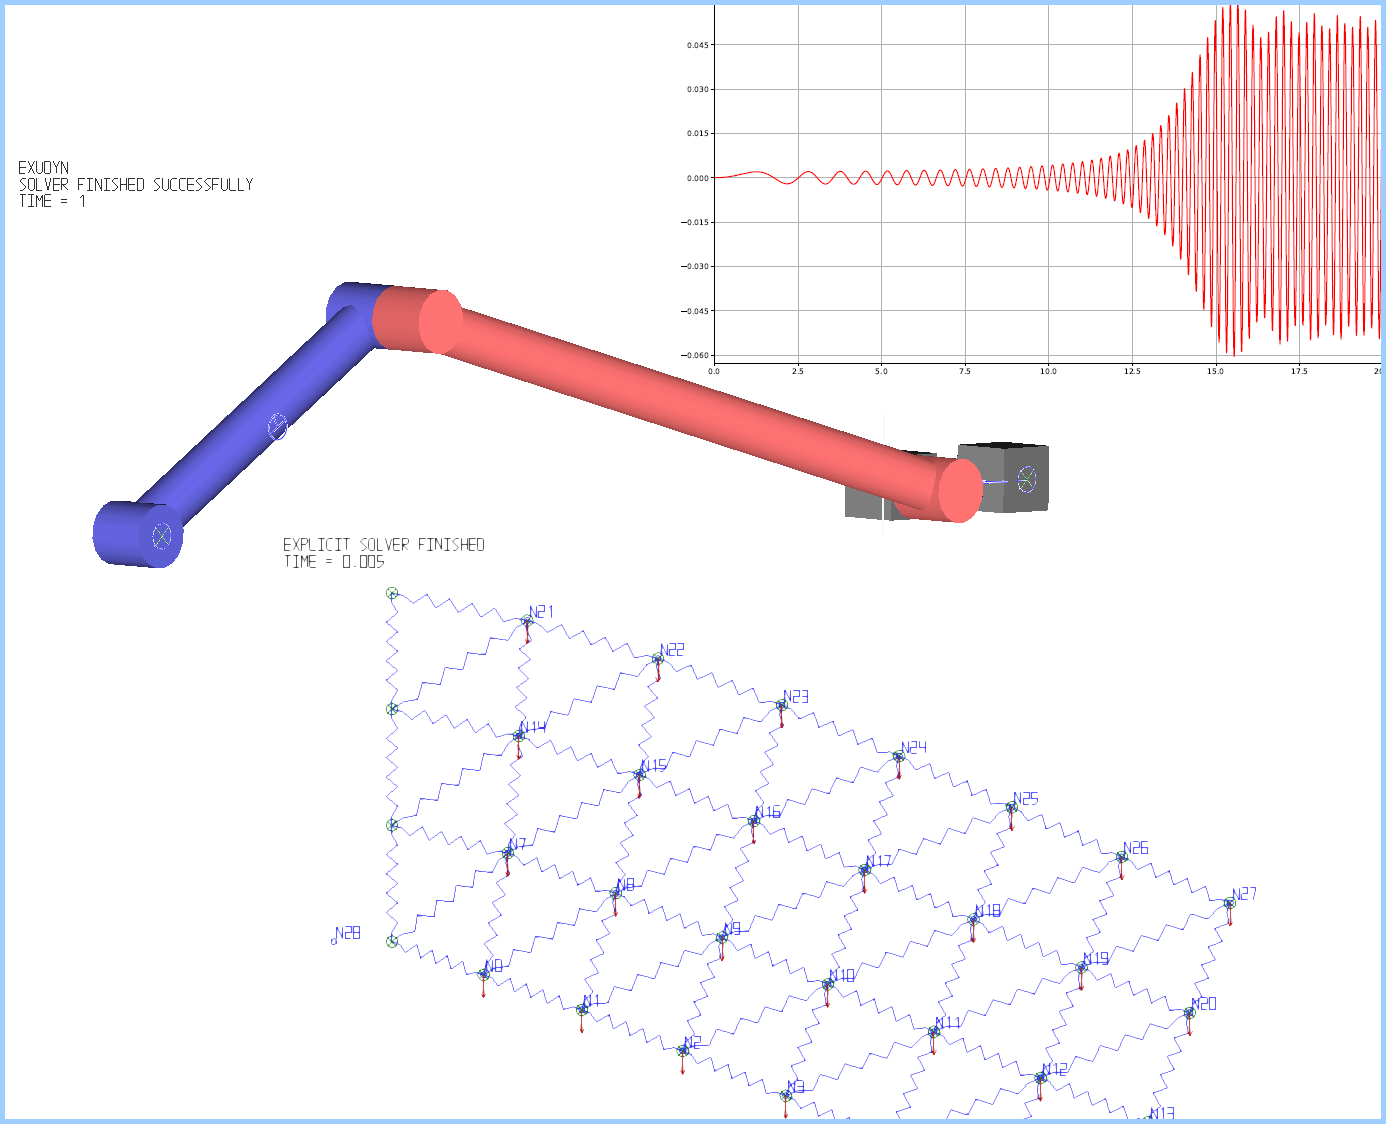
\includegraphics[height=12cm]{intro1.png}\\
\vspace{0.5cm}
{\tiny % version info automatically generated by tracker; generated by Johannes Gerstmayr
% last modified = 2021-05-11
EXUDYN version = 1.0.218
}\\
\vspace{1.5cm}
University of Innsbruck, Department of Mechatronics, \today,\vspace{0.25cm}\\
Johannes Gerstmayr\vspace{2cm}
\end{center}

\newpage

\pagestyle{plain}
\headsep0.7cm 
%\headsep1cm 
%\chapter*{Contents}
%
\tableofcontents


%%++++++++++++++++++++++++++++++++++++++++++++++
\clearpage
\pagenumbering{arabic} 
\setcounter{page}{0}

%+++++++++++++++++++++++++++++++++++++++++++++++++++++++++++++++++++++++++++++++
\mysection{Getting Started}

%+++++++++++++++++++++++++++++++++++++++++++++++++++++++++++++++++++++++++++++++
%\mysection{Getting Started}
The documentation for \codeName\ is split into this introductory section, including a quick start up, code structure and important hints, 
as well as a couple of sections containing references to the available Python interfaces to interact with \codeName\ and finally some information on theory (e.g., 'Solver').

\codeName\ is hosted on GitHub:
\bi
 \item web: \texttt{https://github.com/jgerstmayr/EXUDYN/wiki}
\ei
For any comments, requests, issues, bug reports, send an email to: 
\bi
  \item email: \texttt{reply.exudyn@gmail.com}
\ei
Thanks for your contribution!

\mysubsection{Getting started}
This section will show:
\bn
	\item What is \codeName ?
	\item Who is developing \codeName ?
	\item How to install \codeName\ 
	\item How to link \codeName\ and Python
	\item Goals of \codeName
	\item Run a simple example in Spyder
	\item FAQ -- Frequently asked questions
\en
%
\mysubsubsection{What is \codeName ?}
\codeName -- {\small (fl{\bf EX}ible m{\bf U}ltibody {\bf DYN}amics  -- {\bf EX}tend yo{\bf U}r {\bf DYN}amics)}\vspace{6pt}\\
\noindent \codeName\ is a C++ based Python library for efficient simulation of flexible multibody dynamics systems.
It is designed to easily set up complex multibody models, consisting of rigid and flexible bodies with joints, loads and other components. It shall enable automized model setup and parameter variations, which are often necessary for system design but also for analysis of technical problems. The broad usability of python allows to couple a multibody simulation with environments such as optimization, statistics, data analysis, machine learning and others.

The multibody formulation is mainly based on redundant coordinates. This means that computational objects (rigid bodies, flexible bodies, ...) are added as independent bodies to the system. Hereafter, connectors (e.g., springs or constraints) are used to interconnect the bodies. The connectors are using Markers on the bodies as interfaces, in order to transfer forces and displacements.
For details on the interaction of nodes, objects, markers and loads see Section \ref{sec_items}.
\vspace{6pt}\\
%
\mysubsubsection{Who is developing \codeName ?}
\codeName\ is currently (\the\month-\the\year) developed at the University of Innsbruck.
In the first phase most of the core code is written by Johannes Gerstmayr, implementing ideas that followed out of the project HOTINT. 15 years of development led to a lot of lessions learned and after 20 years, a code must be re-designed.

Some specific codes regarding Pybind11 (by Jakob Wenzel, \texttt{https://github.com/pybind/pybind11}, thanks a lot!!!) interface and parallelization have been written by Stefan Holzinger, who also supported the upload to GitLab.

Important discussions with researchers from the community were important for the design and development of \codeName , where we like to mention Joachim Sch{\"o}berl from TU-Vienna who boosted the design of the code with great concepts. 
%During a Comet-K2 cooperation project, several discussions with the TMECH/LCM group in Linz influenced the code development.

The cooperation and funding within the EU H2020-MSCA-ITN project 'Joint Training on Numerical Modelling of Highly Flexible Structures for Industrial Applications' contributes to the development of the code.

The following people have contributed to the examples:
\bi
	\item Stefan Holzinger, Michael Pieber, Joachim Sch{\"o}berl, Manuel Schieferle, Martin Knapp, Lukas March, Dominik Sponring, David Wibmer, Andreas Zw{\"o}lfer
\ei
-- thanks a lot! --
%
%++++++++++++++++++++++++++++++++++++++++++++++++++++++++++++++++
%++++++++++++++++++++++++++++++++++++++++++++++++++++++++++++++++
%++++++++++++++++++++++++++++++++++++++++++++++++++++++++++++++++
\mysubsubsection{How to install \codeName ?}

In order to run \codeName , you need an appropriate Python installation.
We recommend to use
\bi
  \item Anaconda, 32bit, Python 3.6.5 or Anaconda 64bit, Python 3.6.5)\footnote{Anaconda 32/64bit with Python3.6 can be downloaded via the repository archive \texttt{https://repo.anaconda.com/archive/} choosing \texttt{Anaconda3-5.2.0-Windows-x86.exe} or \texttt{Anaconda3-5.2.0-Windows-x86\_64.exe} for 64bit.}
	\item Spyder 3.2.8 with Python 3.6.5 32 bit (alternatively 64bit), which is included in the Anaconda installation\footnote{It is important that Spyder, python and exudyn are {\bf either} 32bit {\bf or} 64bit. There will be a strange .DLL error, if you mix up 32/64bit. It is possible to install both, Anaconda 32bit and Anacondo 64bit -- then you should follow the recommendations of paths as suggested by Anaconda installer}
%Anaconda3-5.2.0-Windows-x86\_64.exe
\ei
If you plan to extend the C++ code, we recommend to use VS2017\footnote{previously, VS2019 was recommended: However, VS2019 has problems with the library 'Eigen' and therefore leads to erroneous results with the sparse solver. VS2017 can also be configured with Python 3.7 now.} to compile your code, which offers Python 3.7 compatibility.
However, you should know that Python versions and the version of the module must be identical (e.g., Python 3.6 32 bit {\bf both} in the \codeName\ module and in Spyder).

%The simplest way to start is, to copy the files (and possibly further files that are needed)
%\bi
  %\item \texttt{exudynUtilities.py}
  %\item \texttt{itemInterface.py}
  %\item \texttt{exudyn.pyd}
%\ei
%to your working directory and directly import the modules as described in tutorials and examples.
%+++++++++++++++++++++++++++++++++++++
\mysubsubsection{Install with Windows MSI installer}
The simplest way on Windows 10 (and maybe also Windows 7), which works well {\bf if you installed only one python version} and if you installed Anaconda with the option {\bf 'Register Anaconda as my default Python 3.x'} or similar, then you can use the provided \texttt{.msi} installers in the \texttt{main/dist} directory:
\bi
  \item For the 64bits python 3.6 version, double click on (version may differ):\\ \texttt{exudyn-1.0.6.win-amd64-py3.6.msi}
	\item Follow the instructions of the installer
	\item If python / Anaconda is not found by the installer, provide the 'python directory' as the installation directory of Anaconda3, which usually is installed in:\\
	\texttt{C:$\backslash$ProgramData$\backslash$Anaconda3}
\ei

%+++++++++++++++++++++++++++++++++++++
\mysubsubsection{Install from Wheel}
The {\bf standard way to install} the python package \codeName\ is to use the so-called 'wheels' (file ending \texttt{.whl}) provided at the directory wheels in the \codeName\ repository. 
First, open an Anaconda prompt:
\bi
  \item EITHER calling: START->Anaconda->... OR go to anaconda/Scripts folder and call activate.bat
	\item You can check your python version then, by running \texttt{python}\footnote{\texttt{python3} under UBUNTU 18.04}, the output reads like:
	\bi
	  \item[] \texttt{Python 3.6.5 $|$Anaconda, Inc.$|$ (default, Mar 29 2018, 13:32:41) $[$MSC v.1900 64 bit (AMD64)$]$ on win32}
		\item[] ...
	\ei
	\item $\ra$ type \texttt{exit()} to close python
\ei

\noindent {\bf Go to the folder \texttt{Exudyn\_git/main}} (where \texttt{setup.py} lies) and choose the wheel in subdirectory \texttt{main/dist} according to your system (windows/UBUNTU), python version (3.6 or 3.7) and 32 or 64 bits.

For Windows this may read (version number 1.0.6 may be different):
\bi
  \item \texttt{Python 3.6, 32bit}: pip install dist$\backslash$exudyn-1.0.6-cp36-cp36m-win32.whl
  \item \texttt{Python 3.6, 64bit}: pip install dist$\backslash$exudyn-1.0.6-cp36-cp36m-win\_amd64.whl
  \item \texttt{Python 3.7, 64bit}: pip install dist$\backslash$exudyn-1.0.6-cp37-cp37m-win\_amd64.whl
\ei
For UBUNTU18.04 this may read (version number 1.0.6 may be different):
\bi
  \item \texttt{Python 3.6, 64bit}: pip3 install dist$\backslash$exudyn-1.0.6-cp36-cp36m-linux\_x86\_64.whl
\ei

%+++++++++++++++++++++++++++++++++++++
\mysubsubsection{Work without installation and editing \texttt{sys.path}}
The {\bf uncommon and old way} ($\ra$ not recommended for \codeName\ versions $\ge$ 1.0.0) is to use Python's \texttt{sys} module to link to your \texttt{exudyn} (previously \texttt{WorkingRelease}) directory, for example:\vspace{6pt}\\
\pythonstyle
\begin{lstlisting}[language=Python, firstnumber=1]
  import sys
  sys.path.append('C:/DATA/cpp/EXUDYN_git/bin/EXUDYN32bitsPython36')
\end{lstlisting}
%  sys.path.append('C:/DATA/cpp/EXUDYN_git/main/bin/WorkingRelease')
%
The folder \texttt{EXUDYN32bitsPython36} needs to be adapted to the location of the according \codeName\ package.
%In case of 64bit, it must be changed to \texttt{.... /bin/WorkingRelease64}.

%In the future, there will also be a possibility to install the module using pip commands -- we are happy, if somebody could do this!

%++++++++++++++++++++++++++++++++++++++++++++++++++++++++++++++++++++++++++++++
%++++++++++++++++++++++++++++++++++++++++++++++++++++++++++++++++++++++++++++++
\mysubsubsection{Build and install \codeName\ under Windows 10?}

Note that there are a couple of pre-requisites, depending on your system and installed libraries. For Windows 10, the following steps proved to work:
\bi
  \item install your Anaconda distribution including Spyder
  \item close all Python programs (e.g. Spyder, Jupyter, ...)
	\item run an Anaconda prompt (may need to be run as administrator)
	\item if you cannot run Anaconda prompt directly, do:
	\bi
	  \item open windows shell (cmd.exe) as administrator (START $\ra$ search for cmd.exe $\ra$ right click on app $\ra$ 'run as administrator' if necessary)
		\item go to your Scripts folder inside the Anaconda folder (e.g. \texttt{C:$\backslash$ProgramData$\backslash$Anaconda$\backslash$Scripts})
	  \item run 'activate.bat'
	\ei
	\item go to 'main' of your cloned github folder of exudyn
	\item run: \texttt{python setup.py install}
	\item read the output; if there are errors, try to solve them by installing appropriate modules
\ei
You can also create your own wheels, doing the above steps to activate the according python version and then calling (requires installation of Microsoft Visual Studio; recommended: VS2017):
\bi
  \item[] \texttt{python setup.py bdist\_wheel}
\ei
This will add a wheel in the \texttt{dist} folder.

%++++++++++++++++++++++++++++++++++++++++++++++++++++++++++++++++++++++++++++++
%++++++++++++++++++++++++++++++++++++++++++++++++++++++++++++++++++++++++++++++
\mysubsubsection{Build and install \codeName\ under UBUNTU?}

Having a new UBUNTU 18.04 standard installation (e.g. using a VM virtual box environment), the following steps need to be done (python {\bf 3.6} is already installed on UBUNTU18.04, otherwise use \texttt{sudo apt install python3})\footnote{see also the youtube video: \texttt{https://www.youtube.com/playlist?list=PLZduTa9mdcmOh5KVUqatD9GzVg\_jtl6fx}}:

\noindent First update ...
\begin{lstlisting}[firstnumber=1]
sudo apt-get update
\end{lstlisting}

\noindent Install necessary python libraries and pip3; \texttt{matplotlib} and\texttt{scipy} are not required for installation but used in \codeName\ examples:
\begin{lstlisting}[firstnumber=1]
sudo dpkg --configure -a
sudo apt install python3-pip
pip3 install numpy
pip3 install matplotlib
pip3 install scipy
\end{lstlisting}

\noindent Install pybind11 (needed for running the setup.py file derived from the pybind11 example):
\begin{lstlisting}[firstnumber=1]
pip3 install pybind11
\end{lstlisting}

\noindent If graphics is used (\texttt{\#define USE\_GLFW\_GRAPHICS} in \texttt{BasicDefinitions.h}), you must install the according GLFW and OpenGL libs:
\begin{lstlisting}[firstnumber=1]
sudo apt-get install freeglut3 freeglut3-dev
sudo apt-get install mesa-common-dev
sudo apt-get install libglfw3 libglfw3-dev
sudo apt-get install libx11-dev xorg-dev libglew1.5 libglew1.5-dev libglu1-mesa libglu1-mesa-dev libgl1-mesa-glx libgl1-mesa-dev
\end{lstlisting}

\noindent With all of these libs, you can run the setup.py installer (go to \texttt{Exudyn\_git/main} folder), which takes some minutes for compilation (the --user option is used to install in local user folder):
\begin{lstlisting}[firstnumber=1]
sudo python3 setup.py install --user
\end{lstlisting}

\noindent Congratulation! {\bf Now, run a test example} (will also open an OpenGL window if successful):
\bi
  \item[] \texttt{python3 pythonDev/Examples/rigid3Dexample.py}
\ei

\noindent You can also create a UBUNTU wheel which can be easily installed on the same machine (x64), same operating system (UBUNTU18.04) and with same python version (e.g., 3.6):
\bi
  \item[] \texttt{sudo pip3 install wheel}
  \item[] \texttt{sudo python3 setup.py bdist\_wheel}
\ei

%++++++++++++++++++++++++++++++++++++++++++++++++++++++++++++++++++++++++++++++
\mysubsubsection{Uninstall \codeName }

To uninstall exudyn under Windows, run (may require admin rights):
\bi
  \item[] \texttt{pip uninstall exudyn}
\ei
\noindent To uninstall under UBUNTU, run:
\bi
  \item[] \texttt{sudo pip3 uninstall exudyn}
\ei

If you upgrade to a newer version, uninstall is usually not necessary!
%
%++++++++++++++++++++++++++++++++++++++++++++++++++++++++++++++++
\mysubsubsection{How to install \codeName\ and using the C++ code (advanced)?}
\codeName\ is still under intensive development of core modules.
There are several ways to using the code, but you {\bf cannot} install \codeName\ as compared to other executable programs and apps.
\vspace{6pt}\\
%{\bf Ways to use \codeName }:
In order to make full usage of the C++ code and extending it, you can use:
\bi
	\item Windows / Microsoft Visual Studio 2017 and above:
	\bi
		\item get the files from git
		\item put them into a local directory (recommended: \texttt{C:/DATA/cpp/EXUDYN\_git})
		\item start \texttt{main\_sln.sln} with Visual Studio
		\item compile the code and run \texttt{main/pythonDev/pytest.py} example code
		\item adapt \texttt{pytest.py} for your applications
		\item extend the C++ source code
		\item link it to your own code
		\item NOTE: on Linux systems, you mostly need to replace '$/$' with '$\backslash$'
	\ei
	\item Linux, etc.: not fully supported yet; however, all external libraries are Linux-compatible and thus should run with minimum adaptation efforts.
\ei
%
%++++++++++++++++++++++++++++++++++++++++++++++++++++++++++++++++
%++++++++++++++++++++++++++++++++++++++++++++++++++++++++++++++++
\mysubsubsection{Goals of \codeName}
After the first development phase (planned in Q4/2021), it will
\bi
  \item be a small multibody library, which can be easily linked to other projects,
	\item allow to efficiently simulate small scale systems (compute 100000s time steps per second for systems with $n_{DOF}<10$),
	%\item allow to efficiently simulate medium scaled systems for problems with $n_{DOF} < 1\,000\,000$ (planned: Q4 2020),
	%\item use multi-threaded parallel computing techniques (planned: Q4 2020),
	\item safe and widely accessible module for Python,
	\item allow to add user defined objects in C++,
	%\item allow to add user defined objects in Python (planned: 2021),
	\item allow to add user defined solvers in Python).
\ei
%
%++++++++++++++++++++++++++++++++++++++++++++++++++++++++++++++++
%++++++++++++++++++++++++++++++++++++++++++++++++++++++++++++++++
\mysubsubsection{Run a simple example in Spyder}
After performing the steps of the previous section, this section shows a simplistic model which helps you to check if \codeName\ runs on your computer.

In order to start, run the python interpreter Spyder.
For the following example, either 
\bi
	\item open Spyder and copy the example provided in Listing \ref{lst:firstexample} into a new file, or
	\item open \texttt{myFirstExample.py} from your \texttt{EXUDYN32bitsPython36}\footnote{or any other directory according to your python version} directory
\ei
Hereafter, press the play button or \texttt{F5} in Spyder.
%\lstinputlisting[language=Python]{../../main/bin/WorkingRelease/myFirstExample.py}
\pythonexternal[language=Python, frame=single, float, label=lst:firstexample, caption=My first example]{../../main/pythonDev/Examples/myFirstExample.py}

If successful, the IPython Console of Spyder will print something like:
\plainlststyle
{\ttfamily \footnotesize
\begin{lstlisting}
runfile('C:/DATA/cpp/EXUDYN_git/main/bin/EXUDYN32bitsPython36/myFirstExample.py', 
  wdir='C:/DATA/cpp/EXUDYN_git/main/bin/EXUDYN32bitsPython36')
+++++++++++++++++++++++++++++++
EXUDYN V1.0.1 solver: implicit second order time integration
STEP100, t = 1 sec, timeToGo = 0 sec, Nit/step = 1
solver finished after 0.0007824 seconds.
\end{lstlisting}
  %runfile('C:/DATA/cpp/EXUDYN_git/main/bin/WorkingRelease/myFirstExample.py', 
	  %wdir='C:/DATA/cpp/EXUDYN_git/main/bin/WorkingRelease')
}

If you check your current directory (where \texttt{myFirstExample.py} lies), you will find a new file \texttt{coordinatesSolution.txt}, which contains the results of your computation (with default values for time integration).
The beginning and end of the file should look like: \vspace{6pt}\\
{\ttfamily \footnotesize
\begin{lstlisting}[breaklines=true]
  #Exudyn generalized alpha solver solution file
  #simulation started=2019-11-14,20:35:12
  #columns contain: time, ODE2 displacements, ODE2 velocities, ODE2 accelerations, AE coordinates, ODE2 velocities
  #number of system coordinates [nODE2, nODE1, nAlgebraic, nData] = [2,0,0,0]
  #number of written coordinates [nODE2, nVel2, nAcc2, nODE1, nVel1, nAlgebraic, nData] = [2,2,2,0,0,0,0]
  #total columns exported  (excl. time) = 6
  #number of time steps (planned) = 100
  #
  0,0,0,0,0,0.0001,0
  0.02,2e-08,0,2e-06,0,0.0001,0
  0.03,4.5e-08,0,3e-06,0,0.0001,0
  0.04,8e-08,0,4e-06,0,0.0001,0
  0.05,1.25e-07,0,5e-06,0,0.0001,0

  ...

  0.96,4.608e-05,0,9.6e-05,0,0.0001,0
  0.97,4.7045e-05,0,9.7e-05,0,0.0001,0
  0.98,4.802e-05,0,9.8e-05,0,0.0001,0
  0.99,4.9005e-05,0,9.9e-05,0,0.0001,0
  1,5e-05,0,0.0001,0,0.0001,0
  #simulation finished=2019-11-14,20:35:12
  #Solver Info: errorOccurred=0,converged=1,solutionDiverged=0,total time steps=100,total Newton iterations=100,total Newton jacobians=100
\end{lstlisting}
}

Within this file, the first column shows the simulation time and the following columns provide solution of coordinates, their derivatives and Lagrange multipliers on system level. As expected, the $x$-coordinate of the point mass has constant acceleration $a=f/m=0.001/10=0.0001$, the velocity grows up to $0.0001$ after 1 second and the point mass moves $0.00005$ along the $x$-axis.
%
%++++++++++++++++++++++++++++++++++++++++++++++++++++++++++++++++
%++++++++++++++++++++++++++++++++++++++++++++++++++++++++++++++++
\mysubsection{FAQ -- Frequently asked questions}

\bn
  %++++++++++++++++++++++++++++++++++++++++++++++++++++++++++++++++++++++++++++++++++++++++
  %++++++++++++++++++++++++++++++++++++++++++++++++++++++++++++++++++++++++++++++++++++++++
  \item Where do I find the '.exe' file?
	\bi
	\item[$\ra$] \codeName\ is only available via the python interface as exudyn.pyd library, which is located in folder: \texttt{main/bin/WorkingRelease}. This means that you need to run python (best: Spyder) and import the \codeName\ module.
	\ei
	%
  %++++++++++++++++++++++++++++++++++++++++++++++++++++++++++++++++++++++++++++++++++++++++
  %++++++++++++++++++++++++++++++++++++++++++++++++++++++++++++++++++++++++++++++++++++++++
	\item Why does type auto completion does not work for mbs (Main system)?
	\bi
	\item[$\ra$] UPDATE 2020-06-01: with Spyder 4, using Python 3.7, type auto completion works much better. However, note that absolute paths need to be used for module import.
	\item[$\ra$] most python environments (e.g., with Spyder 3) only have information up to the first sub-structure, e.g., \texttt{SC=exu.SystemContainer()} provides full access to SC in the type completion, but \texttt{mbs=SC.AddSystem()} is at the second sub-structure of the module and is not accessible.\\
	WORKAROUND: type \texttt{mbs=MainSystem()} {\bf before} the \texttt{mbs=SC.AddSystem()} command and the interpreter will know what type mbs is. This also works for settings, e.g., simulation settings 'Newton'.
	\ei
	%
  %++++++++++++++++++++++++++++++++++++++++++++++++++++++++++++++++++++++++++++++++++++++++
  %++++++++++++++++++++++++++++++++++++++++++++++++++++++++++++++++++++++++++++++++++++++++
  \item How to add graphics?
	\bi
	\item[$\ra$] Graphics (lines, text, 3D triangular / STL mesh) can be added to all BodyGraphicsData items in objects. Graphics objects which are fixed with the background can be attached to a ObjectGround object.
	Moving objects must be attached to the BodyGraphicsData of a moving body. Other moving bodies can be realized, e.g., by adding a ObjectGround and changing its reference with time.
	\ei
  %++++++++++++++++++++++++++++++++++++++++++++++++++++++++++++++++++++++++++++++++++++++++
  %++++++++++++++++++++++++++++++++++++++++++++++++++++++++++++++++++++++++++++++++++++++++
  \item What is the difference between MarkerBodyPosition and MarkerBodyRigid?
	\bi
	\item[$\ra$] Position markers (and nodes) do not have information on the orientation (rotation). For that reason, there is a difference between position based and rigid-body based markers. In case of a rigid body attached to ground with a SpringDamper, you can use both, MarkerBodyPosition or MarkerBodyRigid, markers. For a prismatic joint, you will need a MarkerBodyRigid.
	\ei
  %++++++++++++++++++++++++++++++++++++++++++++++++++++++++++++++++++++++++++++++++++++++++
  %++++++++++++++++++++++++++++++++++++++++++++++++++++++++++++++++++++++++++++++++++++++++
  \item I do not understand the python errors -- how can I find the reason of the error or crash?
	\bi
	\item[$\ra$] First, you should read all error messages and warnings: from the very first to the last message. Very often, there is a definite line number which shows the error. Note, that if you are executing a string (or module) as a python code, the line numbers refer to the local line number inside the script or module.
	\item[$\ra$] If everything fails, try to execute only part of the code to find out where the first error occurs. By omiting parts of the code, you should find the according source of the error.
	\item[$\ra$] If you think, it is a bug: send an email with a representative code snippet, version, etc.\ to \texttt{ reply.exudyn@gmail.com}
	\ei
  %++++++++++++++++++++++++++++++++++++++++++++++++++++++++++++++++++++++++++++++++++++++++
  %++++++++++++++++++++++++++++++++++++++++++++++++++++++++++++++++++++++++++++++++++++++++
  \item I get an error in \texttt{SC.TimeIntegrationSolve(mbs, 'GeneralizedAlpha', simulationSettings)} but no further information -- how can I solve it?
	\bi
	\item[$\ra$] Typical time integration errors may look like:\\
	{\footnotesize
  \texttt{File "C:/DATA/cpp/EXUDYN\_git/main/pythonDev/...<file name>", line XXX, in <module>}\\  
	\texttt{SC.TimeIntegrationSolve(mbs, 'GeneralizedAlpha', simulationSettings)}\\
  \texttt{SystemError: <built-in method TimeIntegrationSolve of PyCapsule object at 0x0CC63590> returned a result with an error set}}
	\item[$\ra$] The prechecks, which are performed to enable a crash-free simulation are insufficient for your model.
	\item[$\ra$] Very likely, you are using python user functions inside EXUDYN: They lead to an internal python error, which is not catched by EXUDYN. However, you can just check all your user functions, if they will run without EXUDYN. E.g., a load user function UFload(t,load), which tries to access load[4] will fail internally.
	\item[$\ra$] Use the print(...) command in python at many places to find a possible error in user functions (e.g., put \texttt{print("Start user function XYZ")} at the beginning of every user function.
	\item[$\ra$] It is also possible, that you are using inconsistent data, which leads to the crash. In that case, you should try to change your model: omit parts and find out which part is causing your error
	\item[$\ra$] see also {\it I do not understand the python errors -- how can I find the cause?}
 	\ei


  %++++++++++++++++++++++++++++++++++++++++++++++++++++++++++++++++++++++++++++++++++++++++
  %++++++++++++++++++++++++++++++++++++++++++++++++++++++++++++++++++++++++++++++++++++++++
  \item Why can't I get the focus of the simulation window on startup (render window hidden)?
	\bi
	\item[$\ra$] Starting \codeName\ out of Spyder might not bring the simulation window to front, because of specific settings in Spyder(version 3.2.8), e.g., Tools$\ra$Preferences$\ra$Editor$\ra$Advanced settings: uncheck 'Maintain focus in the Editor after running cells or selections'; Alternatively, set \texttt{SC.visualizationSettings.window.alwaysOnTop=True} {\bf before} starting the renderer with \texttt{exu.StartRenderer()}
	\ei
	%
  %++++++++++++++++++++++++++++++++++++++++++++++++++++++++++++++++++++++++++++++++++++++++
  %++++++++++++++++++++++++++++++++++++++++++++++++++++++++++++++++++++++++++++++++++++++++
  \item When importing \codeName\ in python (windows) I get the error (or similar):\\
{\ttfamily \footnotesize
\begin{lstlisting}[breaklines=true]
Traceback (most recent call last):
  File "C:\DATA\cpp\EXUDYN_git\main\pythonDev\pytest.py", line 18, in <module>
    import exudyn as exu
  ImportError: DLL load failed: %1 is no valid Win32 application.
\end{lstlisting}}
	$\ra$ probably this is a 32/64bit problem. Your Python installation and \codeName\ need to be {\bf BOTH} either 64bit OR 32bit (Check in your python help; exudyn in WorkingRelease64 is the 64bit version, in WorkingRelease it is the 32bit version) and the Python installation and \codeName\ need to have {\bf BOTH} the same version and 1$\mathrm{st}$ subversion number (e.g., 3.6.5 should be compatible with 3.6.2).
\en




\mysection{Overview on \codeName }

\mysubsection{Module structure} \label{sec:programStructure}
This section will show:
\bi
  \item Overview of modules
  \item Conventions: dimension of nodes, objects and vectors
	\item Coordinates: reference coordinates and displacements
	\item Nodes, Objects, Markers and Loads
\ei
For an introduction to the solvers, see \refSection{sec:solvers}.

\mysubsubsection{Overview of modules}
Currently, the module structure is simple:
\bi
  \item Python parts:
	\bi
	  \item \texttt{itemInterface}: contains the interface, which transfers python classes (e.g., of a NodePoint) to dictionaries that can be understood by the C++ module
	  \item \texttt{exudynUtilities}: constains helper classes in Python, which allows simpler working with EXUDYN
	\ei
  \item C++ parts, see Figs.\ \ref{fig_exudyn_overview} and \ref{fig_system_overview}:
	\bi
	  \item \texttt{exudyn}\footnote{For versions < 1.0.0: there is a second module, called exudynFast, which deactivates all range-, index- or memory allocation checks at the gain of higher speed (probably 30 percent in regular cases and up to 100 percent in the 64 bit version). This module is included by \texttt{import exudynFast as exu} and can be used same as exudyn. To check the version, just type exu.\_\_doc\_\_ and you will see a note on 'exudynFast' in the exudynFast module.}: on this level, there are just very few functions: SystemContainer(), StartRenderer(), StopRenderer()
	  \item \texttt{SystemContainer}: contains the systems (most important), solvers (static, dynamics, ...), visualization settings
	  \item \texttt{mbs}: system created with \texttt{mbs = SC.AddSystem()}, this structure contains everything that defines a solvable multibody system; a large set of nodes, objects, markers, 
		loads can added to the system, see \refSection{sec:item:reference:manual};
		\item \texttt{mbs.systemData}: contains the initial, current, visualization, ... states of the system and holds the items, see \fig{fig_system_overview}
	\ei
\ei
%
%++++++++++++++++++++++++++++++++++++++++++++++++++++++++++++++++++++++++
\begin{figure}
  \centering
	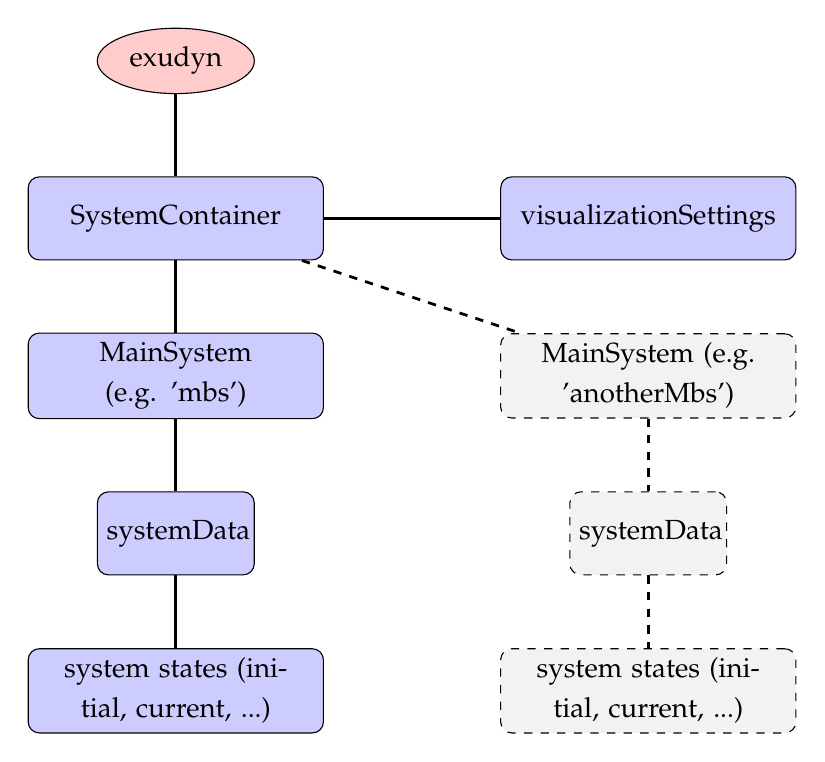
\begin{tikzpicture}[node distance = 2cm, auto]
			% Place nodes
			\node [cloud] (exu) {exudyn};
			\node [wideblock, below of=exu] (systemContainer) {SystemContainer};
			\node [wideblock, below of=systemContainer] (system) {MainSystem (e.g. 'mbs')};
			\node [wideblock, right of=systemContainer,  node distance=6cm] (visualizationSettings) {visualizationSettings};
			\node [block, below of=system] (systemData) {systemData};
			\node [wideblock, below of=systemData] (systemStates) {system states (initial, current, ...)};
			
			\node [wideblock, dashed, fill=gray!10, right of=system,  node distance=6cm] (anotherSystem) {MainSystem (e.g. 'anotherMbs')};
			\node [block, dashed, fill=gray!10, below of=anotherSystem] (anotherSystemData) {systemData};
			\node [wideblock, dashed, fill=gray!10, below of=anotherSystemData] (anotherSystemStates) {system states (initial, current, ...)};

			%\node [cloud, right of=exu] (itemInterface) {itemInterface.py};
			%\node [cloud, right of=itemInterface] (exudynUtilities) {exudynUtilities.py};

			% Draw edges
			\path [line] (exu) -- (systemContainer);
			\path [line] (systemContainer) -- (system);
			\path [line] (systemContainer) -- (visualizationSettings);
			\path [line] (system) -- (systemData);
			\path [line] (systemData) -- (systemStates);

			\path [line, dashed] (systemContainer) -- (anotherSystem);
			\path [line, dashed] (anotherSystem) -- (anotherSystemData);
			\path [line, dashed] (anotherSystemData) -- (anotherSystemStates);
	\end{tikzpicture}
  \caption{Overview of exudyn module.}
	\label{fig_exudyn_overview}
\end{figure}
%++++++++++++++++++++++++++++++++++++++++++++++++++++++++++++++++++++++++

%++++++++++++++++++++++++++++++++++++++++++++++++++++++++++++++++++++++++
\begin{figure}
  \centering
	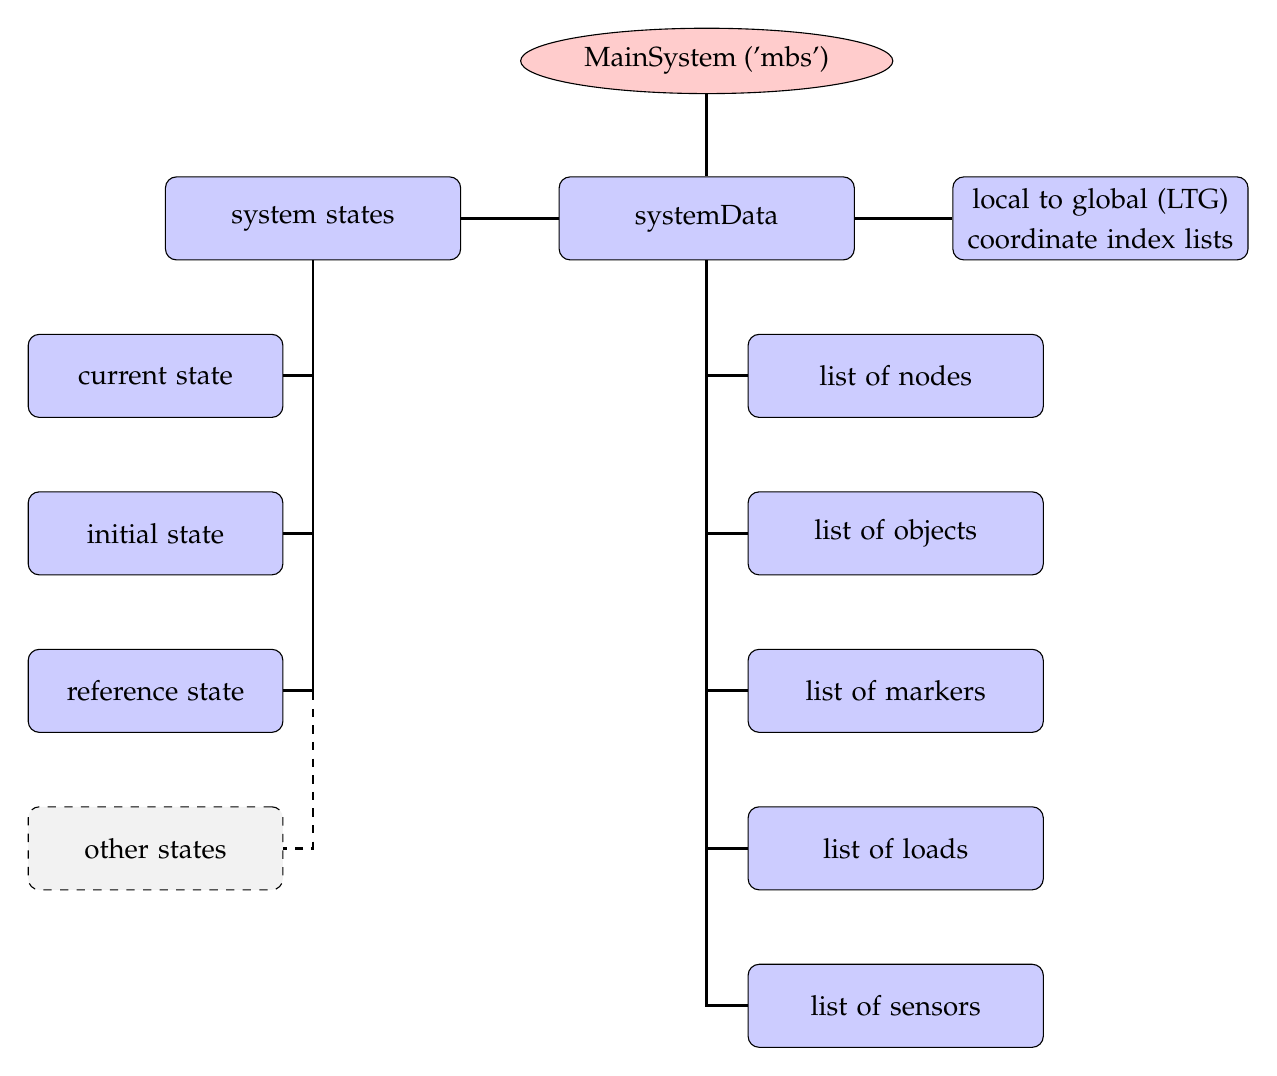
\begin{tikzpicture}[node distance = 2cm, auto]
			% 
			\node [cloud] (system) {MainSystem ('mbs')};
			\node [wideblock, below of=system] (systemData) {systemData};
			\node [wideblock, left of=systemData, node distance=5cm] (systemStates) {system states};
			\node [wideblock, text width=3cm, below of=systemStates, xshift=-2cm] (current) {current state};
			\node [wideblock, text width=3cm, below of=current] (initial) {initial state};
			\node [wideblock, text width=3cm, below of=initial] (reference) {reference state};
			\node [wideblock, text width=3cm, dashed, fill=gray!10, below of=reference] (otherStates) {other states};
			
			\node [wideblock, right of=systemData, node distance=5cm] (ltg) {local to global (LTG) coordinate index lists};
			
			\node [wideblock, below of=systemData, xshift=2.4cm] (nodes) {list of nodes};
			\node [wideblock, below of=nodes] (objects) {list of objects};
			\node [wideblock, below of=objects] (markers) {list of markers};
			\node [wideblock, below of=markers] (loads) {list of loads};
			\node [wideblock, below of=loads] (sensors) {list of sensors};

			% Draw edges
			\path [line] (system) -- (systemData);
			\path [line] (systemData) -- (systemStates);
			\path [line] (systemStates) |- (current);
			\path [line] (systemStates) |- (initial);
			\path [line] (systemStates) |- (reference);
			\path [line, dashed] (systemStates) |- (otherStates);

			\path [line] (systemData) -- (ltg);

			\path [line] (systemData) |- (nodes);
			\path [line] (systemData) |- (objects);
			\path [line] (systemData) |- (markers);
			\path [line] (systemData) |- (loads);
			\path [line] (systemData) |- (sensors);
%
	\end{tikzpicture}
  \caption{Overview of systemData, which connects items and states. Note that access to items is provided via functions in \texttt{system}.}
	\label{fig_system_overview}

\end{figure}
%++++++++++++++++++++++++++++++++++++++++++++++++++++++++++++++++++++++++


\mysubsubsection{Conventions: items, indices, coordinates}
In this documentation, we will use the term {\bf item} to identify nodes, objects, markers and loads:
\be
  \mathrm{item} \in \{\mathrm{node}, \mathrm{object}, \mathrm{marker}, \mathrm{load} \}
\ee
\vspace{12pt}\\
{\bf Indices: arrays and vector starting with 0:} \vspace{6pt}\\
As known from Python, all {\bf indices} of arrays, vectors, etc.\ are starting with 0. This means that the first component of the vector \texttt{v=[1,2,3]} is accessed with \texttt{v[0]} in Python (and also in the C++ part of \codeName ). The range is usually defined as \texttt{range(0,3)}, in which '3' marks the index after the last valid component of an array or vector.
%
\vspace{12pt}\\
{\bf Dimensionality of objects and vectors:}\vspace{6pt}\\ 
As a convention, quantities in \codeName\ are 3D, such as nodes, objects, markers, loads, measured quantities, etc. 
For that reason, we denote planar nodes, objects, etc.\ with the suffix '2D', but 3D objects do not get this suffix.

Output and input to objects, markers, loads, etc.\ is usually given by 3D vectors (or matrices), such as (local) position, force, torque, rotation, etc. However, initial and reference values for nodes depend on their dimensionality.
As an example, consider a \texttt{NodePoint2D}:
\bi
  \item \texttt{referenceCoordinates} is a 2D vector (but could be any dimension in general nodes)
	\item measuring the current position of \texttt{NodePoint2D} gives a 3D vector
	\item when attaching a \texttt{MarkerNodePosition} and a \texttt{LoadForceVector}, the force will be still a 3D vector
\ei
Furthermore, the local position in 2D objects is provided by a 3D vector. Usually, the dimensionality is given in the reference manual. User errors in the dimensionality will be usually detected either by the python interface (i.e., at the time the item is created) or by the system-preprocessor

\mysubsection{Items: Nodes, Objects, Loads, Markers, Sensors, ...} \label{sec:items}
%
In this section, the most important part of \codeName\ are provided. An overview of the interaction of the items is given in \fig{fig_items_interaction}

%++++++++++++++++++++++++++++++++++++++++++++++++++++++++++++++++++++++++
\begin{figure}
  \centering
	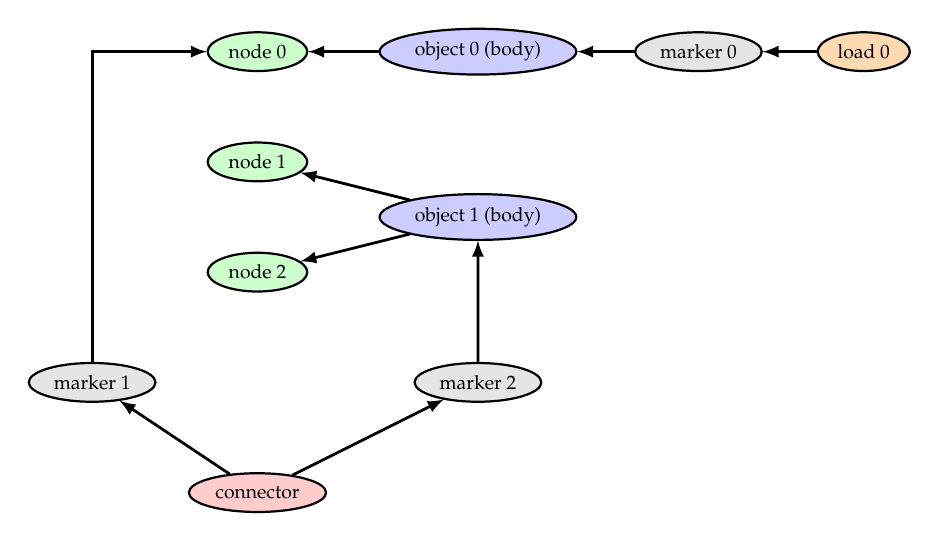
\begin{tikzpicture}[node distance = 2cm, auto, thick,scale=0.7, every node/.style={scale=0.7}]
			% Place nodes
			\node [nodeBlock] (node0) {node 0};
			\node [nodeBlock, below of=node0, node distance=2cm] (node1) {node 1};
			\node [nodeBlock, below of=node1, node distance=2cm] (node2) {node 2};

			\node [objectBlock, right of=node0] (object0) {object 0 (body)};
			\node [objectBlock, right of=node1, yshift = -1cm] (object1) {object 1 (body)};
			
			\node [markerBlock, right of=object0] (marker0) {marker 0};
			\node [loadBlock, right of=marker0, node distance=3cm] (load0) {load 0};
			
			\node [markerBlock, left of=node2, yshift = -2cm, xshift = 1cm] (marker1) {marker 1};
			\node [markerBlock, right of=node2, yshift = -2cm] (marker2) {marker 2};

			\node [connectorBlock, below of=node2] (connector) {connector};


			\path [arrow] (object0) -- (node0);
			\path [arrow] (marker0) -- (object0);
			\path [arrow] (load0) -- (marker0);
			\path [arrow] (object1) -- (node1);
			\path [arrow] (object1) -- (node2);
			\path [arrow] (marker1) |- (node0);
			\path [arrow] (marker2) -- (object1);
			\path [arrow] (connector) -- (marker1);
			\path [arrow] (connector) -- (marker2);
			%\path [line] (systemData) |- (objects);
			%\path [line] (systemData) |- (markers);
			%\path [line] (systemData) |- (loads);

	\end{tikzpicture}
  \caption{Typical interaction of items in a multibody system. Note that both, bodies and connectors/constraints are (computational) objects. The arrows indicate, that, e.g., object 1 has node 1 and node 2 (indices) and that marker 0 is attached to object 0, while load 0 uses marker 0 to apply the load. Sensors could additionally be attached to certain items.}
	\label{fig_items_interaction}

\end{figure}
%++++++++++++++++++++++++++++++++++++++++++++++++++++++++++++++++++++++++

\mysubsubsection{Nodes}
Nodes provide the coordinates (and the degrees of freedom) to the system. They have no mass, stiffness or whatsoever assigned.
Without nodes, the system has no unknown coordinates.
Adding a node provides (for the system unknown) coordinates. In addition we also need equations for every nodal coordinate -- otherwise the system cannot be computed (NOTE: this is currently not checked by the preprocessor).

\mysubsubsection{Objects}
Objects are 'computational objects' and they provide equations to your system. Objects additionally often provide derivatives and have measurable quantities (e.g. displacement) and they provide access, which can be used to apply, e.g., forces.

Objects can be a:
\bi
  \item general object (e.g.\ a controller, user defined object, ...; no example yet)
	\item body: has a mass or mass distribution; markers can be placed on bodies; loads can be applied; constraints can be attached via markers; bodies can be:
	\bi
	  \item[--] ground object: has no nodes
	  \item[--] simple body: has one node (e.g. mass point, rigid body)
	  \item[--] finite element and more complicated body (e.g. FFRF-object): has more than one node
	\ei
	\item connector: uses markers to connect nodes and/or bodies; adds additional terms to system equations either based on stiffness/damping or with constraints (and Lagrange multipliers). Possible connectors:
	\bi
		\item[--] algebraic constraint (e.g. constrain two coordinates: $q_1 = q_2$)
		\item[--] classical joint
		\item[--] spring-damper or penalty constraint
	\ei
\ei

\mysubsubsection{Markers}
Markers are interfaces between objects/nodes and constraints/loads.
A constraint (which is also an object) or load cannot act directly on a node or object without a marker.
As a benefit, the constraint or load does not need to know whether it is applied, e.g., to a node or to a local position of a body.

Typical situations are:
\bi
  \item Node -- Marker -- Load
	\item Node -- Marker -- Constraint (object)
	\item Body(object) -- Marker -- Load
	\item Body1 -- Marker1 -- Joint(object) -- Marker2 -- Body2
\ei

\mysubsubsection{Loads}
Loads are used to apply forces and torques to the system. The load values are static values. However, you can use Python functionality to modify loads either by linearly increasing them during static computation or by using the 'mbs.SetPreStepUserFunction(...)' structure in order to modify loads in every integration step depending on time or on measured quantities (thus, creating a controller).

\mysubsubsection{Sensors}
Sensors are only used to measure output variables (values) in order to simpler generate the requested output quantities.
They have a very weak influence on the system, because they are only evaluated after certain solver steps as requested by the user.

\mysubsubsection{Reference coordinates and displacements}
Nodes usually have separated reference and initial quantities. Here, 
\texttt{referenceCoordinates} are the coordinates for which the system is defined upon creation. Reference coordinates are needed, e.g., for definition of joints and for the reference configuration of finite elements. In many cases it marks the undeformed configuration (e.g., with finite elements), but not, e.g., for \texttt{ObjectConnectorSpringDamper}, which has its own reference length. 

Initial displacement (or rotation) values are provided separately, in order to start a system from a configuration different from the reference configuration.
As an example, the initial configuration of a \texttt{NodePoint} is given by \texttt{referenceCoordinates + initialCoordinates}, while the initial state of a dynamic system additionally needs \texttt{initialVelocities}.


\mysubsection{Exudyn Basics} \label{sec:exudynBasics}
This section will show:
\bi
	\item Interaction with the \codeName\ module
	\item Simulation settings
	\item Visualization settings
	\item Generating output and results
	\item Graphics pipeline
	\item Generating animations
\ei


\mysubsubsection{Interaction with the \codeName\ module}
It is important that the \codeName\ module is basically a state machine, where you create items on the C++ side using the Python interface. This helps you to easily set up models using many other Python modules (numpy, sympy, matplotlib, ...) while the computation will be performed in the end on the C++ side in a very efficient manner. 
\vspace{12pt}\\
{\bf Where do objects live?}\vspace{6pt}\\
%(where do objects live? state machine; graphics interaction)
Whenever a system container is created with \texttt{SC = exu.SystemContainer()}, the structure \texttt{SC} lives in C++ and will be modified via the python interface.
Usually, the system container will hold at least one system, usually called \texttt{mbs}.
Commands such as \texttt{mbs.AddNode(...)} add objects to the system \texttt{mbs}. 
The system will be prepared for simulation by \texttt{mbs.Assemble()} and can be solved (e.g., using \texttt{exu.SolveDynamic(...)}) and evaluated hereafter using the results files.
Using \texttt{mbs.Reset()} will clear the system and allows to set up a new system. Items can be modified (\texttt{ModifyObject(...)}) after first initialization, even during simulation.
%

\mysubsubsection{Simulation settings}
The simulation settings consists of a couple of substructures, e.g., for \texttt{solutionSettings}, \texttt{staticSolver}, \texttt{timeIntegration} as well as a couple of general options -- for details see Sections \ref{sec:SolutionSettings} -- \ref{sec:SimulationSettings}.

Simulation settings are needed for every solver. They contain solver-specific parameters (e.g., the way how load steps are applied), information on how solution files are written, and very specific control parameters, e.g., for the Newton solver. 

The simulation settings structure is created with 
\pythonstyle
\begin{lstlisting}[language=Python, firstnumber=1]
  simulationSettings = exu.SimulationSettings()
\end{lstlisting}
%
Hereafter, values of the structure can be modified, e.g.,
\begin{lstlisting}[language=Python, firstnumber=1]
	#10 seconds of simulation time:
  simulationSettings.timeIntegration.endTime = 10                    
	#1000 steps for time integration:
  simulationSettings.timeIntegration.numberOfSteps = 1000            
	#assigns a new tolerance for Newton's method:
  simulationSettings.timeIntegration.newton.relativeTolerance = 1e-9 
	#write some output while the solver is active (SLOWER):
  simulationSettings.timeIntegration.verboseMode = 2                 
	#write solution every 0.1 seconds:
  simulationSettings.solutionSettings.solutionWritePeriod = 0.1      
  #use sparse matrix storage and solver (package Eigen):
  simulationSettings.linearSolverType = exu.LinearSolverType.EigenSparse 
\end{lstlisting}

\mysubsubsection{Visualization settings}
%
Visualization settings are used for user interaction with the model. E.g., the nodes, markers, loads, etc., can be visualized for every model. There are default values, e.g., for the size of nodes, which may be inappropriate for your model. Therefore, you can adjust those parameters. In some cases, huge models require simpler graphics representation, in order not to slow down performance -- e.g., the number of faces to represent a cylinder should be small if there are 10000s of cylinders drawn. Even computation performance can be slowed down, if visualization takes lots of CPU power. However, visualization is performed in a separate thread, which usually does not influence the computation exhaustively.
Details on visualization settings and its substructures are provided in Sections \ref{sec:VSettingsGeneral} -- \ref{sec:VisualizationSettings}.

The visualization settings structure can be accessed in the system container \texttt{SC} (access per reference, no copying!), accessing every value or structure directly, e.g.,
\pythonstyle
\begin{lstlisting}[language=Python, firstnumber=1]
  SC.visualizationSettings.nodes.defaultSize = 0.001      #draw nodes very small

  #change openGL parameters; current values can be obtained from SC.GetRenderState()
  #change zoom factor:
  SC.visualizationSettings.openGL.initialZoom = 0.2       
  #set the center point of the scene (can be attached to moving object):
  SC.visualizationSettings.openGL.initialCenterPoint = [0.192, -0.0039,-0.075]

  #turn of auto-fit:
  SC.visualizationSettings.general.autoFitScene = False

  #change smoothness of a cylinder:
  SC.visualizationSettings.general.cylinderTiling = 100
	
	#make round objects flat:
	SC.visualizationSettings.openGL.shadeModelSmooth = False

	#turn on coloured plot, using y-component of displacements:
	SC.visualizationSettings.contour.outputVariable = exu.OutputVariableType.Displacement
	SC.visualizationSettings.contour.outputVariableComponent = 1 #0=x, 1=y, 2=z
\end{lstlisting}

\mysubsubsubsection{Storing the model view}
\label{sec:storing:modelview}
There is a simple way to store the current view (zoom, centerpoint, orientation, etc.) by using \texttt{SC.GetRenderState()} and \texttt{SC.SetRenderState()}.
%
A simple way is to reload the stored render state (model view) after simulating your model once at the end of the simulation\footnote{
note that \texttt{visualizationSettings.general.autoFitScene} should be set False if you want to use the stored zoom factor}:
\pythonstyle
\begin{lstlisting}[language=Python, firstnumber=1]
import exudyn as exu
SC=exu.SystemContainer()
SC.visualizationSettings.general.autoFitScene = False #prevent from autozoom
exu.StartRenderer()
if 'renderState' in exu.sys:
    SC.SetRenderState(exu.sys['renderState']) 
#+++++++++++++++
#do simulation here and adjust model view settings with mouse
#+++++++++++++++

#store model view for next run:
StopRenderer() #stores render state in exu.sys['renderState']
\end{lstlisting}
\par\noindent\rule{\textwidth}{0.4pt}
%
Alternatively, you can obtain the current model view from the console after a simulation, e.g.,
\pythonstyle
\begin{lstlisting}
In[1] : SC.GetRenderState()
Out[1]: 
{'centerPoint': [1.0, 0.0, 0.0],
 'maxSceneSize': 2.0,
 'zoom': 1.0,
 'currentWindowSize': [1024, 768],
 'modelRotation': [[ 0.34202015,  0.        , 0.9396926 ],
                   [-0.60402274,  0.76604444, 0.21984631],
                   [-0.7198463 , -0.6427876 , 0.26200265]])}
\end{lstlisting}
%
which contains the last state of the renderer.
Now copy the output and set this with \texttt{SC.SetRenderState} in your Python code to have a fixed model view in every simulation (\texttt{SC.SetRenderState} AFTER \texttt{exu.StartRenderer()}):
\pythonstyle
\begin{lstlisting}[language=Python, firstnumber=1]
SC.visualizationSettings.general.autoFitScene = False #prevent from autozoom
exu.StartRenderer()
renderState={'centerPoint': [1.0, 0.0, 0.0],
             'maxSceneSize': 2.0,
             'zoom': 1.0,
             'currentWindowSize': [1024, 768],
             'modelRotation':     [[ 0.34202015,  0.        ,  0.9396926 ],
                                  [-0.60402274,  0.76604444,  0.21984631],
                                  [-0.7198463 , -0.6427876 ,  0.26200265]])
SC.SetRenderState(renderState)
#.... further code for simulation here
\end{lstlisting}
\par\noindent\rule{\textwidth}{0.4pt}
%
%

\mysubsubsection{Generating output and results}
%
The solvers provide a number of options in \texttt{solutionSettings} to generate a solution file. As a default, exporting solution to the solution file is activated with a writing period of 0.01 seconds.

Typical output settings are:
\pythonstyle
\begin{lstlisting}[language=Python, firstnumber=1]
  #create a new simulationSettings structure:
  simulationSettings = exu.SimulationSettings()
	
  #activate writing to solution file:
  simulationSettings.solutionSettings.writeSolutionToFile = True
  #write results every 1ms:
  simulationSettings.solutionSettings.solutionWritePeriod = 0.001
  
  #assign new filename to solution file
  simulationSettings.solutionSettings.coordinatesSolutionFileName= "myOutput.txt"

  #do not export certain coordinates:
  simulationSettings.solutionSettings.exportDataCoordinates = False
\end{lstlisting}


\mysubsubsection{Graphics pipeline}
%deprecated, since there are user functions!: The user cannot interact with the visualization part for now.
There are basically two loops during simulation, which feed the graphics pipeline.
The solver runs a loop:
\bi
  \item compute new step
	\item finish computation step; results are in current state
	\item copy current state to visualization state (thread safe)
	\item signal graphics pipeline that new visualization data is available
\ei
The openGL graphics thread (=separate thread) runs the following loop:
\bi
  \item render openGL scene with a given graphicsData structure (containing lines, faces, text, ...)
  \item go idle for some milliseconds
	\item check if openGL rendering needs an update (e.g. due to user interaction)
	\item[] $\ra$ if update is needed, the visualization of all items is updated -- stored in a graphicsData structure)
	\item check if new visualization data is available and the time since last update is larger than a presribed value, the graphicsData structure is updated with the new visualization state
\ei

\mysubsubsection{Graphics user Python functions}
There are some user functions in order to customize drawing:
\bi
	\item You can assign graphicsData to the visualization to most bodies, such as rigid bodies in order to change the shape. Graphics can also be imported from STL files (\texttt{GraphicsDataFromSTLfileTxt}).
	\item Some objects, e.g., \texttt{ObjectGenericODE2} or \texttt{ObjectRigidBody}, provide customized a function \texttt{graphicsDataUserFunction}. This user function just returns a list of GraphicsData, see \refSection{sec:graphicsData}. With this function you can change the shape of the body in every step of the computation.
	\item Specifically, the \texttt{graphicsDataUserFunction} in \texttt{ObjectGround} can be used to draw any moving background in the scene.
\ei
Note that all kinds of graphicsUserPythonFunctions need to be called from the main (=computation) process as Python functions may not be called from separate threads (GIL). Therefore, the computation thread is interrupted to execute the \texttt{graphicsDataUserFunction} between two time steps, such that the graphics Python user function can be executed. There is a timeout variable for this interruption of the computation with a warning if scenes get too complicated.

\mysubsubsection{Color and RGBA}
Many functions and objects include color information. In order to allow transparency, all colors contain a list of 4 RGBA values, all values being in the range [0..1]:
\bi
  \item red (R) channel 
	\item green (G) channel  
	\item blue (B) channel 
	\item alpha (A) value, representing transparency (A=0: fully transparent, A=1: solid)
\ei
E.g., red color with no transparency is obtained by the color=[1,0,0,1]. Color predefinitions are found in \texttt{exudynGraphicsDataUtilities.py}, e.g., \texttt{color4red} or \texttt{color4steelblue} as well a list of 10 colors \texttt{color4list}, which is convenient to be used in a loop creating objects.

\mysubsubsection{Generating animations}
\label{secGeneratingAnimations}
%
In many dynamics simulations, it is very helpful to create animations in order to better understand the motion of bodies. Specifically, the animation can be used to visualize the model much slower or faster than the model is computed.

Animations are created based on a series of images (frames, snapshots) taken during simulation. It is important, that the current view is used to record these images -- this means that the view should not be changed during the recording of images.
To turn on recording of images during solving, set the following flag to a positive value
\bi
  \item \texttt{simulationSettings.solutionSettings.recordImagesInterval = 0.01}
\ei
which means, that after every 0.01 seconds of simulation time, an image of the current view is taken and stored in the directory and filename (without filename ending) specified by 
\bi
  \item \texttt{SC.visualizationSettings.exportImages.saveImageFileName = "myFolder/frame"}
\ei
By default, a consecutive numbering is generated for the image, e.g., 'frame0000.tga, frame0001.tga,...'. Note that '.tga' files contain raw image data and therefore can become very large.

To create animation files, an external tool FFMPEG is used to efficiently convert a series of images into an animation.
In windows, simple DOS batch files can do the job to convert frames given in the local directory to animations, e.g.:
\plainlststyle
\lstinputlisting[breaklines=true, basicstyle=\ttm]{../userTools/makeAnimations/convertToVideo.bat}
After the video has been created, you should delete the single images:
\plainlststyle
\lstinputlisting[breaklines=true, basicstyle=\ttm]{../userTools/makeAnimations/deleteTGAimages.bat}


%+++++++++++++++++++++++++++++++++++++++++++++++++++++++++++++++++++++++++++++++
%+++++++++++++++++++++++++++++++++++++++++++++++++++++++++++++++++++++++++++++++

\mysubsection{C++ Code}
This section covers some information on the C++ code. For more information see the Open source code and use doxygen.

Exudyn was developed for the efficient simulation of flexible multi-body systems. Exudyn was designed for rapid implementation and testing of new formulations and algorithms in multibody systems, whereby these algorithms can be easily implemented in efficient C++ code. The code is applied to industry-related research projects and applications.

\mysubsubsection{Focus of the C++ code}
{\bf Four principles}: 
\bn
  \item developer-friendly
	\item error minimization
	\item efficiency
	\item user-friendliness
\en
The focus is therefore on:
\bi
    \item A developer-friendly basic structure regarding the C++ class library and the possibility to add new components.
    \item The basic libraries are slim, but extensively tested; only the necessary components are available
    \item Complete unit tests are added to new program parts during development; for more complex processes, tests are available in Python
    \item In order to implement the sometimes difficult formulations and algorithms without errors, error avoidance is always prioritized.
    \item To generate efficient code, classes for parallelization (vectorization and multithreading) are provided. We live the principle that parallelization takes place on multi-core processors with a central main memory, and thus an increase in efficiency through parallelization is only possible with small systems, as long as the program runs largely in the cache of the processor cores. Vectorization is tailored to SIMD commands as they have Intel processors, but could also be extended to GPGPUs in the future.
    \item The user interface (Python) provides a 1:1 image of the system and the processes running in it, which can be controlled with the extensive possibilities of Python.
\ei

\mysubsubsection{C++ Code structure}
The functionality of the code is based on systems (MainSystem/CSystem) representing the multibody system or similar physical systems to be simulated. Parts of the core structure of Exudyn are:
\bi
	\item CSystem / MainSystem: a multibody system which consists of nodes, objects, markers, loads, etc.
	\item SystemContainer: holds a set of systems; connects to visualization (container)
	\item node: used to hold coordinates (unknowns)
	\item (computational) object: leads to equations, using nodes
	\item marker: defines a consistent interface to objects (bodies) and nodes; write access ('AccessFunction') -- provides jacobian and read access ('OutputVariable')
	\item load: acts on an object or node via a marker
	\item computational objects: efficient objects for computation = bodies, connectors, connectors, loads, nodes, ...
	\item visualization objects: interface between computational objects and 3D graphics
	\item main (manager) objects: do all tasks (e.g. interface to visualization objects, GUI, python, ...) which are not needed during computation
	\item static solver, kinematic solver, time integration
	\item python interface via pybind11; items are accessed with a dictionary interface; system structures and settings read/written by direct access to the structure (e.g. SimulationSettings, VisualizationSettings)
	\item interfaces to linear solvers; future: optimizer, eigenvalue solver, ... (mostly external or in python)
\ei


\mysubsubsection{C++ Code: Modules}
The following internal modules are used, which are represented by directories in \texttt{main/src}:
\bi
	\item Autogenerated: item (nodes, objects, markers and loads) classes split into main (management, python connection), visualization and computation
	\item Graphics: a general data structure for 2D and 3D graphical objects and a tiny openGL visualization; linkage to GLFW
    \item Linalg: Linear algebra with vectors and matrices; separate classes for small vectors (SlimVector), large vectors (Vector and ResizableVector), vectors without copying data (LinkedDataVector), and vectors with constant size (ConstVector)
	\item Main: mainly contains SystemContainer, System and ObjectFactory
	\item Objects: contains the implementation part of the autogenerated items
	\item Pymodules: manually created libraries for linkage to python via pybind; remaining linking to python is located in autogenerated folder
	\item pythonGenerator: contains python files for automatic generation of C++ interfaces and python interfaces of items;
	\item Solver: contains all solvers for solving a CSystem
	\item System: contains core item files (e.g., MainNode, CNode, MainObject, CObject, ...)
	\item Tests: files for testing of internal linalg (vector/matrix), data structure libraries (array, etc.) and functions
    \item Utilities: array structures for administrative/managing tasks (indices of objects ... bodies, forces, connectors, ...); basic classes with templates and definitions
\ei

The following main external libraries are linked to Exudyn:
\bi
	\item LEST: for testing of internal functions (e.g. linalg)
	\item GLFW: 3D graphics with openGL; cross-platform capabilities
	\item Eigen: linear algebra for large matrices, linear solvers, sparse matrices and link to special solvers
	\item pybind11: linking of C++ to python
\ei

\mysubsubsection{Code style and conventions}
%
This section provides general coding rules and conventions, partly applicable to the C++ and python parts of the code. Many rules follow common conventions (e.g., google code style, but not always -- see notation):
\bi
    \item write simple code (no complicated structures or uncommon coding)
    \item write readable code (e.g., variables and functions with names that represent the content or functionality; AVOID abbreviations)
    \item put a header in every file, according to Doxygen format
    \item put a comment to every (global) function, member function, data member, template parameter
    \item ALWAYS USE curly brackets for single statements in 'if', 'for', etc.; example: if (i<n) \{i += 1;\}
    \item use Doxygen-style comments (use '//!' Qt style and '@ date' with '@' instead of '\' for commands)
    \item use Doxygen (with preceeding '@') 'test' for tests, 'todo' for todos and 'bug' for bugs
    \item USE 4-spaces-tab
    \item use C++11 standards when appropriate, but not exhaustively
    \item ONE class ONE file rule (except for some collectors of single implementation functions)
    \item add complete unit test to every function (every file has link to LEST library)
    \item avoid large classes (>30 member functions; > 15 data members)
    \item split up god classes (>60 member functions)
    \item mark changed code with your name and date
    \item REPLACE tabs by spaces: Extras->Options->C/C++->Tabstopps: tab stopp size = 4 (=standard) +  KEEP SPACES=YES
\ei

\mysubsubsection{Notation conventions}
%
The following notation conventions are applied ({\bf no exceptions!}):
\bi
		\item use lowerCamelCase for names of variables (including class member variables), consts, c-define variables, ...; EXCEPTION: for algorithms following formulas, e.g., $f = M*q_{tt} + K*q$, GBar, ...
		\item use UpperCamelCase for functions, classes, structs, ...
		\item Special cases for CamelCase: write 'ODEsystem', BUT: 'ODE1Equations'
		\item '[...]Init' ... in arguments, for initialization of variables; e.g. 'valueInit' for initialization of member variable 'value'
		\item use American English troughout: Visualization, etc.
		\item for (abbreviations) in captial letters, e.g. ODE, use a lower case letter afterwards:
		\item do not use consecutive capitalized words, e.g. DO NOT WRITE 'ODEAE'
		\item for functions use \texttt{ODEComputeCoords()}, for variables avoid 'ODE' at beginning: use nODE or write odeCoords
		\item do not use '\_' within variable or function names; exception: derivatives
		\item use name which exactly describes the function/variable: 'numberOfItems' instead of 'size' or 'l'
		\item examples for variable names: secondOrderSize, massMatrix, mThetaTheta
		\item examples for function/class names: \texttt{SecondOrderSize}, \texttt{EvaluateMassMatrix}, \texttt{Position(const Vector3D\& localPosition)}
		\item use the Get/Set...() convention if data is retrieved from a class (Get) or something is set in a class (Set); Use \texttt{const T\& Get()/T\& Get} if direct access to variables is needed; Use Get/Set for pybind11
		\item example Get/Set: \texttt{Real* GetDataPointer()}, \texttt{Vector::SetAll(Real)}, \texttt{GetTransposed()}, \texttt{SetRotationalParameters(...)}, \texttt{SetColor(...)}, ...
		\item use 'Real' instead of double or float: for compatibility, also for AVX with SP/DP
		\item use 'Index' for array/vector size and index instead of size\_t or int
		\item item: object, node, marker, load: anything handled within the computational/visualization systems
\ei

\mysubsubsection{No-abbreviations-rule}
%
The code uses a {\bf minimum set of abbreviations}; however, the following abbreviation rules are used throughout:
In general: DO NOT ABBREVIATE function, class or variable names: GetDataPointer() instead of GetPtr(); exception: cnt, i, j, k, x or v in cases where it is really clear (5-line member functions).

Exceptions to the NO-ABBREVIATIONS-RULE:
\bi
    \item ODE ... ordinary differential equations;
    \item ODE2 ... marks parts related to second order differential equations (SOS2, EvalF2 in HOTINT)
    \item ODE1 ... marks parts related to first order differential equations (ES, EvalF in HOTINT)
    \item AE ... algebraic equations (IS, EvalG in HOTINT); write 'AEcoordinates' for 'algebraicEquationsCoordinates'
    \item 'C[...]' ... Computational, e.g. for ComputationalNode ==> use 'CNode'
    \item min, max ... minimum and maximum
    \item write time derivatives with underscore: \_t, \_tt; example: Position\_t, Position\_tt, ...
    \item write space-wise derivatives ith underscore: \_x, \_xx, \_y, ...
    \item if a scalar, write coordinate derivative with underscore: \_q, \_v (derivative w.r.t. velocity coordinates)
    \item for components, elements or entries of vectors, arrays, matrices: use 'item' throughout
    \item '[...]Init' ... in arguments, for initialization of variables; e.g. 'valueInit' for initialization of member variable 'value'
\ei


%+++++++++++++++++++++++++++++++++++++++++++++++++++++++++++++++++++++++++++++++
%+++++++++++++++++++++++++++++++++++++++++++++++++++++++++++++++++++++++++++++++

\mysubsection{Changes}
\label{sec:changes}
For continuous tracking of changes, see \refSection{sec:issueTracker}.
%
%The following list covers changes in the python interface and functionality:
%\bi \small
	%%+++++++++++++++++++++++++++++++++++++++++++++++++++++++++++++
	%%\item {\bf Version 0.1.2xx $\ra$ Version 0.1.2yy}
	%%\item[] Changes in the implementation / solver (LEADS TO DIFFERENT RESULTS):
	%%\bi
	  %%\item {\bf xxxx}: 
	%%\ei
	%%\item[] Changes in the python interface:
	%%\bi \ttfamily
	  %%\item $\ra$ 
	%%\ei
	%%+++++++++++++++++++++++++++++++++++++++++++++++++++++++++++++
	%\item {\bf Version 1.0.59$\ra$ Version 1.0.61}
	%\bi
	  %\item {\bf Major changes}: Changed interface of \texttt{processing.GeneticOptimization()}; 
	%\ei
	%%+++++++++++++++++++++++++++++++++++++++++++++++++++++++++++++
	%\item {\bf Version 1.0.56$\ra$ Version 1.0.57}
	%\bi
	  %\item {\bf Major changes}: added new submodule \texttt{exudyn.signal}; 
		%\item {\bf Major changes}: \texttt{FilterSignal} renamed into \texttt{FilterSensorOutput} and moved from \texttt{exudyn.utilities} to \texttt{exudyn.signal}
	%\ei
	%%+++++++++++++++++++++++++++++++++++++++++++++++++++++++++++++
	%\item {\bf Version 1.0.49$\ra$ Version 1.0.51}
	%\bi
	%\item user functions can now be set to zero, e.g.:
	%\item[] \phantom{XXXX} \texttt{mbs.AddObject(CoordinateSpringDamper(markerNumbers=[m0,m1],
	%\item[] \phantom{XXXXXXXX} stiffness=k, damping=0.01*k, 
	%\item[] \phantom{XXXXXXXX} springForceUserFunction=0)}
	%\item Exception: for \texttt{visualizationSettings.window.keyPressUserFunction} use \\ \texttt{SC.visualizationSettings.window.ResetKeyPressUserFunction()} to set it to zero
	%\ei
	%%+++++++++++++++++++++++++++++++++++++++++++++++++++++++++++++
	%\item {\bf Version 1.0.42$\ra$ Version 1.0.49}
	%\bi
	%\item {\bf Major changes}: OpenGL default settings for lights and material have been changed; slightly different appearance might result from that! per default, light1 is active as well.
	%\item {\bf Major changes}: Added key callback functionality \texttt{keyPressUserFunction} to \texttt{VisualizationSettings.window}
	%\item added mouse coordinates (OpenGL and screen pixels) to renderState and added a \texttt{GetCurrentMouseCoordinates()} function to SystemContainer
	%\item added mouse coordinates to renderer window (press 'F3')
	%\item identified problems with OpenGL lights; light1 is now working
	%\item solved problems with coordinateSystem
	%\item added a world basis (coordinate system) at origin of model (0,0,0); \\see \texttt{VisualizationSettings.general.drawWorldBasis}
	%\item added flag \texttt{simulateInRealtime} to \texttt{simulationSettings.timeIntegration}
	%\ei
	%%+++++++++++++++++++++++++++++++++++++++++++++++++++++++++++++
	%\item {\bf Version 1.0.38$\ra$ Version 1.0.42}
	%\bi
	%\item completed \texttt{Acceleration} output variables for all relevant objects and nodes; 
	%\item added FilterSignal(...) (\refSection{sec:signal:FilterSignal}) functionality to utilities, which enables numerical differentiation and filtering, using savgol filter, applied to all output values of data loaded from sensors.
	%\item for example, see \texttt{TestModels/objectFFRFreducedOrderAccelerations.py}.
	%\ei
	%%+++++++++++++++++++++++++++++++++++++++++++++++++++++++++++++
	%\item {\bf Version 1.0.37$\ra$ Version 1.0.38}
	%\bi
	%\item \texttt{SC.StopRenderer()} now stores the last renderState in \texttt{exu.sys['renderState']}, which can be used in subsequent simulations to always have the same view and zoom; 
	%for an example, see \refSection{sec:storing:modelview}.
	%\ei
	%%+++++++++++++++++++++++++++++++++++++++++++++++++++++++++++++
	%\item {\bf Version 1.0.32$\ra$ Version 1.0.37}
	%\bi
	%\item added Python interfaces (exudyn/solver.py) for static/dynamic solvers and eigensolvers: exu.SolveStatic(mbs) and exu.SolveDynamic(mbs) $\ra$ recommended to be used in future
	%\item TimeIntegrationSolve and StaticSolve $\ra$ deprecated; get additional return value for success
	%\ei
	%%+++++++++++++++++++++++++++++++++++++++++++++++++++++++++++++
	%\item {\bf Version 1.0.17 $\ra$ Version 1.0.18}
	%\bi
	%\item {\bf removed} AVX compilation flag for Python 3.6 32bits version due to incompatibility on older Celeron processors
	%\item added acceleration sensor functionality to most objects and nodes
	%\item added Lie group utilities (see \texttt{exudyn.lieGroup})
	%\item added processing utilities for parameter variation and optimization (see \texttt{exudyn.processing})
	%\ei
	%%+++++++++++++++++++++++++++++++++++++++++++++++++++++++++++++
	%\item {\bf Version 1.0.12 $\ra$ Version 1.0.13}
	%\item[] corrected LHS (left-hand-side) and RHS (right-hand-side) terminology (issue: 330), see \refSection{eq_equationLHSRHS}:
	%\bi
	  %\item objects, connectors, etc., use LHS conventions: all terms (mass, stiffness, elastic forces, damping) are computed at LHS of equation
		%\item forces are written at the RHS
		%\item system quantities are always written on RHS: $m \ddot q = f_{RHS}$
	%\ei
	%%+++++++++++++++++++++++++++++++++++++++++++++++++++++++++++++
	%\item {\bf Version 1.0.8 $\ra$ Version 1.0.9}
	%\item[] change from Index in mbs.AddNode(...), mbs.AddObject, ... to special 'item indices' (issue: 333):
	%\bi %\ttfamily
	%\item before: \texttt{mbs.AddNode(...)} $\ra$ Index; {\bf now}: \texttt{mbs.AddNode(...)} $\ra$ NodeIndex
	%\item before: \texttt{mbs.AddObject(...)} $\ra$ Index; {\bf now}: \texttt{mbs.AddObject(...)} $\ra$ ObjectIndex
	%\item before: \texttt{mbs.AddMarker(...)} $\ra$ Index; {\bf now}: \texttt{mbs.AddMarker(...)} $\ra$ MarkerIndex
	%\item before: \texttt{mbs.AddLoad(...)} $\ra$ Index; {\bf now}: \texttt{mbs.AddLoad(...)} $\ra$ LoadIndex
	%\item before: \texttt{mbs.AddSensor(...)} $\ra$ Index; {\bf now}: \texttt{mbs.AddSensor(...)} $\ra$ SensorIndex
	%\item Functions previously requiring an itemNumber have been changed to the according itemIndex, e.g., 
		%\texttt{mbs.SetNodeParameter(nodeNumber=...,...)} now requires a \texttt{nodeNumber} of type \texttt{NodeIndex} in order
		%to avoid mistakes due to wrong types of indices.
	%\item for further details and specific usage, see beginning of \refSection{sec:PCpp:command:interface}!
	%%\item {\bf NOTE}: e.g., an index type returned by \texttt{mbs.AddObject(...)} cannot be used as \texttt{nodeNumber}
	%%\item You can create any item index, e.g., using \texttt{ni = NodeIndex(42)} or \texttt{oi = ObjectIndex(42)}
	%%\item Still, you can convert any item index, e.g., NodeIndex \texttt{ni} into an integer number using \texttt{int(ni)}
	%%\item You can also print item indices, e.g., \texttt{print(ni)} as it converts to string by default
	%%\item If you are unsure about the type of an index, use \texttt{ni.GetTypeString()} to show the index type
	%\ei
	%\item[] finally removed functions mbs.CallNodeFunction(...) and mbs.CallObjectFunction(...) (issue: 288)
	%\item[] removed functions mbs.GetNodeByName(...), GetObjectByName(...), etc. (issue: 445)
	%%
	%%+++++++++++++++++++++++++++++++++++++++++++++++++++++++++++++
	%\item {\bf Version 1.0.6 $\ra$ Version 1.0.7}
	%\item[] autocreate directories (issue: 431):
	%\bi %\ttfamily
	%\item directories (folders) will be created for given paths
	%\item this applies, e.g., to sensor's \texttt{fileName} or simulation settings \texttt{coordinatesSolutionFileName}
	%\item previously, a non-existing directory led to an exception
	%\ei
	%%+++++++++++++++++++++++++++++++++++++++++++++++++++++++++++++
	%\item {\bf Version 0.1.368 $\ra$ Version 1.0.0}
	%\item[] {\bf Major changes} in the python interface, as the utilities moved into the exudyn package:
	%\bi \ttfamily
	  %\item \texttt{from itemInterface import *} $\ra$ \texttt{from exudyn.itemInterface import *}
	  %\item \texttt{from exudynUtilities import *} $\ra$ \texttt{from exudyn.utilities import *}
	  %\item \texttt{from exudynBasicUtilities import *} $\ra$ \texttt{from exudyn.basicUtilities import *}
	  %\item \texttt{from exudynFEM import *} $\ra$ \texttt{from exudyn.FEM import *}
	  %\item \texttt{from exudynGraphicsDataUtilities import *} $\ra$ \texttt{from exudyn.graphicsDataUtilities import *}
	  %\item \texttt{from exudynGUI import *} $\ra$ \texttt{from exudyn.GUI import *}
	  %\item \texttt{from exudynLieGroupIntegration import *} $\ra$ \texttt{from exudyn.lieGroupIntegration import *}
	  %\item \texttt{from exudynRigidBodyUtilities import *} $\ra$ \texttt{from exudyn.rigidBodyUtilities import *}
	  %\item \texttt{from exudynRobotics import *} $\ra$ \texttt{from exudyn.robotics import *}
	%\ei
	%%+++++++++++++++++++++++++++++++++++++++++++++++++++++++++++++
	%\item {\bf Version 0.1.360 $\ra$ Version 0.1.361}
	%\item[] Changes in the python interface:
	%\bi \ttfamily
	  %\item \texttt{simulationSettings.timeIntegration.preStepPyExecute} and \\
		%\texttt{simulationSettings.staticSolver.preStepPyExecute}
		%are deprecated, DON'T USE any more
	  %\item Use \texttt{mbs.SetPreStepUserFunction(...)} instead!
	%\ei
  %%\bf & reset rotation & set rotation such that the scene is oriented in the x/y plane \\ \hline
	%%+++++++++++++++++++++++++++++++++++++++++++++++++++++++++++++
	%\item {\bf Version 0.1.352 $\ra$ Version 0.1.353}
	%\item[] Changes in the renderer screen:
	%\bi \ttfamily
	  %\item Keys '0' and 'KEYPAD 0' $\ra$ not available any more (set default rotation x/y)
	  %\item Use keys CTRL+'1', SHIFT+CTRL+'1', CTRL+'2', ...  $\ra$ keys for new standard views!
	%\ei
  %%\bf & reset rotation & set rotation such that the scene is oriented in the x/y plane \\ \hline
%
	%%+++++++++++++++++++++++++++++++++++++++++++++++++++++++++++++
	%\item {\bf Version 0.1.288 $\ra$ Version 0.1.289}
	%\item[] Changes in the python interface {\bf (ESSENTIAL!)}:
	%\bi \ttfamily
	  %\item Added time 't' as additional first argument in user functions: ObjectCoordinateSpringDamper, ObjectConnectorCoordinateSpringDamper, ObjectConnectorCartesianSpringDamper
	%\ei
	%%+++++++++++++++++++++++++++++++++++++++++++++++++++++++++++++
	%\item {\bf Version 0.1.287 $\ra$ Version 0.1.288}
	%\item[] Changes in the python interface {\bf (ESSENTIAL!)}:
	%\bi \ttfamily
	  %\item changed the name of {\bf initialDisplacements} to {initialCoordinates} in all Nodes for consistency reasons with rotation parameters!
	%\ei
	%%+++++++++++++++++++++++++++++++++++++++++++++++++++++++++++++
	%\item {\bf Version 0.1.282 $\ra$ Version 0.1.284}
	%\item[] Changes in the python interface:
	%\bi \ttfamily
	  %\item all bodyFixed parameters in MarkerRigidBody, which were inactive so far, have been eliminated
	%\ei
	%%+++++++++++++++++++++++++++++++++++++++++++++++++++++++++++++
	%\item {\bf Version 0.1.260 $\ra$ Version 0.1.263}
	%\item[] Changes in the python interface:
	%\bi \ttfamily
	  %\item mbs.systemData.GetCurrentTime() $\ra$ mbs.systemData.GetTime()
	  %\item mbs.systemData.GetVisualizationTime() $\ra$ mbs.systemData.GetTime(configurationType=exu.ConfigurationType.Visualization)
	%\ei
	%%+++++++++++++++++++++++++++++++++++++++++++++++++++++++++++++
	%\item {\bf Version 0.1.244 $\ra$ Version 0.1.245}
	%\item[] Changes in the implementation / solver (LEADS TO DIFFERENT RESULTS):
	%\bi
	  %\item {\bf Solvers updated}: static solver and time integration have been updated; old solvers are still available with the 'OldSolver' extension
	%\ei
	%\item[] Changes in the python interface (new functions / interface to call the old solvers):
	%\bi \ttfamily
	  %\item SC.SolveStaticOldSolver(...)
	  %\item SC.TimeIntegrationSolve(mbs, 'GeneralizedAlphaOldSolver', simulationSettings) 
	%\ei
	%%+++++++++++++++++++++++++++++++++++++++++++++++++++++++++++++
 	%\item {\bf Version 0.1.243 $\ra$ Version 0.1.244}
	%\item[] Changes in the python interface:
	%\bi \ttfamily
	  %\item simulationSettings.staticSolver.pauseAfterEachStep \\$\ra$ simulationSettings.pauseAfterEachStep (merged with timeIntegration.pauseAfterEachStep)
	%\ei
	%%+++++++++++++++++++++++++++++++++++++++++++++++++++++++++++++
	%\item {\bf Version 0.1.238 $\ra$ Version 0.1.240}
	%\item[] Changes in the implementation / solver (LEADS TO DIFFERENT RESULTS):
	%\bi
	  %\item {\bf generalizedAlpha}: corrected initialization of algorithmic acceleration for discontinuous iteration
		%\item {\bf time integration}: corrected time $t$ for evaluation of RHS from beginning to end of time step (improves accuracy for time-dependent loads significantly)
	%\ei
	%\item[] Changes in the python interface:
	%\bi \ttfamily
	  %\item simulationSettings.timeIntegration.pauseAfterEachStep \\$\ra$ simulationSettings.pauseAfterEachStep 
		%\item ADDED: simulationSettings.timeIntegration.verboseModeFile
		%\item ADDED: simulationSettings.staticSolver.verboseModeFile
	%\ei
%\ei


\mysection{Tutorial}
%+++++++++++++++++++++++++++++++++++++++++++++++++++++++++++++++++++++++++++++++
%+++++++++++++++++++++++++++++++++++++++++++++++++++++++++++++++++++++++++++++++
\mysection{Tutorial}
%
This section will show:
\bi
  \item A basic tutorial for a 1D mass and spring-damper with initial displacements, shortest possible model with practically no special settings
  \item A more advanced rigid-body model, including 3D rigid bodies and revolute joints
  \item Links to examples section
\ei
%
A large number of examples, some of them quite advanced, can be found in:
\bi
  \item[] \texttt{main/pythonDev/Examples}
  \item[] \texttt{main/pythonDev/TestModels}
\ei

%+++++++++++++++++++++++++++++++++++++++++++++++++++++++++++++++++++++++++++++++
%+++++++++++++++++++++++++++++++++++++++++++++++++++++++++++++++++++++++++++++++
\mysubsection{Mass-Spring-Damper tutorial}
The python source code of the first tutorial can be found in the file:
\bi
  \item[] \texttt{main/pythonDev/Examples/springDamperTutorial.py}
\ei
This tutorial will set up a mass point and a spring damper, dynamically compute the solution and evaluate the reference solution.
\vspace{6pt}\\
We import the exudyn library and the interface for all nodes, objects, markers, loads and sensors:
\pythonstyle\begin{lstlisting}
  import exudyn as exu
  from exudyn.itemInterface import *
  import numpy as np #for postprocessing
\end{lstlisting}
%
Next, we need a \texttt{SystemContainer}, which contains all computable systems and add a new MainSystem \texttt{mbs}.
Per default, you always should name your system 'mbs' (multibody system), in order to copy/paste code parts from other examples, tutorials and other projects:
\pythonstyle\begin{lstlisting}
  SC = exu.SystemContainer()
  mbs = SC.AddSystem()
\end{lstlisting}
%
In order to check, which version you are using, you can printout the current \codeName\ version. This version is in line with the issue tracker and marks the number of open/closed issues added to \codeName :
\pythonstyle\begin{lstlisting}
  print('EXUDYN version='+exu.__version__)
\end{lstlisting}
%
Using the powerful Python language, we can define some variables for our problem, which will also be used for the analytical solution:
\pythonstyle\begin{lstlisting}
  L=0.5               #reference position of mass
  mass = 1.6          #mass in kg
  spring = 4000       #stiffness of spring-damper in N/m
  damper = 8          #damping constant in N/(m/s)
  f =80               #force on mass
\end{lstlisting}
%
For the simple spring-mass-damper system, we need initial displacements and velocities:
\pythonstyle\begin{lstlisting}
  u0=-0.08            #initial displacement
  v0=1                #initial velocity
  x0=f/spring         #static displacement
  print('resonance frequency = '+str(np.sqrt(spring/mass)))
  print('static displacement = '+str(x0))
\end{lstlisting}
%
We first need to add nodes, which provide the coordinates (and the degrees of freedom) to the system.
The following line adds a 3D node for 3D mass point\footnote{Note: Point is an abbreviation for NodePoint, defined in \texttt{itemInterface.py}.}:
\pythonstyle\begin{lstlisting}
  n1=mbs.AddNode(Point(referenceCoordinates = [L,0,0], 
                       initialCoordinates = [u0,0,0], 
                       initialVelocities = [v0,0,0]))
\end{lstlisting}
Here, \texttt{Point} (=\texttt{NodePoint}) is a Python class, which takes a number of arguments defined in the reference manual. The arguments here are \texttt{referenceCoordinates}, which are the coordinates for which the system is defined. The initial configuration is given by \texttt{referenceCoordinates + initialCoordinates}, while the initial state additionally gets \texttt{initialVelocities}.
The command \texttt{mbs.AddNode(...)} returns a \texttt{NodeIndex n1}, which basically contains an integer, which can only be used as node number. This node number will be used lateron to use the node in the object or in the marker.

%
While \texttt{Point} adds 3 unknown coordinates to the system, which need to be solved, we also can add ground nodes, which can be used similar to nodes, but they do not have unknown coordinates -- and therefore also have no initial displacements or velocities. The advantage of ground nodes (and ground bodies) is that no constraints are needed to fix these nodes.
%
Such a ground node is added via:
\pythonstyle\begin{lstlisting}
  nGround=mbs.AddNode(NodePointGround(referenceCoordinates = [0,0,0]))
\end{lstlisting}
%
In the next step, we add an object\footnote{For the moment, we just need to know that objects either depend on one or more nodes, which are usually bodies and finite elements, or they can be connectors, which connect (the coordinates of) objects via markers, see Section \ref{sec:programStructure}.}, which provides equations for coordinates. The \texttt{MassPoint} needs at least a mass (kg) and a node number to which the mass point is attached. Additionally, graphical objects could be attached:
\pythonstyle\begin{lstlisting}
  massPoint = mbs.AddObject(MassPoint(physicsMass = mass, nodeNumber = n1))
\end{lstlisting}
%
In order to apply constraints and loads, we need markers. These markers are used as local positions (and frames), where we can attach a constraint lateron. In this example, we work on the coordinate level, both for forces as well as for constraints.
Markers are attached to the according ground and regular node number, additionally using a coordinate number (0 ... first coordinate):
\pythonstyle\begin{lstlisting}
  groundMarker=mbs.AddMarker(MarkerNodeCoordinate(nodeNumber= nGround, 
                                                  coordinate = 0))
  #marker for springDamper for first (x-)coordinate:
  nodeMarker = mbs.AddMarker(MarkerNodeCoordinate(nodeNumber= n1, 
                                                  coordinate = 0))
\end{lstlisting}
This means that loads can be applied to the first coordinate of node \texttt{n1} via marker with number \texttt{nodeMarker},
which is in fact of type \texttt{MarkerIndex}.

Now we add a spring-damper to the markers with numbers \texttt{groundMarker} and the \texttt{nodeMarker}, providing stiffness and damping parameters:
\pythonstyle\begin{lstlisting}
  nC = mbs.AddObject(CoordinateSpringDamper(markerNumbers = [groundMarker, nodeMarker], 
                                       stiffness = spring, 
                                       damping = damper)) 
\end{lstlisting}
%
A load is added to marker \texttt{nodeMarker}, with a scalar load with value \texttt{f}:
\pythonstyle\begin{lstlisting}
  nLoad = mbs.AddLoad(LoadCoordinate(markerNumber = nodeMarker, 
                                     load = f))
\end{lstlisting}
%
Finally, a sensor is added to the coordinate constraint object with number \texttt{nC}, requesting the \texttt{outputVariableType} \texttt{Force}:
\pythonstyle\begin{lstlisting}
  mbs.AddSensor(SensorObject(objectNumber=nC, fileName='groundForce.txt', 
                             outputVariableType=exu.OutputVariableType.Force))
\end{lstlisting}
Note that sensors can be attached, e.g., to nodes, bodies, objects (constraints) or loads.
%
As our system is fully set, we can print the overall information and assemble the system to make it ready for simulation:
\pythonstyle\begin{lstlisting}
  print(mbs)
  mbs.Assemble()
\end{lstlisting}
%
We will use time integration and therefore define a number of steps (fixed step size; must be provided) and the total time span for the simulation:
\pythonstyle\begin{lstlisting}
  tEnd = 1     #end time of simulation
  h = 0.001    #step size; leads to 1000 steps
\end{lstlisting}
%
All settings for simulation, see according reference section, can be provided in a structure given from \texttt{exu.SimulationSettings()}. Note that this structure will contain all default values, and only non-default values need to be provided:
\pythonstyle\begin{lstlisting}
  simulationSettings = exu.SimulationSettings()
  simulationSettings.solutionSettings.solutionWritePeriod = 5e-3 #output interval general
  simulationSettings.solutionSettings.sensorsWritePeriod = 5e-3  #output interval of sensors
  simulationSettings.timeIntegration.numberOfSteps = int(tEnd/h) #must be integer
  simulationSettings.timeIntegration.endTime = tEnd
\end{lstlisting}
%
We are using a generalized alpha solver, where numerical damping is needed for index 3 constraints. As we have only spring-dampers, we can set the spectral radius to 1, meaning no numerical damping:
\pythonstyle\begin{lstlisting}
  simulationSettings.timeIntegration.generalizedAlpha.spectralRadius = 1
\end{lstlisting}
%
In order to visualize the results online, a renderer can be started. As our computation will be very fast, it is a good idea to wait for the user to press SPACE, before starting the simulation (uncomment second line):
\pythonstyle\begin{lstlisting}
  exu.StartRenderer()              #start graphics visualization
  #mbs.WaitForUserToContinue()     #wait for pressing SPACE bar to continue (in render window!)
\end{lstlisting}
As the simulation is still very fast, we will not see the motion of our node. Using e.g.\ \texttt{steps=10000000} in the lines above allows you online visualize the resulting oscillations.

%
Finally, we start the solver, by telling which system to be solved, solver type and the simulation settings:
\pythonstyle\begin{lstlisting}
  exu.SolveDynamic(mbs, simulationSettings)
\end{lstlisting}
%

After simulation, our renderer needs to be stopped (otherwise it would stay in background and prohibit further simulations). 
Sometimes you would like to wait until closing the render window, using \texttt{WaitForRenderEngineStopFlag()}:
\pythonstyle\begin{lstlisting}
  #SC.WaitForRenderEngineStopFlag()#wait for pressing 'Q' to quit
  exu.StopRenderer()               #safely close rendering window!
\end{lstlisting}
%
There are several ways to evaluate results, see the reference pages. In the following we take the final value of node \texttt{n1} and read its 3D position vector:
\pythonstyle\begin{lstlisting}
  #evaluate final (=current) output values
  u = mbs.GetNodeOutput(n1, exu.OutputVariableType.Position)
  print('displacement=',u)
\end{lstlisting}
%
The following code generates a reference (exact) solution for our example:
\pythonstyle\begin{lstlisting}
  import matplotlib.pyplot as plt
  import matplotlib.ticker as ticker

  omega0 = np.sqrt(spring/mass)          #eigen frequency of undamped system
  dRel = damper/(2*np.sqrt(spring*mass)) #dimensionless damping
  omega = omega0*np.sqrt(1-dRel**2)      #eigen freq of damped system
  C1 = u0-x0 #static solution needs to be considered!
  C2 = (v0+omega0*dRel*C1) / omega       #C1, C2 are coeffs for solution
  steps = int(tEnd/h)                    #use same steps for reference solution

  refSol = np.zeros((steps+1,2))
  for i in range(0,steps+1):
    t = tEnd*i/steps
    refSol[i,0] = t
    refSol[i,1] = np.exp(-omega0*dRel*t)*(C1*np.cos(omega*t)+C2*np.sin(omega*t))+x0

  plt.plot(refSol[:,0], refSol[:,1], 'r-', label='displacement (m); exact solution')
\end{lstlisting}
%
Now we can load our results from the default solution file \texttt{coordinatesSolution.txt}, which is in the same
directory as your python tutorial file. For convenient reading the file containing commented lines, we use a numpy feature and
finally plot the displacement of coordinate 0 or our mass point\footnote{\texttt{data[:,0]} contains the simulation time, \texttt{data[:,1]} contains displacement of (global) coordinate 0, \texttt{data[:,2]} contains displacement of (global) coordinate 1, ...)}:
\pythonstyle\begin{lstlisting}
  data = np.loadtxt('coordinatesSolution.txt', comments='#', delimiter=',')
  plt.plot(data[:,0], data[:,1], 'b-', label='displacement (m); numerical solution') 
\end{lstlisting}
The sensor result can be loaded in the same way. The sensor output format contains time in the first column and sensor values in the remaining columns. The number of columns depends on the 
sensor and the output quantity (scalar, vector, ...):
\pythonstyle\begin{lstlisting}
  data = np.loadtxt('groundForce.txt', comments='#', delimiter=',')
  plt.plot(data[:,0], data[:,1]*1e-3, 'g-', label='force (kN)')
\end{lstlisting}
%
In order to get a nice plot within Spyder, the following options can be used\footnote{note, in some environments you need finally the command \texttt{plt.show()}}:
\pythonstyle\begin{lstlisting}
  ax=plt.gca() # get current axes
  ax.grid(True, 'major', 'both')
  ax.xaxis.set_major_locator(ticker.MaxNLocator(10))
  ax.yaxis.set_major_locator(ticker.MaxNLocator(10))
  plt.legend() #show labels as legend
  plt.tight_layout()
  plt.show() 
\end{lstlisting}
%
The matplotlib output should look like this:
\ignoreRST{\begin{center}
  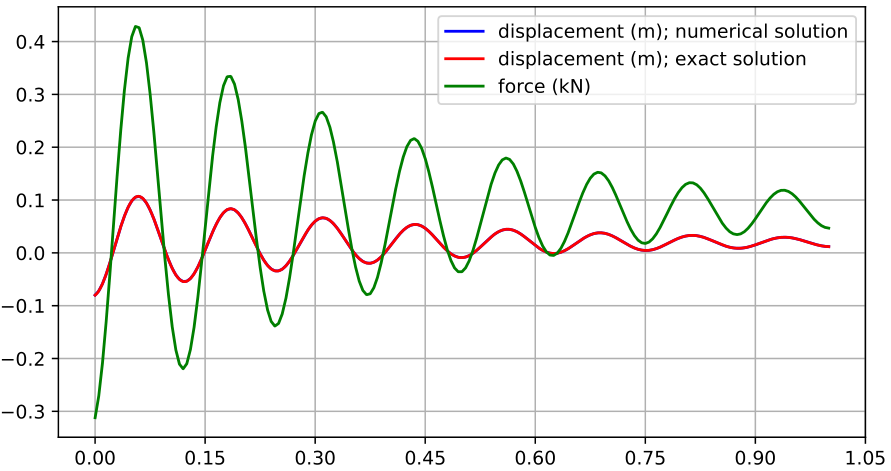
\includegraphics[height=6cm]{../demo/screenshots/plotSpringDamper}
\end{center}}
\onlyRST{

.. image:: docs/theDoc/figures/plotSpringDamper.png
   :width: 400

}
%
%\vspace{24pt}
%Further examples can be found in your copy of exudyn: 
%\bi
  %\item[] \texttt{main/pythonDev/Examples}
  %\item[] \texttt{main/pythonDev/TestModels}
%\ei



%++++++++++++++++++++++++++++++++++++++++++++++++++++++++++++++++++++++++++++++++++++++++++++++++++++++++++++++
%++++++++++++++++++++++++++++++++++++++++++++++++++++++++++++++++++++++++++++++++++++++++++++++++++++++++++++++
%++++++++++++++++++++++++++++++++++++++++++++++++++++++++++++++++++++++++++++++++++++++++++++++++++++++++++++++
\newpage
\mysubsection{Rigid body and joints tutorial}
The python source code of the first tutorial can be found in the file:
\bi
  \item[] \texttt{main/pythonDev/Examples/rigidBodyTutorial3.py}
\ei
This tutorial will set up a multibody system containing a ground, two rigid bodies and two revolute joints driven by gravity, compare a 3D view of the example in \ignoreRST{\fig{fig_RigidBodyTutorialView}.} \onlyRST{the figure above.}
\ignoreRST{\begin{figure}[tbph]
  \begin{center}
    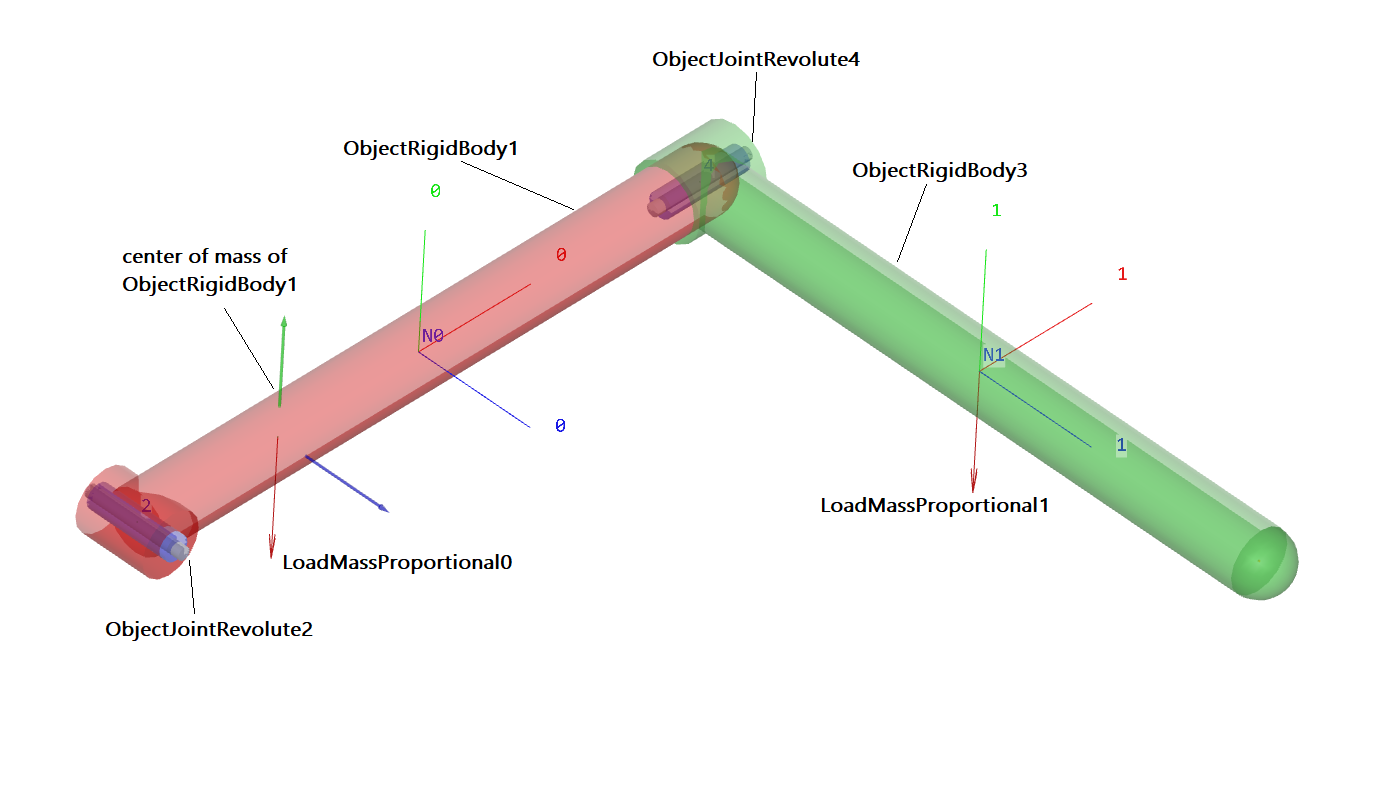
\includegraphics[width=0.9\textwidth]{figures/TutorialRigidBody1desc}
  \end{center}
  \caption{Render view of rigid body tutorial, showing objects, nodes (N0, N1), and loads.}
  \label{fig_RigidBodyTutorialView}
\end{figure}}
\onlyRST{

.. image:: docs/theDoc/figures/TutorialRigidBody1desc.png
   :width: 400

}
\horizontalRuler\\
\noindent We first import the exudyn library and the interface for all nodes, objects, markers, loads and sensors:
\pythonstyle\begin{lstlisting}
  import exudyn as exu
  from exudyn.itemInterface import *
  from exudyn.utilities import * 
  import numpy as np #for postprocessing
\end{lstlisting}
The submodule \texttt{exudyn.utilities} contains helper functions for graphics representation, 3D rigid bodies and joints.

\noindent As in the first tutorial, we need a \texttt{SystemContainer} and add a new MainSystem \texttt{mbs}:
\pythonstyle\begin{lstlisting}
  SC = exu.SystemContainer()
  mbs = SC.AddSystem()
\end{lstlisting}

\noindent We define some geometrical parameters for lateron use.
\pythonstyle\begin{lstlisting}
  #physical parameters
  g =     [0,-9.81,0] #gravity
  L = 1               #length
  w = 0.1             #width
  bodyDim=[L,w,w] #body dimensions
  p0 =    [0,0,0]     #origin of pendulum
  pMid0 = np.array([L*0.5,0,0]) #center of mass, body0
\end{lstlisting}

\noindent We add an empty ground body, using default values. It's origin is at [0,0,0] and here we use no visualization.
\pythonstyle\begin{lstlisting}
  #ground body
  oGround = mbs.AddObject(ObjectGround())
\end{lstlisting}

\horizontalRuler\\
\noindent For physical parameters of the rigid body, we can use the class \texttt{RigidBodyInertia}, which allows to define mass, center of mass (COM) and inertia parameters, as well as shifting COM or adding inertias.
The \texttt{RigidBodyInertia} can be used directly to create rigid bodies. Special derived classes can be use to define rigid body inertias for cylinders, cubes, etc., so we use a cube here:
\pythonstyle\begin{lstlisting}
  #first link:
  iCube0 = InertiaCuboid(density=5000, sideLengths=bodyDim)
  iCube0 = iCube0.Translated([-0.25*L,0,0]) #transform COM, COM not at reference point!
\end{lstlisting}
Note that the COM is translated in axial direction, while it would be at the body's local position [0,0,0] by default!

\noindent For visualization, we need to add some graphics for the body defined as a 3D RigidLink object and we additionally draw a basis (three RGB-vectors) at the COM:
\pythonstyle\begin{lstlisting}
  #graphics for body
  graphicsBody0 = GraphicsDataRigidLink(p0=[-0.5*L,0,0],p1=[0.5*L,0,0], 
                                       axis0=[0,0,1], axis1=[0,0,0], radius=[0.5*w,0.5*w], 
                                       thickness=w, width=[1.2*w,1.2*w], color=color4red)
  graphicsCOM0 = GraphicsDataBasis(origin=iCube0.com, length=2*w)
\end{lstlisting}

\noindent Now we have defined all data for the link (rigid body). We could use \texttt{mbs.AddNode(NodeRigidBodyEP(...))} and \texttt{mbs.AddObject(ObjectRigidBody(...))} to create a node and a body, but the \texttt{exudyn.rigidBodyUtilities} offer a much more comfortable function:
\pythonstyle\begin{lstlisting}
  [n0,b0]=AddRigidBody(mainSys = mbs,
                       inertia = iCube0, #includes COM
                       nodeType = exu.NodeType.RotationEulerParameters,
                       position = pMid0,
                       rotationMatrix = np.diag([1,1,1]),
                       gravity = g,
                       graphicsDataList = [graphicsBody0, graphicsCOM0])
\end{lstlisting}
which also adds a gravity load and could also set initial velocities, if wanted. 
The \texttt{nodeType} specifies the underlying model for the rigid body node, see \refSection{sec:NodeType}.
We can use 
\bi
\item \texttt{RotationEulerParameters}: for fast computation, but leads to an additional algebraic equation and thus needs an implicit solver
\item \texttt{RotationRxyz}: contains a singularity if the second angle reaches +/- 90 degrees, but no algebraic equations
\item \texttt{RotationRotationVector}: basically contains a singularity for 0 degrees, but if used in combination with Lie group integrators, singularities are bypassed
\ei

\noindent We now add a revolute joint around the (global) z-axis. 
We have several possibilities, which are shown in the following.
For the \mybold{first two possibilities only}, we need the following markers
\pythonstyle\begin{lstlisting}
  #markers for ground and rigid body (not needed for option 3):
  markerGround = mbs.AddMarker(MarkerBodyRigid(bodyNumber=oGround, localPosition=[0,0,0]))
  markerBody0J0 = mbs.AddMarker(MarkerBodyRigid(bodyNumber=b0, localPosition=[-0.5*L,0,0]))
\end{lstlisting}

\noindent The very general option 1 is to use the \texttt{GenericJoint}, that can be used to define any kind of joint with translations and rotations fixed or free,
\pythonstyle\begin{lstlisting}
  #revolute joint option 1:
  mbs.AddObject(GenericJoint(markerNumbers=[markerGround, markerBody0J0], 
                             constrainedAxes=[1,1,1,1,1,0],
                             visualization=VObjectJointGeneric(axesRadius=0.2*w, 
                                                               axesLength=1.4*w)))
\end{lstlisting}
In addition, transformation matrices (\texttt{rotationMarker0/1}) can be added, see the joint description.

\noindent Option 2 is using the revolute joint, which allows a free rotation around the local z-axis of marker 0 (\texttt{markerGround} in our example)
\pythonstyle\begin{lstlisting}
  #revolute joint option 2:
  mbs.AddObject(ObjectJointRevoluteZ(markerNumbers = [markerGround, markerBody0J0], 
                                     rotationMarker0=np.eye(3),
                                     rotationMarker1=np.eye(3),
                                     visualization=VObjectJointRevoluteZ(axisRadius=0.2*w, 
                                                                         axisLength=1.4*w)
                                     )) 
\end{lstlisting}
Additional transformation matrices (\texttt{rotationMarker0/1}) can be added in order to chose any rotation axis.

\noindent Note that an error in the definition of markers for the joints can be also detected in the render window (if you completed the example), e.g., if you change the following marker in the lines above,
\pythonstyle\begin{lstlisting}
  #example if wrong marker position is chosen:
  markerBody0J0 = mbs.AddMarker(MarkerBodyRigid(bodyNumber=b0, localPosition=[-0.4*L,0,0]))
\end{lstlisting}
$\ra$ you will see a misalignment of the two parts of the joint by \texttt{0.1*L}.

\noindent Due to the fact that the definition of markers for general joints is tedious, there is a utility function, which allows to attach revolute joints immediately to bodies and defining the rotation axis only once for the joint:
\pythonstyle\begin{lstlisting}
  #revolute joint option 3:
  AddRevoluteJoint(mbs, body0=oGround, body1=b0, point=[0,0,0], 
                   axis=[0,0,1], useGlobalFrame=True, showJoint=True,
                   axisRadius=0.2*w, axisLength=1.4*w)
\end{lstlisting}

\horizontalRuler\\
\noindent The second link and the according joint can be set up in a very similar way:
\pythonstyle\begin{lstlisting}
  #second link:
  graphicsBody1 = GraphicsDataRigidLink(p0=[0,0,-0.5*L],p1=[0,0,0.5*L], 
                                        axis0=[1,0,0], axis1=[0,0,0], radius=[0.06,0.05], 
                                        thickness = 0.1, width = [0.12,0.12], 
                                        color=color4lightgreen)

  iCube1 = InertiaCuboid(density=5000, sideLengths=[0.1,0.1,1])

  pMid1 = np.array([L,0,0]) + np.array([0,0,0.5*L]) #center of mass, body1
  [n1,b1]=AddRigidBody(mainSys = mbs,
                       inertia = iCube1,
                       nodeType = exu.NodeType.RotationEulerParameters,
                       position = pMid1,
                       rotationMatrix = np.diag([1,1,1]),
                       angularVelocity = [0,0,0],
                       gravity = g,
                       graphicsDataList = [graphicsBody1])
\end{lstlisting}

\noindent The revolute joint in this case has a free rotation around the global x-axis:
\pythonstyle\begin{lstlisting}
  #revolute joint (free x-axis)
  AddRevoluteJoint(mbs, body0=b0, body1=b1, point=[L,0,0], 
                   axis=[1,0,0], useGlobalFrame=True, showJoint=True,
                   axisRadius=0.2*w, axisLength=1.4*w)
\end{lstlisting}

\noindent Finally, we also add a sensor for some output of the double pendulum:
\pythonstyle\begin{lstlisting}
  #position sensor at tip of body1
  sens1=mbs.AddSensor(SensorBody(bodyNumber=b1, localPosition=[0,0,0.5*L],
                                 fileName='solution/sensorPos.txt',
                                 outputVariableType = exu.OutputVariableType.Position))
\end{lstlisting}
%

\horizontalRuler\\
\noindent Before simulation, we need to call \texttt{Assemble()} for our system, which links objects, nodes, ..., assigns initial values and does further pre-computations and checks:
\pythonstyle\begin{lstlisting}
  mbs.Assemble()
\end{lstlisting}
After \texttt{Assemble()}, markers, nodes, objects, etc. are linked and we can analyze the internal structure. First, we can print out useful information, either just typing \texttt{mbs} in the iPython console to print out overal information:
\plainlststyle
\begin{lstlisting}
  <systemData: 
    Number of nodes= 2
    Number of objects = 5
    Number of markers = 8
    Number of loads = 2
    Number of sensors = 1
    Number of ODE2 coordinates = 14
    Number of ODE1 coordinates = 0
    Number of AE coordinates   = 12
    Number of data coordinates   = 0

  For details see mbs.systemData, mbs.sys and mbs.variables
  >
\end{lstlisting}
%
Note that there are 2 nodes for the two rigid bodies. The five objects are due to ground object, 2 rigid bodies and 2 revolute joints.
The meaning of markers can be seen in the graphical representation described below.

Alternatively we can print the full internal information as a dictionary using:
\pythonstyle\begin{lstlisting}
  mbs.systemData.Info() #show detailed information
\end{lstlisting}
which results in the following output:
\plainlststyle
\begin{lstlisting}
  node0:
      {'nodeType': 'RigidBodyEP', 'referenceCoordinates': [0.5, 0.0, 0.0, 1.0, 0.0, 0.0, 0.0], 'addConstraintEquation': True, 'initialCoordinates': [0.0, 0.0, 0.0, 0.0, 0.0, 0.0, 0.0], 'initialVelocities': [0.0, 0.0, 0.0, 0.0, 0.0, 0.0, 0.0], 'name': 'node0', 'Vshow': True, 'VdrawSize': -1.0, 'Vcolor': [-1.0, -1.0, -1.0, -1.0]}
  node1:
      {'nodeType': 'RigidBodyEP', 'referenceCoordinates': [1.0, 0.0, 0.5, 1.0, 0.0, 0.0, 0.0], 'addConstraintEquation': True, 'initialCoordinates': [0.0, 0.0, 0.0, 0.0, 0.0, 0.0, 0.0], 'initialVelocities': [0.0, 0.0, 0.0, 0.0, 0.0, 0.0, 0.0], 'name': 'node1', 'Vshow': True, 'VdrawSize': -1.0, 'Vcolor': [-1.0, -1.0, -1.0, -1.0]}
  object0:
      {'objectType': 'Ground', 'referencePosition': [0.0, 0.0, 0.0], 'name': 'object0', 'Vshow': True, 'VgraphicsDataUserFunction': 0, 'Vcolor': [-1.0, -1.0, -1.0, -1.0], 'VgraphicsData': {'TODO': 'Get graphics data to be implemented'}}
  object1:
      {'objectType': 'RigidBody', 'physicsMass': 50.0, 'physicsInertia': [0.08333333333333336, 7.333333333333334, 7.333333333333334, 0.0, 0.0, 0.0], 'physicsCenterOfMass': [-0.25, 0.0, 0.0], 'nodeNumber': 0, 'name': 'object1', 'Vshow': True, 'VgraphicsDataUserFunction': 0, 'VgraphicsData': {'TODO': 'Get graphics data to be implemented'}}
  object2:
      {'objectType': 'JointRevolute', 'markerNumbers': [3, 4], 'rotationMarker0': [[0.0, 1.0, 0.0], [-1.0, 0.0, 0.0], [0.0, 0.0, 1.0]], 'rotationMarker1': [[0.0, 1.0, 0.0], [-1.0, 0.0, 0.0], [0.0, 0.0, 1.0]], 'activeConnector': True, 'name': 'object2', 'Vshow': True, 'VaxisRadius': 0.019999999552965164, 'VaxisLength': 0.14000000059604645, 'Vcolor': [-1.0, -1.0, -1.0, -1.0]}
  object3:
  ...
\end{lstlisting}

\noindent A graphical representation of the internal structure of the model can be shown using the command \texttt{DrawSystemGraph}:
\pythonstyle\begin{lstlisting}
  DrawSystemGraph(mbs, useItemTypes=True) #draw nice graph of system
\end{lstlisting}
For the output see \ignoreRST{\fig{fig_DrawSystemGraphExample}}\onlyRST{the figure below}. Note that obviously, markers are always needed to connect objects (or nodes) as well as loads. We can also see, that 2 markers MarkerBodyRigid1 and MarkerBodyRigid2 are unused, which is no further problem for the model and also does not require additional computational resources (except for some bytes of memory). Having isolated nodes or joints that are not connected (or having too many connections) may indicate that you did something wrong in setting up your model.
%
\ignoreRST{\begin{figure}[tbph]
  \begin{center}
    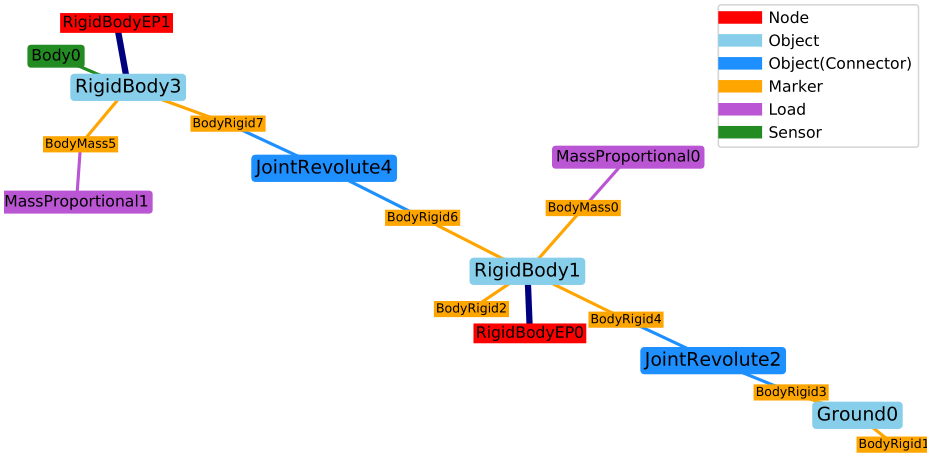
\includegraphics[width=0.9\textwidth]{figures/DrawSystemGraphExample}
  \end{center}
  \caption{System graph for rigid body tutorial. Numbers are always related to the node number, object number, etc.; note that colors are used for nodes, objects, markers, etc. $\ra$ the label names (which do not include \texttt{Object..}, \texttt{Node..}) need to be read with the color information!}
  \label{fig_DrawSystemGraphExample}
\end{figure}}
\onlyRST{

.. image:: docs/theDoc/figures/DrawSystemGraphExample.png
   :width: 400

}

\horizontalRuler\\
\noindent Before starting our simulation, we should adjust the solver parameters, especially the end time and the step size (no automatic step size for implicit solvers available!):
\pythonstyle\begin{lstlisting}
  simulationSettings = exu.SimulationSettings() #takes currently set values or default values

  tEnd = 4 #simulation time
  h = 1e-3 #step size
  simulationSettings.timeIntegration.numberOfSteps = int(tEnd/h)
  simulationSettings.timeIntegration.endTime = tEnd
  simulationSettings.timeIntegration.verboseMode = 1
  #simulationSettings.timeIntegration.simulateInRealtime = True
  simulationSettings.solutionSettings.solutionWritePeriod = 0.005 #store every 5 ms
\end{lstlisting}
The \texttt{verboseMode} tells the solver the amount of output during solving. Higher values (2, 3, ...) show residual vectors, jacobians, etc. for every time step, but slow down simulation significantly.
The option \texttt{simulateInRealtime} is used to view the model during simulation, while setting this false, the simulation finishes after fractions of a second. It should be set to false in general, while solution can be viewed using the \texttt{SolutionViewer()}.
With \texttt{solutionWritePeriod} you can adjust the frequency which is used to store the solution of the whole model, which may lead to very large files and may slow down simulation, but is used in the \texttt{SolutionViewer()} to reload the solution after simulation.

\noindent In order to improve visualization, there are hundreds of options, see Visualization settings in \refSection{sec:VSettingsGeneral}, some of them used here:
\pythonstyle\begin{lstlisting}
  SC.visualizationSettings.window.renderWindowSize=[1600,1200]
  SC.visualizationSettings.openGL.multiSampling = 4  #improved OpenGL rendering
  SC.visualizationSettings.general.autoFitScene = False

  SC.visualizationSettings.nodes.drawNodesAsPoint=False
  SC.visualizationSettings.nodes.showBasis=True #shows three RGB (=xyz) lines for node basis
\end{lstlisting}
The option \texttt{autoFitScene} is used in order to avoid zooming while loading the last saved render state, see below.

\noindent We can start the 3D visualization (Renderer) now:
\pythonstyle\begin{lstlisting}
  exu.StartRenderer()
\end{lstlisting}

\noindent In order to reload the model view of the last simulation (if there is any), we can use the following commands:
\pythonstyle\begin{lstlisting}
  if 'renderState' in exu.sys: #reload old view
      SC.SetRenderState(exu.sys['renderState'])

  mbs.WaitForUserToContinue() #stop before simulating
\end{lstlisting}
the function \texttt{WaitForUserToContinue()} waits with simulation until we press SPACE bar. This allows us to make some pre-checks.

\noindent Finally, implicit time integration (simulation) is started with:
\pythonstyle\begin{lstlisting}
  exu.SolveDynamic(mbs, simulationSettings = simulationSettings,
                   solverType=exu.DynamicSolverType.TrapezoidalIndex2)
\end{lstlisting}

\noindent After simulation, the library would immediately exit (and jump back to iPython or close the terminal window). In order to avoid this, we can use \texttt{WaitForRenderEngineStopFlag()} to wait until we press key 'Q'.
\pythonstyle\begin{lstlisting}
  SC.WaitForRenderEngineStopFlag() #stop before closing
  exu.StopRenderer() #safely close rendering window!
\end{lstlisting}
If you entered everything correctly, the render window should show a nice animation of the 3D double pendulum after pressing the SPACE key. 
If we do not stop the renderer (\texttt{StopRenderer()}), it will stay open for further simulations. However, it is safer to always close the renderer at the end.

\noindent As the simulation will run very fast, if you did not set \texttt{simulateInRealtime} to true. However, you can reload the stored solution and view the stored steps interactively:
\pythonstyle\begin{lstlisting}
  sol = LoadSolutionFile('coordinatesSolution.txt')
  from exudyn.interactive import SolutionViewer
  SolutionViewer(mbs, sol)
\end{lstlisting}

\noindent Finally, we can plot our sensor, drawing the y-component of the sensor:
\pythonstyle\begin{lstlisting}
  from exudyn.plot import PlotSensor
  PlotSensor(mbs, [sens1],[1])
\end{lstlisting}

\noindent \mybold{Congratulations}! You completed the rigid body tutorial, which gives you the ability to model multibody systems. Note that much more complicated models are possible, including feedback control or flexible bodies, see the Examples!







%+++++++++++++++++++++++++++++++++++++++++++++++++++++++++++++++++++++++++++++++
%+++++++++++++++++++++++++++++++++++++++++++++++++++++++++++++++++++++++++++++++

\mysection{Python-C++ command interface}
This section lists the basic interface functions which can be used to set up a \codeName\ model in Python.

To import the module, just include the \codeName\ module in Python (for compatibility with examples and other users, we recommend to use the 'exu' abbreviation throughout)\footnote{note that there is a second module, called exudynFast, which does deactivates all range-, index- or memory allocation checks at the gain of higher speed (probably 30 percent in regular cases). To check which version you have, just type exu.\_\_doc\_\_ and you will see a note on 'exudynFast' in the exudynFast module.}:
\bi
  \item[] \texttt{import exudyn as exu}
\ei
The exudyn module will usually hold one SystemContainer, which is a class that is initialized by assigning a system container to a variable, usually denoted as 'SC':
\bi
  \item[] \texttt{SC = exu.SystemContainer()}
\ei
Furthermore, there are a couple of commands available directly in the \codeName\ module, given in the following subsections.
Regarding the {\bf (basic) module access}, functions are related to the '\texttt{exudyn = exu}' module, see these examples:
\begin{lstlisting}[language=Python, firstnumber=14]
  import exudyn as exu
  SC = exu.SystemContainer()
  exu.InfoStat() 
  exu.Go()
  nInvalid = exu.InvalidIndex()
\end{lstlisting} \vspace{12pt}
%
Understanding the usage of functions for python object '\texttt{SystemContainer}' provided by \codeName, the following examples might help:
\begin{lstlisting}[language=Python, firstnumber=14]
  import exudyn as exu
  SC = exu.SystemContainer()
  mbs = SC.AddSystem()
  nSys = SC.NumberOfSystems()
  print(nSys)
  SC.Reset()
\end{lstlisting} \vspace{12pt}
%
Understanding the usage of functions for the '\texttt{MainSystem}' provided by \texttt{SystemContainer}, the following examples might help:
\begin{lstlisting}[language=Python, firstnumber=14]
  import exudyn as exu
  SC = exu.SystemContainer()
  mbs = SC.AddSystem()
  mbs.Reset()
  mbs.WaitForUserToContinue() 
\end{lstlisting} \vspace{12pt}
%

% ++++++++++++++++++++++% description of manual pybind interfaces; generated by Johannes Gerstmayr% ++++++++++++++++++++++
%++++++++++++++++++++
\mysubsection{\codeName}
These are the access functions to the \codeName\ module.

\begin{center}
\footnotesize
\begin{longtable}{| p{8cm} | p{8cm} |} 
\hline
{\bf function/structure name} & {\bf description}\\ \hline
  GetVersionString() & Get EXUDYN module version as string\\ \hline 
  RequireVersion(requiredVersionString) & Checks if the installed version is according to the required version. Major, micro and minor version must agree the required level. Example: RequireVersion("1.0.31")\\ \hline 
  StartRenderer(verbose = false) & Start OpenGL rendering engine (in separate thread); use verbose=True to output information during OpenGL window creation; some of the information will only be seen in windows command (powershell) windows or linux shell, but not inside iPython of Spyder\\ \hline 
  StopRenderer() & Stop OpenGL rendering engine\\ \hline 
  DoRendererIdleTasks(waitSeconds = 0) & Call this function in order to interact with Renderer window; use waitSeconds in order to run this idle tasks while animating a model (e.g. waitSeconds=0.04), use waitSeconds=0 without waiting, or use waitSeconds=-1 to wait until window is closed\\ \hline 
  SolveStatic(mbs, simulationSettings = exudyn.SimulationSettings(), updateInitialValues = False, storeSolver = True) & Static solver function, mapped from module \texttt{solver}; for details on the python interface see \refSection{sec:solver:SolveStatic}; for background on solvers, see \refSection{sec:solvers}\\ \hline 
  SolveDynamic(mbs, simulationSettings = exudyn.SimulationSettings(), solverType = exudyn.DynamicSolverType.GeneralizedAlpha, updateInitialValues = False, storeSolver = True) & Dynamic solver function, mapped from module \texttt{solver}; for details on the python interface see \refSection{sec:solver:SolveDynamic}; for background on solvers, see \refSection{sec:solvers}\\ \hline 
  ComputeODE2Eigenvalues(mbs, simulationSettings = exudyn.SimulationSettings(), useSparseSolver = False, numberOfEigenvalues = -1, setInitialValues = True, convert2Frequencies = False) & Simple interface to scipy eigenvalue solver for eigenvalue analysis of the second order differential equations part in mbs, mapped from module \texttt{solver}; for details on the python interface see \refSection{sec:solver:ComputeODE2Eigenvalues}\\ \hline 
  SetOutputPrecision(numberOfDigits) & Set the precision (integer) for floating point numbers written to console (reset when simulation is started!)\\ \hline 
  SetLinalgOutputFormatPython(flagPythonFormat) & true: use python format for output of vectors and matrices; false: use matlab format\\ \hline 
  SetWriteToConsole(flag) & set flag to write (true) or not write to console; default = true\\ \hline 
  SetWriteToFile(filename, flagWriteToFile = true, flagAppend = false) & set flag to write (true) or not write to console; default value of flagWriteToFile = false; flagAppend appends output to file, if set true; in order to finalize the file, write exu.SetWriteToFile('', False) to close the output file\tabnewline 
    \textcolor{steelblue}{{\bf EXAMPLE}: \tabnewline 
    \texttt{exu.SetWriteToConsole(False) \#no output to console\tabnewline
    exu.SetWriteToFile(filename={\textquotesingle}testOutput.log{\textquotesingle}, flagWriteToFile=True, flagAppend=False)\tabnewline
    exu.Print({\textquotesingle}print this to file{\textquotesingle})\tabnewline
    exu.SetWriteToFile({\textquotesingle}{\textquotesingle}, False) \#terminate writing to file which closes the file}}\\ \hline 
  SetPrintDelayMilliSeconds(delayMilliSeconds) & add some delay (in milliSeconds) to printing to console, in order to let Spyder process the output; default = 0\\ \hline 
  Print() & this allows printing via exudyn with similar syntax as in python print(args) except for keyword arguments: print('test=',42); allows to redirect all output to file given by SetWriteToFile(...); does not output in case that SetWriteToConsole is set to false\\ \hline 
  InfoStat(writeOutput = true) & Retrieve list of global information on memory allocation and other counts as list:[array\_new\_counts, array\_delete\_counts, vector\_new\_counts, vector\_delete\_counts, matrix\_new\_counts, matrix\_delete\_counts, linkedDataVectorCast\_counts]; May be extended in future; if writeOutput==True, it additionally prints the statistics; counts for new vectors and matrices should not depend on numberOfSteps, except for some objects such as ObjectGenericODE2 and for (sensor) output to files; Not available if code is compiled with \_\_FAST\_EXUDYN\_LINALG flag\\ \hline 
  Go() & Creates a SystemContainer SC and a main system mbs\\ \hline 
  InvalidIndex() & This function provides the invalid index, which may depend on the kind of 32-bit, 64-bit signed or unsigned integer; e.g. node index or item index in list; currently, the InvalidIndex() gives -1, but it may be changed in future versions, therefore you should use this function\\ \hline 
  variables & this dictionary may be used by the user to store exudyn-wide data in order to avoid global python variables; usage: exu.variables["myvar"] = 42 \\ \hline  
  sys & this dictionary is used and reserved by the system, e.g. for testsuite, graphics or system function to store module-wide data in order to avoid global python variables; the variable exu.sys['renderState'] contains the last render state after exu.StopRenderer() and can be used for subsequent simulations \\ \hline  
\end{longtable}
\end{center}

%++++++++++++++++++++
\mysubsection{SystemContainer}
The SystemContainer is the top level of structures in \codeName. The container holds all systems, solvers and all other data structures for computation. Currently, only one container shall be used. In future, multiple containers might be usable at the same time. \\ Example: \\ \texttt{import exudyn as exu \\ SC = exu.SystemContainer() \\ mbs = SC.AddSystem()}

\begin{center}
\footnotesize
\begin{longtable}{| p{8cm} | p{8cm} |} 
\hline
{\bf function/structure name} & {\bf description}\\ \hline
  Reset() & delete all systems and reset SystemContainer (including graphics); this also releases SystemContainer from the renderer, which requires SC.AttachToRenderEngine() to be called in order to reconnect to rendering; a safer way is to delete the current SystemContainer and create a new one (SC=SystemContainer() )\\ \hline 
  AddSystem() & add a new computational system\\ \hline 
  NumberOfSystems() & obtain number of systems available in system container\\ \hline 
  GetSystem(systemNumber) & obtain systems with index from system container\\ \hline 
  visualizationSettings & this structure is read/writeable and contains visualization settings, which are immediately applied to the rendering window. \tabnewline
    EXAMPLE:\tabnewline
    SC = exu.SystemContainer()\tabnewline
    SC.visualizationSettings.autoFitScene=False  \\ \hline  
  GetRenderState() & Get dictionary with current render state (openGL zoom, modelview, etc.); will have no effect if GLFW\_GRAPHICS is deactivated\tabnewline 
    \textcolor{steelblue}{{\bf EXAMPLE}: \tabnewline 
    \texttt{SC = exu.SystemContainer()\tabnewline
    renderState = SC.GetRenderState() \tabnewline
    print(renderState[{\textquotesingle}zoom{\textquotesingle}])}}\\ \hline 
  SetRenderState(renderState) & Set current render state (openGL zoom, modelview, etc.) with given dictionary; usually, this dictionary has been obtained with GetRenderState; will have no effect if GLFW\_GRAPHICS is deactivated\tabnewline 
    \textcolor{steelblue}{{\bf EXAMPLE}: \tabnewline 
    \texttt{SC = exu.SystemContainer()\tabnewline
    SC.SetRenderState(renderState)}}\\ \hline 
  RedrawAndSaveImage() & Redraw openGL scene and save image (command waits until process is finished)\\ \hline 
  WaitForRenderEngineStopFlag() & Wait for user to stop render engine (Press 'Q' or Escape-key)\\ \hline 
  RenderEngineZoomAll() & Send zoom all signal, which will perform zoom all at next redraw request\\ \hline 
  RedrawAndSaveImage() & Redraw openGL scene and save image (command waits until process is finished)\\ \hline 
  AttachToRenderEngine() & Links the SystemContainer to the render engine, such that the changes in the graphics structure drawn upon updates, etc.; done automatically on creation of SystemContainer; return False, if no renderer exists (e.g., compiled without GLFW) or cannot be linked (if other SystemContainer already linked)\\ \hline 
  DetachFromRenderEngine() & Releases the SystemContainer from the render engine; return True if successfully released, False if no GLFW available or detaching failed\\ \hline 
  GetCurrentMouseCoordinates(useOpenGLcoordinates = False) & Get current mouse coordinates as list [x, y]; x and y being floats, as returned by GLFW, measured from top left corner of window; use GetCurrentMouseCoordinates(useOpenGLcoordinates=True) to obtain OpenGLcoordinates of projected plane\\ \hline 
\end{longtable}
\end{center}

%++++++++++++++++++++
\mysubsection{MainSystem}
This is the structure which defines a (multibody) system. In C++, there is a MainSystem (links to python) and a System (computational part). For that reason, the name is MainSystem on the python side, but it is often just called 'system'. It can be created, visualized and computed. Use the following functions for system manipulation. \\ \\ Usage: \\ \\ \texttt{import exudyn as exu \\ SC = exu.SystemContainer() \\ mbs = SC.AddSystem()}

\begin{center}
\footnotesize
\begin{longtable}{| p{8cm} | p{8cm} |} 
\hline
{\bf function/structure name} & {\bf description}\\ \hline
  Assemble() & assemble items (nodes, bodies, markers, loads, ...); Calls CheckSystemIntegrity(...), AssembleCoordinates(), AssembleLTGLists(), and AssembleInitializeSystemCoordinates()\\ \hline 
  AssembleCoordinates() & assemble coordinates: assign computational coordinates to nodes and constraints (algebraic variables)\\ \hline 
  AssembleLTGLists() & build local-to-global (ltg) coordinate lists for objects (used to build global ODE2RHS, MassMatrix, etc. vectors and matrices) and store special object lists (body, connector, constraint, ...)\\ \hline 
  AssembleInitializeSystemCoordinates() & initialize all system-wide coordinates based on initial values given in nodes\\ \hline 
  Reset() & reset all lists of items (nodes, bodies, markers, loads, ...) and temporary vectors; deallocate memory\\ \hline 
  GetSystemContainer() & return the systemContainer where the mainSystem (mbs) was created\\ \hline 
  WaitForUserToContinue() & interrupt further computation until user input --> 'pause' function\\ \hline 
  SendRedrawSignal() & this function is used to send a signal to the renderer that the scene shall be redrawn because the visualization state has been updated\\ \hline 
  GetRenderEngineStopFlag() & get the current stop simulation flag; true=user wants to stop simulation\\ \hline 
  SetRenderEngineStopFlag() & set the current stop simulation flag; set to false, in order to continue a previously user-interrupted simulation\\ \hline 
  ActivateRendering(flag = true) & activate (flag=True) or deactivate (flag=False) rendering for this system\\ \hline 
  SetPreStepUserFunction() & Sets a user function PreStepUserFunction(mbs, t) executed at beginning of every computation step; in normal case return True; return False to stop simulation after current step\tabnewline 
    \textcolor{steelblue}{{\bf EXAMPLE}: \tabnewline 
    \texttt{def PreStepUserFunction(mbs, t):\tabnewline
     \phantom{XXXX} print(mbs.systemData.NumberOfNodes())\tabnewline
     \phantom{XXXX} if(t>1): \tabnewline
     \phantom{XXXX} \phantom{XXXX} return False \tabnewline
     \phantom{XXXX} return True \tabnewline
     mbs.SetPreStepUserFunction(PreStepUserFunction)}}\\ \hline 
  SetPostNewtonUserFunction() & Sets a user function PostNewtonUserFunction(mbs, t) executed after successful Newton iteration in implicit or static solvers and after step update of explicit solvers, but BEFORE PostNewton functions are called by the solver; function returns list [discontinuousError, recommendedStepSize], containing a error of the PostNewtonStep, which is compared to [solver].discontinuous.iterationTolerance. The recommendedStepSize shall be negative, if no recommendation is given, 0 in order to enforce minimum step size or a specific value to which the current step size will be reduced and the step will be repeated; use this function, e.g., to reduce step size after impact or change of data variables\tabnewline 
    \textcolor{steelblue}{{\bf EXAMPLE}: \tabnewline 
    \texttt{def PostNewtonUserFunction(mbs, t):\tabnewline
     \phantom{XXXX} if(t>1): \tabnewline
     \phantom{XXXX} \phantom{XXXX} return [0, 1e-6] \tabnewline
     \phantom{XXXX} return [0,0] \tabnewline
     mbs.SetPostNewtonUserFunction(PostNewtonUserFunction)}}\\ \hline 
  \_\_repr\_\_() & return the representation of the system, which can be, e.g., printed\tabnewline 
    \textcolor{steelblue}{{\bf EXAMPLE}: \tabnewline 
    \texttt{print(mbs)}}\\ \hline 
  systemIsConsistent & this flag is used by solvers to decide, whether the system is in a solvable state; this flag is set to false as long as Assemble() has not been called; any modification to the system, such as Add...(), Modify...(), etc. will set the flag to false again; this flag can be modified (set to true), if a change of e.g.~an object (change of stiffness) or load (change of force) keeps the system consistent, but would normally lead to systemIsConsistent=False  \\ \hline  
  interactiveMode & set this flag to true in order to invoke a Assemble() command in every system modification, e.g. AddNode, AddObject, ModifyNode, ...; this helps that the system can be visualized in interactive mode. \\ \hline  
  variables & this dictionary may be used by the user to store model-specific data, in order to avoid global python variables in complex models; mbs.variables["myvar"] = 42 \\ \hline  
  sys & this dictionary is used by exudyn python libraries, e.g., solvers, to avoid global python variables \\ \hline 
  solverSignalJacobianUpdate & this flag is used by solvers to decide, whether the jacobian should be updated; at beginning of simulation and after jacobian computation, this flag is set automatically to False; use this flag to indicate system changes, e.g. during time integration  \\ \hline  
  systemData & Access to SystemData structure; enables access to number of nodes, objects, ... and to (current, initial, reference, ...) state variables (ODE2, AE, Data,...)\\ \hline  
\end{longtable}
\end{center}

%++++++++++++++++++++
\mysubsubsection{MainSystem: Node}
\label{sec:mainsystem:node}
 This section provides functions for adding, reading and modifying nodes. Nodes are used to define coordinates (unknowns to the static system and degrees of freedom if constraints are not present). Nodes can provide various types of coordinates for second/first order differential equations (ODE2/ODE1), algebraic equations (AE) and for data (history) variables -- which are not providing unknowns in the nonlinear solver but will be solved in an additional nonlinear iteration for e.g. contact, friction or plasticity.

\begin{center}
\footnotesize
\begin{longtable}{| p{8cm} | p{8cm} |} 
\hline
{\bf function/structure name} & {\bf description}\\ \hline
  AddNode(pyObject) & add a node with nodeDefinition from Python node class; returns (global) node index (type NodeIndex) of newly added node; use int(nodeIndex) to convert to int, if needed (but not recommended in order not to mix up index types of nodes, objects, markers, ...)\tabnewline 
    \textcolor{steelblue}{{\bf EXAMPLE}: \tabnewline 
    \texttt{item = Rigid2D( referenceCoordinates= [1,0.5,0], initialVelocities= [10,0,0]) \tabnewline
    mbs.AddNode(item) \tabnewline
    nodeDict = \{{\textquotesingle}nodeType{\textquotesingle}: {\textquotesingle}Point{\textquotesingle}, \tabnewline
    {\textquotesingle}referenceCoordinates{\textquotesingle}: [1.0, 0.0, 0.0], \tabnewline
    {\textquotesingle}initialCoordinates{\textquotesingle}: [0.0, 2.0, 0.0], \tabnewline
    {\textquotesingle}name{\textquotesingle}: {\textquotesingle}example node{\textquotesingle}\} \tabnewline
     mbs.AddNode(nodeDict)}}\\ \hline 
  GetNodeNumber(nodeName) & get node's number by name (string)\tabnewline 
    \textcolor{steelblue}{{\bf EXAMPLE}: \tabnewline 
    \texttt{n = mbs.GetNodeNumber({\textquotesingle}example node{\textquotesingle})}}\\ \hline 
  GetNode(nodeNumber) & get node's dictionary by node number (type NodeIndex)\tabnewline 
    \textcolor{steelblue}{{\bf EXAMPLE}: \tabnewline 
    \texttt{nodeDict = mbs.GetNode(0)}}\\ \hline 
  ModifyNode(nodeNumber, nodeDict) & modify node's dictionary by node number (type NodeIndex)\tabnewline 
    \textcolor{steelblue}{{\bf EXAMPLE}: \tabnewline 
    \texttt{mbs.ModifyNode(nodeNumber, nodeDict)}}\\ \hline 
  GetNodeDefaults(typeName) & get node's default values for a certain nodeType as (dictionary)\tabnewline 
    \textcolor{steelblue}{{\bf EXAMPLE}: \tabnewline 
    \texttt{nodeType = {\textquotesingle}Point{\textquotesingle}\tabnewline
    nodeDict = mbs.GetNodeDefaults(nodeType)}}\\ \hline 
  GetNodeOutput(nodeNumber, variableType, configuration = ConfigurationType.Current) & get the ouput of the node specified with the OutputVariableType; default configuration = 'current'; output may be scalar or array (e.g. displacement vector)\tabnewline 
    \textcolor{steelblue}{{\bf EXAMPLE}: \tabnewline 
    \texttt{mbs.GetNodeOutput(nodeNumber=0, variableType=exu.OutputVariableType.Displacement)}}\\ \hline 
  GetNodeODE2Index(nodeNumber) & get index in the global ODE2 coordinate vector for the first node coordinate of the specified node\tabnewline 
    \textcolor{steelblue}{{\bf EXAMPLE}: \tabnewline 
    \texttt{mbs.GetNodeODE2Index(nodeNumber=0)}}\\ \hline 
  GetNodeParameter(nodeNumber, parameterName) & get nodes's parameter from node number (type NodeIndex) and parameterName; parameter names can be found for the specific items in the reference manual\\ \hline 
  SetNodeParameter(nodeNumber, parameterName, value) & set parameter 'parameterName' of node with node number (type NodeIndex) to value; parameter names can be found for the specific items in the reference manual\\ \hline 
\end{longtable}
\end{center}

%++++++++++++++++++++
\mysubsubsection{MainSystem: Object}
\label{sec:mainsystem:object}
 This section provides functions for adding, reading and modifying objects, which can be bodies (mass point, rigid body, finite element, ...), connectors (spring-damper or joint) or general objects. Objects provided terms to the residual of equations resulting from every coordinate given by the nodes. Single-noded objects (e.g.~mass point) provides exactly residual terms for its nodal coordinates. Connectors constrain or penalize two markers, which can be, e.g., position, rigid or coordinate markers. Thus, the dependence of objects is either on the coordinates of the marker-objects/nodes or on nodes which the objects possess themselves.

\begin{center}
\footnotesize
\begin{longtable}{| p{8cm} | p{8cm} |} 
\hline
{\bf function/structure name} & {\bf description}\\ \hline
  AddObject(pyObject) & add an object with objectDefinition from Python object class; returns (global) object number (type ObjectIndex) of newly added object\tabnewline 
    \textcolor{steelblue}{{\bf EXAMPLE}: \tabnewline 
    \texttt{item = MassPoint(name={\textquotesingle}heavy object{\textquotesingle}, nodeNumber=0, physicsMass=100) \tabnewline
    mbs.AddObject(item) \tabnewline
    objectDict = \{{\textquotesingle}objectType{\textquotesingle}: {\textquotesingle}MassPoint{\textquotesingle}, \tabnewline
    {\textquotesingle}physicsMass{\textquotesingle}: 10, \tabnewline
    {\textquotesingle}nodeNumber{\textquotesingle}: 0, \tabnewline
    {\textquotesingle}name{\textquotesingle}: {\textquotesingle}example object{\textquotesingle}\} \tabnewline
     mbs.AddObject(objectDict)}}\\ \hline 
  GetObjectNumber(objectName) & get object's number by name (string)\tabnewline 
    \textcolor{steelblue}{{\bf EXAMPLE}: \tabnewline 
    \texttt{n = mbs.GetObjectNumber({\textquotesingle}heavy object{\textquotesingle})}}\\ \hline 
  GetObject(objectNumber) & get object's dictionary by object number (type ObjectIndex)\tabnewline 
    \textcolor{steelblue}{{\bf EXAMPLE}: \tabnewline 
    \texttt{objectDict = mbs.GetObject(0)}}\\ \hline 
  ModifyObject(objectNumber, objectDict) & modify object's dictionary by object number (type ObjectIndex)\tabnewline 
    \textcolor{steelblue}{{\bf EXAMPLE}: \tabnewline 
    \texttt{mbs.ModifyObject(objectNumber, objectDict)}}\\ \hline 
  GetObjectDefaults(typeName) & get object's default values for a certain objectType as (dictionary)\tabnewline 
    \textcolor{steelblue}{{\bf EXAMPLE}: \tabnewline 
    \texttt{objectType = {\textquotesingle}MassPoint{\textquotesingle}\tabnewline
    objectDict = mbs.GetObjectDefaults(objectType)}}\\ \hline 
  GetObjectOutput(objectNumber, variableType) & get object's current output variable from object number (type ObjectIndex) and OutputVariableType; can only be computed for exu.ConfigurationType.Current configuration!\\ \hline 
  GetObjectOutputBody(objectNumber, variableType, localPosition, configuration = ConfigurationType.Current) & get body's output variable from object number (type ObjectIndex) and OutputVariableType, using the localPosition $\pLocB$ similar to MarkerBody and SensorBody\tabnewline 
    \textcolor{steelblue}{{\bf EXAMPLE}: \tabnewline 
    \texttt{u = mbs.GetObjectOutputBody(objectNumber = 1, variableType = exu.OutputVariableType.Position, localPosition=[1,0,0], configuration = exu.ConfigurationType.Initial)}}\\ \hline 
  GetObjectOutputSuperElement(objectNumber, variableType, meshNodeNumber, configuration = ConfigurationType.Current) & get output variable from mesh node number of object with type SuperElement (GenericODE2, FFRF, FFRFreduced - CMS) with specific OutputVariableType; the meshNodeNumber is the object's local node number, not the global node number!\tabnewline 
    \textcolor{steelblue}{{\bf EXAMPLE}: \tabnewline 
    \texttt{u = mbs.GetObjectOutputSuperElement(objectNumber = 1, variableType = exu.OutputVariableType.Position, meshNodeNumber = 12, configuration = exu.ConfigurationType.Initial)}}\\ \hline 
  GetObjectParameter(objectNumber, parameterName) & get objects's parameter from object number (type ObjectIndex) and parameterName; parameter names can be found for the specific items in the reference manual\\ \hline 
  SetObjectParameter(objectNumber, parameterName, value) & set parameter 'parameterName' of object with object number (type ObjectIndex) to value; parameter names can be found for the specific items in the reference manual\\ \hline 
\end{longtable}
\end{center}

%++++++++++++++++++++
\mysubsubsection{MainSystem: Marker}
\label{sec:mainsystem:marker}
 This section provides functions for adding, reading and modifying markers. Markers define how to measure primal kinematical quantities on objects or nodes (e.g., position, orientation or coordinates themselves), and how to act on the quantities which are dual to the kinematical quantities (e.g., force, torque and generalized forces). Markers provide unique interfaces for loads, sensors and constraints in order to address these quantities independently of the structure of the object or node (e.g., rigid or flexible body).

\begin{center}
\footnotesize
\begin{longtable}{| p{8cm} | p{8cm} |} 
\hline
{\bf function/structure name} & {\bf description}\\ \hline
  AddMarker(pyObject) & add a marker with markerDefinition from Python marker class; returns (global) marker number (type MarkerIndex) of newly added marker\tabnewline 
    \textcolor{steelblue}{{\bf EXAMPLE}: \tabnewline 
    \texttt{item = MarkerNodePosition(name={\textquotesingle}my marker{\textquotesingle},nodeNumber=1) \tabnewline
    mbs.AddMarker(item)\tabnewline
    markerDict = \{{\textquotesingle}markerType{\textquotesingle}: {\textquotesingle}NodePosition{\textquotesingle}, \tabnewline
     {\textquotesingle}nodeNumber{\textquotesingle}: 0, \tabnewline
     {\textquotesingle}name{\textquotesingle}: {\textquotesingle}position0{\textquotesingle}\}\tabnewline
     mbs.AddMarker(markerDict)}}\\ \hline 
  GetMarkerNumber(markerName) & get marker's number by name (string)\tabnewline 
    \textcolor{steelblue}{{\bf EXAMPLE}: \tabnewline 
    \texttt{n = mbs.GetMarkerNumber({\textquotesingle}my marker{\textquotesingle})}}\\ \hline 
  GetMarker(markerNumber) & get marker's dictionary by index\tabnewline 
    \textcolor{steelblue}{{\bf EXAMPLE}: \tabnewline 
    \texttt{markerDict = mbs.GetMarker(0)}}\\ \hline 
  ModifyMarker(markerNumber, markerDict) & modify marker's dictionary by index\tabnewline 
    \textcolor{steelblue}{{\bf EXAMPLE}: \tabnewline 
    \texttt{mbs.ModifyMarker(markerNumber, markerDict)}}\\ \hline 
  GetMarkerDefaults(typeName) & get marker's default values for a certain markerType as (dictionary)\tabnewline 
    \textcolor{steelblue}{{\bf EXAMPLE}: \tabnewline 
    \texttt{markerType = {\textquotesingle}NodePosition{\textquotesingle}\tabnewline
    markerDict = mbs.GetMarkerDefaults(markerType)}}\\ \hline 
  GetMarkerParameter(markerNumber, parameterName) & get markers's parameter from markerNumber and parameterName; parameter names can be found for the specific items in the reference manual\\ \hline 
  SetMarkerParameter(markerNumber, parameterName, value) & set parameter 'parameterName' of marker with markerNumber to value; parameter names can be found for the specific items in the reference manual\\ \hline 
\end{longtable}
\end{center}

%++++++++++++++++++++
\mysubsubsection{MainSystem: Load}
\label{sec:mainsystem:load}
 This section provides functions for adding, reading and modifying operating loads. Loads are used to act on the quantities which are dual to the primal kinematic quantities, such as displacement and rotation. Loads represent, e.g., forces, torques or generalized forces.

\begin{center}
\footnotesize
\begin{longtable}{| p{8cm} | p{8cm} |} 
\hline
{\bf function/structure name} & {\bf description}\\ \hline
  AddLoad(pyObject) & add a load with loadDefinition from Python load class; returns (global) load number (type LoadIndex) of newly added load\tabnewline 
    \textcolor{steelblue}{{\bf EXAMPLE}: \tabnewline 
    \texttt{item = mbs.AddLoad(LoadForceVector(loadVector=[1,0,0], markerNumber=0, name={\textquotesingle}heavy load{\textquotesingle})) \tabnewline
    mbs.AddLoad(item)\tabnewline
    loadDict = \{{\textquotesingle}loadType{\textquotesingle}: {\textquotesingle}ForceVector{\textquotesingle},\tabnewline
     {\textquotesingle}markerNumber{\textquotesingle}: 0,\tabnewline
     {\textquotesingle}loadVector{\textquotesingle}: [1.0, 0.0, 0.0],\tabnewline
     {\textquotesingle}name{\textquotesingle}: {\textquotesingle}heavy load{\textquotesingle}\} \tabnewline
     mbs.AddLoad(loadDict)}}\\ \hline 
  GetLoadNumber(loadName) & get load's number by name (string)\tabnewline 
    \textcolor{steelblue}{{\bf EXAMPLE}: \tabnewline 
    \texttt{n = mbs.GetLoadNumber({\textquotesingle}heavy load{\textquotesingle})}}\\ \hline 
  GetLoad(loadNumber) & get load's dictionary by index\tabnewline 
    \textcolor{steelblue}{{\bf EXAMPLE}: \tabnewline 
    \texttt{loadDict = mbs.GetLoad(0)}}\\ \hline 
  ModifyLoad(loadNumber, loadDict) & modify load's dictionary by index\tabnewline 
    \textcolor{steelblue}{{\bf EXAMPLE}: \tabnewline 
    \texttt{mbs.ModifyLoad(loadNumber, loadDict)}}\\ \hline 
  GetLoadDefaults(typeName) & get load's default values for a certain loadType as (dictionary)\tabnewline 
    \textcolor{steelblue}{{\bf EXAMPLE}: \tabnewline 
    \texttt{loadType = {\textquotesingle}ForceVector{\textquotesingle}\tabnewline
    loadDict = mbs.GetLoadDefaults(loadType)}}\\ \hline 
  GetLoadValues(loadNumber) & Get current load values, specifically if user-defined loads are used; can be scalar or vector-valued return value\\ \hline 
  GetLoadParameter(loadNumber, parameterName) & get loads's parameter from loadNumber and parameterName; parameter names can be found for the specific items in the reference manual\\ \hline 
  SetLoadParameter(loadNumber, parameterName, value) & set parameter 'parameterName' of load with loadNumber to value; parameter names can be found for the specific items in the reference manual\\ \hline 
\end{longtable}
\end{center}

%++++++++++++++++++++
\mysubsubsection{MainSystem: Sensor}
\label{sec:mainsystem:sensor}
 This section provides functions for adding, reading and modifying operating sensors. Sensors are used to measure information in nodes, objects, markers, and loads for output in a file.

\begin{center}
\footnotesize
\begin{longtable}{| p{8cm} | p{8cm} |} 
\hline
{\bf function/structure name} & {\bf description}\\ \hline
  AddSensor(pyObject) & add a sensor with sensor definition from Python sensor class; returns (global) sensor number (type SensorIndex) of newly added sensor\tabnewline 
    \textcolor{steelblue}{{\bf EXAMPLE}: \tabnewline 
    \texttt{item = mbs.AddSensor(SensorNode(sensorType= exu.SensorType.Node, nodeNumber=0, name={\textquotesingle}test sensor{\textquotesingle})) \tabnewline
    mbs.AddSensor(item)\tabnewline
    sensorDict = \{{\textquotesingle}sensorType{\textquotesingle}: {\textquotesingle}Node{\textquotesingle},\tabnewline
     {\textquotesingle}nodeNumber{\textquotesingle}: 0,\tabnewline
     {\textquotesingle}fileName{\textquotesingle}: {\textquotesingle}sensor.txt{\textquotesingle},\tabnewline
     {\textquotesingle}name{\textquotesingle}: {\textquotesingle}test sensor{\textquotesingle}\} \tabnewline
     mbs.AddSensor(sensorDict)}}\\ \hline 
  GetSensorNumber(sensorName) & get sensor's number by name (string)\tabnewline 
    \textcolor{steelblue}{{\bf EXAMPLE}: \tabnewline 
    \texttt{n = mbs.GetSensorNumber({\textquotesingle}test sensor{\textquotesingle})}}\\ \hline 
  GetSensor(sensorNumber) & get sensor's dictionary by index\tabnewline 
    \textcolor{steelblue}{{\bf EXAMPLE}: \tabnewline 
    \texttt{sensorDict = mbs.GetSensor(0)}}\\ \hline 
  ModifySensor(sensorNumber, sensorDict) & modify sensor's dictionary by index\tabnewline 
    \textcolor{steelblue}{{\bf EXAMPLE}: \tabnewline 
    \texttt{mbs.ModifySensor(sensorNumber, sensorDict)}}\\ \hline 
  GetSensorDefaults(typeName) & get sensor's default values for a certain sensorType as (dictionary)\tabnewline 
    \textcolor{steelblue}{{\bf EXAMPLE}: \tabnewline 
    \texttt{sensorType = {\textquotesingle}Node{\textquotesingle}\tabnewline
    sensorDict = mbs.GetSensorDefaults(sensorType)}}\\ \hline 
  GetSensorValues(sensorNumber, configuration = ConfigurationType.Current) & get sensors's values for configuration; can be a scalar or vector-valued return value!\\ \hline 
  GetSensorParameter(sensorNumber, parameterName) & get sensors's parameter from sensorNumber and parameterName; parameter names can be found for the specific items in the reference manual\\ \hline 
  SetSensorParameter(sensorNumber, parameterName, value) & set parameter 'parameterName' of sensor with sensorNumber to value; parameter names can be found for the specific items in the reference manual\\ \hline 
\end{longtable}
\end{center}

%++++++++++++++++++++
\mysubsection{SystemData}
This is the data structure of a system which contains Objects (bodies/constraints/...), Nodes, Markers and Loads. The SystemData structure allows advanced access to this data, which HAS TO BE USED WITH CARE, as unexpected results and system crash might happen. \\ 
 Usage: \\ \small 
\texttt{\#obtain current ODE2 system vector (e.g. after static simulation finished): \\ u = mbs.systemData.GetODE2Coordinates() \\ \#set initial ODE2 vector for next simulation:\\ 
mbs.systemData.SetODE2Coordinates(coordinates=u,configurationType=exu.ConfigurationType.Initial)}


\begin{center}
\footnotesize
\begin{longtable}{| p{8cm} | p{8cm} |} 
\hline
{\bf function/structure name} & {\bf description}\\ \hline
  NumberOfLoads() & return number of loads in system\tabnewline 
    \textcolor{steelblue}{{\bf EXAMPLE}: \tabnewline 
    \texttt{print(mbs.systemData.NumberOfLoads())}}\\ \hline 
  NumberOfMarkers() & return number of markers in system\tabnewline 
    \textcolor{steelblue}{{\bf EXAMPLE}: \tabnewline 
    \texttt{print(mbs.systemData.NumberOfMarkers())}}\\ \hline 
  NumberOfNodes() & return number of nodes in system\tabnewline 
    \textcolor{steelblue}{{\bf EXAMPLE}: \tabnewline 
    \texttt{print(mbs.systemData.NumberOfNodes())}}\\ \hline 
  NumberOfObjects() & return number of objects in system\tabnewline 
    \textcolor{steelblue}{{\bf EXAMPLE}: \tabnewline 
    \texttt{print(mbs.systemData.NumberOfObjects())}}\\ \hline 
  NumberOfSensors() & return number of sensors in system\tabnewline 
    \textcolor{steelblue}{{\bf EXAMPLE}: \tabnewline 
    \texttt{print(mbs.systemData.NumberOfSensors())}}\\ \hline 
  ODE2Size(configurationType = exu.ConfigurationType.Current) & get size of ODE2 coordinate vector for given configuration (only works correctly after mbs.Assemble() )\tabnewline 
    \textcolor{steelblue}{{\bf EXAMPLE}: \tabnewline 
    \texttt{print({\textquotesingle}ODE2 size={\textquotesingle},mbs.systemData.ODE2Size())}}\\ \hline 
  ODE1Size(configurationType = exu.ConfigurationType.Current) & get size of ODE1 coordinate vector for given configuration (only works correctly after mbs.Assemble() )\tabnewline 
    \textcolor{steelblue}{{\bf EXAMPLE}: \tabnewline 
    \texttt{print({\textquotesingle}ODE1 size={\textquotesingle},mbs.systemData.ODE1Size())}}\\ \hline 
  AEsize(configurationType = exu.ConfigurationType.Current) & get size of AE coordinate vector for given configuration (only works correctly after mbs.Assemble() )\tabnewline 
    \textcolor{steelblue}{{\bf EXAMPLE}: \tabnewline 
    \texttt{print({\textquotesingle}AE size={\textquotesingle},mbs.systemData.AEsize())}}\\ \hline 
  DataSize(configurationType = exu.ConfigurationType.Current) & get size of Data coordinate vector for given configuration (only works correctly after mbs.Assemble() )\tabnewline 
    \textcolor{steelblue}{{\bf EXAMPLE}: \tabnewline 
    \texttt{print({\textquotesingle}Data size={\textquotesingle},mbs.systemData.DataSize())}}\\ \hline 
  SystemSize(configurationType = exu.ConfigurationType.Current) & get size of System coordinate vector for given configuration (only works correctly after mbs.Assemble() )\tabnewline 
    \textcolor{steelblue}{{\bf EXAMPLE}: \tabnewline 
    \texttt{print({\textquotesingle}System size={\textquotesingle},mbs.systemData.SystemSize())}}\\ \hline 
  GetTime(configurationType = exu.ConfigurationType.Current) & get configuration dependent time.\tabnewline 
    \textcolor{steelblue}{{\bf EXAMPLE}: \tabnewline 
    \texttt{mbs.systemData.GetTime(exu.ConfigurationType.Initial)}}\\ \hline 
  SetTime(newTime, configurationType = exu.ConfigurationType.Current) & set configuration dependent time; use this access with care, e.g. in user-defined solvers.\tabnewline 
    \textcolor{steelblue}{{\bf EXAMPLE}: \tabnewline 
    \texttt{mbs.systemData.SetTime(10., exu.ConfigurationType.Initial)}}\\ \hline 
  Info() & print detailed system information for every item; for short information use print(mbs)\tabnewline 
    \textcolor{steelblue}{{\bf EXAMPLE}: \tabnewline 
    \texttt{mbs.systemData.Info()}}\\ \hline 
\end{longtable}
\end{center}

%++++++++++++++++++++
\mysubsubsection{SystemData: Access coordinates}
\label{sec:mbs:systemData}This section provides access functions to global coordinate vectors. Assigning invalid values or using wrong vector size might lead to system crash and unexpected results.

\begin{center}
\footnotesize
\begin{longtable}{| p{8cm} | p{8cm} |} 
\hline
{\bf function/structure name} & {\bf description}\\ \hline
  GetODE2Coordinates(configuration = exu.ConfigurationType.Current) & get ODE2 system coordinates (displacements) for given configuration (default: exu.Configuration.Current)\tabnewline 
    \textcolor{steelblue}{{\bf EXAMPLE}: \tabnewline 
    \texttt{uCurrent = mbs.systemData.GetODE2Coordinates()}}\\ \hline 
  SetODE2Coordinates(coordinates, configuration = exu.ConfigurationType.Current) & set ODE2 system coordinates (displacements) for given configuration (default: exu.Configuration.Current); invalid vector size may lead to system crash!\tabnewline 
    \textcolor{steelblue}{{\bf EXAMPLE}: \tabnewline 
    \texttt{mbs.systemData.SetODE2Coordinates(uCurrent)}}\\ \hline 
  GetODE2Coordinates\_t(configuration = exu.ConfigurationType.Current) & get ODE2 system coordinates (velocities) for given configuration (default: exu.Configuration.Current)\tabnewline 
    \textcolor{steelblue}{{\bf EXAMPLE}: \tabnewline 
    \texttt{vCurrent = mbs.systemData.GetODE2Coordinates\_t()}}\\ \hline 
  SetODE2Coordinates\_t(coordinates, configuration = exu.ConfigurationType.Current) & set ODE2 system coordinates (velocities) for given configuration (default: exu.Configuration.Current); invalid vector size may lead to system crash!\tabnewline 
    \textcolor{steelblue}{{\bf EXAMPLE}: \tabnewline 
    \texttt{mbs.systemData.SetODE2Coordinates\_t(vCurrent)}}\\ \hline 
  GetODE2Coordinates\_tt(configuration = exu.ConfigurationType.Current) & get ODE2 system coordinates (accelerations) for given configuration (default: exu.Configuration.Current)\tabnewline 
    \textcolor{steelblue}{{\bf EXAMPLE}: \tabnewline 
    \texttt{vCurrent = mbs.systemData.GetODE2Coordinates\_tt()}}\\ \hline 
  SetODE2Coordinates\_tt(coordinates, configuration = exu.ConfigurationType.Current) & set ODE2 system coordinates (accelerations) for given configuration (default: exu.Configuration.Current); invalid vector size may lead to system crash!\tabnewline 
    \textcolor{steelblue}{{\bf EXAMPLE}: \tabnewline 
    \texttt{mbs.systemData.SetODE2Coordinates\_tt(aCurrent)}}\\ \hline 
  GetODE1Coordinates(configuration = exu.ConfigurationType.Current) & get ODE1 system coordinates (displacements) for given configuration (default: exu.Configuration.Current)\tabnewline 
    \textcolor{steelblue}{{\bf EXAMPLE}: \tabnewline 
    \texttt{qCurrent = mbs.systemData.GetODE1Coordinates()}}\\ \hline 
  SetODE1Coordinates(coordinates, configuration = exu.ConfigurationType.Current) & set ODE1 system coordinates (displacements) for given configuration (default: exu.Configuration.Current); invalid vector size may lead to system crash!\tabnewline 
    \textcolor{steelblue}{{\bf EXAMPLE}: \tabnewline 
    \texttt{mbs.systemData.SetODE1Coordinates(qCurrent)}}\\ \hline 
  GetAECoordinates(configuration = exu.ConfigurationType.Current) & get algebraic equations (AE) system coordinates for given configuration (default: exu.Configuration.Current)\tabnewline 
    \textcolor{steelblue}{{\bf EXAMPLE}: \tabnewline 
    \texttt{lambdaCurrent = mbs.systemData.GetAECoordinates()}}\\ \hline 
  SetAECoordinates(coordinates, configuration = exu.ConfigurationType.Current) & set algebraic equations (AE) system coordinates for given configuration (default: exu.Configuration.Current); invalid vector size may lead to system crash!\tabnewline 
    \textcolor{steelblue}{{\bf EXAMPLE}: \tabnewline 
    \texttt{mbs.systemData.SetAECoordinates(lambdaCurrent)}}\\ \hline 
  GetDataCoordinates(configuration = exu.ConfigurationType.Current) & get system data coordinates for given configuration (default: exu.Configuration.Current)\tabnewline 
    \textcolor{steelblue}{{\bf EXAMPLE}: \tabnewline 
    \texttt{dataCurrent = mbs.systemData.GetDataCoordinates()}}\\ \hline 
  SetDataCoordinates(coordinates, configuration = exu.ConfigurationType.Current) & set system data coordinates for given configuration (default: exu.Configuration.Current); invalid vector size may lead to system crash!\tabnewline 
    \textcolor{steelblue}{{\bf EXAMPLE}: \tabnewline 
    \texttt{mbs.systemData.SetDataCoordinates(dataCurrent)}}\\ \hline 
  GetSystemState(configuration = exu.ConfigurationType.Current) & get system state for given configuration (default: exu.Configuration.Current); state vectors do not include the non-state derivatives ODE1\_t and ODE2\_tt and the time; function is copying data - not highly efficient; format of pyList: [ODE2Coords, ODE2Coords\_t, ODE1Coords, AEcoords, dataCoords]\tabnewline 
    \textcolor{steelblue}{{\bf EXAMPLE}: \tabnewline 
    \texttt{sysStateList = mbs.systemData.GetSystemState()}}\\ \hline 
  SetSystemState(systemStateList, configuration = exu.ConfigurationType.Current) & set system data coordinates for given configuration (default: exu.Configuration.Current); invalid list of vectors / vector size may lead to system crash; write access to state vectors (but not the non-state derivatives ODE1\_t and ODE2\_tt and the time); function is copying data - not highly efficient; format of pyList: [ODE2Coords, ODE2Coords\_t, ODE1Coords, AEcoords, dataCoords]\tabnewline 
    \textcolor{steelblue}{{\bf EXAMPLE}: \tabnewline 
    \texttt{mbs.systemData.SetSystemState(sysStateList, configuration = exu.ConfigurationType.Initial)}}\\ \hline 
\end{longtable}
\end{center}

%++++++++++++++++++++
\mysubsubsection{SystemData: Get object local-to-global (LTG) coordinate mappings}
This section provides access functions the LTG-lists for every object (body, constraint, ...) in the system.

\begin{center}
\footnotesize
\begin{longtable}{| p{8cm} | p{8cm} |} 
\hline
{\bf function/structure name} & {\bf description}\\ \hline
  GetObjectLTGODE2(objectNumber) & get local-to-global coordinate mapping (list of global coordinate indices) for ODE2 coordinates; only available after Assemble()\tabnewline 
    \textcolor{steelblue}{{\bf EXAMPLE}: \tabnewline 
    \texttt{ltgObject4 = mbs.systemData.GetObjectLTGODE2(4)}}\\ \hline 
  GetObjectLTGODE1(objectNumber) & get local-to-global coordinate mapping (list of global coordinate indices) for ODE1 coordinates; only available after Assemble()\tabnewline 
    \textcolor{steelblue}{{\bf EXAMPLE}: \tabnewline 
    \texttt{ltgObject4 = mbs.systemData.GetObjectLTGODE1(4)}}\\ \hline 
  GetObjectLTGAE(objectNumber) & get local-to-global coordinate mapping (list of global coordinate indices) for algebraic equations (AE) coordinates; only available after Assemble()\tabnewline 
    \textcolor{steelblue}{{\bf EXAMPLE}: \tabnewline 
    \texttt{ltgObject4 = mbs.systemData.GetObjectLTGODE2(4)}}\\ \hline 
  GetObjectLTGData(objectNumber) & get local-to-global coordinate mapping (list of global coordinate indices) for data coordinates; only available after Assemble()\tabnewline 
    \textcolor{steelblue}{{\bf EXAMPLE}: \tabnewline 
    \texttt{ltgObject4 = mbs.systemData.GetObjectLTGData(4)}}\\ \hline 
\end{longtable}
\end{center}
\section{Type definitions}
This section defines a couple of structures, which are used to select, e.g., a configuration type or a variable type. In the background, these types are integer numbers, but for safety, the types should be used as type variables. 

Conversion to integer is possible: 
 \bi 
 \item[] \texttt{x = int(exu.OutputVariableType.Displacement)} 
\ei and also conversion from integer: 
 \bi 
 \item[] \texttt{varType = exu.OutputVariableType(8)}
 \ei

%++++++++++++++++++++
\mysubsubsection{OutputVariableType}
\label{sec:OutputVariableType}
This section shows the OutputVariableType structure, which is used for selecting output values, e.g. for GetObjectOutput(...) or for selecting variables for contour plot.

Available output variables and the interpreation of the output variable can be found at the object definitions. 
 The OutputVariableType does not provide information about the size of the output variable, which can be either scalar or a list (vector). For vector output quantities, the contour plot option offers an additional parameter for selection of the component of the OutputVariableType. The components are usually out of \{0,1,2\}, representing \{x,y,z\} components (e.g., of displacements, velocities, ...), or \{0,1,2,3,4,5\} representing \{xx,yy,zz,yz,xz,xy\} components (e.g., of strain or stress). In order to compute a norm, chose component=-1, which will result in the quadratic norm for other vectors and to a norm specified for stresses (if no norm is defined for an outputVariable, it does not compute anything)


\begin{center}
\footnotesize
\begin{longtable}{| p{8cm} | p{8cm} |} 
\hline
{\bf function/structure name} & {\bf description}\\ \hline
  \_None & no value; used, e.g., to select no output variable in contour plot\\ \hline 
  Distance & e.g., measure distance in spring damper connector\\ \hline 
  Position & measure 3D position, e.g., of node or body\\ \hline 
  Displacement & measure displacement; usually difference between current position and reference position\\ \hline 
  DisplacementLocal & measure local displacement, e.g. in local joint coordinates\\ \hline 
  Velocity & measure (translational) velocity of node or object\\ \hline 
  VelocityLocal & measure local (translational) velocity, e.g. in local body or joint coordinates\\ \hline 
  Acceleration & measure (translational) acceleration of node or object\\ \hline 
  RotationMatrix & measure rotation matrix of rigid body node or object\\ \hline 
  Rotation & measure, e.g., scalar rotation of 2D body, Euler angles of a 3D object or rotation within a joint\\ \hline 
  AngularVelocity & measure angular velocity of node or object\\ \hline 
  AngularVelocityLocal & measure local (body-fixed) angular velocity of node or object\\ \hline 
  AngularAcceleration & measure angular acceleration of node or object\\ \hline 
  Coordinates & measure the coordinates of a node or object; coordinates usually just contain displacements, but not the position values\\ \hline 
  Coordinates\_t & measure the time derivative of coordinates (= velocity coordinates) of a node or object\\ \hline 
  Coordinates\_tt & measure the second time derivative of coordinates (= acceleration coordinates) of a node or object\\ \hline 
  SlidingCoordinate & measure sliding coordinate in sliding joint\\ \hline 
  Director1 & measure a director (e.g. of a rigid body frame), or a slope vector in local 1 or x-direction\\ \hline 
  Director2 & measure a director (e.g. of a rigid body frame), or a slope vector in local 2 or y-direction\\ \hline 
  Director3 & measure a director (e.g. of a rigid body frame), or a slope vector in local 3 or z-direction\\ \hline 
  Force & measure global force, e.g., in joint or beam (resultant force), or generalized forces; see description of according object\\ \hline 
  ForceLocal & measure local force, e.g., in joint or beam (resultant force)\\ \hline 
  Torque & measure torque, e.g., in joint or beam (resultant couple/moment)\\ \hline 
  TorqueLocal & measure local torque, e.g., in joint or beam (resultant couple/moment)\\ \hline 
  StrainLocal & measure local strain, e.g., axial strain in cross section frame of beam or Green-Lagrange strain\\ \hline 
  StressLocal & measure local stress, e.g., axial stress in cross section frame of beam or Second Piola-Kirchoff stress; choosing component==-1 will result in the computation of the Mises stress\\ \hline 
  CurvatureLocal & measure local curvature; may be scalar or vectorial: twist and curvature of beam in cross section frame\\ \hline 
  ConstraintEquation & evaluates constraint equation (=current deviation or drift of constraint equation)\\ \hline 
\end{longtable}
\end{center}

%++++++++++++++++++++
\mysubsubsection{ConfigurationType}
\label{sec:ConfigurationType}
This section shows the ConfigurationType structure, which is used for selecting a configuration for reading or writing information to the module. Specifically, the ConfigurationType.Current configuration is usually used at the end of a solution process, to obtain result values, or the ConfigurationType.Initial is used to set initial values for a solution process.



\begin{center}
\footnotesize
\begin{longtable}{| p{8cm} | p{8cm} |} 
\hline
{\bf function/structure name} & {\bf description}\\ \hline
  \_None & no configuration; usually not valid, but may be used, e.g., if no configurationType is required\\ \hline 
  Initial & initial configuration prior to static or dynamic solver; is computed during mbs.Assemble() or AssembleInitializeSystemCoordinates()\\ \hline 
  Current & current configuration during and at the end of the computation of a step (static or dynamic)\\ \hline 
  Reference & configuration used to define deformable bodies (reference configuration for finite elements) or joints (configuration for which some joints are defined)\\ \hline 
  StartOfStep & during computation, this refers to the solution at the start of the step = end of last step, to which the solver falls back if convergence fails\\ \hline 
  Visualization & this is a state completely de-coupled from computation, used for visualization\\ \hline 
  EndOfEnumList & this marks the end of the list, usually not important to the user\\ \hline 
\end{longtable}
\end{center}

%++++++++++++++++++++
\mysubsubsection{ItemType}
\label{sec:ItemType}
This section shows the ItemType structure, which is used for defining types of indices, e.g., in render window and will be also used in item dictionaries in future.



\begin{center}
\footnotesize
\begin{longtable}{| p{8cm} | p{8cm} |} 
\hline
{\bf function/structure name} & {\bf description}\\ \hline
  \_None & item has no type\\ \hline 
  Node & item or index is of type Node\\ \hline 
  Object & item or index is of type Object\\ \hline 
  Marker & item or index is of type Marker\\ \hline 
  Load & item or index is of type Load\\ \hline 
  Sensor & item or index is of type Sensor\\ \hline 
\end{longtable}
\end{center}

%++++++++++++++++++++
\mysubsubsection{NodeType}
\label{sec:NodeType}
This section shows the NodeType structure, which is used for defining node types for 3D rigid bodies.



\begin{center}
\footnotesize
\begin{longtable}{| p{8cm} | p{8cm} |} 
\hline
{\bf function/structure name} & {\bf description}\\ \hline
  \_None & node has no type\\ \hline 
  Ground & ground node\\ \hline 
  Position2D & 2D position node \\ \hline 
  Orientation2D & node with 2D rotation\\ \hline 
  Point2DSlope1 & 2D node with 1 slope vector\\ \hline 
  Position & 3D position node\\ \hline 
  Orientation & 3D orientation node\\ \hline 
  RigidBody & node that can be used for rigid bodies\\ \hline 
  RotationEulerParameters & node with 3D orientations that are modelled with Euler parameters (unit quaternions)\\ \hline 
  RotationRxyz & node with 3D orientations that are modelled with Tait-Bryan angles\\ \hline 
  RotationRotationVector & node with 3D orientations that are modelled with the rotation vector\\ \hline 
  RotationLieGroup & node intended to be solved with Lie group methods\\ \hline 
  GenericODE2 & node with general ODE2 variables\\ \hline 
  GenericODE1 & node with general ODE1 variables\\ \hline 
  GenericAE & node with general algebraic variables\\ \hline 
  GenericData & node with general data variables\\ \hline 
\end{longtable}
\end{center}

%++++++++++++++++++++
\mysubsubsection{DynamicSolverType}
\label{sec:DynamicSolverType}
This section shows the DynamicSolverType structure, which is used for selecting dynamic solvers for simulation.



\begin{center}
\footnotesize
\begin{longtable}{| p{8cm} | p{8cm} |} 
\hline
{\bf function/structure name} & {\bf description}\\ \hline
  GeneralizedAlpha & an implicit solver for index 3 problems; allows to set variables also for Newmark and trapezoidal implicit index 2 solvers\\ \hline 
  TrapezoidalIndex2 & an implicit solver for index 3 problems with index2 reduction; uses generalized alpha solver with settings for Newmark with index2 reduction\\ \hline 
  ExplicitEuler & an explicit 1st order solver (generally not compatible with constraints)\\ \hline 
  ExplicitMidpoint & an explicit 2nd order solver (generally not compatible with constraints)\\ \hline 
  RK33 & an explicit 3 stage 3rd order Runge-Kutta method, aka "Heun"; (generally not compatible with constraints)\\ \hline 
  RK44 & an explicit 4 stage 4th order Runge-Kutta method, aka "classical Runge Kutta" (generally not compatible with constraints), compatible with Lie group integration and elimination of CoordinateConstraints\\ \hline 
  RK67 & an explicit 7 stage 6th order Runge-Kutta method, see 'On Runge-Kutta Processes of High Order', J. C. Butcher, J. Austr Math Soc 4, (1964); can be used for very accurate (reference) solutions, but without step size control!\\ \hline 
  ODE23 & an explicit Runge Kutta method with automatic step size selection with 3rd order of accuracy and 2nd order error estimation, see Bogacki and Shampine, 1989; also known as ODE23 in MATLAB\\ \hline 
  DOPRI5 & an explicit Runge Kutta method with automatic step size selection with 5th order of accuracy and 4th order error estimation, see  Dormand and Prince, 'A Family of Embedded Runge-Kutta Formulae.', J. Comp. Appl. Math. 6, 1980\\ \hline 
  DVERK6 & [NOT IMPLEMENTED YET] an explicit Runge Kutta solver of 6th order with 5th order error estimation; includes adaptive step selection\\ \hline 
\end{longtable}
\end{center}

%++++++++++++++++++++
\mysubsubsection{KeyCode}
\label{sec:KeyCode}
This section shows the KeyCode structure, which is used for special key codes in keyPressUserFunction.



\begin{center}
\footnotesize
\begin{longtable}{| p{8cm} | p{8cm} |} 
\hline
{\bf function/structure name} & {\bf description}\\ \hline
  SPACE & space key\\ \hline 
  ENTER & enter (return) key\\ \hline 
  TAB & \\ \hline 
  BACKSPACE & \\ \hline 
  RIGHT & cursor right\\ \hline 
  LEFT & cursor left\\ \hline 
  DOWN & cursor down\\ \hline 
  UP & cursor up\\ \hline 
  F1 & function key F1\\ \hline 
  F2 & function key F2\\ \hline 
  F3 & function key F3\\ \hline 
  F4 & function key F4\\ \hline 
  F5 & function key F5\\ \hline 
  F6 & function key F6\\ \hline 
  F7 & function key F7\\ \hline 
  F8 & function key F8\\ \hline 
  F9 & function key F9\\ \hline 
  F10 & function key F10\\ \hline 
\end{longtable}
\end{center}

%++++++++++++++++++++
\mysubsubsection{LinearSolverType}
\label{sec:LinearSolverType}
This section shows the LinearSolverType structure, which is used for selecting linear solver types, which are dense or sparse solvers.



\begin{center}
\footnotesize
\begin{longtable}{| p{8cm} | p{8cm} |} 
\hline
{\bf function/structure name} & {\bf description}\\ \hline
  \_None & no value; used, e.g., if no solver is selected\\ \hline 
  EXUdense & use dense matrices and according solvers for densly populated matrices (usually the CPU time grows cubically with the number of unknowns)\\ \hline 
  EigenSparse & use sparse matrices and according solvers; additional overhead for very small systems; specifically, memory allocation is performed during a factorization process\\ \hline 
\end{longtable}
\end{center}



\mysection{Objects, nodes, markers, loads and sensors reference manual} \label{sec_item_reference_manual}
This chapter includes the reference manual for all objects (bodies/constraints), nodes, markers, loads and sensors.

%+++++++++++++++++++++++++++++++++++++++++++++++++++++++++++++++++++++++++++++++++++++++++++
%+++++++++++++++++++++++++++++++++++++++++++++++++++++++++++++++++++++++++++++++++++++++++++
\mysubsection{Notation for item equations}
%
The following subscripts are used to define configurations of a quantity, e.g., $\xv$:
\bi
  \item $\xv\cConfig \ldots$ $\xv$ in any configuration
  \item $\xv\cRef \ldots$ $\xv$ in reference configuration, e.g., reference coordinates: $\cv\cRef$
  \item $\xv\cIni \ldots$ $\xv$ in initial configuration, e.g., initial displacements: $\uv\cIni$
  \item $\xv\cCur \ldots$ $\xv$ in current configuration
  \item $\xv\cVis \ldots$ $\xv$ in visualization configuration
  \item $\xv\cSOS \ldots$ $\xv$ in start of step configuration
\ei
As written in the introduction, the coordinates can have the types:
\bi
  \item ODE2 $\ldots$ second order differential equations coordinates
  \item ODE1 $\ldots$ first order differential equations coordinates; CURRENTLY NOT AVAILABLE
  \item AE $\ldots$ algebraic equations coordinates
  \item Data $\ldots$ data coordinates (history variables)
\ei
Finally, time is defined as 'time' or $t$.

%+++++++++++++++++++++++++++++++++++++++++++++++++++++++++++++++++++++++++++++++++++++++++++
\noindent The following table contains the common notation: \vspace{-12pt}
\begin{center}
  \footnotesize
  \begin{longtable}{| p{5cm} | p{5cm} | p{6cm} |}
    \hline
    \bf python name (or description) & \bf symbol & \bf description \\ \hline
    displacement coordinates & $\qv = [q_0,\, \ldots,\, q_n]\tp$ & vector of $n$ displacement based coordinates in any configuration\\ \hline
    rotation coordinates & $\tpsi = [\psi_0,\, \ldots,\, \psi_n]\tp$ & vector of $n$ {\bf rotation based coordinates} in any configuration; this coordinates are added to reference rotation parameters to provide the current rotation parameters\\ \hline
    algebraic coordinates & $\zv = [z_0,\, \ldots,\, z_m]\tp$ & vector of $m$ algebraic coordinates if not Lagrange multipliers in any configuration\\ \hline
    Lagrange multipliers & $\tlambda = [\lambda_0,\, \ldots,\, \lambda_m]\tp$ & vector of $m$ Lagrange multipliers (=algebraic coordinates) in any configuration\\ \hline
    data coordinates & $\xv = [x_0,\, \ldots,\, x_l]\tp$ & vector of $l$ data coordinates in any configuration\\ \hline
%+++++++++++++++++++++++++++++++++++++++++++++++++++
    \hline %new part of table
		\bf python name: OutputVariable & \bf symbol & \bf description \\ \hline
    Coordinate & $\cv = [c_0,\, \ldots,\, c_n]\tp$ & coordinate vector with $n$ generalized coordinates $c_i$ in any configuration\\ \hline
    Coordinate\_t & $\dot \cv = [c_0,\, \ldots,\, c_n]\tp$ & time derivative of coordinate vector\\ \hline
    Displacement & $\LU{0}{\uv} = [u_0,\, u_1,\, u_2]\tp$ & global displacement vector with 3 displacement coordinates $u_i$ in any configuration; in 1D or 2D objects, some of there coordinates may be zero\\ \hline
    Rotation & $\ttheta = [\theta_0,\, \ldots,\, \theta_n]\tp$ & vector of {\bf rotation parameters} (e.g., Euler parameters, Tait Bryan angles, ...) with $n$ coordinates $\theta_i$ in any configuration\\ \hline
    RotationMatrix & $\LU{0b}{\Rot} = \mr{A_{00}}{A_{01}}{A_{02}} {A_{10}}{A_{11}}{A_{12}} {A_{20}}{A_{21}}{A_{22}}$ & a 3D rotation matrix, which transforms local (e.g., body $b$) to global coordinates (0): $\LU{0}{\xv} = \LU{0b}{\Rot} \LU{b}{\xv}$\\ \hline
    Position & $\LU{0}{\pv} = [p_0,\, p_1,\, p_2]\tp$ & global position vector with 3 position coordinates $p_i$ in any configuration\\ \hline
    Velocity & $\LU{0}{\vv} = \LU{0}{\dot \uv} = [v_0,\, v_1,\, v_2]\tp$ & global velocity vector with 3 displacement coordinates $v_i$ in any configuration\\ \hline
    AngularVelocity & $\LU{0}{\tomega} = [\omega_0,\, \ldots,\, \omega_2]\tp$ & global angular velocity vector with $3$ coordinates $\omega_i$ in any configuration\\ \hline
%
    VelocityLocal & $\LU{b}{\vv} = [v_0,\, v_1,\, v_2]\tp$ & local (body-fixed) velocity vector with 3 displacement coordinates $v_i$ in any configuration\\ \hline
    AngularVelocityLocal & $\LU{b}{\tomega} = [\omega_0,\, \ldots,\, \omega_2]\tp$ & local (body-fixed) angular velocity vector with $3$ coordinates $\omega_i$ in any configuration\\ \hline
    Force & $\LU{0}{\fv} = [f_0,\, \ldots,\, f_2]\tp$ & vector of $3$ force components in global coordinates\\ \hline
    Torque & $\LU{0}{\ttau} = [\tau_0,\, \ldots,\, \tau_2]\tp$ & vector of $3$ torque components in global coordinates\\ \hline
%+++++++++++++++++++++++++++++++++++++++++++++++++++
		\hline %new part of table
    \bf python name: input to nodes, markers, etc. & \bf symbol & \bf description \\ \hline
    referenceCoordinates & $\cv\cRef = [c_0,\, \ldots,\, c_n]\cRef\tp = [c_{\mathrm{Ref},0},\, \ldots,\, c_{\mathrm{Ref},n}]\cRef\tp$ & $n$ coordinates of reference configuration (can usually be set at initialization of nodes)\\ \hline
    initialCoordinates & $\cv\cIni$ & initial coordinates with generalized or mixed displacement/rotation quantities (can usually be set at initialization of nodes)  \\ \hline
    localPosition & $\LU{b}{\pv} = [\LUR{b}{p}{0},\, \LUR{b}{p}{1},\, \LUR{b}{p}{2}]\tp$ & local (body-fixed) position vector with 3 position coordinates $p_i$ in any configuration; used for local position of markers, sensors, etc.\\ \hline
	  \end{longtable}
	\end{center}
%
%+++++++++++++++++++++++++++++++++++++++++++++++++++++++++++++++++++++++++++++++++++++++++++
%+++++++++++++++++++++++++++++++++++++++++++++++++++++++++++++++++++++++++++++++++++++++++++
\mysubsubsection{Reference and current coordinates}
%
An important fact on the coordinates is upon the splitting of quantities (e.g. position, rotation parameters, etc.) into reference and current (initial/visualization/...) coordinates.
For the current position of a point node we have, e.g.,
\be
  \pv\cCur = \pv\cRef + \uv\cCur
\ee
The same holds, e.g., for rotation parameters,
\be
  \ttheta\cCur = \ttheta\cRef + \tpsi\cCur
\ee
%+++++++++++++++++++++++++++++++++++++++++++++++++++++++++++++++++++++++++++++++++++++++++++
\mysubsubsection{Coordinate Systems}
%
\noindent The left indices provide information about the coordinate system, e.g.,
\be
  \LU{0}{\uv}
\ee
is the displacement vector in the global (inertial) coordinate systme $0$, while 
\be
  \LU{m1}{\uv}
\ee
represents the displacement vector in marker 1 ($m1$) coordinates. Typical coordinate systems:
\bi
  \item $\LU{0}{\uv}$ $\ldots$ global coordinates
  \item $\LU{b}{\uv}$ $\ldots$ body-fixed, local coordinates
  \item $\LU{m0}{\uv}$ $\ldots$ local coordinates of (the body or node of) marker $m0$
  \item $\LU{m1}{\uv}$ $\ldots$ local coordinates of (the body or node of) marker $m1$
\ei
To transform the local coordinates $\LU{m0}{\uv}$ of marker 0 into global coordinates $\LU{0}{\xv}$, we use
\be
  \LU{0}{\uv} = \LU{0,m0}{\Rot} \LU{m0}{\uv}
\ee
in which $\LU{0,m0}{\Rot}$ is the transformation matrix of (the body or node of) the underlying marker 0.


\newpage
%+++++++++++++++++++++++++++++++
%+++++++++++++++++++++++++++++++
\mysubsection{Nodes}

%+++++++++++++++++++++++++++++++++++
\mysubsubsection{NodePoint}
A 3D point node for point masses or solid finite elements which has 3 displacement degrees of freedom for second order differential equations (ODE2).
 \\\vspace{12pt} \noindent The item {\bf NodePoint} with type = 'Point' has the following parameters:\vspace{-1cm}\\ 
%reference manual TABLE
\begin{center}
  \footnotesize
  \begin{longtable}{| p{4.5cm} | p{2.5cm} | p{0.5cm} | p{2.5cm} | p{6cm} |}
    \hline
    \bf Name & \bf type & \bf size & \bf default value & \bf description \\ \hline
    name &     String &      &     '' &     node"s unique name\\ \hline
    referenceCoordinates &     Vector3D &     3 &     [0.,0.,0.] &     reference coordinates of node ==> e.g. ref. coordinates for finite elements; global position of node without displacement\\ \hline
    initialCoordinates &     Vector3D &     3 &     [0.,0.,0.] &     initial displacement coordinate\\ \hline
    initialVelocities &     Vector3D &     3 &     [0.,0.,0.] &     initial velocity coordinate\\ \hline
    visualization & VNodePoint & & & parameters for visualization of item \\ \hline
	  \end{longtable}
	\end{center}
The item VNodePoint has the following parameters:\vspace{-1cm}\\ 
%reference manual TABLE
\begin{center}
  \footnotesize
  \begin{longtable}{| p{4.5cm} | p{2.5cm} | p{0.5cm} | p{2.5cm} | p{6cm} |}
    \hline
    \bf Name & \bf type & \bf size & \bf default value & \bf description \\ \hline
    show &     bool &      &     True &     set true, if item is shown in visualization and false if it is not shown\\ \hline
    drawSize &     float &      &     -1. &     drawing size (diameter, dimensions of underlying cube, etc.)  for item; size == -1.f means that default size is used\\ \hline
    color &     Float4 &     4 &     [-1.,-1.,-1.,-1.] &     Default RGBA color for nodes; 4th value is alpha-transparency; R=-1.f means, that default color is used\\ \hline
	  \end{longtable}
	\end{center}

\noindent{\bf Short name} for Python: {\bf Point}
 \vspace{6pt}\\{\bf Output variables} (chose type, e.g., OutputVariableType.Position): 
\begin{itemize}
    \item {\bf Position}: global 3D position vector $\pv$ of node (=displacement+reference position)
    \item {\bf Displacement}: global 3D displacement vector $\mathbf{u}$ of node
    \item {\bf Velocity}: global 3D velocity vector $\mathbf{v}$ of node
    \item {\bf Coordinates}: coordinates vector $\cv = \mathbf{u}$ of node
    \item {\bf Coordinates\_t}: velocity coordinates vector $\dot\cv = \mathbf{v}$ of node
\end{itemize}
 \noindent
    The node provides 3 displacement coordinates. According equations need to be provided by an according object (e.g., MassPoint).
    \vspace{6pt}\\
    {\bf Definition of quantities}:
    \bi
      \item $\uv = [u_0,\,u_1,\,u_2]\tp \ldots$ Displacement vector (in any configuration, e.g. Current) 
      \item $\cv = \uv = [c_0,\,c_1,\,c_2]\tp \ldots$ Coordinates (in any configuration, e.g. Current) 
      \item $\vv = \dot \uv = \dot\cv = [v_0,\,v_1,\,v_2]\tp \ldots$ Velocity vector = Coordinates\_t (in any configuration, e.g. Current) 
      \item $\dot \cv =[\dot c_0,\,\dot c_1,\,\dot c_2]\tp \ldots$ Coordinates\_t (in any configuration, e.g. Current) 
      \item $\pv\cRef \cv\cRef = [r_0,\,r_1,\,r_2]\tp \ldots$ reference Position = referenceCoordinates
      \item $\pv\cConfig = \uv\cConfig + \pv_{ref} \ldots$ Position vector (global); $\uv\cRef=0$
    \ei
    Note that for this very simple node, coordinates are identical to the nodal displacements, same for time derivatives. This is not the case, e.g. for nodes with orientation. \vspace{6pt}\\
    \noindent {\bf Example} for NodePoint: see ObjectMassPoint
\newpage

%+++++++++++++++++++++++++++++++++++
\mysubsubsection{NodePoint2D}
A 2D point node for point masses or solid finite elements which has 2 displacement degrees of freedom for second order differential equations.
 \\\vspace{12pt} \noindent The item {\bf NodePoint2D} with type = 'Point2D' has the following parameters:\vspace{-1cm}\\ 
%reference manual TABLE
\begin{center}
  \footnotesize
  \begin{longtable}{| p{4.5cm} | p{2.5cm} | p{0.5cm} | p{2.5cm} | p{6cm} |}
    \hline
    \bf Name & \bf type & \bf size & \bf default value & \bf description \\ \hline
    name &     String &      &     '' &     node"s unique name\\ \hline
    referenceCoordinates &     Vector2D &     2 &     [0.,0.] &     reference coordinates of node ==> e.g. ref. coordinates for finite elements; global position of node without displacement\\ \hline
    initialCoordinates &     Vector2D &     2 &     [0.,0.] &     initial displacement coordinate\\ \hline
    initialVelocities &     Vector2D &     2 &     [0.,0.] &     initial velocity coordinate\\ \hline
    visualization & VNodePoint2D & & & parameters for visualization of item \\ \hline
	  \end{longtable}
	\end{center}
The item VNodePoint2D has the following parameters:\vspace{-1cm}\\ 
%reference manual TABLE
\begin{center}
  \footnotesize
  \begin{longtable}{| p{4.5cm} | p{2.5cm} | p{0.5cm} | p{2.5cm} | p{6cm} |}
    \hline
    \bf Name & \bf type & \bf size & \bf default value & \bf description \\ \hline
    show &     bool &      &     True &     set true, if item is shown in visualization and false if it is not shown\\ \hline
    drawSize &     float &      &     -1. &     drawing size (diameter, dimensions of underlying cube, etc.)  for item; size == -1.f means that default size is used\\ \hline
    color &     Float4 &     4 &     [-1.,-1.,-1.,-1.] &     Default RGBA color for nodes; 4th value is alpha-transparency; R=-1.f means, that default color is used\\ \hline
	  \end{longtable}
	\end{center}

\noindent{\bf Short name} for Python: {\bf Point2D}
 \vspace{6pt}\\{\bf Output variables} (chose type, e.g., OutputVariableType.Position): 
\begin{itemize}
    \item {\bf Position}: global 3D position vector of node (=displacement+reference position)
    \item {\bf Displacement}: global 3D displacement vector of node
    \item {\bf Velocity}: global 3D velocity vector of node
    \item {\bf Coordinates}: coordinates vector of node
    \item {\bf Coordinates\_t}: velocity coordinates vector of node
\end{itemize}
 \noindent
    The node provides 2 displacement coordinates. According equations need to be provided by an according object (e.g., MassPoint2D).
    \vspace{6pt}\\
    {\bf Definition of quantities}:
    \bi
      \item $\cv = [c_0,\,c_1]\tp = [u_0,\,u_1]\tp \ldots$ Coordinates (in any configuration, e.g. Current) 
      \item $\dot \cv = [\dot c_0,\,\dot c_1]\tp \ldots$ velocity coordinates Coordinates\_t (in any configuration, e.g. Current) 
      \item $\uv = [u_0,\,u_1,\,0]\tp \ldots$ Displacement vector (in any configuration, e.g. Current) 
      \item $\vv = \dot \uv = \dot\cv = [v_0,\,v_1,\,0]\tp \ldots$ Velocity vector = Coordinates\_t (in any configuration, e.g. Current) 
      \item $\cv\cRef = [c_0,\,c_1]\cRef\tp \ldots$ referenceCoordinates
      \item $\pv\cRef = [c_0,\,c_1,\,0]\cRef\tp \ldots$ reference Position
      \item $\pv\cConfig = \uv\cConfig + \pv_{ref} \ldots$ Position vector (global); $\uv\cRef=0$
    \ei
    Note that for this very simple node, coordinates are identical to the nodal displacements, same for time derivatives. This is not the case, e.g. for nodes with orientation. \vspace{6pt}\\
    \noindent {\bf Example} for NodePoint: see ObjectMassPoint
\newpage

%+++++++++++++++++++++++++++++++++++
\mysubsubsection{NodeRigidBodyEP}
A 3D rigid body node based on Euler parameters for rigid bodies or beams; the node has 3 displacement coordinates (displacements of center of mass - COM: ux,uy,uz) and four rotation coordinates (Euler parameters = quaternions); all coordinates lead to second order differential equations; additionally there is one constraint equation for quaternions; The rotation matrix $\Am$, transforming local (body-fixed) 3D positions $\pv_{loc} = [p^x_{loc}\;\;p^y_{loc}\;\;p^z_{loc}]^T$ to global 3D positions $\pv_{glob} = [p^x_{glob}\;\;p^y_{glob}\;\;p^z_{glob}]^T$, \be \pv_{glob} = \Am \pv_{loc}, \ee is defined according to the book of Shabana, same with the transformation matrix $\mathbf{G}$ between time derivatives of Euler parameters and angular velocities.
 \\\vspace{12pt} \noindent The item {\bf NodeRigidBodyEP} with type = 'RigidBodyEP' has the following parameters:\vspace{-1cm}\\ 
%reference manual TABLE
\begin{center}
  \footnotesize
  \begin{longtable}{| p{4.5cm} | p{2.5cm} | p{0.5cm} | p{2.5cm} | p{6cm} |}
    \hline
    \bf Name & \bf type & \bf size & \bf default value & \bf description \\ \hline
    name &     String &      &     '' &     node"s unique name\\ \hline
    referenceCoordinates &     Vector7D &     7 &     [0.,0.,0., 0.,0.,0.,0.] &     reference coordinates (x-pos,y-pos,z-pos and 4 Euler parameters) of node ==> e.g. ref. coordinates for finite elements or reference position of rigid body (e.g. for definition of joints)\\ \hline
    initialCoordinates &     Vector7D &     7 &     [0.,0.,0., 0.,0.,0.,0.] &     initial displacement coordinates: ux,uy,uz and 4 Euler parameters relative to reference coordinates\\ \hline
    initialVelocities &     Vector7D &     7 &     [0.,0.,0., 0.,0.,0.,0.] &     initial velocity coordinate: time derivatives of ux,uy,uz and 4 Euler parameters\\ \hline
    visualization & VNodeRigidBodyEP & & & parameters for visualization of item \\ \hline
	  \end{longtable}
	\end{center}
The item VNodeRigidBodyEP has the following parameters:\vspace{-1cm}\\ 
%reference manual TABLE
\begin{center}
  \footnotesize
  \begin{longtable}{| p{4.5cm} | p{2.5cm} | p{0.5cm} | p{2.5cm} | p{6cm} |}
    \hline
    \bf Name & \bf type & \bf size & \bf default value & \bf description \\ \hline
    show &     bool &      &     True &     set true, if item is shown in visualization and false if it is not shown\\ \hline
    drawSize &     float &      &     -1. &     drawing size (diameter, dimensions of underlying cube, etc.)  for item; size == -1.f means that default size is used\\ \hline
    color &     Float4 &     4 &     [-1.,-1.,-1.,-1.] &     Default RGBA color for nodes; 4th value is alpha-transparency; R=-1.f means, that default color is used\\ \hline
	  \end{longtable}
	\end{center}

\noindent{\bf Short name} for Python: {\bf RigidEP}
 \vspace{6pt}\\{\bf Output variables} (chose type, e.g., OutputVariableType.Position): 
\begin{itemize}
    \item {\bf Position}: global 3D position vector of node (=displacement+reference position)
    \item {\bf Displacement}: global 3D displacement vector of node
    \item {\bf RotationMatrix}: vector with 9 components of the rotation matrix (row-major format)
    \item {\bf Rotation}: vector with 3 components of the Euler angles in xyz-sequence (R=Rx*Ry*Rz), recomputed from rotation matrix
    \item {\bf Velocity}: global 3D velocity vector of node
    \item {\bf AngularVelocity}: global 3D velocity vector of node
    \item {\bf AngularVelocityLocal}: local (body-fixed) 3D velocity vector of node
    \item {\bf Coordinates}: coordinates vector of node
    \item {\bf Coordinates\_t}: velocity coordinates vector of node
\end{itemize}
\newpage

%+++++++++++++++++++++++++++++++++++
\mysubsubsection{NodeRigidBodyRxyz}
A 3D rigid body node based on Euler / Tait-Bryan angles for rigid bodies or beams; the node has 3 displacement coordinates (displacements of center of mass - COM: $[u_x,u_y,u_z]$) and three rotation coordinates (angles $[\varphi_x,\varphi_y,\varphi_z]$ for rotations around x,y, and z-axis); all coordinates lead to second order differential equations; The rotation matrix $\Am=\Rm_x \Rm_y \Rm_z$ transforms local (body-fixed) 3D positions $\pv_{loc} = [p^x_{loc}\;\;p^y_{loc}\;\;p^z_{loc}]^T$ to global 3D positions $\pv_{glob} = [p^x_{glob}\;\;p^y_{glob}\;\;p^z_{glob}]^T$, \be \pv_{glob} = \Am \pv_{loc} \ee; the transformation matrix $\mathbf{G}$ between time derivatives of Euler angles and angular velocities is defined as according to the book of Nikravesh. NOTE that this node has a singularity if the second rotation parameter reaches $k \times \pi/2$, with $k \in \{...,-3,-1,1,3,... \}$.
 \\\vspace{12pt} \noindent The item {\bf NodeRigidBodyRxyz} with type = 'RigidBodyRxyz' has the following parameters:\vspace{-1cm}\\ 
%reference manual TABLE
\begin{center}
  \footnotesize
  \begin{longtable}{| p{4.5cm} | p{2.5cm} | p{0.5cm} | p{2.5cm} | p{6cm} |}
    \hline
    \bf Name & \bf type & \bf size & \bf default value & \bf description \\ \hline
    name &     String &      &     '' &     node"s unique name\\ \hline
    referenceCoordinates &     Vector6D &     3 &     [0.,0.,0., 0.,0.,0.] &     reference coordinates (x-pos,y-pos,z-pos and 3 xyz Euler angles) of node ==> e.g. ref. coordinates for finite elements or reference position of rigid body (e.g. for definition of joints)\\ \hline
    initialCoordinates &     Vector6D &     3 &     [0.,0.,0., 0.,0.,0.] &     initial displacement coordinates: ux,uy,uz and 3 Euler angles (xyz) relative to reference coordinates\\ \hline
    initialVelocities &     Vector6D &     3 &     [0.,0.,0., 0.,0.,0.] &     initial velocity coordinate: time derivatives of ux,uy,uz and of 3 Euler angles (xyz)\\ \hline
    visualization & VNodeRigidBodyRxyz & & & parameters for visualization of item \\ \hline
	  \end{longtable}
	\end{center}
The item VNodeRigidBodyRxyz has the following parameters:\vspace{-1cm}\\ 
%reference manual TABLE
\begin{center}
  \footnotesize
  \begin{longtable}{| p{4.5cm} | p{2.5cm} | p{0.5cm} | p{2.5cm} | p{6cm} |}
    \hline
    \bf Name & \bf type & \bf size & \bf default value & \bf description \\ \hline
    show &     bool &      &     True &     set true, if item is shown in visualization and false if it is not shown\\ \hline
    drawSize &     float &      &     -1. &     drawing size (diameter, dimensions of underlying cube, etc.)  for item; size == -1.f means that default size is used\\ \hline
    color &     Float4 &     4 &     [-1.,-1.,-1.,-1.] &     Default RGBA color for nodes; 4th value is alpha-transparency; R=-1.f means, that default color is used\\ \hline
	  \end{longtable}
	\end{center}

\noindent{\bf Short name} for Python: {\bf RigidRxyz}
 \vspace{6pt}\\{\bf Output variables} (chose type, e.g., OutputVariableType.Position): 
\begin{itemize}
    \item {\bf Position}: global 3D position vector of node (=displacement+reference position)
    \item {\bf Displacement}: global 3D displacement vector of node
    \item {\bf RotationMatrix}: vector with 9 components of the rotation matrix (row-major format)
    \item {\bf Rotation}: vector with 3 components of the Euler angles in xyz-sequence (R=Rx*Ry*Rz)
    \item {\bf Velocity}: global 3D velocity vector of node
    \item {\bf AngularVelocity}: global 3D velocity vector of node
    \item {\bf AngularVelocityLocal}: local (body-fixed) 3D velocity vector of node
    \item {\bf Coordinates}: coordinates vector of node
    \item {\bf Coordinates\_t}: velocity coordinates vector of node
\end{itemize}
\newpage

%+++++++++++++++++++++++++++++++++++
\mysubsubsection{NodeRigidBodyRotVecLG}
A 3D rigid body node based on rotation vector and Lie group methods for rigid bodies or beams; the node has 3 displacement coordinates (displacements of center of mass - COM: $[u_x,u_y,u_z]$) and three rotation coordinates (rotation vector $\mathbf{v} = [v_x,v_y,v_z]^T = \varphi \cdot \mathbf{n}$, defining the rotation axis $\mathbf{n}$ and the angle $\varphi$ for rotations around x,y, and z-axis); the velocity coordinates are based on the translational (global) velocity and the (local/body-fixed) angular velocity vector; this node can only be integrated using special Lie group integrators; NOTE that this node has a singularity if the rotation is zero or multiple of $2\pi$.
 \\\vspace{12pt} \noindent The item {\bf NodeRigidBodyRotVecLG} with type = 'RigidBodyRotVecLG' has the following parameters:\vspace{-1cm}\\ 
%reference manual TABLE
\begin{center}
  \footnotesize
  \begin{longtable}{| p{4.5cm} | p{2.5cm} | p{0.5cm} | p{2.5cm} | p{6cm} |}
    \hline
    \bf Name & \bf type & \bf size & \bf default value & \bf description \\ \hline
    name &     String &      &     '' &     node"s unique name\\ \hline
    referenceCoordinates &     Vector6D &     3 &     [0.,0.,0., 0.,0.,0.] &     reference coordinates (x-pos,y-pos,z-pos and rotation vector) of node ==> e.g. ref. coordinates for finite elements or reference position of rigid body (e.g. for definition of joints)\\ \hline
    initialCoordinates &     Vector6D &     3 &     [0.,0.,0., 0.,0.,0.] &     initial displacement coordinates: ux,uy,uz and rotation vector relative to reference coordinates\\ \hline
    initialVelocities &     Vector6D &     3 &     [0.,0.,0., 0.,0.,0.] &     initial velocity coordinate: time derivatives of ux,uy,uz and angular velocity vector\\ \hline
    visualization & VNodeRigidBodyRotVecLG & & & parameters for visualization of item \\ \hline
	  \end{longtable}
	\end{center}
The item VNodeRigidBodyRotVecLG has the following parameters:\vspace{-1cm}\\ 
%reference manual TABLE
\begin{center}
  \footnotesize
  \begin{longtable}{| p{4.5cm} | p{2.5cm} | p{0.5cm} | p{2.5cm} | p{6cm} |}
    \hline
    \bf Name & \bf type & \bf size & \bf default value & \bf description \\ \hline
    show &     bool &      &     True &     set true, if item is shown in visualization and false if it is not shown\\ \hline
    drawSize &     float &      &     -1. &     drawing size (diameter, dimensions of underlying cube, etc.)  for item; size == -1.f means that default size is used\\ \hline
    color &     Float4 &     4 &     [-1.,-1.,-1.,-1.] &     Default RGBA color for nodes; 4th value is alpha-transparency; R=-1.f means, that default color is used\\ \hline
	  \end{longtable}
	\end{center}

\noindent{\bf Short name} for Python: {\bf RigidRotVecLG}
 \vspace{6pt}\\{\bf Output variables} (chose type, e.g., OutputVariableType.Position): 
\begin{itemize}
    \item {\bf Position}: global 3D position vector of node (=displacement+reference position)
    \item {\bf Displacement}: global 3D displacement vector of node
    \item {\bf RotationMatrix}: vector with 9 components of the rotation matrix (row-major format)
    \item {\bf Rotation}: vector with 3 components of the Euler angles in xyz-sequence (R=Rx*Ry*Rz)
    \item {\bf Velocity}: global 3D velocity vector of node
    \item {\bf AngularVelocity}: global 3D velocity vector of node
    \item {\bf AngularVelocityLocal}: local (body-fixed) 3D velocity vector of node
    \item {\bf Coordinates}: coordinates vector of node
    \item {\bf Coordinates\_t}: velocity coordinates vector of node
\end{itemize}
\newpage

%+++++++++++++++++++++++++++++++++++
\mysubsubsection{NodeRigidBody2D}
A 2D rigid body node for rigid bodies or beams; the node has 2 displacement degrees of freedom (displacement of center of mass - COM: ux,uy) and one rotation coordinate (rotation around z-axis: uphi). All coordinates are ODE2, used for second order differetial equations.
 \\\vspace{12pt} \noindent The item {\bf NodeRigidBody2D} with type = 'RigidBody2D' has the following parameters:\vspace{-1cm}\\ 
%reference manual TABLE
\begin{center}
  \footnotesize
  \begin{longtable}{| p{4.5cm} | p{2.5cm} | p{0.5cm} | p{2.5cm} | p{6cm} |}
    \hline
    \bf Name & \bf type & \bf size & \bf default value & \bf description \\ \hline
    name &     String &      &     '' &     node"s unique name\\ \hline
    referenceCoordinates &     Vector3D &     3 &     [0.,0.,0.] &     reference coordinates (x-pos,y-pos and rotation theta) of node ==> e.g. ref. coordinates for finite elements; global position of node without displacement\\ \hline
    initialCoordinates &     Vector3D &     3 &     [0.,0.,0.] &     initial displacement coordinates: ux, uy and psi\\ \hline
    initialVelocities &     Vector3D &     3 &     [0.,0.,0.] &     initial velocity coordinate: vx, vy, omega\\ \hline
    visualization & VNodeRigidBody2D & & & parameters for visualization of item \\ \hline
	  \end{longtable}
	\end{center}
The item VNodeRigidBody2D has the following parameters:\vspace{-1cm}\\ 
%reference manual TABLE
\begin{center}
  \footnotesize
  \begin{longtable}{| p{4.5cm} | p{2.5cm} | p{0.5cm} | p{2.5cm} | p{6cm} |}
    \hline
    \bf Name & \bf type & \bf size & \bf default value & \bf description \\ \hline
    show &     bool &      &     True &     set true, if item is shown in visualization and false if it is not shown\\ \hline
    drawSize &     float &      &     -1. &     drawing size (diameter, dimensions of underlying cube, etc.)  for item; size == -1.f means that default size is used\\ \hline
    color &     Float4 &     4 &     [-1.,-1.,-1.,-1.] &     Default RGBA color for nodes; 4th value is alpha-transparency; R=-1.f means, that default color is used\\ \hline
	  \end{longtable}
	\end{center}

\noindent{\bf Short name} for Python: {\bf Rigid2D}
 \vspace{6pt}\\{\bf Output variables} (chose type, e.g., OutputVariableType.Position): 
\begin{itemize}
    \item {\bf Position}: global 3D position vector of node (=displacement+reference position)
    \item {\bf Displacement}: global 3D displacement vector of node
    \item {\bf Velocity}: global 3D velocity vector of node
    \item {\bf Coordinates}: coordinates vector of node
    \item {\bf Coordinates\_t}: velocity coordinates vector of node
\end{itemize}
 \noindent
    The node provides 2 displacement coordinates (displacement of center of mass, COM, ($q_0,q_1$) ) and 1 rotation parameter ($\theta_0$). According equations need to be provided by an according object (e.g., RigidBody2D).
    \vspace{6pt}\\
    {\bf Definition of coordinates}:
    \bi
      \item $\cv = [c_0,\,c_1,\,c_2]\tp = [q_0,\,q_1,\,\psi_2]\tp \ldots$ nodal coordinates, having two displacements and one rotation around axis 2 (out of plane 'z-axis')
    \ei
    Input parameters and outputVariables: %\vspace{-12pt}
    \begin{center}
      \footnotesize
      \begin{longtable}{| p{5cm} | p{5cm} | p{6cm} |}
        \hline
        \bf python name: OutputVariable & \bf symbol & \bf description \\ \hline
        Coordinate & $\cv$ & see above \\ \hline
        Displacement & $\LU{0}{\uv} = [u_0,\, u_1,\, 0]\tp$ & global 3D displacement vector with \\ \hline
        Rotation & $\ttheta\cConfig = \theta_{2,config} = \theta_{Ref0} + \psi_{2,config}$ & scalar rotation angle w.r.t.\ axis 2 in rad in any configuration; may be larger than 2$\pi$ \\ \hline
        RotationMatrix & $\LU{0b}{\Rot} = \mr{\cos(\theta_2)}{-\sin(\theta_2)}{0}{\sin(\theta_2)}{\cos(\theta_2)}{0} {0}{0}{1}$ & 3D rotation matrix, which transforms local to global coordinates\\ \hline
        Position & $\LU{0}{\pv} = [p_0,\, p_1,\, 0]\tp$ & global position vector with 3 position coordinates $p_i$ in any configuration\\ \hline
        Velocity & $\LU{0}{\vv} = \LU{0}{\dot \uv} = [v_0,\, v_1,\, 0]\tp$ & global velocity vector\\ \hline
        AngularVelocity & $\LU{0}{\tomega} = [0,\,0,\,\omega_2]\tp = [0,\,0,\,\dot \psi_2]\tp$ & global angular velocity vector\\ \hline
    %
        VelocityLocal & $\LU{b}{\vv} = \LU{0b}{\Rot}\tp \LU{0}{\vv}$ & local (body-fixed) velocity vector\\ \hline
        AngularVelocityLocal & $\LU{b}{\tomega} = \LU{0}{\tomega}$ & local (body-fixed) angular velocity vector (same as global)\\ \hline \hline
    %
        \bf python name: input variable & \bf symbol & \bf description \\ \hline
        referenceCoordinates & $\cv\cRef = [p_0,\, p_1,\, \theta_2]\cRef\tp$ & coordinates of reference configuration\\ \hline
        initialCoordinates & $\cv\cIni = [q_0,\,q_1,\,\psi_0]\tp$ & initial (displacement) coordinates \\ \hline
        initialVelocities & $\dot\cv\cIni = [\dot q_0,\,\dot q_1,\,\dot \psi_2]\tp$ & initial velocity coordinates \\ \hline
    	  \end{longtable}
    	\end{center}
    %\vspace{6pt}\\
    \noindent {\bf Example} for NodeRigidBody2D: see ObjectRigidBody2D
\newpage

%+++++++++++++++++++++++++++++++++++
\mysubsubsection{NodePoint2DSlope1}
A 2D point/slope vector node for planar Bernoulli-Euler ANCF (absolute nodal coordinate formulation) beam elements; the node has 4 displacement degrees of freedom (2 for displacement of point node and 2 for the slope vector 'slopex'); all coordinates lead to second order differential equations; the slope vector defines the directional derivative w.r.t the local axial (x) coordinate, denoted as $()^\prime$; in straight configuration aligned at the global x-axis, the slope vector reads $\rv^\prime=[r_x^\prime\;\;r_y^\prime]^T=[1\;\;0]^T$.
 \\\vspace{12pt} \noindent The item {\bf NodePoint2DSlope1} with type = 'Point2DSlope1' has the following parameters:\vspace{-1cm}\\ 
%reference manual TABLE
\begin{center}
  \footnotesize
  \begin{longtable}{| p{4.5cm} | p{2.5cm} | p{0.5cm} | p{2.5cm} | p{6cm} |}
    \hline
    \bf Name & \bf type & \bf size & \bf default value & \bf description \\ \hline
    name &     String &      &     '' &     node"s unique name\\ \hline
    referenceCoordinates &     Vector4D &     4 &     [0.,0.,1.,0.] &     reference coordinates (x-pos,y-pos; x-slopex, y-slopex) of node; global position of node without displacement\\ \hline
    initialCoordinates &     Vector4D &     4 &     [0.,0.,0.,0.] &     initial displacement coordinates: ux, uy and x/y "displacements" of slopex\\ \hline
    initialVelocities &     Vector4D &     4 &     [0.,0.,0.,0.] &     initial velocity coordinates\\ \hline
    visualization & VNodePoint2DSlope1 & & & parameters for visualization of item \\ \hline
	  \end{longtable}
	\end{center}
The item VNodePoint2DSlope1 has the following parameters:\vspace{-1cm}\\ 
%reference manual TABLE
\begin{center}
  \footnotesize
  \begin{longtable}{| p{4.5cm} | p{2.5cm} | p{0.5cm} | p{2.5cm} | p{6cm} |}
    \hline
    \bf Name & \bf type & \bf size & \bf default value & \bf description \\ \hline
    show &     bool &      &     True &     set true, if item is shown in visualization and false if it is not shown\\ \hline
    drawSize &     float &      &     -1. &     drawing size (diameter, dimensions of underlying cube, etc.)  for item; size == -1.f means that default size is used\\ \hline
    color &     Float4 &     4 &     [-1.,-1.,-1.,-1.] &     Default RGBA color for nodes; 4th value is alpha-transparency; R=-1.f means, that default color is used\\ \hline
	  \end{longtable}
	\end{center}

\noindent{\bf Short name} for Python: {\bf Point2DS1}
 \vspace{6pt}\\{\bf Output variables} (chose type, e.g., OutputVariableType.Position): 
\begin{itemize}
    \item {\bf Position}: global 3D position vector of node (=displacement+reference position)
    \item {\bf Displacement}: global 3D displacement vector of node
    \item {\bf Velocity}: global 3D velocity vector of node
    \item {\bf Coordinates}: coordinates vector of node (2 displacement coordinates + 2 slope vector coordinates)
    \item {\bf Coordinates\_t}: velocity coordinates vector of node (derivative of the 2 displacement coordinates + 2 slope vector coordinates)
\end{itemize}
\newpage

%+++++++++++++++++++++++++++++++++++
\mysubsubsection{NodeGenericODE2}
A node containing a number of ODE2 variables; use e.g. for scalar dynamic equations (Mass1D) or for the ALECable element.
 \\\vspace{12pt} \noindent The item {\bf NodeGenericODE2} with type = 'GenericODE2' has the following parameters:\vspace{-1cm}\\ 
%reference manual TABLE
\begin{center}
  \footnotesize
  \begin{longtable}{| p{4.5cm} | p{2.5cm} | p{0.5cm} | p{2.5cm} | p{6cm} |}
    \hline
    \bf Name & \bf type & \bf size & \bf default value & \bf description \\ \hline
    name &     String &      &     '' &     node"s unique name\\ \hline
    referenceCoordinates &     Vector &      &     [] &     generic reference coordinates of node; must be consistent with numberOfODE2Coordinates\\ \hline
    initialCoordinates &     Vector &      &     [] &     initial displacement coordinates; must be consistent with numberOfODE2Coordinates\\ \hline
    initialCoordinates\_t &     Vector &      &     [] &     initial velocity coordinates; must be consistent with numberOfODE2Coordinates\\ \hline
    numberOfODE2Coordinates &     Index &      &     0 &     number of generic ODE2 coordinates\\ \hline
    visualization & VNodeGenericODE2 & & & parameters for visualization of item \\ \hline
	  \end{longtable}
	\end{center}
The item VNodeGenericODE2 has the following parameters:\vspace{-1cm}\\ 
%reference manual TABLE
\begin{center}
  \footnotesize
  \begin{longtable}{| p{4.5cm} | p{2.5cm} | p{0.5cm} | p{2.5cm} | p{6cm} |}
    \hline
    \bf Name & \bf type & \bf size & \bf default value & \bf description \\ \hline
    show &     bool &      &     False &     set true, if item is shown in visualization and false if it is not shown\\ \hline
	  \end{longtable}
	\end{center}
{\bf Output variables} (chose type, e.g., OutputVariableType.Position): 
\begin{itemize}
    \item {\bf Coordinates}: coordinates vector of node
    \item {\bf Coordinates\_t}: velocity coordinates vector of node
\end{itemize}
\newpage

%+++++++++++++++++++++++++++++++++++
\mysubsubsection{NodeGenericData}
A node containing a number of data (history) variables; use e.g. for contact (active set), friction or plasticity (history variable).
 \\\vspace{12pt} \noindent The item {\bf NodeGenericData} with type = 'GenericData' has the following parameters:\vspace{-1cm}\\ 
%reference manual TABLE
\begin{center}
  \footnotesize
  \begin{longtable}{| p{4.5cm} | p{2.5cm} | p{0.5cm} | p{2.5cm} | p{6cm} |}
    \hline
    \bf Name & \bf type & \bf size & \bf default value & \bf description \\ \hline
    name &     String &      &     '' &     node"s unique name\\ \hline
    initialCoordinates &     Vector &      &     [] &     initial data coordinates\\ \hline
    numberOfDataCoordinates &     Index &      &     0 &     number of generic data coordinates (history variables)\\ \hline
    visualization & VNodeGenericData & & & parameters for visualization of item \\ \hline
	  \end{longtable}
	\end{center}
The item VNodeGenericData has the following parameters:\vspace{-1cm}\\ 
%reference manual TABLE
\begin{center}
  \footnotesize
  \begin{longtable}{| p{4.5cm} | p{2.5cm} | p{0.5cm} | p{2.5cm} | p{6cm} |}
    \hline
    \bf Name & \bf type & \bf size & \bf default value & \bf description \\ \hline
    show &     bool &      &     False &     set true, if item is shown in visualization and false if it is not shown\\ \hline
	  \end{longtable}
	\end{center}
{\bf Output variables} (chose type, e.g., OutputVariableType.Position): 
\begin{itemize}
    \item {\bf Coordinates}: data coordinates (history variables) vector of node
\end{itemize}
\newpage

%+++++++++++++++++++++++++++++++++++
\mysubsubsection{NodePointGround}
A 3D point node fixed to ground. The node can be used as NodePoint, but does not lead to equations. Applied or reaction forces do not have any effect.
 \\\vspace{12pt} \noindent The item {\bf NodePointGround} with type = 'PointGround' has the following parameters:\vspace{-1cm}\\ 
%reference manual TABLE
\begin{center}
  \footnotesize
  \begin{longtable}{| p{4.5cm} | p{2.5cm} | p{0.5cm} | p{2.5cm} | p{6cm} |}
    \hline
    \bf Name & \bf type & \bf size & \bf default value & \bf description \\ \hline
    name &     String &      &     '' &     node"s unique name\\ \hline
    referenceCoordinates &     Vector3D &     3 &     [0.,0.,0.] &     reference coordinates of node ==> e.g. ref. coordinates for finite elements; global position of node without displacement\\ \hline
    visualization & VNodePointGround & & & parameters for visualization of item \\ \hline
	  \end{longtable}
	\end{center}
The item VNodePointGround has the following parameters:\vspace{-1cm}\\ 
%reference manual TABLE
\begin{center}
  \footnotesize
  \begin{longtable}{| p{4.5cm} | p{2.5cm} | p{0.5cm} | p{2.5cm} | p{6cm} |}
    \hline
    \bf Name & \bf type & \bf size & \bf default value & \bf description \\ \hline
    show &     bool &      &     True &     set true, if item is shown in visualization and false if it is not shown\\ \hline
    drawSize &     float &      &     -1. &     drawing size (diameter, dimensions of underlying cube, etc.)  for item; size == -1.f means that default size is used\\ \hline
    color &     Float4 &     4 &     [-1.,-1.,-1.,-1.] &     Default RGBA color for nodes; 4th value is alpha-transparency; R=-1.f means, that default color is used\\ \hline
	  \end{longtable}
	\end{center}

\noindent{\bf Short name} for Python: {\bf PointGround}
 \vspace{6pt}\\{\bf Output variables} (chose type, e.g., OutputVariableType.Position): 
\begin{itemize}
    \item {\bf Position}: global 3D position vector of node (=reference position)
    \item {\bf Displacement}: zero 3D vector
    \item {\bf Velocity}: zero 3D vector
    \item {\bf Coordinates}: vector of length zero
    \item {\bf Coordinates\_t}: vector of length zero
\end{itemize}

\newpage
%+++++++++++++++++++++++++++++++
%+++++++++++++++++++++++++++++++
\mysubsection{Objects}

%+++++++++++++++++++++++++++++++++++
\mysubsubsection{ObjectMassPoint}
A 3D mass point which is attached to a position-based node, usually NodePoint.
 \\\vspace{12pt} \noindent The item {\bf ObjectMassPoint} with type = 'MassPoint' has the following parameters:\vspace{-1cm}\\ 
%reference manual TABLE
\begin{center}
  \footnotesize
  \begin{longtable}{| p{4.5cm} | p{2.5cm} | p{0.5cm} | p{2.5cm} | p{6cm} |}
    \hline
    \bf Name & \bf type & \bf size & \bf default value & \bf description \\ \hline
    name &     String &      &     '' &     objects"s unique name\\ \hline
    physicsMass &     UReal &      &     0. &     mass [SI:kg] of mass point\\ \hline
    nodeNumber &     Index &      &     MAXINT &     node number for mass point\\ \hline
    visualization & VObjectMassPoint & & & parameters for visualization of item \\ \hline
	  \end{longtable}
	\end{center}
The item VObjectMassPoint has the following parameters:\vspace{-1cm}\\ 
%reference manual TABLE
\begin{center}
  \footnotesize
  \begin{longtable}{| p{4.5cm} | p{2.5cm} | p{0.5cm} | p{2.5cm} | p{6cm} |}
    \hline
    \bf Name & \bf type & \bf size & \bf default value & \bf description \\ \hline
    show &     bool &      &     True &     set true, if item is shown in visualization and false if it is not shown\\ \hline
    graphicsData &     BodyGraphicsData &     \tabnewline  &      &     Structure contains data for body visualization; data is defined in special list / dictionary structure\\ \hline
	  \end{longtable}
	\end{center}

\noindent{\bf Short name} for Python: {\bf MassPoint}
 \vspace{6pt}\\{\bf Output variables} (chose type, e.g., OutputVariableType.Position): 
\begin{itemize}
    \item {\bf Position}: global position vector of translated local position
    \item {\bf Displacement}: global displacement vector of center point
    \item {\bf Velocity}: global velocity vector of center point
\end{itemize}
 \noindent
    \vspace{6pt}\\
    {\bf Definition of quantities}:
    \bi
      \item $m \ldots$ physicsMass
      \item $n0 \ldots$ node number
      \item $\cv\body  = \cv_{n0} (= [q_0,\;q_1,\;q_2]\tp) \ldots$ displacement coordinates of body (taken from NodePoint)
      \item $\fv = [f_0,\;f_1,\;f_2]\tp \ldots$ residual of all forces (loads, constraints, springs, ...)
      \item $\pv\cRef = \cv\cRef = [q_0,\;q_1,\;q_2]\cRef\tp \ldots$ reference position = reference coordinates of node
      \item $\pv\cConfig = \uv\cConfig + \pv\cRef \ldots$ position in any configuration ($\uv\cRef = 0$)
      \item $\pv\cCur = \uv\cCur + \pv\cRef \ldots$ current position, equals to node's reference position + current coordinates
    \ei
    {\bf Equations of motion}:
    \be 
      \mr{m}{0}{0} {0}{m}{0} {0}{0}{m} \vr{\ddot q_x}{\ddot q_y}{\ddot q_z} = \vr{f_0}{f_1}{f_2}.
    \ee
    For example, a LoadCoordinate on coordinate 1 of the node would add a term in $f_1$ on the RHS.
    
    Position-based markers can measure position $\pv\cConfig$. The {\bf position jacobian}  
    \be
      \Jm_{pos} = \partial \pv\cCur / \partial \cv\cCur = \mr{1}{0}{0} {0}{1}{0} {0}{0}{0}
    \ee
    transforms the action of global forces $\LU{0}{\fv}$ of position-based markers on the coordinates $\cv$
    \be
      \Qm = \Jm_{pos} \LU{0}{\fv}.
    \ee
\noindent {\bf Example} for ObjectMassPoint:
\pythonstyle
\begin{lstlisting}[language=Python, firstnumber=1]
    node = mbs.AddNode(NodePoint(referenceCoordinates = [1,1,0], 
                                 initialCoordinates=[0.5,0,0],
                                 initialVelocities=[0.5,0,0]))
    mbs.AddObject(MassPoint(nodeNumber = node, physicsMass=1))

    #assemble and solve system for default parameters
    mbs.Assemble()
    SC.TimeIntegrationSolve(mbs, 'GeneralizedAlpha', exu.SimulationSettings())

    #check result
    testError = mbs.GetNodeOutput(node, exu.OutputVariableType.Position)[0] - 2 
    #final x-coordinate of position shall be 2

\end{lstlisting}

\newpage

%+++++++++++++++++++++++++++++++++++
\mysubsubsection{ObjectMassPoint2D}
A 2D mass point which is attached to a position-based 2D node. Equations of motion with the displacements $[u_x\;\; u_y]^T$, the mass $m$ and the residual of all forces $[R_x\;\; R_y]^T$ are given as \be \vp{m \cdot \ddot u_x}{m \cdot \ddot u_y} = \vp{R_x}{R_y}.\ee
 \\\vspace{12pt} \noindent The item {\bf ObjectMassPoint2D} with type = 'MassPoint2D' has the following parameters:\vspace{-1cm}\\ 
%reference manual TABLE
\begin{center}
  \footnotesize
  \begin{longtable}{| p{4.5cm} | p{2.5cm} | p{0.5cm} | p{2.5cm} | p{6cm} |}
    \hline
    \bf Name & \bf type & \bf size & \bf default value & \bf description \\ \hline
    name &     String &      &     '' &     objects"s unique name\\ \hline
    physicsMass &     UReal &      &     0. &     mass [SI:kg] of mass point\\ \hline
    nodeNumber &     Index &      &     MAXINT &     node number for mass point\\ \hline
    visualization & VObjectMassPoint2D & & & parameters for visualization of item \\ \hline
	  \end{longtable}
	\end{center}
The item VObjectMassPoint2D has the following parameters:\vspace{-1cm}\\ 
%reference manual TABLE
\begin{center}
  \footnotesize
  \begin{longtable}{| p{4.5cm} | p{2.5cm} | p{0.5cm} | p{2.5cm} | p{6cm} |}
    \hline
    \bf Name & \bf type & \bf size & \bf default value & \bf description \\ \hline
    show &     bool &      &     True &     set true, if item is shown in visualization and false if it is not shown\\ \hline
    graphicsData &     BodyGraphicsData &     \tabnewline  &      &     Structure contains data for body visualization; data is defined in special list / dictionary structure\\ \hline
	  \end{longtable}
	\end{center}

\noindent{\bf Short name} for Python: {\bf MassPoint2D}
 \vspace{6pt}\\{\bf Output variables} (chose type, e.g., OutputVariableType.Position): 
\begin{itemize}
    \item {\bf Position}: global position vector of translated local position
    \item {\bf Displacement}: global displacement vector of center point
    \item {\bf Velocity}: global velocity vector of center point
\end{itemize}
\newpage

%+++++++++++++++++++++++++++++++++++
\mysubsubsection{ObjectRigidBody}
A 3D rigid body which is attached to a 3D rigid body node. Equations of motion with the displacements $[u_x\;\; u_y\;\; u_z]^T$ of the center of mass and the rotation parameters (Euler parameters) $\mathbf{q}$, the mass $m$, inertia $\mathbf{J} = [J_{xx}, J_{xy}, J_{xz}; J_{yx}, J_{yy}, J_{yz}; J_{zx}, J_{zy}, J_{zz}]$ and the residual of all forces and moments $[R_x\;\; R_y\;\; R_z\;\; R_{q0}\;\; R_{q1}\;\; R_{q2}\;\; R_{q3}]^T$ are given as ...
 \\\vspace{12pt} \noindent The item {\bf ObjectRigidBody} with type = 'RigidBody' has the following parameters:\vspace{-1cm}\\ 
%reference manual TABLE
\begin{center}
  \footnotesize
  \begin{longtable}{| p{4.5cm} | p{2.5cm} | p{0.5cm} | p{2.5cm} | p{6cm} |}
    \hline
    \bf Name & \bf type & \bf size & \bf default value & \bf description \\ \hline
    name &     String &      &     '' &     objects"s unique name\\ \hline
    physicsMass &     UReal &      &     0. &     mass [SI:kg] of mass point\\ \hline
    physicsInertia &     Vector6D &      &     [0.,0.,0., 0.,0.,0.] &     inertia components [SI:kgm$^2$]: $[J_{xx}, J_{yy}, J_{zz}, J_{yz}, J_{xz}, J_{xy}]$ of rigid body w.r.t. center of mass\\ \hline
    nodeNumber &     Index &      &     MAXINT &     node number for rigid body node\\ \hline
    visualization & VObjectRigidBody & & & parameters for visualization of item \\ \hline
	  \end{longtable}
	\end{center}
The item VObjectRigidBody has the following parameters:\vspace{-1cm}\\ 
%reference manual TABLE
\begin{center}
  \footnotesize
  \begin{longtable}{| p{4.5cm} | p{2.5cm} | p{0.5cm} | p{2.5cm} | p{6cm} |}
    \hline
    \bf Name & \bf type & \bf size & \bf default value & \bf description \\ \hline
    show &     bool &      &     True &     set true, if item is shown in visualization and false if it is not shown\\ \hline
    graphicsData &     BodyGraphicsData &     \tabnewline  &      &     Structure contains data for body visualization; data is defined in special list / dictionary structure\\ \hline
	  \end{longtable}
	\end{center}

\noindent{\bf Short name} for Python: {\bf RigidBody}
 \vspace{6pt}\\{\bf Output variables} (chose type, e.g., OutputVariableType.Position): 
\begin{itemize}
    \item {\bf Position}: global position vector of rotated and translated local position
    \item {\bf Displacement}: global displacement vector of local position
    \item {\bf RotationMatrix}: vector with 9 components of the rotation matrix (row-major format)
    \item {\bf Rotation}: vector with 3 components of the Euler angles in xyz-sequence (R=Rx*Ry*Rz), recomputed from rotation matrix
    \item {\bf Velocity}: global velocity vector of local position
    \item {\bf AngularVelocity}: angular velocity of body
    \item {\bf AngularVelocityLocal}: local (body-fixed) 3D velocity vector of node
\end{itemize}
\newpage

%+++++++++++++++++++++++++++++++++++
\mysubsubsection{ObjectRigidBody2D}
A 2D rigid body which is attached to a rigid body 2D node. The body obtains coordinates, position, velocity, etc. from the underlying 2D node
 \\\vspace{12pt} \noindent The item {\bf ObjectRigidBody2D} with type = 'RigidBody2D' has the following parameters:\vspace{-1cm}\\ 
%reference manual TABLE
\begin{center}
  \footnotesize
  \begin{longtable}{| p{4.5cm} | p{2.5cm} | p{0.5cm} | p{2.5cm} | p{6cm} |}
    \hline
    \bf Name & \bf type & \bf size & \bf default value & \bf description \\ \hline
    name &     String &      &     '' &     objects"s unique name\\ \hline
    physicsMass &     UReal &      &     0. &     mass [SI:kg] of mass point\\ \hline
    physicsInertia &     UReal &      &     0. &     inertia [SI:kgm$^2$] of rigid body w.r.t. center of mass\\ \hline
    nodeNumber &     Index &      &     MAXINT &     node number for 2D rigid body node\\ \hline
    visualization & VObjectRigidBody2D & & & parameters for visualization of item \\ \hline
	  \end{longtable}
	\end{center}
The item VObjectRigidBody2D has the following parameters:\vspace{-1cm}\\ 
%reference manual TABLE
\begin{center}
  \footnotesize
  \begin{longtable}{| p{4.5cm} | p{2.5cm} | p{0.5cm} | p{2.5cm} | p{6cm} |}
    \hline
    \bf Name & \bf type & \bf size & \bf default value & \bf description \\ \hline
    show &     bool &      &     True &     set true, if item is shown in visualization and false if it is not shown\\ \hline
    graphicsData &     BodyGraphicsData &     \tabnewline  &      &     Structure contains data for body visualization; data is defined in special list / dictionary structure\\ \hline
	  \end{longtable}
	\end{center}

\noindent{\bf Short name} for Python: {\bf RigidBody2D}
 \vspace{6pt}\\{\bf Output variables} (chose type, e.g., OutputVariableType.Position): 
\begin{itemize}
    \item {\bf Position}: global position vector of rotated and translated local position
    \item {\bf Displacement}: global displacement vector of local position
    \item {\bf Velocity}: global velocity vector of local position
    \item {\bf Rotation}: scalar rotation angle of body
    \item {\bf AngularVelocity}: angular velocity of body
    \item {\bf RotationMatrix}: rotation matrix in vector form (stored in row-major order)
\end{itemize}
 \noindent
    \vspace{6pt}\\
    {\bf Definition of quantities}:
    \bi
      \item $m \ldots$ physicsMass: total body mass
      \item $J \ldots$ physicsInertia: momentinertia w.r.t.\ axis 2
      \item $n0 \ldots$ node number
      \item $\cv\body  = \cv_{n0} (= [q_0,\;q_1,\;\psi_2]_{n0}\tp) \ldots$ displacement coordinates of body taken from NodeRigidBody2D
      \item $\Qm = [f_0,\;f_1,\;\tau_2] \ldots$ residual of all generalized forces (incl.~torques), e.g., loads, constraints, springs, ...
    \ei
    Global position of a local body-fixed position, in any configuration
    \be
      \LU{0}{\pv}\cConfig = \LU{0}{\pv}\cRef + \LU{0}{\uv}\cConfig + \LU{0b}{\Rot}\cConfig \LU{b}{\pv}
    \ee
    {\bf Equations of motion}:
    \be 
      \mr{m}{0}{0} {0}{m}{0} {0}{0}{J} \vr{\ddot q_0}{\ddot q_1}{\ddot \psi_2} = \vr{f_0}{f_1}{\tau_2} = \Qm.
    \ee
    For example, a LoadCoordinate on coordinate 1 of the node would add a term in $f_1$ on the RHS.
    
    Position-based markers can measure position $\pv\cConfig$. 
    With the body rotation $\theta = \theta_{2,n0}$ and the localPosition $\LU{b}{\pv} = [\LU{b}{p_0},\,\LU{b}{p_1},\,0]\tp$,
    the {\bf position jacobian} is defined as,
    \be
      \Jm_{pos} = \partial \pv\cCur / \partial \cv\cCur = \mr{1}{0}{-\sin(\theta)\LU{b}{p_0} - \cos(\theta)\LU{b}{p_1}} 
                                                             {0}{1}{\cos(\theta)\LU{b}{p_0}-\sin(\theta)\LU{b}{p_1}} {0}{0}{0}
    \ee
    which transforms the action of global forces $\LU{0}{\fv}$  of position-based markers on the coordinates $\cv$,
    \be
      \Qm = \Jm_{pos} \LU{0}{\fv}
    \ee
    Orientation-based markers can measure the rotation matrix $\Rot\cConfig$. 
    The {\bf rotation jacobian}  
    \be
      \Jm_{rot} = \partial \pv\cCur / \partial \cv\cCur = \mr{0}{0}{0} {0}{0}{0} {0}{0}{1}
    \ee
    transforms the action of global torques $\LU{0}{\ttau}$ of orientation-based markers on the coordinates $\cv$,
    \be
      \Qm = \Jm_{rot} \LU{0}{\ttau}
    \ee
\noindent {\bf Example} for ObjectRigidBody2D:
\pythonstyle
\begin{lstlisting}[language=Python, firstnumber=1]
    node = mbs.AddNode(NodeRigidBody2D(referenceCoordinates = [1,1,0.25*np.pi], 
                                       initialCoordinates=[0.5,0,0],
                                       initialVelocities=[0.5,0,0.75*np.pi]))
    mbs.AddObject(RigidBody2D(nodeNumber = node, physicsMass=1, physicsInertia=2))

    #assemble and solve system for default parameters
    mbs.Assemble()
    SC.TimeIntegrationSolve(mbs, 'GeneralizedAlpha', exu.SimulationSettings())

    #check result
    testError = mbs.GetNodeOutput(node, exu.OutputVariableType.Position)[0] - 2
    testError+= mbs.GetNodeOutput(node, exu.OutputVariableType.Coordinates)[2] - 0.75*np.pi
    #final x-coordinate of position shall be 2, angle theta shall be np.pi

\end{lstlisting}

\newpage

%+++++++++++++++++++++++++++++++++++
\mysubsubsection{ObjectANCFCable2D}
A 2D cable finite element using 2 nodes of type NodePoint2DSlope1; the element has 8 coordinates and uses cubic polynomials for position interpolation; the Bernoulli-Euler beam is capable of large deformation as it employs the material measure of curvature for the bending.
 \\\vspace{12pt} \noindent The item {\bf ObjectANCFCable2D} with type = 'ANCFCable2D' has the following parameters:\vspace{-1cm}\\ 
%reference manual TABLE
\begin{center}
  \footnotesize
  \begin{longtable}{| p{4.5cm} | p{2.5cm} | p{0.5cm} | p{2.5cm} | p{6cm} |}
    \hline
    \bf Name & \bf type & \bf size & \bf default value & \bf description \\ \hline
    name &     String &      &     '' &     objects"s unique name\\ \hline
    physicsLength &     UReal &      &     0. &     reference length $L$ [SI:m] of beam; such that the total volume (e.g. for volume load) gives $\rho A L$\\ \hline
    physicsMassPerLength &     UReal &      &     0. &     mass $\rho A$ [SI:kg/m$^2$] of beam\\ \hline
    physicsBendingStiffness &     UReal &      &     0. &     bending stiffness $EI$ [SI:Nm$^2$] of beam; the bending moment is $m = EI (\kappa - \kappa_0)$, in which $\kappa$ is the material measure of curvature\\ \hline
    physicsAxialStiffness &     UReal &      &     0. &     axial stiffness $EA$ [SI:N] of beam; the axial force is $f_{ax} = EA (\varepsilon -\varepsilon_0)$, in which $\varepsilon = |\rv^\prime|-1$ is the axial strain\\ \hline
    physicsBendingDamping &     UReal &      &     0. &     bending damping $d_{EI}$ [SI:Nm$^2$/s] of beam; the additional virtual work due to damping is $\delta W_{\dot \kappa} = \int_0^L \dot \kappa \delta \kappa dx$\\ \hline
    physicsAxialDamping &     UReal &      &     0. &     axial stiffness $d_{EA}$ [SI:N/s] of beam; the additional virtual work due to damping is $\delta W_{\dot\varepsilon} = \int_0^L \dot \varepsilon \delta \varepsilon dx$\\ \hline
    physicsReferenceAxialStrain &     UReal &      &     0. &     reference axial strain of beam (pre-deformation) $\varepsilon_0$ [SI:1] of beam; without external loading the beam will statically keep the reference axial strain value\\ \hline
    physicsReferenceCurvature &     UReal &      &     0. &     reference curvature of beam (pre-deformation) $\kappa_0$ [SI:1/m] of beam; without external loading the beam will statically keep the reference curvature value\\ \hline
    nodeNumbers &     Index2 &      &     [MAXINT, MAXINT] &     two node numbers ANCF cable element\\ \hline
    useReducedOrderIntegration &     Bool &      &     False &     false: use Gauss order 9 integration for virtual work of axial forces, order 5 for virtual work of bending moments; true: use Gauss order 7 integration for virtual work of axial forces, order 3 for virtual work of bending moments\\ \hline
    visualization & VObjectANCFCable2D & & & parameters for visualization of item \\ \hline
	  \end{longtable}
	\end{center}
The item VObjectANCFCable2D has the following parameters:\vspace{-1cm}\\ 
%reference manual TABLE
\begin{center}
  \footnotesize
  \begin{longtable}{| p{4.5cm} | p{2.5cm} | p{0.5cm} | p{2.5cm} | p{6cm} |}
    \hline
    \bf Name & \bf type & \bf size & \bf default value & \bf description \\ \hline
    show &     bool &      &     True &     set true, if item is shown in visualization and false if it is not shown\\ \hline
    drawHeight &     float &      &     0. &     if beam is drawn with rectangular shape, this is the drawing height\\ \hline
    color &     Float4 &      &     [-1.,-1.,-1.,-1.] &     RGBA color of the object; if R==-1, use default color\\ \hline
	  \end{longtable}
	\end{center}

\noindent{\bf Short name} for Python: {\bf Cable2D}
 \vspace{6pt}\\{\bf Output variables} (chose type, e.g., OutputVariableType.Position): 
\begin{itemize}
    \item {\bf Position}: global position vector of local axis (1) and cross section (2) position
    \item {\bf Displacement}: global displacement vector of local axis (1) and cross section (2) position
    \item {\bf Velocity}: global velocity vector of local axis (1) and cross section (2) position
    \item {\bf Director1}: (axial) slope vector of local axis position
    \item {\bf Strain}: axial strain (scalar)
    \item {\bf Curvature}: axial strain (scalar)
    \item {\bf Force}: (local) section normal force (scalar)
    \item {\bf Torque}: (local) bending moment (scalar)
\end{itemize}
\newpage

%+++++++++++++++++++++++++++++++++++
\mysubsubsection{ObjectALEANCFCable2D}
A 2D cable finite element using 2 nodes of type NodePoint2DSlope1 and a axially moving coordinate of type NodeGenericODE2; the element has 8+1 coordinates and uses cubic polynomials for position interpolation; the element in addition to ANCFCable2D adds an Eulerian axial velocity by the GenericODE2 coordiante
 \\\vspace{12pt} \noindent The item {\bf ObjectALEANCFCable2D} with type = 'ALEANCFCable2D' has the following parameters:\vspace{-1cm}\\ 
%reference manual TABLE
\begin{center}
  \footnotesize
  \begin{longtable}{| p{4.5cm} | p{2.5cm} | p{0.5cm} | p{2.5cm} | p{6cm} |}
    \hline
    \bf Name & \bf type & \bf size & \bf default value & \bf description \\ \hline
    name &     String &      &     '' &     objects"s unique name\\ \hline
    physicsLength &     UReal &      &     0. &     reference length $L$ [SI:m] of beam; such that the total volume (e.g. for volume load) gives $\rho A L$\\ \hline
    physicsMassPerLength &     UReal &      &     0. &     mass $\rho A$ [SI:kg/m$^2$] of beam\\ \hline
    physicsMovingMassFactor &     UReal &      &     1. &     this factor denotes the amount of $\rho A$ which is moving; physicsMovingMassFactor=1 means, that all mass is moving; physicsMovingMassFactor=0 means, that no mass is moving; factor can be used to simulate e.g. pipe conveying fluid, in which $\rho A$ is the mass of the pipe+fluid, while $physicsMovingMassFactor \cdot \rho A$ is the mass per unit length of the fluid\\ \hline
    physicsBendingStiffness &     UReal &      &     0. &     bending stiffness $EI$ [SI:Nm$^2$] of beam; the bending moment is $m = EI (\kappa - \kappa_0)$, in which $\kappa$ is the material measure of curvature\\ \hline
    physicsAxialStiffness &     UReal &      &     0. &     axial stiffness $EA$ [SI:N] of beam; the axial force is $f_{ax} = EA (\varepsilon -\varepsilon_0)$, in which $\varepsilon = |\rv^\prime|-1$ is the axial strain\\ \hline
    physicsBendingDamping &     UReal &      &     0. &     bending damping $d_{EI}$ [SI:Nm$^2$/s] of beam; the additional virtual work due to damping is $\delta W_{\dot \kappa} = \int_0^L \dot \kappa \delta \kappa dx$\\ \hline
    physicsAxialDamping &     UReal &      &     0. &     axial stiffness $d_{EA}$ [SI:N/s] of beam; the additional virtual work due to damping is $\delta W_{\dot\varepsilon} = \int_0^L \dot \varepsilon \delta \varepsilon dx$\\ \hline
    physicsReferenceAxialStrain &     UReal &      &     0. &     reference axial strain of beam (pre-deformation) $\varepsilon_0$ [SI:1] of beam; without external loading the beam will statically keep the reference axial strain value\\ \hline
    physicsReferenceCurvature &     UReal &      &     0. &     reference curvature of beam (pre-deformation) $\kappa_0$ [SI:1/m] of beam; without external loading the beam will statically keep the reference curvature value\\ \hline
    physicsUseCouplingTerms &     bool &      &     True &     true: correct case, where all coupling terms due to moving mass are respected; false: only include constant mass for ALE node coordinate, but deactivate other coupling terms (behaves like ANCFCable2D then)\\ \hline
    nodeNumbers &     Index3 &      &     [MAXINT, MAXINT, MAXINT] &     two node numbers ANCF cable element, third node=ALE GenericODE2 node\\ \hline
    useReducedOrderIntegration &     Bool &      &     False &     false: use Gauss order 9 integration for virtual work of axial forces, order 5 for virtual work of bending moments; true: use Gauss order 7 integration for virtual work of axial forces, order 3 for virtual work of bending moments\\ \hline
    visualization & VObjectALEANCFCable2D & & & parameters for visualization of item \\ \hline
	  \end{longtable}
	\end{center}
The item VObjectALEANCFCable2D has the following parameters:\vspace{-1cm}\\ 
%reference manual TABLE
\begin{center}
  \footnotesize
  \begin{longtable}{| p{4.5cm} | p{2.5cm} | p{0.5cm} | p{2.5cm} | p{6cm} |}
    \hline
    \bf Name & \bf type & \bf size & \bf default value & \bf description \\ \hline
    show &     bool &      &     True &     set true, if item is shown in visualization and false if it is not shown\\ \hline
    drawHeight &     float &      &     0. &     if beam is drawn with rectangular shape, this is the drawing height\\ \hline
    color &     Float4 &      &     [-1.,-1.,-1.,-1.] &     RGBA color of the object; if R==-1, use default color\\ \hline
	  \end{longtable}
	\end{center}

\noindent{\bf Short name} for Python: {\bf ALECable2D}
 \vspace{6pt}\\{\bf Output variables} (chose type, e.g., OutputVariableType.Position): 
\begin{itemize}
    \item {\bf Position}: global position vector of local axis (1) and cross section (2) position
    \item {\bf Displacement}: global displacement vector of local axis (1) and cross section (2) position
    \item {\bf Velocity}: global velocity vector of local axis (1) and cross section (2) position
    \item {\bf Director1}: (axial) slope vector of local axis position
    \item {\bf Strain}: axial strain (scalar)
    \item {\bf Curvature}: axial strain (scalar)
    \item {\bf Force}: (local) section normal force (scalar)
    \item {\bf Torque}: (local) bending moment (scalar)
\end{itemize}
\newpage

%+++++++++++++++++++++++++++++++++++
\mysubsubsection{ObjectGround}
A ground object behaving like a rigid body, but having no degrees of freedom; used to attach body-connectors without an action.
 \\\vspace{12pt} \noindent The item {\bf ObjectGround} with type = 'Ground' has the following parameters:\vspace{-1cm}\\ 
%reference manual TABLE
\begin{center}
  \footnotesize
  \begin{longtable}{| p{4.5cm} | p{2.5cm} | p{0.5cm} | p{2.5cm} | p{6cm} |}
    \hline
    \bf Name & \bf type & \bf size & \bf default value & \bf description \\ \hline
    name &     String &      &     '' &     objects"s unique name\\ \hline
    referencePosition &     Vector3D &     3 &     [0.,0.,0.] &     reference position for ground object; local position is added on top of reference position for a ground object\\ \hline
    visualization & VObjectGround & & & parameters for visualization of item \\ \hline
	  \end{longtable}
	\end{center}
The item VObjectGround has the following parameters:\vspace{-1cm}\\ 
%reference manual TABLE
\begin{center}
  \footnotesize
  \begin{longtable}{| p{4.5cm} | p{2.5cm} | p{0.5cm} | p{2.5cm} | p{6cm} |}
    \hline
    \bf Name & \bf type & \bf size & \bf default value & \bf description \\ \hline
    show &     bool &      &     True &     set true, if item is shown in visualization and false if it is not shown\\ \hline
    color &     Float4 &      &     [-1.,-1.,-1.,-1.] &     RGB node color; if R==-1, use default color\\ \hline
    graphicsData &     BodyGraphicsData &     \tabnewline  &      &     Structure contains data for body visualization; data is defined in special list / dictionary structure\\ \hline
	  \end{longtable}
	\end{center}
{\bf Output variables} (chose type, e.g., OutputVariableType.Position): 
\begin{itemize}
    \item {\bf Position}: global position vector of rotated and translated local position
    \item {\bf Displacement}: global displacement vector of local position
    \item {\bf Velocity}: global velocity vector of local position
    \item {\bf AngularVelocity}: angular velocity of body
    \item {\bf RotationMatrix}: rotation matrix in vector form (stored in row-major order)
\end{itemize}
\newpage

%+++++++++++++++++++++++++++++++++++
\mysubsubsection{ObjectConnectorSpringDamper}
An simple spring-damper element with additional force; connects to position-based markers.
 \\  {\bf Requested marker type} = Marker::Position \\ 
\vspace{12pt} \noindent The item {\bf ObjectConnectorSpringDamper} with type = 'ConnectorSpringDamper' has the following parameters:\vspace{-1cm}\\ 
%reference manual TABLE
\begin{center}
  \footnotesize
  \begin{longtable}{| p{4.5cm} | p{2.5cm} | p{0.5cm} | p{2.5cm} | p{6cm} |}
    \hline
    \bf Name & \bf type & \bf size & \bf default value & \bf description \\ \hline
    name &     String &      &     '' &     connector"s unique name\\ \hline
    markerNumbers &     ArrayIndex &      &     [ MAXINT, MAXINT ] &     list of markers used in connector\\ \hline
    referenceLength &     UReal &      &     0. &     reference length [SI:m] of spring\\ \hline
    stiffness &     UReal &      &     0. &     stiffness [SI:N/m] of spring; acts against (length-initialLength)\\ \hline
    damping &     UReal &      &     0. &     damping [SI:N/(m s)] of damper; acts against d/dt(length)\\ \hline
    force &     UReal &      &     0. &     added constant force [SI:N] of spring; scalar force; f=1 is equivalent to reducing initialLength by 1/stiffness; f > 0: tension; f < 0: compression\\ \hline
    activeConnector &     bool &      &     True &     flag, which determines, if the connector is active; used to deactivate (temorarily) a connector or constraint\\ \hline
    springForceUserFunction &     PyFunctionScalar6 &     \tabnewline  &     0 &     A python function which defines the spring force with parameters (time, deltaL, deltaL\_t, Real stiffness, Real damping, Real springForce); the parameters are provided to the function using the current values of the SpringDamper object; The python function will only be evaluated, if activeConnector is true, otherwise the SpringDamper is inactive; Example for python function: def f(t, u, v, k, d, F0): return k*u + d*v + F0\\ \hline
    visualization & VObjectConnectorSpringDamper & & & parameters for visualization of item \\ \hline
	  \end{longtable}
	\end{center}
The item VObjectConnectorSpringDamper has the following parameters:\vspace{-1cm}\\ 
%reference manual TABLE
\begin{center}
  \footnotesize
  \begin{longtable}{| p{4.5cm} | p{2.5cm} | p{0.5cm} | p{2.5cm} | p{6cm} |}
    \hline
    \bf Name & \bf type & \bf size & \bf default value & \bf description \\ \hline
    show &     Bool &      &     True &     set true, if item is shown in visualization and false if it is not shown\\ \hline
    drawSize &     float &      &     -1. &     drawing size = diameter of spring; size == -1.f means that default connector size is used\\ \hline
    color &     Float4 &      &     [-1.,-1.,-1.,-1.] &     RGB connector color; if R==-1, use default color\\ \hline
	  \end{longtable}
	\end{center}

\noindent{\bf Short name} for Python: {\bf SpringDamper}
 \vspace{6pt}\\{\bf Output variables} (chose type, e.g., OutputVariableType.Position): 
\begin{itemize}
    \item {\bf Distance}: distance between both points
    \item {\bf Displacement}: relative displacement between both points
    \item {\bf Velocity}: relative velocity between both points
    \item {\bf Force}: spring-damper force
\end{itemize}
 \noindent
    \vspace{6pt}\\
    {\bf Definition of quantities}:
    \startTable{input parameter}{symbol}{description}
    \rowTable{referenceLength}{$L_0$}{}
    \rowTable{stiffness}{$k$}{}
    \rowTable{damping}{$d$}{}
    \rowTable{force}{$f_{a}$}{additional force (e.g., actuator force)}
    \rowTable{markerNumbers[0]}{$m0$}{global marker number m0}
    \rowTable{markerNumbers[1]}{$m1$}{global marker number m1}
    \finishTable
    \startTable{intermediate variables}{symbol}{description}
    \rowTable{marker m0 position}{$\LU{0}{\pv}_{m0}$}{current global position which is provided by marker m0}
    \rowTable{marker m1 position}{$\LU{0}{\pv}_{m1}$}{}
    \rowTable{marker m0 velocity}{$\LU{0}{\vv}_{m0}$}{current global velocity which is provided by marker m0}
    \rowTable{marker m1 velocity}{$\LU{0}{\vv}_{m1}$}{}
    \finishTable
    \startTable{output variables}{symbol}{formula}
    \rowTable{Distance}{$L$}{$|\Delta\! \LU{0}{\pv}|$}
    \rowTable{Displacement}{$\Delta\! \LU{0}{\pv}$}{$\LU{0}{\pv}_{m1} - \LU{0}{\pv}_{m0}$}
    \rowTable{Velocity}{$\Delta\! \LU{0}{\vv}$}{$\LU{0}{\vv}_{m1} - \LU{0}{\vv}_{m0}$}
    \rowTable{Force}{$\fv$}{see below}
    \finishTable

    \noindent {\bf Connector equations}:
    %Displacement between marker m0 to marker m1 positions,
    %\be
    %  \Delta\! \LU{0}{\pv}= \LU{0}{\pv}_{m1} - \LU{0}{\pv}_{m0}
    %\ee
    %and relative velocity,
    %\be
    %  \Delta\! \LU{0}{\vv}= \LU{0}{\vv}_{m1} - \LU{0}{\vv}_{m0}
    %\ee
    %With the current spring length (distance) $L = |\Delta\! \LU{0}{\pv}|$, 
    The unit vector in force direction reads (raises SysError if $L=0$),
    \be
      \vv_{f} = \frac{1}{L} \Delta\! \LU{0}{\pv}
    \ee
    If \texttt{activeConnector = True}, the scalar spring force is computed as
    \be
      f_{SD} = \left(k\cdot(L-L_0) + d \cdot\Delta\! \LU{0}{\vv}\tp \vv_{f} + f_{a} \right)
    \ee
    If the springForceUserFunction $\mathrm{UF}$ is defined, $\fv$ instead becomes ($t$ is current time)
    \be
      f_{SD} = \mathrm{UF}(t, L-L_0, \Delta\! \LU{0}{\vv}\tp \vv_{f}, k, d, f_{a})
    \ee
    if \texttt{activeConnector = False}, $f_{SD}$ is set to zero.:
    The vector of the spring force applied at both markers finally reads
    \be
      \fv = f_{SD}\vv_{f}
    \ee
\noindent {\bf Example} for ObjectConnectorSpringDamper:
\pythonstyle
\begin{lstlisting}[language=Python, firstnumber=1]
    node = mbs.AddNode(NodePoint(referenceCoordinates = [1.05,0,0]))
    oMassPoint = mbs.AddObject(MassPoint(nodeNumber = node, physicsMass=1))
    
    m0 = mbs.AddMarker(MarkerBodyPosition(bodyNumber=oGround, localPosition=[0,0,0]))
    m1 = mbs.AddMarker(MarkerBodyPosition(bodyNumber=oMassPoint, localPosition=[0,0,0]))
    
    mbs.AddObject(ObjectConnectorSpringDamper(markerNumbers=[m0,m1],
                                              referenceLength = 1, #shorter than initial distance
                                              stiffness = 100,
                                              damping = 1))

    #assemble and solve system for default parameters
    mbs.Assemble()
    SC.TimeIntegrationSolve(mbs, 'GeneralizedAlpha', exu.SimulationSettings())

    #check result at default integration time
    testError = mbs.GetNodeOutput(node, exu.OutputVariableType.Position)[0] - 0.9736596225944887

\end{lstlisting}

\newpage

%+++++++++++++++++++++++++++++++++++
\mysubsubsection{ObjectConnectorCartesianSpringDamper}
An 3D spring-damper element acting accordingly in three directions (x,y,z); connects to position-based markers; represents a penalty-based spherical joint; the resulting force in the spring-damper reads ($m0 = marker[0]$ and $m1 = marker[1]$): \be force_x = (m1.position_x - m0.position_x - offset_x)\cdot stiffness_x + (m1.velocity_x - m0.velocity_x)\cdot damping_x, etc. \ee.
 \\  {\bf Requested marker type} = Marker::Position \\ 
\vspace{12pt} \noindent The item {\bf ObjectConnectorCartesianSpringDamper} with type = 'ConnectorCartesianSpringDamper' has the following parameters:\vspace{-1cm}\\ 
%reference manual TABLE
\begin{center}
  \footnotesize
  \begin{longtable}{| p{4.5cm} | p{2.5cm} | p{0.5cm} | p{2.5cm} | p{6cm} |}
    \hline
    \bf Name & \bf type & \bf size & \bf default value & \bf description \\ \hline
    name &     String &      &     '' &     connector"s unique name\\ \hline
    markerNumbers &     ArrayIndex &      &     [ MAXINT, MAXINT ] &     list of markers used in connector\\ \hline
    stiffness &     Vector3D &      &     [0.,0.,0.] &     stiffness [SI:N/m] of springs; act against relative displacements in x, y, and z-direction\\ \hline
    damping &     Vector3D &      &     [0.,0.,0.] &     damping [SI:N/(m s)] of dampers; act against relative velocities in x, y, and z-direction\\ \hline
    offset &     Vector3D &      &     [0.,0.,0.] &     offset between two springs\\ \hline
    springForceUserFunction &     PyFunctionVector3DScalar5Vector3D &     \tabnewline  &     \tabnewline 0 &     A python function which computes the 3D force vector between the two marker points, if activeConnector=True;  The function takes the relative displacement (3D) vector (m1.position-m0.position, etc.) and the relative velocity vector (3D), the spring striffness vector 3D, damping and offset parameter vectors (3D): f(time, displacement, velocity, stiffness, damping, offset); Example for python function: def f(t, u, v, k, d, offset): return [u[0]*k[0],u[1]*k[1],u[2]*k[2]]\\ \hline
    activeConnector &     bool &      &     True &     flag, which determines, if the connector is active; used to deactivate (temorarily) a connector or constraint\\ \hline
    visualization & VObjectConnectorCartesianSpringDamper & & & parameters for visualization of item \\ \hline
	  \end{longtable}
	\end{center}
The item VObjectConnectorCartesianSpringDamper has the following parameters:\vspace{-1cm}\\ 
%reference manual TABLE
\begin{center}
  \footnotesize
  \begin{longtable}{| p{4.5cm} | p{2.5cm} | p{0.5cm} | p{2.5cm} | p{6cm} |}
    \hline
    \bf Name & \bf type & \bf size & \bf default value & \bf description \\ \hline
    show &     Bool &      &     True &     set true, if item is shown in visualization and false if it is not shown\\ \hline
    drawSize &     float &      &     -1. &     drawing size = diameter of spring; size == -1.f means that default connector size is used\\ \hline
    color &     Float4 &      &     [-1.,-1.,-1.,-1.] &     RGB connector color; if R==-1, use default color\\ \hline
	  \end{longtable}
	\end{center}

\noindent{\bf Short name} for Python: {\bf CartesianSpringDamper}
 \vspace{6pt}\\{\bf Output variables} (chose type, e.g., OutputVariableType.Position): 
\begin{itemize}
    \item {\bf Displacement}: relative displacement in global coordinates
    \item {\bf Velocity}: relative translational velocity in global coordinates
    \item {\bf Force}: joint force in global coordinates
\end{itemize}
\newpage

%+++++++++++++++++++++++++++++++++++
\mysubsubsection{ObjectConnectorRigidBodySpringDamper}
An 3D spring-damper element acting on relative displacements and relative rotations of two rigid body (position+orientation) markers; connects to (position+orientation)-based markers and represents a penalty-based rigid joint (or prismatic, revolute, etc.)
 \\  {\bf Requested marker type} = (Marker::Type)((Index)Marker::Position + (Index)Marker::Orientation) \\ 
\vspace{12pt} \noindent The item {\bf ObjectConnectorRigidBodySpringDamper} with type = 'ConnectorRigidBodySpringDamper' has the following parameters:\vspace{-1cm}\\ 
%reference manual TABLE
\begin{center}
  \footnotesize
  \begin{longtable}{| p{4.5cm} | p{2.5cm} | p{0.5cm} | p{2.5cm} | p{6cm} |}
    \hline
    \bf Name & \bf type & \bf size & \bf default value & \bf description \\ \hline
    name &     String &      &     '' &     connector"s unique name\\ \hline
    markerNumbers &     ArrayIndex &      &     [ MAXINT, MAXINT ] &     list of markers used in connector\\ \hline
    stiffness &     Matrix6D &      &     np.zeros([6,6]) &     stiffness [SI:N/m or Nm/rad] of translational, torsional and coupled springs; act against relative displacements in x, y, and z-direction as well as the relative angles (calculated as Euler angles); in the simplest case, the first 3 diagonal values correspond to the local stiffness in x,y,z direction and the last 3 diagonal values correspond to the rotational stiffness around x,y and z axis\\ \hline
    damping &     Matrix6D &      &     np.zeros([6,6]) &     damping [SI:N/(m/s) or Nm/(rad/s)] of translational, torsional and coupled dampers; very similar to stiffness, however, the rotational velocity is computed from the angular velocity vector\\ \hline
    rotationMarker0 &     Matrix3D &      &     [[1,0,0], [0,1,0], [0,0,1]] &     local rotation matrix for marker 0; stiffness, damping, etc. components are measured in local coordinates relative to rotationMarker0\\ \hline
    rotationMarker1 &     Matrix3D &      &     [[1,0,0], [0,1,0], [0,0,1]] &     local rotation matrix for marker 1; stiffness, damping, etc. components are measured in local coordinates relative to rotationMarker1\\ \hline
    offset &     Vector6D &      &     [0.,0.,0.,0.,0.,0.] &     translational and rotational offset considered in the spring force calculation\\ \hline
    activeConnector &     bool &      &     True &     flag, which determines, if the connector is active; used to deactivate (temorarily) a connector or constraint\\ \hline
    visualization & VObjectConnectorRigidBodySpringDamper & & & parameters for visualization of item \\ \hline
	  \end{longtable}
	\end{center}
The item VObjectConnectorRigidBodySpringDamper has the following parameters:\vspace{-1cm}\\ 
%reference manual TABLE
\begin{center}
  \footnotesize
  \begin{longtable}{| p{4.5cm} | p{2.5cm} | p{0.5cm} | p{2.5cm} | p{6cm} |}
    \hline
    \bf Name & \bf type & \bf size & \bf default value & \bf description \\ \hline
    show &     Bool &      &     True &     set true, if item is shown in visualization and false if it is not shown\\ \hline
    drawSize &     float &      &     -1. &     drawing size = diameter of spring; size == -1.f means that default connector size is used\\ \hline
    color &     Float4 &      &     [-1.,-1.,-1.,-1.] &     RGB connector color; if R==-1, use default color\\ \hline
	  \end{longtable}
	\end{center}

\noindent{\bf Short name} for Python: {\bf RigidBodySpringDamper}
 \vspace{6pt}\\{\bf Output variables} (chose type, e.g., OutputVariableType.Position): 
\begin{itemize}
    \item {\bf DisplacementLocal}: relative displacement in local marker0 coordinates
    \item {\bf VelocityLocal}: relative translational velocity in local marker0 coordinates
    \item {\bf Rotation}: relative rotation parameters (Tait Bryan Rxyz); these are the angles used for calculation of joint torques (e.g. if cX is the diagonal rotational stiffness, the moment for axis X reads mX=cX*phiX, etc.)
    \item {\bf AngularVelocityLocal}: relative angular velocity in local marker0 coordinates
    \item {\bf ForceLocal}: joint force in local marker0 coordinates
    \item {\bf TorqueLocal}: joint torque in in local marker0 coordinates
\end{itemize}
 \noindent
    \vspace{6pt}\\
    {\bf Definition of quantities}:
    \startTable{input parameter}{symbol}{description}
    \rowTable{stiffness}{$\kv \in \mathbb{R}^{6\times 6}$}{stiffness in $J0$ coordinates}
    \rowTable{damping}{$\dv \in \mathbb{R}^{6\times 6}$}{damping in $J0$ coordinates}
    \rowTable{offset}{$\LUR{J0}{\vv}{\mathrm{off}} \in \mathbb{R}^{6}$}{offset in $J0$ coordinates}
    \rowTable{rotationMarker0}{$\LU{m0,J0}{\Rot}$}{rotation matrix which transforms from joint 0 into marker 0 coordinates}
    \rowTable{rotationMarker1}{$\LU{m1,J1}{\Rot}$}{rotation matrix which transforms from joint 1 into marker 1 coordinates}
    \rowTable{markerNumbers[0]}{$m0$}{global marker number m0}
    \rowTable{markerNumbers[1]}{$m1$}{global marker number m1}
    \finishTable
    \startTable{intermediate variables}{symbol}{description}
    \rowTable{marker m0 position}{$\LU{0}{\pv}_{m0}$}{current global position which is provided by marker m0}
    \rowTable{marker m0 orientation}{$\LU{0,m0}{\Rot}$}{current rotation matrix provided by marker m0}
    \rowTable{marker m1 position}{$\LU{0}{\pv}_{m1}$}{accordingly}
    \rowTable{marker m1 orientation}{$\LU{0,m1}{\Rot}$}{current rotation matrix provided by marker m1}
%
    \rowTable{marker m0 velocity}{$\LU{0}{\vv}_{m0}$}{current global velocity which is provided by marker m0}
    \rowTable{marker m1 velocity}{$\LU{0}{\vv}_{m1}$}{accordingly}
    \rowTable{marker m0 velocity}{$\LU{b}{\tomega}_{m0}$}{current local angular velocity vector provided by marker m0}
    \rowTable{marker m1 velocity}{$\LU{b}{\tomega}_{m1}$}{current local angular velocity vector provided by marker m1}
    \rowTable{Displacement}{$\LU{0}{\Delta\pv}$} {$\LU{0}{\pv}_{m1} - \LU{0}{\pv}_{m0}$}
    \rowTable{Velocity}{$\LU{0}{\Delta\vv}$}{$\LU{0}{\vv}_{m1} - \LU{0}{\vv}_{m0}$}
    \finishTable
%
    \startTable{output variables}{symbol}{formula}
    \rowTable{DisplacementLocal}{$\LU{J0}{\Delta\pv}$}{$\left(\LU{0,m0}{\Rot}\LU{m0,J0}{\Rot}\right)\tp \LU{0}{\Delta\pv}$}
    \rowTable{VelocityLocal}{$\LU{J0}{\Delta\vv}$}{$\left(\LU{0,m0}{\Rot}\LU{m0,J0}{\Rot}\right)\tp \LU{0}{\Delta\vv}$}
%
    \rowTable{AngularVelocityLocal}{$\LU{J0}{\Delta\omega}$}{$\left(\LU{0,m0}{\Rot}\LU{m0,J0}{\Rot}\right)\tp \left( \LU{0,m1}{\Rot} \LU{m1}{\omega} - \LU{0,m0}{\Rot} \LU{m0}{\omega} \right)$}
    \rowTable{Rotation}{$\LU{J0}{\ttheta} = [\theta_0,\theta_1,\theta_2]$}{angles retrieved from relative rotation matrix, ...}
    \rowTable{ForceLocal}{$\LU{J0}{\fv}$}{see below}
    \rowTable{TorqueLocal}{$\LU{J0}{\mv}$}{see below}
    \finishTable

    \noindent {\bf Connector equations}:
    If \texttt{activeConnector = True}, the vector spring force is computed as
    \be
      \vp{\LU{J0}{\fv_{SD}}}{\LU{J0}{\mv_{SD}}} = \kv \left( \vp{\LU{J0}{\Delta\pv}}{\LU{J0}{\ttheta}} - \LUR{J0}{\vv}{\mathrm{off}}\right) + 
            \dv \vp{\LU{J0}{\Delta\vv}}{\LU{J0}{\Delta\omega}}
    \ee
    For the application of joint forces to markers, $[\LU{J0}{\fv_{SD}},\,\LU{J0}{\mv_{SD}}]\tp$ is transformed into global coordinates.
    if \texttt{activeConnector = False}, $\LU{J0}{\fv_{SD}}$ and  $\LU{J0}{\mv_{SD}}$ are set to zero.
\newpage

%+++++++++++++++++++++++++++++++++++
\mysubsubsection{ObjectConnectorCoordinateSpringDamper}
A 1D (scalar) spring-damper element acting on single ODE2 coordinates; connects to coordinate-based markers; NOTE that the coordinate markers only measure the coordinate (=displacement), but the reference position is not included as compared to position-based markers!; the spring-damper can also act on rotational coordinates; the resulting force in the spring-damper reads ($m0 = marker[0]$ and $m1 = marker[1]$): \be f = (m1.coordinate - m0.coordinate - offset)\cdot stiffness + (m1.coordinate_t - m0.coordinate_t)\cdot damping \ee If dry (Coulomb) friction is non-zero, an additional term \be \text{sign}(m1.coordinate_t - m0.coordinate_t)\cdot dryFriction \ee is added to the force $f$.
 \\  {\bf Requested marker type} = Marker::Coordinate \\ 
\vspace{12pt} \noindent The item {\bf ObjectConnectorCoordinateSpringDamper} with type = 'ConnectorCoordinateSpringDamper' has the following parameters:\vspace{-1cm}\\ 
%reference manual TABLE
\begin{center}
  \footnotesize
  \begin{longtable}{| p{4.5cm} | p{2.5cm} | p{0.5cm} | p{2.5cm} | p{6cm} |}
    \hline
    \bf Name & \bf type & \bf size & \bf default value & \bf description \\ \hline
    name &     String &      &     '' &     connector"s unique name\\ \hline
    markerNumbers &     ArrayIndex &      &     [ MAXINT, MAXINT ] &     list of markers used in connector\\ \hline
    stiffness &     Real &      &     0. &     stiffness [SI:N/m] of spring; acts against relative value of coordinates\\ \hline
    damping &     Real &      &     0. &     damping [SI:N/(m s)] of damper; acts against relative velocity of coordinates\\ \hline
    offset &     Real &      &     0. &     offset between two coordinates (reference length of springs), see equation\\ \hline
    dryFriction &     Real &      &     0. &     dry friction coefficient against relative velocity\\ \hline
    dryFrictionProportionalZone &     Real &      &     0. &     limit velocity [m/s] up to which the friction is proportional to velocity (for regularization / avoid numerical oscillations)\\ \hline
    activeConnector &     bool &      &     True &     flag, which determines, if the connector is active; used to deactivate (temorarily) a connector or constraint\\ \hline
    springForceUserFunction &     PyFunctionScalar8 &     \tabnewline  &     0 &     A python function which defines the spring force with parameters (time, deltaL, deltaL$_t$, Real stiffness, Real damping, Real offset, Real dryFriction, Real dryFrictionProportionalZone); the parameters are provided to the function using the current values of the SpringDamper object; note that $u=(m1.coordinate - m0.coordinate)$, not including the offset; The python function will only be evaluated, if activeConnector is true, otherwise the SpringDamper is inactive; Example for python function: def f(t, u, v, k, d, offset, mu, muProp): return k*u + d*v + F0\\ \hline
    visualization & VObjectConnectorCoordinateSpringDamper & & & parameters for visualization of item \\ \hline
	  \end{longtable}
	\end{center}
The item VObjectConnectorCoordinateSpringDamper has the following parameters:\vspace{-1cm}\\ 
%reference manual TABLE
\begin{center}
  \footnotesize
  \begin{longtable}{| p{4.5cm} | p{2.5cm} | p{0.5cm} | p{2.5cm} | p{6cm} |}
    \hline
    \bf Name & \bf type & \bf size & \bf default value & \bf description \\ \hline
    show &     Bool &      &     True &     set true, if item is shown in visualization and false if it is not shown\\ \hline
    drawSize &     float &      &     -1. &     drawing size = diameter of spring; size == -1.f means that default connector size is used\\ \hline
    color &     Float4 &      &     [-1.,-1.,-1.,-1.] &     RGB connector color; if R==-1, use default color\\ \hline
	  \end{longtable}
	\end{center}

\noindent{\bf Short name} for Python: {\bf CoordinateSpringDamper}
 \vspace{6pt}\\{\bf Output variables} (chose type, e.g., OutputVariableType.Position): 
\begin{itemize}
    \item {\bf Displacement}: relative scalar displacement of coordinates
    \item {\bf Velocity}: difference of scalar velocity coordinates
    \item {\bf Force}: scalar spring force
\end{itemize}
\newpage

%+++++++++++++++++++++++++++++++++++
\mysubsubsection{ObjectConnectorDistance}
Connector which enforces constant or prescribed distance between two bodies/nodes.
 \\  {\bf Requested marker type} = Marker::Position \\ 
\vspace{12pt} \noindent The item {\bf ObjectConnectorDistance} with type = 'ConnectorDistance' has the following parameters:\vspace{-1cm}\\ 
%reference manual TABLE
\begin{center}
  \footnotesize
  \begin{longtable}{| p{4.5cm} | p{2.5cm} | p{0.5cm} | p{2.5cm} | p{6cm} |}
    \hline
    \bf Name & \bf type & \bf size & \bf default value & \bf description \\ \hline
    name &     String &      &     '' &     constraints"s unique name\\ \hline
    markerNumbers &     ArrayIndex &      &     [ MAXINT, MAXINT ] &     list of markers used in connector\\ \hline
    distance &     UReal &      &     0. &     prescribed distance [SI:m] of the used markers\\ \hline
    activeConnector &     bool &      &     True &     flag, which determines, if the connector is active; used to deactivate (temorarily) a connector or constraint\\ \hline
    visualization & VObjectConnectorDistance & & & parameters for visualization of item \\ \hline
	  \end{longtable}
	\end{center}
The item VObjectConnectorDistance has the following parameters:\vspace{-1cm}\\ 
%reference manual TABLE
\begin{center}
  \footnotesize
  \begin{longtable}{| p{4.5cm} | p{2.5cm} | p{0.5cm} | p{2.5cm} | p{6cm} |}
    \hline
    \bf Name & \bf type & \bf size & \bf default value & \bf description \\ \hline
    show &     bool &      &     True &     set true, if item is shown in visualization and false if it is not shown\\ \hline
    drawSize &     float &      &     -1. &     drawing size = link size; size == -1.f means that default connector size is used\\ \hline
    color &     Float4 &      &     [-1.,-1.,-1.,-1.] &     RGB connector color; if R==-1, use default color\\ \hline
	  \end{longtable}
	\end{center}

\noindent{\bf Short name} for Python: {\bf DistanceConstraint}
 \vspace{6pt}\\\newpage

%+++++++++++++++++++++++++++++++++++
\mysubsubsection{ObjectConnectorCoordinate}
A coordinate constraint which constrains two (scalar) coordinates of Marker[Node|Body]Coordinates attached to nodes or bodies. The constraint must fulfill the condition: \be factorValue1*marker[1].value-marker[0].value - offset = 0 \ee
 \\  {\bf Requested marker type} = Marker::Coordinate \\ 
\vspace{12pt} \noindent The item {\bf ObjectConnectorCoordinate} with type = 'ConnectorCoordinate' has the following parameters:\vspace{-1cm}\\ 
%reference manual TABLE
\begin{center}
  \footnotesize
  \begin{longtable}{| p{4.5cm} | p{2.5cm} | p{0.5cm} | p{2.5cm} | p{6cm} |}
    \hline
    \bf Name & \bf type & \bf size & \bf default value & \bf description \\ \hline
    name &     String &      &     '' &     constraints"s unique name\\ \hline
    markerNumbers &     ArrayIndex &      &     [ MAXINT, MAXINT ] &     list of markers used in connector\\ \hline
    offset &     UReal &      &     0. &     An offset between the two values\\ \hline
    factorValue1 &     UReal &      &     1. &     An additional factor multiplied with value1 used in algebraic equation\\ \hline
    velocityLevel &     bool &      &     False &     If true: connector constrains velocities (only works for ODE2 coordinates!); offset is used between velocities; in this case, the offsetUserFunction\_t is considered and offsetUserFunction is ignored\\ \hline
    offsetUserFunction &     PyFunctionScalar2 &     \tabnewline  &     0 &     A python function which defines the time-dependent offset with parameters (t, offset); the offset represents the current value of the object; it is highly RECOMMENDED to use sufficiently smooth functions, having consistent initial offsets with initial configuration of bodies, zero or compatible initial offset-velocity, and no accelerations; Example for python function: def f(t, offset): return offset*(1-np.cos(t*10*2*np.pi))\\ \hline
    offsetUserFunction\_t &     PyFunctionScalar2 &     \tabnewline  &     0 &     time derivative of offsetUserFunction; needed for "velocityLevel=True", or for index2 time integration and for computation of initial accelerations in SecondOrderImplicit integrators\\ \hline
    activeConnector &     bool &      &     True &     flag, which determines, if the connector is active; used to deactivate (temorarily) a connector or constraint\\ \hline
    visualization & VObjectConnectorCoordinate & & & parameters for visualization of item \\ \hline
	  \end{longtable}
	\end{center}
The item VObjectConnectorCoordinate has the following parameters:\vspace{-1cm}\\ 
%reference manual TABLE
\begin{center}
  \footnotesize
  \begin{longtable}{| p{4.5cm} | p{2.5cm} | p{0.5cm} | p{2.5cm} | p{6cm} |}
    \hline
    \bf Name & \bf type & \bf size & \bf default value & \bf description \\ \hline
    show &     bool &      &     True &     set true, if item is shown in visualization and false if it is not shown\\ \hline
    drawSize &     float &      &     -1. &     drawing size = link size; size == -1.f means that default connector size is used\\ \hline
    color &     Float4 &      &     [-1.,-1.,-1.,-1.] &     RGB connector color; if R==-1, use default color\\ \hline
	  \end{longtable}
	\end{center}

\noindent{\bf Short name} for Python: {\bf CoordinateConstraint}
 \vspace{6pt}\\\newpage

%+++++++++++++++++++++++++++++++++++
\mysubsubsection{ObjectContactCoordinate}
A penalty-based contact condition for one coordinate; the contact gap $g$ is defined as $g=marker.value[1]- marker.value[0] - offset$; the contact force $f_c$ is zero for $gap>0$ and otherwise computed from $f_c = g*contactStiffness + \dot g*contactDamping$; during Newton iterations, the contact force is actived only, if $dataCoordinate[0] <= 0$; dataCoordinate is set equal to gap in nonlinear iterations, but not modified in Newton iterations.
 \\  {\bf Requested marker type} = Marker::Coordinate \\ 
\vspace{12pt} \noindent The item {\bf ObjectContactCoordinate} with type = 'ContactCoordinate' has the following parameters:\vspace{-1cm}\\ 
%reference manual TABLE
\begin{center}
  \footnotesize
  \begin{longtable}{| p{4.5cm} | p{2.5cm} | p{0.5cm} | p{2.5cm} | p{6cm} |}
    \hline
    \bf Name & \bf type & \bf size & \bf default value & \bf description \\ \hline
    name &     String &      &     '' &     connector"s unique name\\ \hline
    markerNumbers &     ArrayIndex &      &     [ MAXINT, MAXINT ] &     markers define contact gap\\ \hline
    nodeNumber &     Index &      &     MAXINT &     node number of a NodeGenericData for 1 dataCoordinate (used for active set strategy ==> holds the gap of the last discontinuous iteration)\\ \hline
    contactStiffness &     UReal &      &     0. &     contact (penalty) stiffness [SI:N/m]; acts only upon penetration\\ \hline
    contactDamping &     UReal &      &     0. &     contact damping [SI:N/(m s)]; acts only upon penetration\\ \hline
    offset &     UReal &      &     0. &     offset [SI:m] of contact\\ \hline
    activeConnector &     bool &      &     True &     flag, which determines, if the connector is active; used to deactivate (temorarily) a connector or constraint\\ \hline
    visualization & VObjectContactCoordinate & & & parameters for visualization of item \\ \hline
	  \end{longtable}
	\end{center}
The item VObjectContactCoordinate has the following parameters:\vspace{-1cm}\\ 
%reference manual TABLE
\begin{center}
  \footnotesize
  \begin{longtable}{| p{4.5cm} | p{2.5cm} | p{0.5cm} | p{2.5cm} | p{6cm} |}
    \hline
    \bf Name & \bf type & \bf size & \bf default value & \bf description \\ \hline
    show &     Bool &      &     True &     set true, if item is shown in visualization and false if it is not shown\\ \hline
    drawSize &     float &      &     -1. &     drawing size = diameter of spring; size == -1.f means that default connector size is used\\ \hline
    color &     Float4 &      &     [-1.,-1.,-1.,-1.] &     RGB connector color; if R==-1, use default color\\ \hline
	  \end{longtable}
	\end{center}
\newpage

%+++++++++++++++++++++++++++++++++++
\mysubsubsection{ObjectContactCircleCable2D}
A very specialized penalty-based contact condition between a 2D circle (=marker0, any Position-marker) on a body and an ANCFCable2DShape (=marker1, Marker: BodyCable2DShape), in xy-plane; a node NodeGenericData is required with the number of cordinates according to the number of contact segments; the contact gap $g$ is integrated (piecewise linear) along the cable and circle; the contact force $f_c$ is zero for $gap>0$ and otherwise computed from $f_c = g*contactStiffness + \dot g*contactDamping$; during Newton iterations, the contact force is actived only, if $dataCoordinate[0] <= 0$; dataCoordinate is set equal to gap in nonlinear iterations, but not modified in Newton iterations.
 \\  {\bf Requested marker type} = Marker::\_None \\ 
\vspace{12pt} \noindent The item {\bf ObjectContactCircleCable2D} with type = 'ContactCircleCable2D' has the following parameters:\vspace{-1cm}\\ 
%reference manual TABLE
\begin{center}
  \footnotesize
  \begin{longtable}{| p{4.5cm} | p{2.5cm} | p{0.5cm} | p{2.5cm} | p{6cm} |}
    \hline
    \bf Name & \bf type & \bf size & \bf default value & \bf description \\ \hline
    name &     String &      &     '' &     connector"s unique name\\ \hline
    markerNumbers &     ArrayIndex &      &     [ MAXINT, MAXINT ] &     markers define contact gap\\ \hline
    nodeNumber &     Index &      &     MAXINT &     node number of a NodeGenericData for nSegments dataCoordinates (used for active set strategy ==> hold the gap of the last discontinuous iteration and the friction state)\\ \hline
    numberOfContactSegments &     Index &      &     3 &     number of linear contact segments to determine contact; each segment is a line and is associated to a data (history) variable; must be same as in according marker\\ \hline
    contactStiffness &     UReal &      &     0. &     contact (penalty) stiffness [SI:N/m/(contact segment)]; the stiffness is per length of the beam axis; specific contact forces (per length) $f_N$ act in contact normal direction only upon penetration\\ \hline
    contactDamping &     UReal &      &     0. &     contact damping [SI:N/(m s)/(contact segment)]; the damping is per length of the beam axis; acts in contact normal direction only upon penetration\\ \hline
    circleRadius &     UReal &      &     0. &     radius [SI:m] of contact circle\\ \hline
    offset &     UReal &      &     0. &     offset [SI:m] of contact, e.g. to include thickness of cable element\\ \hline
    activeConnector &     bool &      &     True &     flag, which determines, if the connector is active; used to deactivate (temorarily) a connector or constraint\\ \hline
    visualization & VObjectContactCircleCable2D & & & parameters for visualization of item \\ \hline
	  \end{longtable}
	\end{center}
The item VObjectContactCircleCable2D has the following parameters:\vspace{-1cm}\\ 
%reference manual TABLE
\begin{center}
  \footnotesize
  \begin{longtable}{| p{4.5cm} | p{2.5cm} | p{0.5cm} | p{2.5cm} | p{6cm} |}
    \hline
    \bf Name & \bf type & \bf size & \bf default value & \bf description \\ \hline
    show &     Bool &      &     True &     set true, if item is shown in visualization and false if it is not shown\\ \hline
    drawSize &     float &      &     -1. &     drawing size = diameter of spring; size == -1.f means that default connector size is used\\ \hline
    color &     Float4 &      &     [-1.,-1.,-1.,-1.] &     RGB connector color; if R==-1, use default color\\ \hline
	  \end{longtable}
	\end{center}
\newpage

%+++++++++++++++++++++++++++++++++++
\mysubsubsection{ObjectContactFrictionCircleCable2D}
A very specialized penalty-based contact/friction condition between a 2D circle (=marker0, any Position-marker) on a body and an ANCFCable2DShape (=marker1, Marker: BodyCable2DShape), in xy-plane; a node NodeGenericData is required with 3$\times$(number of contact segments) -- containing per segment: [contact gap, stick/slip (stick=1), last friction position]; the contact gap $g$ is integrated (piecewise linear) along the cable and circle; the contact force $f_c$ is zero for $gap>0$ and otherwise computed from $f_c = g*contactStiffness + \dot g*contactDamping$; during Newton iterations, the contact force is actived only, if $dataCoordinate[0] <= 0$; dataCoordinate is set equal to gap in nonlinear iterations, but not modified in Newton iterations.
 \\  {\bf Requested marker type} = Marker::\_None \\ 
\vspace{12pt} \noindent The item {\bf ObjectContactFrictionCircleCable2D} with type = 'ContactFrictionCircleCable2D' has the following parameters:\vspace{-1cm}\\ 
%reference manual TABLE
\begin{center}
  \footnotesize
  \begin{longtable}{| p{4.5cm} | p{2.5cm} | p{0.5cm} | p{2.5cm} | p{6cm} |}
    \hline
    \bf Name & \bf type & \bf size & \bf default value & \bf description \\ \hline
    name &     String &      &     '' &     connector"s unique name\\ \hline
    markerNumbers &     ArrayIndex &      &     [ MAXINT, MAXINT ] &     markers define contact gap\\ \hline
    nodeNumber &     Index &      &     MAXINT &     node number of a NodeGenericData with 3 $\times$ nSegments dataCoordinates (used for active set strategy ==> hold the gap of the last discontinuous iteration and the friction state)\\ \hline
    numberOfContactSegments &     Index &      &     3 &     number of linear contact segments to determine contact; each segment is a line and is associated to a data (history) variable; must be same as in according marker\\ \hline
    contactStiffness &     UReal &      &     0. &     contact (penalty) stiffness [SI:N/m/(contact segment)]; the stiffness is per length of the beam axis; specific contact forces (per length) $f_N$ act in contact normal direction only upon penetration\\ \hline
    contactDamping &     UReal &      &     0. &     contact damping [SI:N/(m s)/(contact segment)]; the damping is per length of the beam axis; acts in contact normal direction only upon penetration\\ \hline
    frictionVelocityPenalty &     UReal &      &     0. &     velocity dependent penalty coefficient for friction [SI:N/(m s)/(contact segment)]; the coefficient causes tangential (contact) forces against relative tangential velocities in the contact area\\ \hline
    frictionStiffness &     UReal &      &     0. &     CURRENTLY NOT IMPLEMENTED: displacement dependent penalty/stiffness coefficient for friction [SI:N/m/(contact segment)]; the coefficient causes tangential (contact) forces against relative tangential displacements in the contact area\\ \hline
    frictionCoefficient &     UReal &      &     0. &     friction coefficient $\mu$ [SI: 1]; tangential specific friction forces (per length) $f_T$ must fulfill the condition $f_T \le \mu f_N$\\ \hline
    circleRadius &     UReal &      &     0. &     radius [SI:m] of contact circle\\ \hline
    offset &     UReal &      &     0. &     offset [SI:m] of contact, e.g. to include thickness of cable element\\ \hline
    activeConnector &     bool &      &     True &     flag, which determines, if the connector is active; used to deactivate (temorarily) a connector or constraint\\ \hline
    visualization & VObjectContactFrictionCircleCable2D & & & parameters for visualization of item \\ \hline
	  \end{longtable}
	\end{center}
The item VObjectContactFrictionCircleCable2D has the following parameters:\vspace{-1cm}\\ 
%reference manual TABLE
\begin{center}
  \footnotesize
  \begin{longtable}{| p{4.5cm} | p{2.5cm} | p{0.5cm} | p{2.5cm} | p{6cm} |}
    \hline
    \bf Name & \bf type & \bf size & \bf default value & \bf description \\ \hline
    show &     Bool &      &     True &     set true, if item is shown in visualization and false if it is not shown\\ \hline
    drawSize &     float &      &     -1. &     drawing size = diameter of spring; size == -1.f means that default connector size is used\\ \hline
    color &     Float4 &      &     [-1.,-1.,-1.,-1.] &     RGB connector color; if R==-1, use default color\\ \hline
	  \end{longtable}
	\end{center}
\newpage

%+++++++++++++++++++++++++++++++++++
\mysubsubsection{ObjectJointSliding2D}
A specialized sliding joint (without rotation) in 2D between a Cable2D (marker1) and a position-based marker (marker0); the data coordinate x[0] provides the current index in slidingMarkerNumbers, and x[1] the local position in the cable element at the beginning of the timestep.
 \\  {\bf Requested marker type} = Marker::\_None \\ 
\vspace{12pt} \noindent The item {\bf ObjectJointSliding2D} with type = 'JointSliding2D' has the following parameters:\vspace{-1cm}\\ 
%reference manual TABLE
\begin{center}
  \footnotesize
  \begin{longtable}{| p{4.5cm} | p{2.5cm} | p{0.5cm} | p{2.5cm} | p{6cm} |}
    \hline
    \bf Name & \bf type & \bf size & \bf default value & \bf description \\ \hline
    name &     String &      &     '' &     constraints"s unique name\\ \hline
    markerNumbers &     ArrayIndex &      &     [ MAXINT, MAXINT ] &     marker0: position-marker of mass point or rigid body; marker1: updated marker to Cable2D element, where the sliding joint currently is attached to; must be initialized with an appropriate (global) marker number according to the starting position of the sliding object; this marker changes with time (PostNewtonStep)\\ \hline
    slidingMarkerNumbers &     ArrayIndex &      &     [] &     these markers are used to update marker1, if the sliding position exceeds the current cable"s range; the markers must be sorted such that marker(i) at x=cable.length is equal to marker(i+1) at x=0\\ \hline
    slidingMarkerOffsets &     Vector &      &     [] &     this list contains the offsets of every sliding object (given by slidingMarkerNumbers) w.r.t. to the initial position (0): marker0: offset=0, marker1: offset=Length(cable0), marker2: offset=Length(cable0)+Length(cable1), ...\\ \hline
    nodeNumber &     Index &      &     MAXINT &     node number of a NodeGenericData for 1 dataCoordinate showing the according marker number which is currently active and the start-of-step (global) sliding position\\ \hline
    activeConnector &     bool &      &     True &     flag, which determines, if the connector is active; used to deactivate (temorarily) a connector or constraint\\ \hline
    visualization & VObjectJointSliding2D & & & parameters for visualization of item \\ \hline
	  \end{longtable}
	\end{center}
The item VObjectJointSliding2D has the following parameters:\vspace{-1cm}\\ 
%reference manual TABLE
\begin{center}
  \footnotesize
  \begin{longtable}{| p{4.5cm} | p{2.5cm} | p{0.5cm} | p{2.5cm} | p{6cm} |}
    \hline
    \bf Name & \bf type & \bf size & \bf default value & \bf description \\ \hline
    show &     bool &      &     True &     set true, if item is shown in visualization and false if it is not shown\\ \hline
    drawSize &     float &      &     -1. &     drawing size = radius of revolute joint; size == -1.f means that default connector size is used\\ \hline
    color &     Float4 &      &     [-1.,-1.,-1.,-1.] &     RGB connector color; if R==-1, use default color\\ \hline
	  \end{longtable}
	\end{center}

\noindent{\bf Short name} for Python: {\bf SlidingJoint2D}
 \vspace{6pt}\\{\bf Output variables} (chose type, e.g., OutputVariableType.Position): 
\begin{itemize}
    \item {\bf Position}: position vector of joint given by marker0
    \item {\bf Velocity}: velocity vector of joint given by marker0
    \item {\bf SlidingCoordinate}: global sliding coordinate along all elements; the maximum sliding coordinate is equivalent to the reference lengths of all sliding elements
    \item {\bf Force}: joint force vector (3D)
\end{itemize}
 \noindent
    \vspace{6pt}\\
    {\bf Definition of quantities}:
    \startTable{input parameter}{symbol}{description}
    \rowTable{nodeNumber}{$n_{GD}$}{node number of generic data node}
    \rowTable{markerNumbers[0]}{$m0$}{position-marker of mass point or rigid body}
    \rowTable{markerNumbers[1]}{$m1$}{marker to a Cable2D element, which is {\bf updated} in every PostNewtonStep; if the sliding body ($m0$) is in the range of all sliding cable elements, $m1$ contains the current marker number, which is active for the sliding joint}
    \rowTable{slidingMarkerNumbers}{$[m_{s0}, \ldots, m_{sn}]\tp$}{a list of $sn$ (global) marker numbers which are are used to update marker1}
    \rowTable{slidingMarkerOffsets}{$[d_{s0}, \ldots, d_{sn}]$}{a list of $sn$ scalar offsets, which represent the (reference arc) length of all previous sliding cable elements}
%    
    \finishTable
    \startTable{intermediate variables}{symbol}{description}
    \rowTable{data node}{$\xv=[x_{data0},\,x_{data1}]\tp$}{coordinates of node with node number $n_{GD}$}
    \rowTable{data coordinate 0}{$x_{data0}$}{the current index in slidingMarkerNumbers}
    \rowTable{data coordinate 1}{$x_{data1}$}{the global sliding coordinate (ranging from 0 to the total length of all sliding elements) at {\bf start-of-step} - beginning of the timestep}
    \rowTable{marker m0 position}{$\LU{0}{\pv}_{m0}$}{current global position which is provided by marker m0}
    \rowTable{marker m0 velocity}{$\LU{0}{\vv}_{m0}$}{current global velocity which is provided by marker m0}
%
    \rowTable{cable coordinates}{$\qv_{ANCF,m1}$}{current coordiantes of the ANCF cable element with the current marker $m1$ is referring to}
    \rowTable{sliding position}{$\LUR{0}{\rv}{ANCF} = \Sm(s_{el})\qv_{ANCF,m1}$}{current global position at the ANCF cable element, evaluated at local sliding position $s_{el}$}
    \rowTable{sliding position slope}{$\LURU{0}{\rv}{ANCF}{\prime} = \Sm^\prime(s_{el})\qv_{ANCF,m1}$}{current global slope vector of the ANCF cable element, evaluated at local sliding position $s_{el}$}
    \rowTable{sliding velocity}{$\LUR{0}{\vv}{ANCF} = \Sm(s_{el})\dot\qv_{ANCF,m1}$}{current global velocity at the ANCF cable element, evaluated at local sliding position $s_{el}$ ($s_{el}$ not differentiated!!!)}
    \rowTable{sliding velocity slope}{$\LURU{0}{\vv}{ANCF}{\prime} = \Sm^\prime(s_{el})\dot\qv_{ANCF,m1}$}{current global slope velocity vector of the ANCF cable element, evaluated at local sliding position $s_{el}$}
%
    \rowTable{sliding normal vector}{$\LU{0}{\nv} = [-r^\prime_1,\,r^\prime_0]$}{2D normal vector computed from slope $\rv^\prime=\LURU{0}{\rv}{ANCF}{\prime}$}
    \rowTable{sliding normal velocity vector}{$\LU{0}{\dot\nv} = [-\dot r^\prime_1,\,\dot r^\prime_0]$}{time derivative of 2D normal vector computed from slope velocity $\dot \rv^\prime=\LURU{0}{\dot \rv}{ANCF}{\prime}$}
%
    \rowTable{algebraic coordinates}{$\zv=[\lambda_0,\,\lambda_1,\, s]\tp$}{algebraic coordinates composed of Lagrange multipliers $\lambda_0$ and $\lambda_1$ (in local cable coordinates: $\lambda_0$ is in axis direction) and the current sliding coordinate $s$, which is local in the current cable element. }
    \rowTable{local sliding coordinate}{$s$}{local incremental sliding coordinate $s$: the (algebraic) sliding coordinate {\bf relative to the start-of-step value}. Thus, $s$ only contains small local increments.}
    \finishTable
    \startTable{output variables}{symbol}{formula}
    \rowTable{Position}{$\LU{0}{\pv}_{m0}$}{current global position of position marker $m0$}
    \rowTable{Velocity}{$\LU{0}{\vv}_{m0}$}{current global velocity of position marker $m0$}
    \rowTable{SlidingCoordinate}{$s_g = s + x_{data1}$}{current value of the global sliding coordinate}
    \rowTable{Force}{$\fv$}{see below}
    \finishTable

    %cable
    Assume we have given the sliding coordinate $s$ (e.g., as a guess of the Newton method or beginning of the time step). 
    The element sliding coordinate (in the local coordinates of the current sliding element) is computed as
    \be
      s_{el} = s + x_{data1} - d_{m1} = s_g - d_{m1}.
    \ee
    The vector (=difference; error) between the marker $m0$ and the marker $m1$ (=$\rv_{ANCF}$) positions reads
    \be
      \LU{0}{\Delta\pv} = \LUR{0}{\rv}{ANCF} - \LU{0}{\pv}_{m0}
    \ee
    The vector (=difference; error) between the marker $m0$ and the marker $m1$ velocities reads
    \be
      \LU{0}{\Delta\vv} = \LUR{0}{\dot\rv}{ANCF} - \LU{0}{\vv}_{m0}
    \ee
%
    %+++++++++++++++++++++++++++++++++++++++++++++
    \noindent {\bf Algebraic constraint equations}:
    The 2D sliding joint is implemented having 3 equations, using the special algebraic coordinates $\zv$. 
    The algebraic equations read
    \bea
      \lambda_0 &=& 0, \quad \mbox{... this equation is not necessary, but can be used for switching to other modes}  \\
      \LU{0}{\Delta\pv\tp} \LU{0}{\nv} &=& 0, \quad \mbox{... equation ensures that sliding body stays at cable centerline; index3 equation}\\
      \LU{0}{\Delta\pv\tp} \LURU{0}{\rv}{ANCF}{\prime} &=& 0. \quad \mbox{... resolves the sliding coordinate $s$; index1 equation!}
    \eea
    In the index 2 case, the second equation reads
    \be
      \LU{0}{\Delta\vv\tp} \LU{0}{\nv}  + \LU{0}{\Delta\pv\tp} \LU{0}{\dot\nv}  = 0
    \ee
    if \texttt{activeConnector = False}, the algebraic equations are changed to:
    \bea
      \lambda_0 &=& 0,   \\
      \lambda_1 &=& 0,   \\
      s &=& 0
    \eea   
    %the algebraic variables are \be \qv_{AE}=[\lambda_x\;\; \lambda_y \;\; s]^T \ee in which $\lambda_x$ and $\lambda_y$ are the Lagrange multipliers for the position of the sliding joint; 
%
    %+++++++++++++++++++++++++++++++++++++++++++++
    \noindent {\bf Post Newton Step}:
    After the Newton solver has converged, a PostNewtonStep is performed for the element, which
    updates the marker $m1$ index if necessary.
    \bea
      s_{el} < 0 \quad \ra \quad x_{data0}\;-\!\!=1 \nonumber\\
      s_{el} > L \quad \ra \quad x_{data0}\;+\!\!=1
    \eea
    Furthermore, it is checked, if $x_{data0}$ becomes smaller than zero, which raises a warning and keeps $x_{data0}=0$.
    The same results if $x_{data0}\ge sn$, then $x_{data0} = sn$.
    Finally, the data coordinate is updated in order to provide the starting value for the next step,
    \be
      x_{data1} \;+\!\!= s.
    \ee
    %the data coordinates are \be \qv_{Data} = [i_{marker} \;\; s_{0}]^T \ee in which $i_{marker}$ is the current local index to the slidingMarkerNumber list and  $s_{0}$ is the sliding coordinate (which is the total sliding length along all cable elements in the cableMarkerNumber list) at the beginning of the solution step.
%
    {\bf Examples}: see TestModels!
\newpage

%+++++++++++++++++++++++++++++++++++
\mysubsubsection{ObjectJointALEMoving2D}
A specialized axially moving joint (without rotation) in 2D between a ALE Cable2D (marker1) and a position-based marker (marker0); ALE=Arbitrary Lagrangian Eulerian; the data coordinate x[0] provides the current index in slidingMarkerNumbers, and the ODE2 coordinate q[0] provides the (given) moving coordinate in the cable element.
 \\  {\bf Requested marker type} = Marker::\_None \\ 
\vspace{12pt} \noindent The item {\bf ObjectJointALEMoving2D} with type = 'JointALEMoving2D' has the following parameters:\vspace{-1cm}\\ 
%reference manual TABLE
\begin{center}
  \footnotesize
  \begin{longtable}{| p{4.5cm} | p{2.5cm} | p{0.5cm} | p{2.5cm} | p{6cm} |}
    \hline
    \bf Name & \bf type & \bf size & \bf default value & \bf description \\ \hline
    name &     String &      &     '' &     constraints"s unique name\\ \hline
    markerNumbers &     ArrayIndex &      &     [ MAXINT, MAXINT ] &     marker m0: position-marker of mass point or rigid body; marker m1: updated marker to ANCF Cable2D element, where the sliding joint currently is attached to; must be initialized with an appropriate (global) marker number according to the starting position of the sliding object; this marker changes with time (PostNewtonStep)\\ \hline
    slidingMarkerNumbers &     ArrayIndex &      &     [] &     a list of sn (global) marker numbers which are are used to update marker1\\ \hline
    slidingMarkerOffsets &     Vector &      &     [] &     this list contains the offsets of every sliding object (given by slidingMarkerNumbers) w.r.t. to the initial position (0): marker0: offset=0, marker1: offset=Length(cable0), marker2: offset=Length(cable0)+Length(cable1), ...\\ \hline
    slidingOffset &     Real &      &     0. &     sliding offset list [SI:m]: a list of sn scalar offsets, which represent the (reference arc) length of all previous sliding cable elements\\ \hline
    nodeNumbers &     ArrayIndex &      &     [ MAXINT, MAXINT ] &     node number of NodeGenericData (GD) with one data coordinate and of NodeGenericODE2 (ALE) with one ODE2 coordinate\\ \hline
    usePenaltyFormulation &     bool &      &     False &     flag, which determines, if the connector is formulated with penalty, but still using algebraic equations (IsPenaltyConnector() still false)\\ \hline
    penaltyStiffness &     Real &      &     0. &     penalty stiffness [SI:N/m] used if usePenaltyFormulation=True\\ \hline
    activeConnector &     bool &      &     True &     flag, which determines, if the connector is active; used to deactivate (temorarily) a connector or constraint\\ \hline
    visualization & VObjectJointALEMoving2D & & & parameters for visualization of item \\ \hline
	  \end{longtable}
	\end{center}
The item VObjectJointALEMoving2D has the following parameters:\vspace{-1cm}\\ 
%reference manual TABLE
\begin{center}
  \footnotesize
  \begin{longtable}{| p{4.5cm} | p{2.5cm} | p{0.5cm} | p{2.5cm} | p{6cm} |}
    \hline
    \bf Name & \bf type & \bf size & \bf default value & \bf description \\ \hline
    show &     bool &      &     True &     set true, if item is shown in visualization and false if it is not shown\\ \hline
    drawSize &     float &      &     -1. &     drawing size = radius of revolute joint; size == -1.f means that default connector size is used\\ \hline
    color &     Float4 &      &     [-1.,-1.,-1.,-1.] &     RGB connector color; if R==-1, use default color\\ \hline
	  \end{longtable}
	\end{center}

\noindent{\bf Short name} for Python: {\bf ALEMovingJoint2D}
 \vspace{6pt}\\{\bf Output variables} (chose type, e.g., OutputVariableType.Position): 
\begin{itemize}
    \item {\bf Position}: position vector of joint given by marker0
    \item {\bf Velocity}: velocity vector of joint given by marker0
    \item {\bf SlidingCoordinate}: global sliding coordinate along all elements + slidingOffset
    \item {\bf Coordinates}: provides two values: [0] = current sliding marker index, [1] = ALE sliding coordinate
    \item {\bf Coordinates\_t}: provides one value: [0] ALE sliding velocity
    \item {\bf Force}: joint force vector (3D)
\end{itemize}
{\bf Definition of quantities}:
\startTable{input parameter}{symbol}{description see above}
\rowTable{markerNumbers}{$[m0,\,m1]\tp$}{}
\rowTable{slidingMarkerNumbers}{$[m_{s0}, \ldots, m_{sn}]\tp$}{}
\rowTable{slidingMarkerOffsets}{$[d_{s0}, \ldots, d_{sn}]$}{}
\rowTable{slidingOffset}{$s_{off}$}{}
\rowTable{nodeNumbers}{$[n_{GD}, n_{ALE}]$}{}
\rowTable{penaltyStiffness}{$k$}{}
\finishTable
 \noindent
    %\vspace{6pt}\\
    %{\bf Definition of quantities}:
    %\startTable{input parameter}{symbol}{description}
    %\rowTable{nodeNumbers}{$[n_{GD}, n_{ALE}]$}{node number of NodeGenericData $n_{gd}$ with one data coordinate and $n_{ALE}$ of NodeGenericODE2 with one ODE2 coordinate}
    %\rowTable{slidingOffset}{$s_{off}$}{sliding offset, which is added to the current value of the ALE node coordinate}
    %\rowTable{markerNumbers[0]}{$m0$}{position-marker of mass point or rigid body}
    %\rowTable{markerNumbers[1]}{$m1$}{marker to a Cable2D element, which is {\bf updated} in every PostNewtonStep; $m1$ contains the current marker number, which is active for the sliding joint; must be initialized appropriately}
    %\rowTable{slidingMarkerNumbers}{$[m_{s0}, \ldots, m_{sn}]\tp$}{a list of $sn$ (global) marker numbers which are are used to update marker1}
    %\rowTable{slidingMarkerOffsets}{$[d_{s0}, \ldots, d_{sn}]$}{a list of $sn$ scalar offsets, which represent the (reference arc) length of all previous sliding cable elements}
    %\rowTable{penaltyStiffness}{$k$}{penalty stiffness coefficients for usePenaltyFormulation=True}
    %\finishTable
%    
    \startTable{intermediate variables}{symbol}{description}
    \rowTable{generic data node}{$\xv=[x_{data0}]\tp$}{coordinates of node with node number $n_{GD}$}
    \rowTable{generic ODE2 node}{$\qv=[q_{0}]\tp$}{coordinates of node with node number $n_{ALE}$, which is shared with all ALE-ANCF and ALE sliding joint objects}
    \rowTable{data coordinate}{$x_{data0}$}{the current index in slidingMarkerNumbers}
    \rowTable{ALE coordinate}{$q_{ALE} = q_{0}$}{current ALE coordinate (in fact this is the Eulerian coordinate in the ALE formulation)}
    \rowTable{marker m0 position}{$\LU{0}{\pv}_{m0}$}{current global position which is provided by marker m0}
    \rowTable{marker m0 velocity}{$\LU{0}{\vv}_{m0}$}{current global velocity which is provided by marker m0}
%
    \rowTable{cable coordinates}{$\qv_{ANCF,m1}$}{current coordiantes of the ANCF cable element with the current marker $m1$ is referring to}
    \rowTable{sliding position}{$\LUR{0}{\rv}{ANCF} = \Sm(s_{el})\qv_{ANCF,m1}$}{current global position at the ANCF cable element, evaluated at local sliding position $s_{el}$}
    \rowTable{sliding position slope}{$\LURU{0}{\rv}{ANCF}{\prime} = \Sm^\prime(s_{el})\qv_{ANCF,m1}$}{current global slope vector of the ANCF cable element, evaluated at local sliding position $s_{el}$}
    \rowTable{sliding velocity}{$\LUR{0}{\vv}{ANCF} = \Sm(s_{el})\dot\qv_{ANCF,m1} + \dot q_{ALE} \LURU{0}{\rv}{ANCF}{\prime}$}{current global velocity at the ANCF cable element, evaluated at local sliding position $s_{el}$, including convective term}
%
    \rowTable{sliding normal vector}{$\LU{0}{\nv} = [-r^\prime_1,\,r^\prime_0]$}{2D normal vector computed from slope $\rv^\prime=\LURU{0}{\rv}{ANCF}{\prime}$}
    %\rowTable{sliding normal vector}{$\LU{0}{\dot\nv} = [-\dot r^\prime_1,\,\dot r^\prime_0]$}{time derivative of 2D normal vector computed from slope velocity $\dot \rv^\prime=\LURU{0}{\dot \rv}{ANCF}{\prime}$}
%
    \rowTable{algebraic coordinates}{$\zv=[\lambda_0,\,\lambda_1]\tp$}{algebraic coordinates composed of Lagrange multipliers $\lambda_0$ and $\lambda_1$, according to the algebraic equations }
    \finishTable
    \startTable{output variables}{symbol}{formula}
    \rowTable{Position}{$\LU{0}{\pv}_{m0}$}{current global position of position marker $m0$}
    \rowTable{Velocity}{$\LU{0}{\vv}_{m0}$}{current global velocity of position marker $m0$}
    \rowTable{SlidingCoordinate}{$s_g = q_{ALE} + s_{off}$}{current value of the global sliding ALE coordinate, including offset}
    \rowTable{Coordinates}{$[x_{data0},\,q_{ALE}]\tp$}{}
    \rowTable{Coordinates\_t}{$[\dot q_{ALE}]\tp$}{}
    \rowTable{Force}{$\fv$}{see below}
    \finishTable

    The element sliding coordinate (in the local coordinates of the current sliding element) is computed from the ALE coordinate
    \be
      s_{el} = q_{ALE} + s_{off} - d_{m1} = s_g - d_{m1}.
    \ee
    The vector (=difference; error) between the marker $m0$ and the marker $m1$ (=$\rv_{ANCF}$) positions reads
    \be
      \LU{0}{\Delta\pv} = \LUR{0}{\rv}{ANCF} - \LU{0}{\pv}_{m0}
    \ee
    The vector (=difference; error) between the marker $m0$ and the marker $m1$ velocities reads
    \be
      \LU{0}{\Delta\vv} = \LUR{0}{\vv}{ANCF} - \LU{0}{\vv}_{m0}
    \ee
%
    %+++++++++++++++++++++++++++++++++++++++++++++
    \noindent {\bf Algebraic constraint equations}:
    The 2D sliding joint is implemented having 2 equations, using the Lagrange multipliers $\zv$. 
    The algebraic (index 3) equations read
    \be
      \LU{0}{\Delta\pv} = 0
    \ee
    Note that the Lagrange multipliers $[\lambda_0,\,\lambda_1]\tp$are the global forces in the joint.
    In the index 2 case the algebraic equations read
    \be
      \LU{0}{\Delta\vv} = 0
    \ee
    If \texttt{usePenalty = True}, the algebraic equations are changed to:
    \be
      \LU{0}{\Delta \pv} - \frac 1 k \zv = 0.
    \ee
%
    %not realized yet, because AE Jacobian becomes involved:
    %If \texttt{usePenaltyFormulation = True}, the algebraic equations are changed to:
    %\bea
    %  k_1 \LURU{0}{\rv}{ANCF}{\prime \mathrm{T}}   \LU{0}{\Delta\pv} - \lambda_0 &=& 0, \nonumber \\
    %  k_2 \LU{0}{\nv\tp}   \LU{0}{\Delta\pv}  - \lambda_1 &=& 0.
    %\eea
    %Note that in this case, the Lagrange multipliers $[\lambda_0,\,\lambda_1]\tp$are the local ($m1$) forces in the joint.

    \noindent If \texttt{activeConnector = False}, the algebraic equations are changed to:
    \bea
      \lambda_0 &=& 0,   \\
      \lambda_1 &=& 0.
    \eea   
%
    %+++++++++++++++++++++++++++++++++++++++++++++
    \noindent {\bf Post Newton Step}:
    After the Newton solver has converged, a PostNewtonStep is performed for the element, which
    updates the marker $m1$ index if necessary.
    \bea
      s_{el} < 0 \quad \ra \quad x_{data0} \;-\!\!=1 \nonumber\\
      s_{el} > L \quad \ra \quad x_{data0} \;+\!\!=1
    \eea
    Furthermore, it is checked, if $x_{data0}$ becomes smaller than zero, which raises a warning and keeps $x_{data0}=0$.
    The same results if $x_{data0}\ge sn$, then $x_{data0} = sn$.
    Finally, the data coordinate is updated in order to provide the starting value for the next step,
    \be
      x_{data1} \;+\!\!= s.
    \ee
%
    {\bf Examples}: see TestModels!
\newpage

%+++++++++++++++++++++++++++++++++++
\mysubsubsection{ObjectJointGeneric}
A generic joint in 3D; constrains components of the absolute position and rotations of two points given by PointMarkers or RigidMarkers; an additional local rotation can be used to define three rotation axes and/or sliding axes
 \\  {\bf Requested marker type} = (Marker::Type)((Index)Marker::Position + (Index)Marker::Orientation) \\ 
\vspace{12pt} \noindent The item {\bf ObjectJointGeneric} with type = 'JointGeneric' has the following parameters:\vspace{-1cm}\\ 
%reference manual TABLE
\begin{center}
  \footnotesize
  \begin{longtable}{| p{4.5cm} | p{2.5cm} | p{0.5cm} | p{2.5cm} | p{6cm} |}
    \hline
    \bf Name & \bf type & \bf size & \bf default value & \bf description \\ \hline
    name &     String &      &     '' &     constraints"s unique name\\ \hline
    markerNumbers &     ArrayIndex &     2 &     [ MAXINT, MAXINT ] &     list of markers used in connector\\ \hline
    constrainedAxes &     ArrayIndex &     6 &     [1,1,1,1,1,1] &     flag, which determines which translation (0,1,2) and rotation (3,4,5) axes are constrained; 0=free, 1=constrained\\ \hline
    rotationMarker0 &     Matrix3D &      &     [[1,0,0], [0,1,0], [0,0,1]] &     local rotation matrix for marker 0; translation and rotation axes for marker0 are defined in the local body coordinate system and additionally transformed by rotationMarker0\\ \hline
    rotationMarker1 &     Matrix3D &      &     [[1,0,0], [0,1,0], [0,0,1]] &     local rotation matrix for marker 1; translation and rotation axes for marker1 are defined in the local body coordinate system and additionally transformed by rotationMarker1\\ \hline
    activeConnector &     bool &      &     True &     flag, which determines, if the connector is active; used to deactivate (temorarily) a connector or constraint\\ \hline
    offsetUserFunctionParameters &     Vector6D &      &     [0.,0.,0.,0.,0.,0.] &     vector of 6 parameters for joint"s offsetUserFunction\\ \hline
    offsetUserFunction &     PyFunctionVector6DScalarVector6D &     \tabnewline  &     \tabnewline 0 &     A python function which defines the time-dependent (fixed) offset of translation (indices 0,1,2) and rotation (indices 3,4,5) joint coordinates with parameters (t, offsetUserFunctionParameters); the offset represents the current value of the object; it is highly RECOMMENDED to use sufficiently smooth functions, having consistent initial offsets with initial configuration of bodies, zero or compatible initial offset-velocity, and no accelerations; Example for python function: def f(t, offsetUserFunctionParameters): return [offsetUserFunctionParameters[0]*(1 - np.cos(t*10*2*np.pi)), 0,0,0,0,0]\\ \hline
    offsetUserFunction\_t &     PyFunctionVector6DScalarVector6D &     \tabnewline  &     \tabnewline 0 &     time derivative of offsetUserFunction using the same parameters; needed for "velocityLevel=True", or for index2 time integration and for computation of initial accelerations in SecondOrderImplicit integrators\\ \hline
    visualization & VObjectJointGeneric & & & parameters for visualization of item \\ \hline
	  \end{longtable}
	\end{center}
The item VObjectJointGeneric has the following parameters:\vspace{-1cm}\\ 
%reference manual TABLE
\begin{center}
  \footnotesize
  \begin{longtable}{| p{4.5cm} | p{2.5cm} | p{0.5cm} | p{2.5cm} | p{6cm} |}
    \hline
    \bf Name & \bf type & \bf size & \bf default value & \bf description \\ \hline
    show &     bool &      &     True &     set true, if item is shown in visualization and false if it is not shown\\ \hline
    axesRadius &     float &      &     0.1 &     radius of joint axes to draw\\ \hline
    axesLength &     float &      &     0.4 &     length of joint axes to draw\\ \hline
    color &     Float4 &      &     [-1.,-1.,-1.,-1.] &     RGB connector color; if R==-1, use default color\\ \hline
	  \end{longtable}
	\end{center}

\noindent{\bf Short name} for Python: {\bf GenericJoint}
 \vspace{6pt}\\\newpage

%+++++++++++++++++++++++++++++++++++
\mysubsubsection{ObjectJointRevolute2D}
A revolute joint in 2D; constrains the absolute 2D position of two points given by PointMarkers or RigidMarkers
 \\  {\bf Requested marker type} = Marker::Position \\ 
\vspace{12pt} \noindent The item {\bf ObjectJointRevolute2D} with type = 'JointRevolute2D' has the following parameters:\vspace{-1cm}\\ 
%reference manual TABLE
\begin{center}
  \footnotesize
  \begin{longtable}{| p{4.5cm} | p{2.5cm} | p{0.5cm} | p{2.5cm} | p{6cm} |}
    \hline
    \bf Name & \bf type & \bf size & \bf default value & \bf description \\ \hline
    name &     String &      &     '' &     constraints"s unique name\\ \hline
    markerNumbers &     ArrayIndex &      &     [ MAXINT, MAXINT ] &     list of markers used in connector\\ \hline
    activeConnector &     bool &      &     True &     flag, which determines, if the connector is active; used to deactivate (temorarily) a connector or constraint\\ \hline
    visualization & VObjectJointRevolute2D & & & parameters for visualization of item \\ \hline
	  \end{longtable}
	\end{center}
The item VObjectJointRevolute2D has the following parameters:\vspace{-1cm}\\ 
%reference manual TABLE
\begin{center}
  \footnotesize
  \begin{longtable}{| p{4.5cm} | p{2.5cm} | p{0.5cm} | p{2.5cm} | p{6cm} |}
    \hline
    \bf Name & \bf type & \bf size & \bf default value & \bf description \\ \hline
    show &     bool &      &     True &     set true, if item is shown in visualization and false if it is not shown\\ \hline
    drawSize &     float &      &     -1. &     drawing size = radius of revolute joint; size == -1.f means that default connector size is used\\ \hline
    color &     Float4 &      &     [-1.,-1.,-1.,-1.] &     RGB connector color; if R==-1, use default color\\ \hline
	  \end{longtable}
	\end{center}

\noindent{\bf Short name} for Python: {\bf RevoluteJoint2D}
 \vspace{6pt}\\\newpage

%+++++++++++++++++++++++++++++++++++
\mysubsubsection{ObjectJointPrismatic2D}
A prismatic joint in 2D; allows the relative motion of two bodies, using two RigidMarkers; the vector $\tv_0$ = axisMarker0 is given in local coordinates of the first marker's (body) frame and defines the prismatic axis; the vector $\mathbf{n}_1$ = normalMarker1 is given in the second marker's (body) frame and is the normal vector to the prismatic axis; using the global position vector $\pv_0$ and rotation matrix $\Am_0$ of marker0 and the global position vector $\pv_1$ rotation matrix $\Am_1$ of marker1, the equations for the prismatic joint follow as \be (\pv_1-\pv_0)^T\cdot \Am_1 \cdot \mathbf{n}_1 = 0 \ee  \be (\Am_0 \cdot \tv_0)^T \cdot \Am_1 \cdot \mathbf{n}_1 = 0\ee The lagrange multipliers follow for these two equations $[\lambda_0,\lambda_1]$, in which $\lambda_0$ is the transverse force and $\lambda_1$ is the torque in the joint.
 \\  {\bf Requested marker type} = (Marker::Type)(Marker::Position + Marker::Orientation) \\ 
\vspace{12pt} \noindent The item {\bf ObjectJointPrismatic2D} with type = 'JointPrismatic2D' has the following parameters:\vspace{-1cm}\\ 
%reference manual TABLE
\begin{center}
  \footnotesize
  \begin{longtable}{| p{4.5cm} | p{2.5cm} | p{0.5cm} | p{2.5cm} | p{6cm} |}
    \hline
    \bf Name & \bf type & \bf size & \bf default value & \bf description \\ \hline
    name &     String &      &     '' &     constraints"s unique name\\ \hline
    markerNumbers &     ArrayIndex &      &     [ MAXINT, MAXINT ] &     list of markers used in connector\\ \hline
    axisMarker0 &     Vector3D &      &     [1.,0.,0.] &     direction of prismatic axis, given as a 3D vector in Marker0 frame\\ \hline
    normalMarker1 &     Vector3D &      &     [0.,1.,0.] &     direction of normal to prismatic axis, given as a 3D vector in Marker1 frame\\ \hline
    constrainRotation &     bool &      &     True &     flag, which determines, if the connector also constrains the relative rotation of the two objects; if set to false, the constraint will keep an algebraic equation set equal zero\\ \hline
    activeConnector &     bool &      &     True &     flag, which determines, if the connector is active; used to deactivate (temorarily) a connector or constraint\\ \hline
    visualization & VObjectJointPrismatic2D & & & parameters for visualization of item \\ \hline
	  \end{longtable}
	\end{center}
The item VObjectJointPrismatic2D has the following parameters:\vspace{-1cm}\\ 
%reference manual TABLE
\begin{center}
  \footnotesize
  \begin{longtable}{| p{4.5cm} | p{2.5cm} | p{0.5cm} | p{2.5cm} | p{6cm} |}
    \hline
    \bf Name & \bf type & \bf size & \bf default value & \bf description \\ \hline
    show &     bool &      &     True &     set true, if item is shown in visualization and false if it is not shown\\ \hline
    drawSize &     float &      &     -1. &     drawing size = radius of revolute joint; size == -1.f means that default connector size is used\\ \hline
    color &     Float4 &      &     [-1.,-1.,-1.,-1.] &     RGB connector color; if R==-1, use default color\\ \hline
	  \end{longtable}
	\end{center}

\noindent{\bf Short name} for Python: {\bf PrismaticJoint2D}
 \vspace{6pt}\\
\newpage
%+++++++++++++++++++++++++++++++
%+++++++++++++++++++++++++++++++
\mysubsection{Markers}

%+++++++++++++++++++++++++++++++++++
\mysubsubsection{MarkerBodyMass}
A marker attached to the body mass; use this marker to apply a body-load (e.g. gravitational force).
 \\\vspace{12pt} \noindent The item {\bf MarkerBodyMass} with type = 'BodyMass' has the following parameters:\vspace{-1cm}\\ 
%reference manual TABLE
\begin{center}
  \footnotesize
  \begin{longtable}{| p{4.5cm} | p{2.5cm} | p{0.5cm} | p{2.5cm} | p{6cm} |}
    \hline
    \bf Name & \bf type & \bf size & \bf default value & \bf description \\ \hline
    name &     String &      &     '' &     marker"s unique name\\ \hline
    bodyNumber &     Index &      &     MAXINT &     body number to which marker is attached to\\ \hline
    visualization & VMarkerBodyMass & & & parameters for visualization of item \\ \hline
	  \end{longtable}
	\end{center}
The item VMarkerBodyMass has the following parameters:\vspace{-1cm}\\ 
%reference manual TABLE
\begin{center}
  \footnotesize
  \begin{longtable}{| p{4.5cm} | p{2.5cm} | p{0.5cm} | p{2.5cm} | p{6cm} |}
    \hline
    \bf Name & \bf type & \bf size & \bf default value & \bf description \\ \hline
    show &     bool &      &     True &     set true, if item is shown in visualization and false if it is not shown\\ \hline
	  \end{longtable}
	\end{center}
\newpage

%+++++++++++++++++++++++++++++++++++
\mysubsubsection{MarkerBodyPosition}
A position body-marker attached to local position (x,y,z) of the body.
 \\\vspace{12pt} \noindent The item {\bf MarkerBodyPosition} with type = 'BodyPosition' has the following parameters:\vspace{-1cm}\\ 
%reference manual TABLE
\begin{center}
  \footnotesize
  \begin{longtable}{| p{4.5cm} | p{2.5cm} | p{0.5cm} | p{2.5cm} | p{6cm} |}
    \hline
    \bf Name & \bf type & \bf size & \bf default value & \bf description \\ \hline
    name &     String &      &     '' &     marker"s unique name\\ \hline
    bodyNumber &     Index &      &     MAXINT &     body number to which marker is attached to\\ \hline
    localPosition &     Vector3D &     3 &     [0.,0.,0.] &     local body position of marker; e.g. local (body-fixed) position where force is applied to\\ \hline
    visualization & VMarkerBodyPosition & & & parameters for visualization of item \\ \hline
	  \end{longtable}
	\end{center}
The item VMarkerBodyPosition has the following parameters:\vspace{-1cm}\\ 
%reference manual TABLE
\begin{center}
  \footnotesize
  \begin{longtable}{| p{4.5cm} | p{2.5cm} | p{0.5cm} | p{2.5cm} | p{6cm} |}
    \hline
    \bf Name & \bf type & \bf size & \bf default value & \bf description \\ \hline
    show &     bool &      &     True &     set true, if item is shown in visualization and false if it is not shown\\ \hline
	  \end{longtable}
	\end{center}
\newpage

%+++++++++++++++++++++++++++++++++++
\mysubsubsection{MarkerBodyRigid}
A rigid-body (position+orientation) body-marker attached to local position (x,y,z) of the body.
 \\\vspace{12pt} \noindent The item {\bf MarkerBodyRigid} with type = 'BodyRigid' has the following parameters:\vspace{-1cm}\\ 
%reference manual TABLE
\begin{center}
  \footnotesize
  \begin{longtable}{| p{4.5cm} | p{2.5cm} | p{0.5cm} | p{2.5cm} | p{6cm} |}
    \hline
    \bf Name & \bf type & \bf size & \bf default value & \bf description \\ \hline
    name &     String &      &     '' &     marker"s unique name\\ \hline
    bodyNumber &     Index &      &     MAXINT &     body number to which marker is attached to\\ \hline
    localPosition &     Vector3D &     3 &     [0.,0.,0.] &     local body position of marker; e.g. local (body-fixed) position where force is applied to\\ \hline
    visualization & VMarkerBodyRigid & & & parameters for visualization of item \\ \hline
	  \end{longtable}
	\end{center}
The item VMarkerBodyRigid has the following parameters:\vspace{-1cm}\\ 
%reference manual TABLE
\begin{center}
  \footnotesize
  \begin{longtable}{| p{4.5cm} | p{2.5cm} | p{0.5cm} | p{2.5cm} | p{6cm} |}
    \hline
    \bf Name & \bf type & \bf size & \bf default value & \bf description \\ \hline
    show &     bool &      &     True &     set true, if item is shown in visualization and false if it is not shown\\ \hline
	  \end{longtable}
	\end{center}
\newpage

%+++++++++++++++++++++++++++++++++++
\mysubsubsection{MarkerNodePosition}
A node-Marker attached to a position-based node.
 \\\vspace{12pt} \noindent The item {\bf MarkerNodePosition} with type = 'NodePosition' has the following parameters:\vspace{-1cm}\\ 
%reference manual TABLE
\begin{center}
  \footnotesize
  \begin{longtable}{| p{4.5cm} | p{2.5cm} | p{0.5cm} | p{2.5cm} | p{6cm} |}
    \hline
    \bf Name & \bf type & \bf size & \bf default value & \bf description \\ \hline
    name &     String &      &     '' &     marker"s unique name\\ \hline
    nodeNumber &     Index &      &     MAXINT &     node number to which marker is attached to\\ \hline
    visualization & VMarkerNodePosition & & & parameters for visualization of item \\ \hline
	  \end{longtable}
	\end{center}
The item VMarkerNodePosition has the following parameters:\vspace{-1cm}\\ 
%reference manual TABLE
\begin{center}
  \footnotesize
  \begin{longtable}{| p{4.5cm} | p{2.5cm} | p{0.5cm} | p{2.5cm} | p{6cm} |}
    \hline
    \bf Name & \bf type & \bf size & \bf default value & \bf description \\ \hline
    show &     bool &      &     True &     set true, if item is shown in visualization and false if it is not shown\\ \hline
	  \end{longtable}
	\end{center}
\newpage

%+++++++++++++++++++++++++++++++++++
\mysubsubsection{MarkerNodeRigid}
A rigid-body (position+orientation) node-marker attached to a rigid-body node.
 \\\vspace{12pt} \noindent The item {\bf MarkerNodeRigid} with type = 'NodeRigid' has the following parameters:\vspace{-1cm}\\ 
%reference manual TABLE
\begin{center}
  \footnotesize
  \begin{longtable}{| p{4.5cm} | p{2.5cm} | p{0.5cm} | p{2.5cm} | p{6cm} |}
    \hline
    \bf Name & \bf type & \bf size & \bf default value & \bf description \\ \hline
    name &     String &      &     '' &     marker"s unique name\\ \hline
    nodeNumber &     Index &      &     MAXINT &     node number to which marker is attached to\\ \hline
    visualization & VMarkerNodeRigid & & & parameters for visualization of item \\ \hline
	  \end{longtable}
	\end{center}
The item VMarkerNodeRigid has the following parameters:\vspace{-1cm}\\ 
%reference manual TABLE
\begin{center}
  \footnotesize
  \begin{longtable}{| p{4.5cm} | p{2.5cm} | p{0.5cm} | p{2.5cm} | p{6cm} |}
    \hline
    \bf Name & \bf type & \bf size & \bf default value & \bf description \\ \hline
    show &     bool &      &     True &     set true, if item is shown in visualization and false if it is not shown\\ \hline
	  \end{longtable}
	\end{center}
\newpage

%+++++++++++++++++++++++++++++++++++
\mysubsubsection{MarkerNodeCoordinate}
A node-Marker attached to a ODE2 coordinate of a node; for other coordinates (ODE1,...) other markers need to be defined.
 \\\vspace{12pt} \noindent The item {\bf MarkerNodeCoordinate} with type = 'NodeCoordinate' has the following parameters:\vspace{-1cm}\\ 
%reference manual TABLE
\begin{center}
  \footnotesize
  \begin{longtable}{| p{4.5cm} | p{2.5cm} | p{0.5cm} | p{2.5cm} | p{6cm} |}
    \hline
    \bf Name & \bf type & \bf size & \bf default value & \bf description \\ \hline
    name &     String &      &     '' &     marker"s unique name\\ \hline
    nodeNumber &     Index &      &     MAXINT &     node number to which marker is attached to\\ \hline
    coordinate &     Index &      &     MAXINT &     coordinate of node to which marker is attached to\\ \hline
    visualization & VMarkerNodeCoordinate & & & parameters for visualization of item \\ \hline
	  \end{longtable}
	\end{center}
The item VMarkerNodeCoordinate has the following parameters:\vspace{-1cm}\\ 
%reference manual TABLE
\begin{center}
  \footnotesize
  \begin{longtable}{| p{4.5cm} | p{2.5cm} | p{0.5cm} | p{2.5cm} | p{6cm} |}
    \hline
    \bf Name & \bf type & \bf size & \bf default value & \bf description \\ \hline
    show &     bool &      &     True &     set true, if item is shown in visualization and false if it is not shown\\ \hline
	  \end{longtable}
	\end{center}
\newpage

%+++++++++++++++++++++++++++++++++++
\mysubsubsection{MarkerBodyCable2DShape}
A special Marker attached to a 2D ANCF beam finite element with cubic interpolation and 8 coordinates.
 \\\vspace{12pt} \noindent The item {\bf MarkerBodyCable2DShape} with type = 'BodyCable2DShape' has the following parameters:\vspace{-1cm}\\ 
%reference manual TABLE
\begin{center}
  \footnotesize
  \begin{longtable}{| p{4.5cm} | p{2.5cm} | p{0.5cm} | p{2.5cm} | p{6cm} |}
    \hline
    \bf Name & \bf type & \bf size & \bf default value & \bf description \\ \hline
    name &     String &      &     '' &     marker"s unique name\\ \hline
    bodyNumber &     Index &      &     MAXINT &     body number to which marker is attached to\\ \hline
    numberOfSegments &     Index &      &     3 &     number of number of segments; each segment is a line and is associated to a data (history) variable; must be same as in according contact element\\ \hline
    visualization & VMarkerBodyCable2DShape & & & parameters for visualization of item \\ \hline
	  \end{longtable}
	\end{center}
The item VMarkerBodyCable2DShape has the following parameters:\vspace{-1cm}\\ 
%reference manual TABLE
\begin{center}
  \footnotesize
  \begin{longtable}{| p{4.5cm} | p{2.5cm} | p{0.5cm} | p{2.5cm} | p{6cm} |}
    \hline
    \bf Name & \bf type & \bf size & \bf default value & \bf description \\ \hline
    show &     bool &      &     True &     set true, if item is shown in visualization and false if it is not shown\\ \hline
	  \end{longtable}
	\end{center}
\newpage

%+++++++++++++++++++++++++++++++++++
\mysubsubsection{MarkerBodyCable2DCoordinates}
A special Marker attached to the coordinates of a 2D ANCF beam finite element with cubic interpolation.
 \\\vspace{12pt} \noindent The item {\bf MarkerBodyCable2DCoordinates} with type = 'BodyCable2DCoordinates' has the following parameters:\vspace{-1cm}\\ 
%reference manual TABLE
\begin{center}
  \footnotesize
  \begin{longtable}{| p{4.5cm} | p{2.5cm} | p{0.5cm} | p{2.5cm} | p{6cm} |}
    \hline
    \bf Name & \bf type & \bf size & \bf default value & \bf description \\ \hline
    name &     String &      &     '' &     marker"s unique name\\ \hline
    bodyNumber &     Index &      &     MAXINT &     body number to which marker is attached to\\ \hline
    visualization & VMarkerBodyCable2DCoordinates & & & parameters for visualization of item \\ \hline
	  \end{longtable}
	\end{center}
The item VMarkerBodyCable2DCoordinates has the following parameters:\vspace{-1cm}\\ 
%reference manual TABLE
\begin{center}
  \footnotesize
  \begin{longtable}{| p{4.5cm} | p{2.5cm} | p{0.5cm} | p{2.5cm} | p{6cm} |}
    \hline
    \bf Name & \bf type & \bf size & \bf default value & \bf description \\ \hline
    show &     bool &      &     True &     set true, if item is shown in visualization and false if it is not shown\\ \hline
	  \end{longtable}
	\end{center}

\newpage
%+++++++++++++++++++++++++++++++
%+++++++++++++++++++++++++++++++
\mysubsection{Loads}

%+++++++++++++++++++++++++++++++++++
\mysubsubsection{LoadForceVector}
Load with (3D) force vector; attached to position-based marker.
 \\  {\bf Requested marker type} = Marker::Position \\ 
\vspace{12pt} \noindent The item {\bf LoadForceVector} with type = 'ForceVector' has the following parameters:\vspace{-1cm}\\ 
%reference manual TABLE
\begin{center}
  \footnotesize
  \begin{longtable}{| p{4.5cm} | p{2.5cm} | p{0.5cm} | p{2.5cm} | p{6cm} |}
    \hline
    \bf Name & \bf type & \bf size & \bf default value & \bf description \\ \hline
    name &     String &      &     '' &     load"s unique name\\ \hline
    markerNumber &     Index &      &     MAXINT &     marker"s number to which load is applied\\ \hline
    loadVector &     Vector3D &      &     [0.,0.,0.] &     vector-valued load [SI:N]\\ \hline
    bodyFixed &     Bool &      &     False &     if bodyFixed is true, the load is defined in body-fixed (local) coordinates, leading to a follower force; if false: global coordinates are used\\ \hline
    loadVectorUserFunction &     PyFunctionVector3DScalarVector3D &     \tabnewline  &     \tabnewline 0 &     A python function which defines the time-dependent load with parameters (Real t, Vector3D load); the load represents the current value of the load; WARNING: this factor does not work in combination with static computation (loadFactor); Example for python function: def f(t, loadVector): return [loadVector[0]*np.sin(t*10*2*3.1415),0,0]\\ \hline
    visualization & VLoadForceVector & & & parameters for visualization of item \\ \hline
	  \end{longtable}
	\end{center}
The item VLoadForceVector has the following parameters:\vspace{-1cm}\\ 
%reference manual TABLE
\begin{center}
  \footnotesize
  \begin{longtable}{| p{4.5cm} | p{2.5cm} | p{0.5cm} | p{2.5cm} | p{6cm} |}
    \hline
    \bf Name & \bf type & \bf size & \bf default value & \bf description \\ \hline
    show &     bool &      &     True &     set true, if item is shown in visualization and false if it is not shown\\ \hline
	  \end{longtable}
	\end{center}

\noindent{\bf Short name} for Python: {\bf Force}
 \vspace{6pt}\\\newpage

%+++++++++++++++++++++++++++++++++++
\mysubsubsection{LoadTorqueVector}
Load with (3D) torque vector; attached to rigidbody-based marker.
 \\  {\bf Requested marker type} = Marker::Orientation \\ 
\vspace{12pt} \noindent The item {\bf LoadTorqueVector} with type = 'TorqueVector' has the following parameters:\vspace{-1cm}\\ 
%reference manual TABLE
\begin{center}
  \footnotesize
  \begin{longtable}{| p{4.5cm} | p{2.5cm} | p{0.5cm} | p{2.5cm} | p{6cm} |}
    \hline
    \bf Name & \bf type & \bf size & \bf default value & \bf description \\ \hline
    name &     String &      &     '' &     load"s unique name\\ \hline
    markerNumber &     Index &      &     MAXINT &     marker"s number to which load is applied\\ \hline
    loadVector &     Vector3D &      &     [0.,0.,0.] &     vector-valued load [SI:N]\\ \hline
    bodyFixed &     Bool &      &     False &     if bodyFixed is true, the load is defined in body-fixed (local) coordinates, leading to a follower torque; if false: global coordinates are used\\ \hline
    loadVectorUserFunction &     PyFunctionVector3DScalarVector3D &     \tabnewline  &     \tabnewline 0 &     A python function which defines the time-dependent load with parameters (Real t, Vector3D load); the load represents the current value of the load; WARNING: this factor does not work in combination with static computation (loadFactor); Example for python function: def f(t, loadVector): return [loadVector[0]*np.sin(t*10*2*3.1415),0,0]\\ \hline
    visualization & VLoadTorqueVector & & & parameters for visualization of item \\ \hline
	  \end{longtable}
	\end{center}
The item VLoadTorqueVector has the following parameters:\vspace{-1cm}\\ 
%reference manual TABLE
\begin{center}
  \footnotesize
  \begin{longtable}{| p{4.5cm} | p{2.5cm} | p{0.5cm} | p{2.5cm} | p{6cm} |}
    \hline
    \bf Name & \bf type & \bf size & \bf default value & \bf description \\ \hline
    show &     bool &      &     True &     set true, if item is shown in visualization and false if it is not shown\\ \hline
	  \end{longtable}
	\end{center}

\noindent{\bf Short name} for Python: {\bf Torque}
 \vspace{6pt}\\\newpage

%+++++++++++++++++++++++++++++++++++
\mysubsubsection{LoadMassProportional}
Load attached to BodyMass-based marker, applying a 3D vector load (e.g. the vector [0,-g,0] is used to apply gravitational loading of size g in negative y-direction).
 \\  {\bf Requested marker type} = Marker::BodyMass \\ 
\vspace{12pt} \noindent The item {\bf LoadMassProportional} with type = 'MassProportional' has the following parameters:\vspace{-1cm}\\ 
%reference manual TABLE
\begin{center}
  \footnotesize
  \begin{longtable}{| p{4.5cm} | p{2.5cm} | p{0.5cm} | p{2.5cm} | p{6cm} |}
    \hline
    \bf Name & \bf type & \bf size & \bf default value & \bf description \\ \hline
    name &     String &      &     '' &     load"s unique name\\ \hline
    markerNumber &     Index &      &     MAXINT &     marker"s number to which load is applied\\ \hline
    loadVector &     Vector3D &      &     [0.,0.,0.] &     vector-valued load [SI:N/kg = m/s$^2$] \\ \hline
    loadVectorUserFunction &     PyFunctionVector3DScalarVector3D &     \tabnewline  &     \tabnewline 0 &     A python function which defines the time-dependent load with parameters (Real t, Vector3D load); the load represents the current value of the load; WARNING: this factor does not work in combination with static computation (loadFactor); Example for python function: def f(t, loadVector): return [loadVector[0]*np.sin(t*10*2*3.1415),0,0]\\ \hline
    visualization & VLoadMassProportional & & & parameters for visualization of item \\ \hline
	  \end{longtable}
	\end{center}
The item VLoadMassProportional has the following parameters:\vspace{-1cm}\\ 
%reference manual TABLE
\begin{center}
  \footnotesize
  \begin{longtable}{| p{4.5cm} | p{2.5cm} | p{0.5cm} | p{2.5cm} | p{6cm} |}
    \hline
    \bf Name & \bf type & \bf size & \bf default value & \bf description \\ \hline
    show &     bool &      &     True &     set true, if item is shown in visualization and false if it is not shown\\ \hline
	  \end{longtable}
	\end{center}

\noindent{\bf Short name} for Python: {\bf Gravity}
 \vspace{6pt}\\\newpage

%+++++++++++++++++++++++++++++++++++
\mysubsubsection{LoadCoordinate}
Load with scalar value, which is attached to a coordinate-based marker; the load can be used e.g. to apply a force to a single axis of a body, a nodal coordinate of a finite element  or a torque to the rotatory DOF of a rigid body.
 \\  {\bf Requested marker type} = Marker::Coordinate \\ 
\vspace{12pt} \noindent The item {\bf LoadCoordinate} with type = 'Coordinate' has the following parameters:\vspace{-1cm}\\ 
%reference manual TABLE
\begin{center}
  \footnotesize
  \begin{longtable}{| p{4.5cm} | p{2.5cm} | p{0.5cm} | p{2.5cm} | p{6cm} |}
    \hline
    \bf Name & \bf type & \bf size & \bf default value & \bf description \\ \hline
    name &     String &      &     '' &     load"s unique name\\ \hline
    markerNumber &     Index &      &     MAXINT &     marker"s number to which load is applied\\ \hline
    load &     Real &      &     0. &     scalar load [SI:N]\\ \hline
    loadUserFunction &     PyFunctionScalar2 &     \tabnewline  &     0 &     A python function which defines the time-dependent load with parameters (Real t, Real load); the load represents the current value of the load; WARNING: this factor does not work in combination with static computation (loadFactor); Example for python function: def f(t, load): return load*np.sin(t*10*2*3.1415)\\ \hline
    visualization & VLoadCoordinate & & & parameters for visualization of item \\ \hline
	  \end{longtable}
	\end{center}
The item VLoadCoordinate has the following parameters:\vspace{-1cm}\\ 
%reference manual TABLE
\begin{center}
  \footnotesize
  \begin{longtable}{| p{4.5cm} | p{2.5cm} | p{0.5cm} | p{2.5cm} | p{6cm} |}
    \hline
    \bf Name & \bf type & \bf size & \bf default value & \bf description \\ \hline
    show &     bool &      &     True &     set true, if item is shown in visualization and false if it is not shown\\ \hline
	  \end{longtable}
	\end{center}

\newpage
%+++++++++++++++++++++++++++++++
%+++++++++++++++++++++++++++++++
\mysubsection{Sensors}

%+++++++++++++++++++++++++++++++++++
\mysubsubsection{SensorNode}
A sensor attached to a node. The sensor measures OutputVariables and outputs values into a file, showing time, sensorValue[0], sensorValue[1], ... . A user function can be attached to modify sensor values accordingly.
 \\\vspace{12pt} \noindent The item {\bf SensorNode} with type = 'Node' has the following parameters:\vspace{-1cm}\\ 
%reference manual TABLE
\begin{center}
  \footnotesize
  \begin{longtable}{| p{4.5cm} | p{2.5cm} | p{0.5cm} | p{2.5cm} | p{6cm} |}
    \hline
    \bf Name & \bf type & \bf size & \bf default value & \bf description \\ \hline
    name &     String &      &     '' &     marker"s unique name\\ \hline
    nodeNumber &     Index &      &     MAXINT &     node number to which sensor is attached to\\ \hline
    writeToFile &     bool &      &     True &     true: write sensor output to file\\ \hline
    fileName &     String &      &     '' &     directory and file name for sensor file output; default: empty string generates sensor + sensorNumber + outputVariableType\\ \hline
    outputVariableType &     OutputVariableType &     \tabnewline  &     OutputVariableType::\_None &     OutputVariableType for sensor\\ \hline
    visualization & VSensorNode & & & parameters for visualization of item \\ \hline
	  \end{longtable}
	\end{center}
The item VSensorNode has the following parameters:\vspace{-1cm}\\ 
%reference manual TABLE
\begin{center}
  \footnotesize
  \begin{longtable}{| p{4.5cm} | p{2.5cm} | p{0.5cm} | p{2.5cm} | p{6cm} |}
    \hline
    \bf Name & \bf type & \bf size & \bf default value & \bf description \\ \hline
    show &     bool &      &     True &     set true, if item is shown in visualization and false if it is not shown\\ \hline
	  \end{longtable}
	\end{center}
\newpage

%+++++++++++++++++++++++++++++++++++
\mysubsubsection{SensorBody}
A sensor attached to a body with local position. As a difference to other ObjectSensors, the body sensor has a local position at which the sensor is attached to. The sensor measures OutputVariableBody and outputs values into a file, showing time, sensorValue[0], sensorValue[1], ... . A user function can be attached to postprocess sensor values accordingly.
 \\\vspace{12pt} \noindent The item {\bf SensorBody} with type = 'Body' has the following parameters:\vspace{-1cm}\\ 
%reference manual TABLE
\begin{center}
  \footnotesize
  \begin{longtable}{| p{4.5cm} | p{2.5cm} | p{0.5cm} | p{2.5cm} | p{6cm} |}
    \hline
    \bf Name & \bf type & \bf size & \bf default value & \bf description \\ \hline
    name &     String &      &     '' &     marker"s unique name\\ \hline
    bodyNumber &     Index &      &     MAXINT &     body (=object) number to which sensor is attached to\\ \hline
    localPosition &     Vector3D &     3 &     [0.,0.,0.] &     local (body-fixed) body position of sensor\\ \hline
    writeToFile &     bool &      &     True &     true: write sensor output to file\\ \hline
    fileName &     String &      &     '' &     directory and file name for sensor file output; default: empty string generates sensor + sensorNumber + outputVariableType\\ \hline
    outputVariableType &     OutputVariableType &     \tabnewline  &     OutputVariableType::\_None &     OutputVariableType for sensor\\ \hline
    visualization & VSensorBody & & & parameters for visualization of item \\ \hline
	  \end{longtable}
	\end{center}
The item VSensorBody has the following parameters:\vspace{-1cm}\\ 
%reference manual TABLE
\begin{center}
  \footnotesize
  \begin{longtable}{| p{4.5cm} | p{2.5cm} | p{0.5cm} | p{2.5cm} | p{6cm} |}
    \hline
    \bf Name & \bf type & \bf size & \bf default value & \bf description \\ \hline
    show &     bool &      &     True &     set true, if item is shown in visualization and false if it is not shown\\ \hline
	  \end{longtable}
	\end{center}
\newpage

%+++++++++++++++++++++++++++++++++++
\mysubsubsection{SensorLoad}
A sensor attached to a load. The sensor measures the load values and outputs values into a file, showing time, sensorValue[0], sensorValue[1], ... .
 \\\vspace{12pt} \noindent The item {\bf SensorLoad} with type = 'Load' has the following parameters:\vspace{-1cm}\\ 
%reference manual TABLE
\begin{center}
  \footnotesize
  \begin{longtable}{| p{4.5cm} | p{2.5cm} | p{0.5cm} | p{2.5cm} | p{6cm} |}
    \hline
    \bf Name & \bf type & \bf size & \bf default value & \bf description \\ \hline
    name &     String &      &     '' &     marker"s unique name\\ \hline
    loadNumber &     Index &      &     MAXINT &     load number to which sensor is attached to\\ \hline
    writeToFile &     bool &      &     True &     true: write sensor output to file\\ \hline
    fileName &     String &      &     '' &     directory and file name for sensor file output; default: empty string generates sensor + sensorNumber + outputVariableType\\ \hline
    visualization & VSensorLoad & & & parameters for visualization of item \\ \hline
	  \end{longtable}
	\end{center}
The item VSensorLoad has the following parameters:\vspace{-1cm}\\ 
%reference manual TABLE
\begin{center}
  \footnotesize
  \begin{longtable}{| p{4.5cm} | p{2.5cm} | p{0.5cm} | p{2.5cm} | p{6cm} |}
    \hline
    \bf Name & \bf type & \bf size & \bf default value & \bf description \\ \hline
    show &     bool &      &     True &     set true, if item is shown in visualization and false if it is not shown; CURRENTLY NOT AVAILABLE\\ \hline
	  \end{longtable}
	\end{center}


\newpage

\mysubsection{GraphicsData}
Some items may include a 'graphicsData' structure. GraphicsData contains a list of graphicsData items, i.e.\ graphicsData = [graphicsItem1, graphicsItem2, ...]. Every single graphicsItem may be defined as one of the following structures using a specific 'type':
\begin{center}
  \footnotesize
  \begin{longtable}{| p{3cm} | p{2cm} | p{3cm} | p{7.5cm} |} 
	\hline
  \bf Name & \bf type & \bf default value & \bf description \\ \hline
%
%LINE
	\multicolumn{3}{l}{\parbox{8cm}{\bf type = 'Line': }} & \multicolumn{1}{l}{\parbox{7.5cm}{\it draws a polygonal line between all specified points}}\\ \hline
  color & list & [0,0,0,1] & list of 4 floats to define RGB-color and transparency\\ \hline
  data & list &  mandatory & list of float triples of x,y,z coordinates of the line floats to define RGB-color and transparency; Example: data=[0,0,0, 1,0,0, 1,1,0, 0,1,0, 0,0,0] ... draws a rectangle with side length 1\\ \hline
%
%CIRCLE
	\multicolumn{3}{l}{\parbox{8cm}{\bf type = 'Circle': }} & \multicolumn{1}{l}{\parbox{7.5cm}{\it draws a circle with center point, normal (defines plane of circle) and radius}}\\ \hline
  color & list & [0,0,0,1] & list of 4 floats to define RGB-color and transparency\\ \hline
  radius & float & mandatory & radius\\ \hline
  position & list & mandatory & list of float triples of x,y,z coordinates of center point of the circle\\ \hline
  normal & list & [0,0,1] & list of float triples of x,y,z coordinates of normal to the plane of the circle; the default value gives a circle in the ($x,y$)-plane\\ \hline
%TEXT
	\multicolumn{3}{l}{\parbox{8cm}{\bf type = 'Text': }} & \multicolumn{1}{l}{\parbox{7.5cm}{\it places the given text at position}}\\ \hline
  color & list & [0,0,0,1] & list of 4 floats to define RGB-color and transparency\\ \hline
  text & string & mandatory & text to be displayed\\ \hline
  position & list & mandatory & list of float triples of [x,y,z] coordinates of the left upper position of the text; e.g.\ position=[20,10,0] \\ \hline
%TRIANGLELIST
	\multicolumn{3}{l}{\parbox{8cm}{\bf type = 'TriangleList': }} & \multicolumn{1}{l}{\parbox{7.5cm}{\it draws a flat triangle mesh for given points and connectivity}}\\ \hline
  points & list & mandatory & list [x0,y0,z0, x1,y1,z1, ...] containing $n \times 3$ floats (grouped x0,y0,z0, x1,y1,z1, ...) to define x,y,z coordinates of points, $n$ being the number of points (=vertices)\\ \hline
  colors & list & empty & list [R0,G0,B0,A0, R1,G2,B1,A1, ...] containing $n \times 4$ floats to define RGB-color and transparency A, where $n$ must be according to number of points; if field 'colors' does not exist, default colors will be used\\ \hline
  normals & list & empty & list [n0x,n0y,n0z, ...] containing $n \times 3$ floats to define normal direction of triangles per point, where $n$ must be according to number of points; if field 'normals' does not exist, default normals [0,0,0] will be used\\ \hline
  triangles & list &  mandatory & list [T0point0, T0point1, T0point2, ...] containing $n_{trig} \times 3$ floats to define point indices of each vertex of the triangles (=connectivity); point indices start with index 0; the maximum index must be $\le$ points.size()\\ \hline
\end{longtable}
%
\end{center}
%
Examples of \texttt{GraphicsData} can be found in the Python examples and in \texttt{exudynUtilities.py}.

\mysection{\codeName\ Settings}
This section includes the reference manual for settings which are available in the python interface, e.g.\ simulation settings, visualization settings, and others.

% definition of structures

%++++++++++++++++++++++++++++++++++++++
\mysubsection{Simulation settings}
This section includes hierarchical structures for simulation settings, e.g., time integration, static solver, Newton iteration and solution file export.

%+++++++++++++++++++++++++++++++++++
\mysubsubsection{SolutionSettings} \label{sec:SolutionSettings}
General settings for exporting the solution (results) of a simulation.\\ 
%
SolutionSettings has the following items:
%reference manual TABLE
\begin{center}
  \footnotesize
  \begin{longtable}{| p{4.2cm} | p{2.5cm} | p{0.3cm} | p{3.0cm} | p{6cm} |}
    \hline
    \bf Name & \bf type / function return type & \bf size & \bf default value / function args & \bf description \\ \hline
    writeSolutionToFile &     bool &      &     True &     flag (true/false), which determines if (global) solution vector is written to file; standard quantities that are written are: solution is written as displacements and coordinatesODE1; for additional coordinates in the solution file, see the options below\\ \hline
    appendToFile &     bool &      &     False &     flag (true/false); if true, solution and solverInformation is appended to existing file (otherwise created)\\ \hline
    writeFileHeader &     bool &      &     True &     flag (true/false); if true, file header is written (turn off, e.g. for multiple runs of time integration)\\ \hline
    writeFileFooter &     bool &      &     True &     flag (true/false); if true, information at end of simulation is written: convergence, total solution time, statistics\\ \hline
    solutionWritePeriod &     UReal &      &     0.01 &     time span (period), determines how often the solution is written during a simulation\\ \hline
    exportVelocities &     bool &      &     True &     add ODE2 velocities to solution file\\ \hline
    exportAccelerations &     bool &      &     True &     add ODE2 accelerations to solution file\\ \hline
    exportODE1Velocities &     bool &      &     True &     add coordinatesODE1\_t to solution file\\ \hline
    exportAlgebraicCoordinates &     bool &      &     True &     add algebraicCoordinates (=Lagrange multipliers) to solution file\\ \hline
    exportDataCoordinates &     bool &      &     True &     add DataCoordinates to solution file\\ \hline
    coordinatesSolutionFileName &     FileName &      &     'coordinatesSolution.txt' &     \tabnewline filename and (relative) path of solution file containing all coordinates versus time; directory will be created if it does not exist; character encoding of string is up to your filesystem, but for compatibility, it is recommended to use letters, numbers and '\_' only\\ \hline
    sensorsAppendToFile &     bool &      &     False &     flag (true/false); if true, sensor output is appended to existing file (otherwise created)\\ \hline
    sensorsWriteFileHeader &     bool &      &     True &     flag (true/false); if true, file header is written for sensor output (turn off, e.g. for multiple runs of time integration)\\ \hline
    sensorsWritePeriod &     UReal &      &     0.01 &     time span (period), determines how often the sensor output is written during a simulation\\ \hline
    solverInformationFileName &     FileName &      &     'solverInformation.txt' &     \tabnewline filename and (relative) path of text file showing detailed information during solving; detail level according to yourSolver.verboseModeFile; if solutionSettings.appendToFile is true, the information is appended in every solution step; directory will be created if it does not exist; character encoding of string is up to your filesystem, but for compatibility, it is recommended to use letters, numbers and '\_' only\\ \hline
    solutionInformation &     String &      &     '' &     special information added to header of solution file (e.g. parameters and settings, modes, ...); character encoding my be UTF-8, restricted to characters in \refSection{sec:utf8}, but for compatibility, it is recommended to use ASCII characters only (95 characters, see wiki)\\ \hline
    outputPrecision &     UInt &      &     10 &     precision for floating point numbers written to solution and sensor files\\ \hline
    recordImagesInterval &     Real &      &     -1. &     record frames (images) during solving: amount of time to wait until next image (frame) is recorded; set recordImages = -1. if no images shall be recorded; set, e.g., recordImages = 0.01 to record an image every 10 milliseconds (requires that the time steps / load steps are sufficiently small!); for file names, etc., see VisualizationSettings.exportImages\\ \hline
	  \end{longtable}
	\end{center}

%+++++++++++++++++++++++++++++++++++
\mysubsubsection{NumericalDifferentiationSettings} \label{sec:NumericalDifferentiationSettings}
Settings for numerical differentiation of a function (needed for computation of numerical jacobian e.g. in implizit integration); HOTINT1: relativeEpsilon * Maximum(minimumCoordinateSize, fabs(x(i))).\\ 
%
NumericalDifferentiationSettings has the following items:
%reference manual TABLE
\begin{center}
  \footnotesize
  \begin{longtable}{| p{4.2cm} | p{2.5cm} | p{0.3cm} | p{3.0cm} | p{6cm} |}
    \hline
    \bf Name & \bf type / function return type & \bf size & \bf default value / function args & \bf description \\ \hline
    relativeEpsilon &     UReal &      &     1e-7 &     relative differentiation parameter epsilon; the numerical differentiation parameter $\varepsilon$ follows from the formula ($\varepsilon = \varepsilon_\mathrm{relative}*max(q_{min}, |q_i + [q^{Ref}_i]|)$, with $\varepsilon_\mathrm{relative}$=relativeEpsilon, $q_{min} = $minimumCoordinateSize, $q_i$ is the current coordinate which is differentiated, and $qRef_i$ is the reference coordinate of the current coordinate\\ \hline
    minimumCoordinateSize &     UReal &      &     1e-2 &     minimum size of coordinates in relative differentiation parameter\\ \hline
    doSystemWideDifferentiation &     bool &      &     False &     True: system wide differentiation (e.g. all ODE2 equations w.r.t. all ODE2 coordinates); False: only local (object) differentiation\\ \hline
    addReferenceCoordinatesToEpsilon &     \tabnewline bool &      &     False &     True: for the size estimation of the differentiation parameter, the reference coordinate $q^{Ref}_i$ is added to ODE2 coordinates --> see; False: only the current coordinate is used for size estimation of the differentiation parameter\\ \hline
	  \end{longtable}
	\end{center}

%+++++++++++++++++++++++++++++++++++
\mysubsubsection{DiscontinuousSettings} \label{sec:DiscontinuousSettings}
Settings for discontinuous iterations, as in contact, friction, plasticity and general switching phenomena.\\ 
%
DiscontinuousSettings has the following items:
%reference manual TABLE
\begin{center}
  \footnotesize
  \begin{longtable}{| p{4.2cm} | p{2.5cm} | p{0.3cm} | p{3.0cm} | p{6cm} |}
    \hline
    \bf Name & \bf type / function return type & \bf size & \bf default value / function args & \bf description \\ \hline
    maxIterations &     UInt &      &     5 &     maximum number of discontinuous (post Newton) iterations\\ \hline
    ignoreMaxIterations &     bool &      &     True &     continue solver if maximum number of discontinuous (post Newton) iterations is reached (ignore tolerance)\\ \hline
    iterationTolerance &     UReal &      &     1 &     absolute tolerance for discontinuous (post Newton) iterations; the errors represent absolute residuals and can be quite high\\ \hline
	  \end{longtable}
	\end{center}

%+++++++++++++++++++++++++++++++++++
\mysubsubsection{NewtonSettings} \label{sec:NewtonSettings}
Settings for Newton method used in static or dynamic simulation.\\ 
%
NewtonSettings has the following items:
%reference manual TABLE
\begin{center}
  \footnotesize
  \begin{longtable}{| p{4.2cm} | p{2.5cm} | p{0.3cm} | p{3.0cm} | p{6cm} |}
    \hline
    \bf Name & \bf type / function return type & \bf size & \bf default value / function args & \bf description \\ \hline
    numericalDifferentiation &     NumericalDifferentiationSettings &      &      &     numerical differentiation parameters for numerical jacobian (e.g. Newton in static solver or implicit time integration)\\ \hline
    useNumericalDifferentiation &     bool &      &     False &     flag (true/false); false = perform direct computation of jacobian, true = use numerical differentiation for jacobian\\ \hline
    useNewtonSolver &     bool &      &     True &     flag (true/false); false = linear computation, true = use Newton solver for nonlinear solution\\ \hline
    relativeTolerance &     UReal &      &     1e-8 &     relative tolerance of residual for Newton (general goal of Newton is to decrease the residual by this factor)\\ \hline
    absoluteTolerance &     UReal &      &     1e-10 &     absolute tolerance of residual for Newton (needed e.g. if residual is fulfilled right at beginning); condition: sqrt(q*q)/numberOfCoordinates <= absoluteTolerance\\ \hline
    weightTolerancePerCoordinate &     bool &      &     False &     flag (true/false); false = compute error as L2-Norm of residual; true = compute error as (L2-Norm of residual) / (sqrt(number of coordinates)), which can help to use common tolerance independent of system size\\ \hline
    newtonResidualMode &     UInt &      &     0 &     0 ... use residual for computation of error (standard); 1 ... use ODE2 and ODE1 newton increment for error (set relTol and absTol to same values!) ==> may be advantageous if residual is zero, e.g., in kinematic analysis; TAKE CARE with this flag\\ \hline
    adaptInitialResidual &     bool &      &     True &     flag (true/false); false = standard; True: if initialResidual is very small (or zero), it may increas dramatically in first step; to achieve relativeTolerance, the initialResidual will by updated by a higher residual within the first Newton iteration\\ \hline
    modifiedNewtonContractivity &     PReal &      &     0.5 &     maximum contractivity (=reduction of error in every Newton iteration) accepted by modified Newton; if contractivity is greater, a Jacobian update is computed\\ \hline
    useModifiedNewton &     bool &      &     False &     True: compute Jacobian only at first step; no Jacobian updates per step; False: Jacobian computed in every step\\ \hline
    modifiedNewtonJacUpdatePerStep &     \tabnewline bool &      &     False &     True: compute Jacobian at every time step, but not in every iteration (except for bad convergence ==> switch to full Newton)\\ \hline
    maxIterations &     UInt &      &     25 &     maximum number of iterations (including modified + restart Newton steps); after that iterations, the static/dynamic solver stops with error\\ \hline
    maxModifiedNewtonIterations &     UInt &      &     8 &     maximum number of iterations for modified Newton (without Jacobian update); after that number of iterations, the modified Newton method gets a jacobian update and is further iterated\\ \hline
    maxModifiedNewtonRestartIterations &     \tabnewline UInt &      &     7 &     maximum number of iterations for modified Newton after aJacobian update; after that number of iterations, the full Newton method is started for this step\\ \hline
    maximumSolutionNorm &     UReal &      &     1e38 &     this is the maximum allowed value for solutionU.L2NormSquared() which is the square of the square norm (value=$u_1^2$+$u_2^2$+...), and solutionV/A...; if the norm of solution vectors are larger, Newton method is stopped; the default value is chosen such that it would still work for single precision numbers (float)\\ \hline
	  \end{longtable}
	\end{center}

%+++++++++++++++++++++++++++++++++++
\mysubsubsection{GeneralizedAlphaSettings} \label{sec:GeneralizedAlphaSettings}
Settings for generalized-alpha, implicit trapezoidal or Newmark time integration methods.\\ 
%
GeneralizedAlphaSettings has the following items:
%reference manual TABLE
\begin{center}
  \footnotesize
  \begin{longtable}{| p{4.2cm} | p{2.5cm} | p{0.3cm} | p{3.0cm} | p{6cm} |}
    \hline
    \bf Name & \bf type / function return type & \bf size & \bf default value / function args & \bf description \\ \hline
    newmarkBeta &     UReal &      &     0.25 &     value beta for Newmark method; default value beta = $\frac 1 4$ corresponds to (undamped) trapezoidal rule\\ \hline
    newmarkGamma &     UReal &      &     0.5 &     value gamma for Newmark method; default value gamma = $\frac 1 2$ corresponds to (undamped) trapezoidal rule\\ \hline
    useIndex2Constraints &     bool &      &     False &     set useIndex2Constraints = true in order to use index2 (velocity level constraints) formulation\\ \hline
    useNewmark &     bool &      &     False &     if true, use Newmark method with beta and gamma instead of generalized-Alpha\\ \hline
    spectralRadius &     UReal &      &     0.9 &     spectral radius for Generalized-alpha solver; set this value to 1 for no damping or to 0 < spectralRadius < 1 for damping of high-frequency dynamics; for position-level constraints (index 3), spectralRadius must be < 1\\ \hline
    computeInitialAccelerations &     bool &      &     True &     True: compute initial accelerations from system EOM in acceleration form; NOTE that initial accelerations that are following from user functions in constraints are not considered for now! False: use zero accelerations\\ \hline
	  \end{longtable}
	\end{center}

%+++++++++++++++++++++++++++++++++++
\mysubsubsection{ExplicitIntegrationSettings} \label{sec:ExplicitIntegrationSettings}
Settings for generalized-alpha, implicit trapezoidal or Newmark time integration methods.\\ 
%
ExplicitIntegrationSettings has the following items:
%reference manual TABLE
\begin{center}
  \footnotesize
  \begin{longtable}{| p{4.2cm} | p{2.5cm} | p{0.3cm} | p{3.0cm} | p{6cm} |}
    \hline
    \bf Name & \bf type / function return type & \bf size & \bf default value / function args & \bf description \\ \hline
    eliminateConstraints &     bool &      &     True &     True: make explicit solver work for simple CoordinateConstraints, which are eliminated for ground constraints (e.g. fixed nodes in finite element models). False: incompatible constraints are ignored (BE CAREFUL)!\\ \hline
    useLieGroupIntegration &     bool &      &     True &     True: use Lie group integration for rigid body nodes; must be turned on for Lie group nodes, but also improves integration of other rigid body nodes. Only available for RK44 integrator.\\ \hline
    dynamicSolverType &     DynamicSolverType &      &     DynamicSolverType::DOPRI5 &     \tabnewline selection of explicit solver type (DOPRI5, ExplicitEuler, ExplicitMidpoint, RK44, RK67, ...), for detailed description see DynamicSolverType, \refSection{sec:DynamicSolverType}, but only referring to explicit solvers.\\ \hline
	  \end{longtable}
	\end{center}

%+++++++++++++++++++++++++++++++++++
\mysubsubsection{TimeIntegrationSettings} \label{sec:TimeIntegrationSettings}
General parameters used in time integration; specific parameters are provided in the according solver settings, e.g. for generalizedAlpha.\\ 
%
TimeIntegrationSettings has the following items:
%reference manual TABLE
\begin{center}
  \footnotesize
  \begin{longtable}{| p{4.2cm} | p{2.5cm} | p{0.3cm} | p{3.0cm} | p{6cm} |}
    \hline
    \bf Name & \bf type / function return type & \bf size & \bf default value / function args & \bf description \\ \hline
    newton &     NewtonSettings &      &      &     parameters for Newton method; used for implicit time integration methods only\\ \hline
    discontinuous &     DiscontinuousSettings &      &      &     parameters for treatment of discontinuities\\ \hline
    startTime &     UReal &      &     0 &     $t_{start}$: start time of time integration (usually set to zero)\\ \hline
    endTime &     UReal &      &     1 &     $t_{end}$: end time of time integration\\ \hline
    numberOfSteps &     PInt &      &     100 &     $n_{steps}$: number of steps in time integration; (maximum) stepSize $h$ is computed from $h = \frac{t_{end} - t_{start}}{n_{steps}}$; for automatic stepsize control, this stepSize is the maximum steps size, $h_{max} = h$\\ \hline
    adaptiveStep &     bool &      &     True &     True: the step size may be reduced if step fails; no automatic stepsize control\\ \hline
    adaptiveStepRecoverySteps &     UInt &      &     10 &     Number of steps needed after which steps will be increased after previous step reduction due to discontinuousIteration or Newton errors\\ \hline
    adaptiveStepIncrease &     UReal &      &     2 &     Multiplicative factor (MUST BE > 1) for step size to increase after previous step reduction due to discontinuousIteration or Newton errors\\ \hline
    adaptiveStepDecrease &     UReal &      &     0.5 &     Multiplicative factor (MUST BE: 0 < factor < 1) for step size to decrese due to discontinuousIteration or Newton errors\\ \hline
    automaticStepSize &     bool &      &     True &     True: for specific integrators with error control (e.g., DOPRI5), compute automatic step size based on error estimation; False: constant step size (step may be reduced if adaptiveStep=True); the maximum stepSize reads $h = h_{max} = \frac{t_{end} - t_{start}}{n_{steps}}$\\ \hline
    minimumStepSize &     PReal &      &     1e-8 &     $h_{min}$: if automaticStepSize=True or adaptiveStep=True: lower limit of time step size, before integrator stops with adaptiveStep; lower limit of automaticStepSize control (continues but raises warning)\\ \hline
    initialStepSize &     UReal &      &     0 &     $h_{init}$: if automaticStepSize=True, initial step size; if initialStepSize==0, max. stepSize, which is (endTime-startTime)/numberOfSteps, is used as initial guess; a good choice of initialStepSize may help the solver to start up faster.\\ \hline
    absoluteTolerance &     UReal &      &     1e-8 &     $a_{tol}$: if automaticStepSize=True, absolute tolerance for the error control; must fulfill $a_{tol} > 0$; see \refSection{sec:ExplicitSolver}\\ \hline
    relativeTolerance &     UReal &      &     1e-8 &     $r_{tol}$: if automaticStepSize=True, relative tolerance for the error control; must fulfill $r_{tol} \ge 0$; see \refSection{sec:ExplicitSolver}\\ \hline
    stepSizeSafety &     UReal &      &     0.90 &     $r_{sfty}$: if automaticStepSize=True, a safety factor added to estimated optimal step size, in order to prevent from many rejected steps, see \refSection{sec:ExplicitSolver}. Make this factor smaller if many steps are rejected.\\ \hline
    stepSizeMaxIncrease &     UReal &      &     2 &     $f_{maxInc}$: if automaticStepSize=True, maximum increase of step size per step, see \refSection{sec:ExplicitSolver}; make this factor smaller (but $> 1$) if too many rejected steps\\ \hline
    preStepPyExecute &     String &      &     '' &     DEPRECATED, use mbs.SetPreStepUserFunction(...); Python code to be executed prior to every step and after last step, e.g. for postprocessing\\ \hline
    simulateInRealtime &     bool &      &     False &     True: simulate in realtime; the solver waits for computation of the next step until the CPU time reached the simulation time; if the simulation is slower than realtime, it simply continues\\ \hline
    realtimeFactor &     PReal &      &     1 &     if simulateInRealtime=True, this factor is used to make the simulation slower than realtime (factor < 1) or faster than realtime (factor > 1)\\ \hline
    verboseMode &     UInt &      &     0 &     0 ... no output, 1 ... show short step information every 2 seconds (error), 2 ... show every step information, 3 ... show also solution vector, 4 ... show also mass matrix and jacobian (implicit methods), 5 ... show also Jacobian inverse (implicit methods)\\ \hline
    verboseModeFile &     UInt &      &     0 &     same behaviour as verboseMode, but outputs all solver information to file\\ \hline
    stepInformation &     UInt &      &     2 &     0 ... only current step time, 1 ... show time to go, 2 ... show newton iterations (Nit) per step, 3 ... show discontinuous iterations (Dit) and newton jacobians (jac) per step\\ \hline
    generalizedAlpha &     GeneralizedAlphaSettings &      &      &     parameters for generalized-alpha, implicit trapezoidal rule or Newmark (options only apply for these methods)\\ \hline
    explicitIntegration &     ExplicitIntegrationSettings &      &      &     special parameters for explicit time integration\\ \hline
	  \end{longtable}
	\end{center}

%+++++++++++++++++++++++++++++++++++
\mysubsubsection{StaticSolverSettings} \label{sec:StaticSolverSettings}
Settings for static solver linear or nonlinear (Newton).\\ 
%
StaticSolverSettings has the following items:
%reference manual TABLE
\begin{center}
  \footnotesize
  \begin{longtable}{| p{4.2cm} | p{2.5cm} | p{0.3cm} | p{3.0cm} | p{6cm} |}
    \hline
    \bf Name & \bf type / function return type & \bf size & \bf default value / function args & \bf description \\ \hline
    newton &     NewtonSettings &      &      &     parameters for Newton method (e.g. in static solver or time integration)\\ \hline
    discontinuous &     DiscontinuousSettings &      &      &     parameters for treatment of discontinuities\\ \hline
    numberOfLoadSteps &     PInt &      &     1 &     number of load steps; if numberOfLoadSteps=1, no load steps are used and full forces are applied at once\\ \hline
    loadStepDuration &     PReal &      &     1 &     quasi-time for all load steps (added to current time in load steps)\\ \hline
    loadStepStart &     UReal &      &     0 &     a quasi time, which can be used for the output (first column) as well as for time-dependent forces; quasi-time is increased in every step i by loadStepDuration/numberOfLoadSteps; loadStepTime = loadStepStart + i*loadStepDuration/numberOfLoadSteps, but loadStepStart untouched ==> increment by user\\ \hline
    loadStepGeometric &     bool &      &     False &     if loadStepGeometric=false, the load steps are incremental (arithmetic series, e.g. 0.1,0.2,0.3,...); if true, the load steps are increased in a geometric series, e.g. for $n=8$ numberOfLoadSteps and $d = 1000$ loadStepGeometricRange, it follows: $1000^{1/8}/1000=0.00237$, $1000^{2/8}/1000=0.00562$, $1000^{3/8}/1000=0.0133$, ..., $1000^{7/8}/1000=0.422$, $1000^{8/8}/1000=1$\\ \hline
    loadStepGeometricRange &     PReal &      &     1000 &     if loadStepGeometric=true, the load steps are increased in a geometric series, see loadStepGeometric\\ \hline
    useLoadFactor &     bool &      &     True &     True: compute a load factor $\in [0,1]$ from static step time; all loads are scaled by the load factor; False: loads are always scaled with 1 -- use this option if time dependent loads use a userFunction\\ \hline
    stabilizerODE2term &     UReal &      &     0 &     add mass-proportional stabilizer term in ODE2 part of jacobian for stabilization (scaled ), e.g. of badly conditioned problems; the diagnoal terms are scaled with $stabilizer = (1-loadStepFactor^2)$, and go to zero at the end of all load steps: $loadStepFactor=1$ -> $stabilizer = 0$\\ \hline
    adaptiveStep &     bool &      &     True &     True: use step reduction if step fails; False: fixed step size\\ \hline
    adaptiveStepRecoverySteps &     UInt &      &     4 &     Number of steps needed after which steps will be increased after previous step reduction due to discontinuousIteration or Newton errors\\ \hline
    adaptiveStepIncrease &     UReal &      &     2 &     Multiplicative factor (MUST BE > 1) for step size to increase after previous step reduction due to discontinuousIteration or Newton errors\\ \hline
    adaptiveStepDecrease &     UReal &      &     0.25 &     Multiplicative factor (MUST BE: 0 < factor < 1) for step size to decrese due to discontinuousIteration or Newton errors\\ \hline
    minimumStepSize &     PReal &      &     1e-8 &     lower limit of step size, before nonlinear solver stops\\ \hline
    verboseMode &     UInt &      &     1 &     0 ... no output, 1 ... show errors and load steps, 2 ... show short Newton step information (error), 3 ... show also solution vector, 4 ... show also jacobian, 5 ... show also Jacobian inverse\\ \hline
    verboseModeFile &     UInt &      &     0 &     same behaviour as verboseMode, but outputs all solver information to file\\ \hline
    stepInformation &     UInt &      &     2 &     0 ... only current step time, 1 ... show time to go, 2 ... show newton iterations (Nit) per step, 3 ... show discontinuous iterations (Dit) and newton jacobians (jac) per step\\ \hline
    preStepPyExecute &     String &      &     '' &     DEPRECATED, use mbs.SetPreStepUserFunction(...); Python code to be executed prior to every load step and after last step, e.g. for postprocessing\\ \hline
	  \end{longtable}
	\end{center}

%+++++++++++++++++++++++++++++++++++
\mysubsubsection{LinearSolverSettings} \label{sec:LinearSolverSettings}
Settings for linear solver, both dense and sparse (Eigen).\\ 
%
LinearSolverSettings has the following items:
%reference manual TABLE
\begin{center}
  \footnotesize
  \begin{longtable}{| p{4.2cm} | p{2.5cm} | p{0.3cm} | p{3.0cm} | p{6cm} |}
    \hline
    \bf Name & \bf type / function return type & \bf size & \bf default value / function args & \bf description \\ \hline
    pivotTreshold &     PReal &      &     0 &     treshold for dense linear solver, can be used to detect close to singular solutions, setting this to, e.g., 1e-12; solver then reports on equations that are causing close to singularity\\ \hline
    ignoreRedundantConstraints &     bool &      &     False &     [ONLY implemented for dense matrices] False: standard way, fails if redundant equations or singular matrices occur; True: if redundant constraints appear, the solver tries to resolve them by setting according Lagrange multipliers to zero; in case of redundant constraints, this may help, but it may lead to erroneous behaviour\\ \hline
    ignoreSingularJacobian &     bool &      &     False &     [ONLY implemented for dense matrices] False: standard way, fails if jacobian is singular; True: if singularities appear in jacobian (e.g. no equation attributed to a node, redundant equations, zero mass matrix, zero eigenvalue for static problem, etc.), the jacobian inverse is resolved such that according solution variables are set to zero; this may help, but it MAY LEAD TO ERRONEOUS BEHAVIOUR; for static problems, this may suppress static motion or resolve problems in case of instabilities, but should in general be considered with care!\\ \hline
    showCausingItems &     bool &      &     True &     False: no output, if solver fails; True: if redundant equations appear, they are resolved such that according solution variables are set to zero; in case of redundant constraints, this may help, but it may lead to erroneous behaviour; for static problems, this may suppress static motion or resolve problems in case of instabilities, but should in general be considered with care!\\ \hline
	  \end{longtable}
	\end{center}

%+++++++++++++++++++++++++++++++++++
\mysubsubsection{SimulationSettings} \label{sec:SimulationSettings}
General Settings for simulation; according settings for solution and solvers are given in subitems of this structure. \\ 
%
SimulationSettings has the following items:
%reference manual TABLE
\begin{center}
  \footnotesize
  \begin{longtable}{| p{4.2cm} | p{2.5cm} | p{0.3cm} | p{3.0cm} | p{6cm} |}
    \hline
    \bf Name & \bf type / function return type & \bf size & \bf default value / function args & \bf description \\ \hline
    timeIntegration &     TimeIntegrationSettings &      &      &     time integration parameters\\ \hline
    solutionSettings &     SolutionSettings &      &      &     settings for solution files\\ \hline
    staticSolver &     StaticSolverSettings &      &      &     static solver parameters\\ \hline
    linearSolverSettings &     LinearSolverSettings &      &      &     linear solver parameters (used for dense and sparse solvers)\\ \hline
    linearSolverType &     LinearSolverType &      &     LinearSolverType::EXUdense &     \tabnewline selection of numerical linear solver: exu.LinearSolverType.EXUdense (dense matrix inverse), exu.LinearSolverType.EigenSparse (sparse matrix LU-factorization), ... (enumeration type)\\ \hline
    cleanUpMemory &     bool &      &     False &     True: solvers will free memory at exit (recommended for large systems); False: keep allocated memory for repeated computations to increase performance\\ \hline
    displayStatistics &     bool &      &     False &     display general computation information at end of time step (steps, iterations, function calls, step rejections, ...\\ \hline
    displayComputationTime &     bool &      &     False &     display computation time statistics at end of solving\\ \hline
    pauseAfterEachStep &     bool &      &     False &     pause after every time step or static load step(user press SPACE)\\ \hline
    outputPrecision &     UInt &      &     6 &     precision for floating point numbers written to console; e.g. values written by solver\\ \hline
    numberOfThreads &     PInt &      &     1 &     number of threads used for parallel computation (1 == scalar processing); not yet implemented (status: Nov 2019)\\ \hline
	  \end{longtable}
	\end{center}

%++++++++++++++++++++++++++++++++++++++
\mysubsection{Visualization settings}
This section includes hierarchical structures for visualization settings, e.g., drawing of nodes, bodies, connectors, loads and markers and furthermore openGL, window and save image options.

%+++++++++++++++++++++++++++++++++++
\mysubsubsection{VSettingsGeneral} \label{sec:VSettingsGeneral}
General settings for visualization.\\ 
%
VSettingsGeneral has the following items:
%reference manual TABLE
\begin{center}
  \footnotesize
  \begin{longtable}{| p{4.2cm} | p{2.5cm} | p{0.3cm} | p{3.0cm} | p{6cm} |}
    \hline
    \bf Name & \bf type / function return type & \bf size & \bf default value / function args & \bf description \\ \hline
    graphicsUpdateInterval &     float &      &     0.1 &     interval of graphics update during simulation in seconds; 0.1 = 10 frames per second; low numbers might slow down computation speed\\ \hline
    autoFitScene &     bool &      &     True &     automatically fit scene within first second after StartRenderer()\\ \hline
    textSize &     float &      &     12. &     general text size (font size) in pixels if not overwritten; if useWindowsMonitorScaleFactor=True, the the textSize is multplied with the windows monitor scaling factor for larger texts on on high resolution monitors; for bitmap fonts, the maximum size of any font (standard/large/huge) is limited to 256 (which is not recommended, especially if you do not have a powerful graphics card)\\ \hline
    textColor &     Float4 &     4 &     [0.,0.,0.,1.0] &     \tabnewline general text color (default); used for system texts in render window\\ \hline
    useWindowsMonitorScaleFactor &     bool &      &     True &     the windows monitor scaling is used for increased visibility of texts on high resolution monitors; based on GLFW glfwGetWindowContentScale\\ \hline
    useBitmapText &     bool &      &     True &     if true, texts are displayed using pre-defined bitmaps for the text; may increase the complexity of your scene, e.g., if many (>10000) node numbers shown\\ \hline
    minSceneSize &     float &      &     0.1 &     minimum scene size for initial scene size and for autoFitScene, to avoid division by zero; SET GREATER THAN ZERO\\ \hline
    backgroundColor &     Float4 &     4 &     [1.0,1.0,1.0,1.0] &     \tabnewline red, green, blue and alpha values for background color of render window (white=[1,1,1,1]; black = [0,0,0,1])\\ \hline
    backgroundColorBottom &     Float4 &     4 &     [0.8,0.8,1.0,1.0] &     \tabnewline red, green, blue and alpha values for bottom background color in case that useGradientBackground = True\\ \hline
    useGradientBackground &     bool &      &     False &     true = use vertical gradient for background; \\ \hline
    coordinateSystemSize &     float &      &     5. &     size of coordinate system relative to font size\\ \hline
    drawCoordinateSystem &     bool &      &     True &     false = no coordinate system shown\\ \hline
    drawWorldBasis &     bool &      &     False &     true = draw world basis coordinate system at (0,0,0)\\ \hline
    worldBasisSize &     float &      &     1.0 &     size of world basis coordinate system\\ \hline
    showHelpOnStartup &     PInt &      &     5 &     seconds to show help message on startup (0=deactivate)\\ \hline
    showComputationInfo &     bool &      &     True &     true = show (hide) all computation information including EXUDYN and version\\ \hline
    showSolutionInformation &     bool &      &     True &     true = show solution information (from simulationSettings.solution)\\ \hline
    showSolverInformation &     bool &      &     True &     true = solver name and further information shown in render window\\ \hline
    showSolverTime &     bool &      &     True &     true = solver current time shown in render window\\ \hline
    renderWindowString &     String &      &     '' &     string shown in render window (use this, e.g., for debugging, etc.; written below EXUDYN, similar to solutionInformation in SimulationSettings.solutionSettings)\\ \hline
    pointSize &     float &      &     0.01 &     global point size (absolute)\\ \hline
    circleTiling &     PInt &      &     16 &     global number of segments for circles; if smaller than 2, 2 segments are used (flat)\\ \hline
    cylinderTiling &     PInt &      &     16 &     global number of segments for cylinders; if smaller than 2, 2 segments are used (flat)\\ \hline
    sphereTiling &     PInt &      &     6 &     global number of segments for spheres; if smaller than 2, 2 segments are used (flat)\\ \hline
    axesTiling &     PInt &      &     12 &     global number of segments for drawing axes cylinders and cones (reduce this number, e.g. to 4, if many axes are drawn)\\ \hline
    threadSafeGraphicsUpdate &     bool &      &     True &     true = updating of visualization is threadsafe, but slower for complicated models; deactivate this to speed up computation, but activate for generation of animations; may be improved in future by adding a safe visualizationUpdate state\\ \hline
    useMultiThreadedRendering &     bool &      &     True &     true = rendering is done in separate thread; false = no separate thread, which may be more stable but has lagging interaction for large models (do not interact with models during simulation); set this parameter before call to exudyn.StartRenderer(); MAC OS: uses always false, because MAC OS does not support multi threaded GLFW\\ \hline
	  \end{longtable}
	\end{center}

%+++++++++++++++++++++++++++++++++++
\mysubsubsection{VSettingsContour} \label{sec:VSettingsContour}
Settings for contour plots; use these options to visualize field data, such as displacements, stresses, strains, etc. for bodies, nodes and finite elements.\\ 
%
VSettingsContour has the following items:
%reference manual TABLE
\begin{center}
  \footnotesize
  \begin{longtable}{| p{4.2cm} | p{2.5cm} | p{0.3cm} | p{3.0cm} | p{6cm} |}
    \hline
    \bf Name & \bf type / function return type & \bf size & \bf default value / function args & \bf description \\ \hline
    outputVariableComponent &     Int &     1 &     0 &     select the component of the chosen output variable; e.g., for displacements, 3 components are available: 0 == x, 1 == y, 2 == z component; for stresses, 6 components are available, see OutputVariableType description; to draw the norm of a outputVariable, set component to -1; if a certain component is not available by certain objects or nodes, no value is drawn (using default color)\\ \hline
    outputVariable &     OutputVariableType &      &     OutputVariableType::\_None &     \tabnewline selected contour plot output variable type; select OutputVariableType.\_None to deactivate contour plotting.\\ \hline
    minValue &     float &     1 &     0 &     minimum value for contour plot; set manually, if automaticRange == False\\ \hline
    maxValue &     float &     1 &     1 &     maximum value for contour plot; set manually, if automaticRange == False\\ \hline
    automaticRange &     bool &      &     True &     if true, the contour plot value range is chosen automatically to the maximum range\\ \hline
    reduceRange &     bool &      &     True &     if true, the contour plot value range is also reduced; better for static computation; in dynamic computation set this option to false, it can reduce visualization artifacts; you should also set minVal to max(float) and maxVal to min(float)\\ \hline
    showColorBar &     bool &      &     True &     show the colour bar with minimum and maximum values for the contour plot\\ \hline
    colorBarTiling &     PInt &     1 &     12 &     number of tiles (segements) shown in the colorbar for the contour plot\\ \hline
	  \end{longtable}
	\end{center}

%+++++++++++++++++++++++++++++++++++
\mysubsubsection{VSettingsNodes} \label{sec:VSettingsNodes}
Visualization settings for nodes.\\ 
%
VSettingsNodes has the following items:
%reference manual TABLE
\begin{center}
  \footnotesize
  \begin{longtable}{| p{4.2cm} | p{2.5cm} | p{0.3cm} | p{3.0cm} | p{6cm} |}
    \hline
    \bf Name & \bf type / function return type & \bf size & \bf default value / function args & \bf description \\ \hline
    show &     bool &      &     True &     flag to decide, whether the nodes are shown\\ \hline
    showNumbers &     bool &      &     False &     flag to decide, whether the node number is shown\\ \hline
    drawNodesAsPoint &     bool &      &     True &     simplified/faster drawing of nodes; uses general->pointSize as drawing size; if drawNodesAsPoint==True, the basis of the node will be drawn with lines\\ \hline
    showBasis &     bool &      &     False &     show basis (three axes) of coordinate system in 3D nodes\\ \hline
    basisSize &     float &      &     0.2 &     size of basis for nodes\\ \hline
    tiling &     PInt &      &     4 &     tiling for node if drawn as sphere; used to lower the amount of triangles to draw each node; if drawn as circle, this value is multiplied with 4\\ \hline
    defaultSize &     float &      &     -1. &     global node size; if -1.f, node size is relative to openGL.initialMaxSceneSize\\ \hline
    defaultColor &     Float4 &     4 &     [0.2,0.2,1.,1.] &     \tabnewline default cRGB olor for nodes; 4th value is alpha-transparency\\ \hline
    showNodalSlopes &     UInt &      &     False &     draw nodal slope vectors, e.g. in ANCF beam finite elements\\ \hline
	  \end{longtable}
	\end{center}

%+++++++++++++++++++++++++++++++++++
\mysubsubsection{VSettingsBeams} \label{sec:VSettingsBeams}
Visualization settings for beam finite elements.\\ 
%
VSettingsBeams has the following items:
%reference manual TABLE
\begin{center}
  \footnotesize
  \begin{longtable}{| p{4.2cm} | p{2.5cm} | p{0.3cm} | p{3.0cm} | p{6cm} |}
    \hline
    \bf Name & \bf type / function return type & \bf size & \bf default value / function args & \bf description \\ \hline
    axialTiling &     PInt &      &     8 &     number of segments to discretise the beams axis\\ \hline
	  \end{longtable}
	\end{center}

%+++++++++++++++++++++++++++++++++++
\mysubsubsection{VSettingsBodies} \label{sec:VSettingsBodies}
Visualization settings for bodies.\\ 
%
VSettingsBodies has the following items:
%reference manual TABLE
\begin{center}
  \footnotesize
  \begin{longtable}{| p{4.2cm} | p{2.5cm} | p{0.3cm} | p{3.0cm} | p{6cm} |}
    \hline
    \bf Name & \bf type / function return type & \bf size & \bf default value / function args & \bf description \\ \hline
    show &     bool &      &     True &     flag to decide, whether the bodies are shown\\ \hline
    showNumbers &     bool &      &     False &     flag to decide, whether the body(=object) number is shown\\ \hline
    defaultSize &     Float3 &     3 &     [1.,1.,1.] &     \tabnewline global body size of xyz-cube\\ \hline
    defaultColor &     Float4 &     4 &     [0.3,0.3,1.,1.] &     \tabnewline default cRGB olor for bodies; 4th value is \\ \hline
    deformationScaleFactor &     float &      &     1 &     global deformation scale factor; also applies to nodes, if drawn; used for scaled drawing of (linear) finite elements, beams, etc.\\ \hline
    beams &     VSettingsBeams &      &      &     visualization settings for beams (e.g. ANCFCable or other beam elements)\\ \hline
	  \end{longtable}
	\end{center}

%+++++++++++++++++++++++++++++++++++
\mysubsubsection{VSettingsConnectors} \label{sec:VSettingsConnectors}
Visualization settings for connectors.\\ 
%
VSettingsConnectors has the following items:
%reference manual TABLE
\begin{center}
  \footnotesize
  \begin{longtable}{| p{4.2cm} | p{2.5cm} | p{0.3cm} | p{3.0cm} | p{6cm} |}
    \hline
    \bf Name & \bf type / function return type & \bf size & \bf default value / function args & \bf description \\ \hline
    show &     bool &      &     True &     flag to decide, whether the connectors are shown\\ \hline
    showNumbers &     bool &      &     False &     flag to decide, whether the connector(=object) number is shown\\ \hline
    defaultSize &     float &      &     0.1 &     global connector size; if -1.f, connector size is relative to maxSceneSize\\ \hline
    showJointAxes &     bool &      &     False &     flag to decide, whether contact joint axes of 3D joints are shown\\ \hline
    jointAxesLength &     float &      &     0.2 &     global joint axes length\\ \hline
    jointAxesRadius &     float &      &     0.02 &     global joint axes radius\\ \hline
    showContact &     bool &      &     False &     flag to decide, whether contact points, lines, etc. are shown\\ \hline
    springNumberOfWindings &     PInt &      &     8 &     number of windings for springs drawn as helical spring\\ \hline
    contactPointsDefaultSize &     float &      &     0.02 &     global contact points size; if -1.f, connector size is relative to maxSceneSize\\ \hline
    defaultColor &     Float4 &     4 &     [0.2,0.2,1.,1.] &     \tabnewline default cRGB olor for connectors; 4th value is alpha-transparency\\ \hline
	  \end{longtable}
	\end{center}

%+++++++++++++++++++++++++++++++++++
\mysubsubsection{VSettingsMarkers} \label{sec:VSettingsMarkers}
Visualization settings for markers.\\ 
%
VSettingsMarkers has the following items:
%reference manual TABLE
\begin{center}
  \footnotesize
  \begin{longtable}{| p{4.2cm} | p{2.5cm} | p{0.3cm} | p{3.0cm} | p{6cm} |}
    \hline
    \bf Name & \bf type / function return type & \bf size & \bf default value / function args & \bf description \\ \hline
    show &     bool &      &     True &     flag to decide, whether the markers are shown\\ \hline
    showNumbers &     bool &      &     False &     flag to decide, whether the marker numbers are shown\\ \hline
    drawSimplified &     bool &      &     True &     draw markers with simplified symbols\\ \hline
    defaultSize &     float &      &     -1. &     global marker size; if -1.f, marker size is relative to maxSceneSize\\ \hline
    defaultColor &     Float4 &     4 &     [0.1,0.5,0.1,1.] &     \tabnewline default cRGB olor for markers; 4th value is alpha-transparency\\ \hline
	  \end{longtable}
	\end{center}

%+++++++++++++++++++++++++++++++++++
\mysubsubsection{VSettingsLoads} \label{sec:VSettingsLoads}
Visualization settings for loads.\\ 
%
VSettingsLoads has the following items:
%reference manual TABLE
\begin{center}
  \footnotesize
  \begin{longtable}{| p{4.2cm} | p{2.5cm} | p{0.3cm} | p{3.0cm} | p{6cm} |}
    \hline
    \bf Name & \bf type / function return type & \bf size & \bf default value / function args & \bf description \\ \hline
    show &     bool &      &     True &     flag to decide, whether the loads are shown\\ \hline
    showNumbers &     bool &      &     False &     flag to decide, whether the load numbers are shown\\ \hline
    defaultSize &     float &      &     0.2 &     global load size; if -1.f, load size is relative to maxSceneSize\\ \hline
    defaultRadius &     float &      &     0.005 &     global radius of load axis if drawn in 3D\\ \hline
    fixedLoadSize &     bool &      &     True &     if true, the load is drawn with a fixed vector length in direction of the load vector, independently of the load size\\ \hline
    drawSimplified &     bool &      &     True &     draw markers with simplified symbols\\ \hline
    loadSizeFactor &     float &      &     0.1 &     if fixedLoadSize=false, then this scaling factor is used to draw the load vector\\ \hline
    defaultColor &     Float4 &     4 &     [0.7,0.1,0.1,1.] &     \tabnewline default cRGB olor for loads; 4th value is alpha-transparency\\ \hline
	  \end{longtable}
	\end{center}

%+++++++++++++++++++++++++++++++++++
\mysubsubsection{VSettingsSensors} \label{sec:VSettingsSensors}
Visualization settings for sensors.\\ 
%
VSettingsSensors has the following items:
%reference manual TABLE
\begin{center}
  \footnotesize
  \begin{longtable}{| p{4.2cm} | p{2.5cm} | p{0.3cm} | p{3.0cm} | p{6cm} |}
    \hline
    \bf Name & \bf type / function return type & \bf size & \bf default value / function args & \bf description \\ \hline
    show &     bool &      &     True &     flag to decide, whether the sensors are shown\\ \hline
    showNumbers &     bool &      &     False &     flag to decide, whether the sensor numbers are shown\\ \hline
    drawSimplified &     bool &      &     True &     draw sensors with simplified symbols\\ \hline
    defaultSize &     float &      &     -1. &     global sensor size; if -1.f, sensor size is relative to maxSceneSize\\ \hline
    defaultColor &     Float4 &     4 &     [0.6,0.6,0.1,1.] &     \tabnewline default cRGB olor for sensors; 4th value is alpha-transparency\\ \hline
	  \end{longtable}
	\end{center}

%+++++++++++++++++++++++++++++++++++
\mysubsubsection{VSettingsWindow} \label{sec:VSettingsWindow}
Window and interaction settings for visualization; handle changes with care, as they might lead to unexpected results or crashes.\\ 
%
VSettingsWindow has the following items:
%reference manual TABLE
\begin{center}
  \footnotesize
  \begin{longtable}{| p{4.2cm} | p{2.5cm} | p{0.3cm} | p{3.0cm} | p{6cm} |}
    \hline
    \bf Name & \bf type / function return type & \bf size & \bf default value / function args & \bf description \\ \hline
    renderWindowSize &     Index2 &     2 &     [1024,768] &     initial size of OpenGL render window in pixel\\ \hline
    startupTimeout &     PInt &      &     2500 &     OpenGL render window startup timeout in ms (change might be necessary if CPU is very slow)\\ \hline
    alwaysOnTop &     bool &      &     False &     True: OpenGL render window will be always on top of all other windows\\ \hline
    maximize &     bool &      &     False &     True: OpenGL render window will be maximized at startup\\ \hline
    showWindow &     bool &      &     True &     True: OpenGL render window is shown on startup; False: window will be iconified at startup (e.g. if you are starting multiple computations automatically)\\ \hline
    keyPressUserFunction &     KeyPressUserFunction &      &     0 &     add a Python function f(key, action, mods) here, which is called every time a key is pressed; Example: \tabnewline def f(key, action, mods):\tabnewline \phantom{XXX} print('key=',key);\tabnewline use chr(key) to convert key codes [32 ...96] to ascii; special key codes (>256) are provided in the exudyn.KeyCode enumeration type; key action needs to be checked (0=released, 1=pressed, 2=repeated); mods provide information (binary) for SHIFT (1), CTRL (2), ALT (4), Super keys (8), CAPSLOCK (16)\\ \hline
    showMouseCoordinates &     bool &      &     False &     True: show OpenGL coordinates and distance to last left mouse button pressed position; switched on/off with key 'F3'\\ \hline
    ignoreKeys &     bool &      &     False &     True: ignore keyboard input except escape and 'F2' keys; used for interactive mode, e.g., to perform kinematic analysis; This flag can be switched with key 'F2'\\ \hline
    ResetKeyPressUserFunction() &     void &      &      &     set keyPressUserFunction to zero (no function); because this cannot be assign to the variable itself\\ \hline
	  \end{longtable}
	\end{center}

%+++++++++++++++++++++++++++++++++++
\mysubsubsection{VSettingsOpenGL} \label{sec:VSettingsOpenGL}
OpenGL settings for 2D and 2D rendering. For further details, see the OpenGL functionality. \\ 
%
VSettingsOpenGL has the following items:
%reference manual TABLE
\begin{center}
  \footnotesize
  \begin{longtable}{| p{4.2cm} | p{2.5cm} | p{0.3cm} | p{3.0cm} | p{6cm} |}
    \hline
    \bf Name & \bf type / function return type & \bf size & \bf default value / function args & \bf description \\ \hline
    initialCenterPoint &     Float3 &     3 &     [0.,0.,0.] &     \tabnewline centerpoint of scene (3D) at renderer startup; overwritten if autoFitScene = True\\ \hline
    initialZoom &     float &      &     1. &     initial zoom of scene; overwritten/ignored if autoFitScene = True\\ \hline
    initialMaxSceneSize &     float &      &     1. &     initial maximum scene size (auto: diagonal of cube with maximum scene coordinates); used for 'zoom all' functionality and for visibility of objects; overwritten if autoFitScene = True\\ \hline
    initialModelRotation &     StdArray33F &     3x3 &     [Matrix3DF[3,3,1.,0.,0., 0.,1.,0., 0.,0.,1.]] &     \tabnewline initial model rotation matrix for OpenGl; in python use e.g.: initialModelRotation=[[1,0,0],[0,1,0],[0,0,1]]\\ \hline
    multiSampling &     PInt &     1 &     1 &     multi sampling turned off (<=1) or turned on to given values (2, 4, 8 or 16); increases the graphics buffers and might crash due to graphics card memory limitations; only works if supported by hardware; if it does not work, try to change 3D graphics hardware settings!\\ \hline
    lineWidth &     float &     1 &     1. &     width of lines used for representation of lines, circles, points, etc.\\ \hline
    lineSmooth &     bool &     1 &     True &     draw lines smooth\\ \hline
    textLineWidth &     float &     1 &     1. &     width of lines used for representation of text\\ \hline
    textLineSmooth &     bool &     1 &     False &     draw lines for representation of text smooth\\ \hline
    showFaces &     bool &     1 &     True &     show faces of triangles, etc.; using the options showFaces=false and showFaceEdges=true gives are wire frame representation\\ \hline
    facesTransparent &     bool &     1 &     False &     True: show faces transparent independent of transparency (A)-value in color of objects; allow to show otherwise hidden node/marker/object numbers\\ \hline
    showFaceEdges &     bool &     1 &     False &     show edges of faces; using the options showFaces=false and showFaceEdges=true gives are wire frame representation\\ \hline
    shadeModelSmooth &     bool &     1 &     True &     True: turn on smoothing for shaders, which uses vertex normals to smooth surfaces\\ \hline
    materialAmbientAndDiffuse &     Float4 &     4 &     [0.6,0.6,0.6,1.] &     \tabnewline 4f ambient color of material\\ \hline
    materialShininess &     float &     1 &     32. &     shininess of material\\ \hline
    materialSpecular &     Float4 &     4 &     [0.6,0.6,0.6,1.] &     \tabnewline 4f specular color of material\\ \hline
    enableLighting &     bool &     1 &     True &     generally enable lighting (otherwise, colors of objects are used); OpenGL: glEnable(GL\_LIGHTING)\\ \hline
    lightModelLocalViewer &     bool &     1 &     False &     select local viewer for light; maps to OpenGL glLightModeli(GL\_LIGHT\_MODEL\_LOCAL\_VIEWER,...)\\ \hline
    lightModelTwoSide &     bool &     1 &     True &     enlighten also backside of object; maps to OpenGL glLightModeli(GL\_LIGHT\_MODEL\_TWO\_SIDE,...)\\ \hline
    lightModelAmbient &     Float4 &     4 &     [0.,0.,0.,1.] &     \tabnewline global ambient light; maps to OpenGL glLightModeli(GL\_LIGHT\_MODEL\_AMBIENT,[r,g,b,a])\\ \hline
    enableLight0 &     bool &     1 &     True &     turn on/off light0\\ \hline
    light0position &     Float4 &     4 &     [0.2,0.2,10.,0.] &     \tabnewline 4f position vector of GL\_LIGHT0; 4th value should be 0 for lights like sun, but 1 for directional lights (and for attenuation factor being calculated); see opengl manuals\\ \hline
    light0ambient &     float &     1 &     0.3 &     ambient value of GL\_LIGHT0\\ \hline
    light0diffuse &     float &     1 &     0.6 &     diffuse value of GL\_LIGHT0\\ \hline
    light0specular &     float &     1 &     0.5 &     specular value of GL\_LIGHT0\\ \hline
    light0constantAttenuation &     float &     1 &     1.0 &     constant attenuation coefficient of GL\_LIGHT0, this is a constant factor that attenuates the light source; attenuation factor = 1/(kx +kl*d + kq*d*d); (kc,kl,kq)=(1,0,0) means no attenuation; only used for lights, where last component of light position is 1\\ \hline
    light0linearAttenuation &     float &     1 &     0.0 &     linear attenuation coefficient of GL\_LIGHT0, this is a linear factor for attenuation of the light source with distance\\ \hline
    light0quadraticAttenuation &     float &     1 &     0.0 &     quadratic attenuation coefficient of GL\_LIGHT0, this is a quadratic factor for attenuation of the light source with distance\\ \hline
    enableLight1 &     bool &     1 &     True &     turn on/off light1\\ \hline
    light1position &     Float4 &     4 &     [1.,1.,-10.,0.] &     \tabnewline 4f position vector of GL\_LIGHT0; 4th value should be 0 for lights like sun, but 1 for directional lights (and for attenuation factor being calculated); see opengl manuals\\ \hline
    light1ambient &     float &     1 &     0.0  &     ambient value of GL\_LIGHT1\\ \hline
    light1diffuse &     float &     1 &     0.5 &     diffuse value of GL\_LIGHT1\\ \hline
    light1specular &     float &     1 &     0.6 &     specular value of GL\_LIGHT1\\ \hline
    light1constantAttenuation &     float &     1 &     1.0 &     constant attenuation coefficient of GL\_LIGHT1, this is a constant factor that attenuates the light source; attenuation factor = 1/(kx +kl*d + kq*d*d); only used for lights, where last component of light position is 1\\ \hline
    light1linearAttenuation &     float &     1 &     0.0 &     linear attenuation coefficient of GL\_LIGHT1, this is a linear factor for attenuation of the light source with distance\\ \hline
    light1quadraticAttenuation &     float &     1 &     0.0 &     quadratic attenuation coefficient of GL\_LIGHT1, this is a quadratic factor for attenuation of the light source with distance\\ \hline
    drawFaceNormals &     bool &     1 &     False &     draws triangle normals, e.g. at center of triangles; used for debugging of faces\\ \hline
    drawVertexNormals &     bool &     1 &     False &     draws vertex normals; used for debugging\\ \hline
    drawNormalsLength &     float &     1 &     0.1 &     length of normals; used for debugging\\ \hline
	  \end{longtable}
	\end{center}

%+++++++++++++++++++++++++++++++++++
\mysubsubsection{VSettingsExportImages} \label{sec:VSettingsExportImages}
Functionality to export images to files (.tga format) which can be used to create animations; to activate image recording during the solution process, set SolutionSettings.recordImagesInterval accordingly.\\ 
%
VSettingsExportImages has the following items:
%reference manual TABLE
\begin{center}
  \footnotesize
  \begin{longtable}{| p{4.2cm} | p{2.5cm} | p{0.3cm} | p{3.0cm} | p{6cm} |}
    \hline
    \bf Name & \bf type / function return type & \bf size & \bf default value / function args & \bf description \\ \hline
    saveImageTimeOut &     PInt &      &     5000 &     timeout in milliseconds for saving a frame as image to disk; this is the amount of time waited for redrawing; increase for very complex scenes\\ \hline
    saveImageFileName &     FileName &      &     'images/frame' &     filename (without extension!) and (relative) path for image file(s) with consecutive numbering (e.g., frame0000.tga, frame0001.tga,...); ; directory will be created if it does not exist\\ \hline
    saveImageFileCounter &     UInt &      &     0 &     current value of the counter which is used to consecutively save frames (images) with consecutive numbers\\ \hline
    saveImageSingleFile &     bool &      &     False &     True: only save single files with given filename, not adding numbering; False: add numbering to files, see saveImageFileName\\ \hline
	  \end{longtable}
	\end{center}

%+++++++++++++++++++++++++++++++++++
\mysubsubsection{VSettingsInteractive} \label{sec:VSettingsInteractive}
Functionality to interact with render window; will include left and right mouse press actions and others in future.\\ 
%
VSettingsInteractive has the following items:
%reference manual TABLE
\begin{center}
  \footnotesize
  \begin{longtable}{| p{4.2cm} | p{2.5cm} | p{0.3cm} | p{3.0cm} | p{6cm} |}
    \hline
    \bf Name & \bf type / function return type & \bf size & \bf default value / function args & \bf description \\ \hline
    keypressRotationStep &     float &      &     5. &     rotation increment per keypress in degree (full rotation = 360 degree)\\ \hline
    mouseMoveRotationFactor &     float &      &     1. &     rotation increment per 1 pixel mouse movement in degree\\ \hline
    keypressTranslationStep &     float &      &     0.1 &     translation increment per keypress relative to window size\\ \hline
    zoomStepFactor &     float &      &     1.15 &     change of zoom per keypress (keypad +/-) or mouse wheel increment\\ \hline
    highlightItemIndex &     Int &      &     -1 &     index of item that shall be highlighted (e.g., need to find item due to errors); if set -1, no item is highlighted\\ \hline
    highlightItemType &     ItemType &      &     ItemType::\_None &     item type (Node, Object, ...) that shall be highlighted (e.g., need to find item due to errors)\\ \hline
    highlightMbsNumber &     UInt &      &     0 &     index of main system (mbs) for which the item shall be highlighted; number is related to the ID in SystemContainer (first mbs = 0, second = 1, ...)\\ \hline
    highlightColor &     Float4 &     4 &     [0.8,0.05,0.05,0.75] &     \tabnewline cRGB color for highlighted item; 4th value is alpha-transparency\\ \hline
    highlightOtherColor &     Float4 &     4 &     [0.5,0.5,0.5,0.4] &     \tabnewline cRGB color for other items (which are not highlighted); 4th value is alpha-transparency\\ \hline
    selectionLeftMouse &     bool &      &     True &     True: left mouse click on items and show basic information\\ \hline
    selectionRightMouse &     bool &      &     False &     True: right mouse click on items and show dictionary (read only!)\\ \hline
	  \end{longtable}
	\end{center}

%+++++++++++++++++++++++++++++++++++
\mysubsubsection{VisualizationSettings} \label{sec:VisualizationSettings}
Settings for visualization. \\ 
%
VisualizationSettings has the following items:
%reference manual TABLE
\begin{center}
  \footnotesize
  \begin{longtable}{| p{4.2cm} | p{2.5cm} | p{0.3cm} | p{3.0cm} | p{6cm} |}
    \hline
    \bf Name & \bf type / function return type & \bf size & \bf default value / function args & \bf description \\ \hline
    general &     VSettingsGeneral &      &      &     general visualization settings\\ \hline
    contour &     VSettingsContour &      &      &     contour plot visualization settings\\ \hline
    nodes &     VSettingsNodes &      &      &     node visualization settings\\ \hline
    bodies &     VSettingsBodies &      &      &     body visualization settings\\ \hline
    connectors &     VSettingsConnectors &      &      &     connector visualization settings\\ \hline
    markers &     VSettingsMarkers &      &      &     marker visualization settings\\ \hline
    loads &     VSettingsLoads &      &      &     load visualization settings\\ \hline
    sensors &     VSettingsSensors &      &      &     sensor visualization settings\\ \hline
    window &     VSettingsWindow &      &      &     visualization window and interaction settings\\ \hline
    openGL &     VSettingsOpenGL &      &      &     OpenGL rendering settings\\ \hline
    interactive &     VSettingsInteractive &      &      &     Settings for interaction with renderer\\ \hline
    exportImages &     VSettingsExportImages &      &      &     settings for exporting (saving) images to files in order to create animations\\ \hline
	  \end{longtable}
	\end{center}

%++++++++++++++++++++++++++++++++++++++
\mysubsection{Solver substructures}\label{sec:solverSubstructures}
This section includes structures contained in the solver, which can be accessed via the python interface during solution or for building a customized solver in python.

%+++++++++++++++++++++++++++++++++++
\mysubsubsection{CSolverTimer} \label{sec:CSolverTimer}
Structure for timing in solver. Each Real variable is used to measure the CPU time which certain parts of the solver need. This structure is only active if the code is not compiled with the \_\_FAST\_EXUDYN\_LINALG option and if displayComputationTime is set True. Timings will only be filled, if useTimer is True.\\ 
%
CSolverTimer has the following items:
%reference manual TABLE
\begin{center}
  \footnotesize
  \begin{longtable}{| p{4.2cm} | p{2.5cm} | p{0.3cm} | p{3.0cm} | p{6cm} |}
    \hline
    \bf Name & \bf type / function return type & \bf size & \bf default value / function args & \bf description \\ \hline
    useTimer &     bool &      &     True &     flag to decide, whether the timer is used (true) or not\\ \hline
    total &     Real &      &     0. &     total time measured between start and end of computation (static/dynamics)\\ \hline
    factorization &     Real &      &     0. &     solve or inverse\\ \hline
    newtonIncrement &     Real &      &     0. &     Jac$^{-1}$ * RHS; backsubstitution\\ \hline
    integrationFormula &     Real &      &     0. &     time spent for evaluation of integration formulas\\ \hline
    ODE2RHS &     Real &      &     0. &     time for residual evaluation of ODE2 right-hand-side\\ \hline
    ODE1RHS &     Real &      &     0. &     time for residual evaluation of ODE1 right-hand-side\\ \hline
    AERHS &     Real &      &     0. &     time for residual evaluation of algebraic equations right-hand-side\\ \hline
    totalJacobian &     Real &      &     0. &     time for all jacobian computations\\ \hline
    jacobianODE1 &     Real &      &     0. &     jacobian w.r.t. coordinates of ODE1 equations (not counted in sum)\\ \hline
    jacobianODE2 &     Real &      &     0. &     jacobian w.r.t. coordinates of ODE2 equations (not counted in sum)\\ \hline
    jacobianODE2\_t &     Real &      &     0. &     jacobian w.r.t. coordinates\_t of ODE2 equations (not counted in sum)\\ \hline
    jacobianAE &     Real &      &     0. &     jacobian of algebraic equations (not counted in sum)\\ \hline
    massMatrix &     Real &      &     0. &     mass matrix computation\\ \hline
    reactionForces &     Real &      &     0. &     CqT * lambda\\ \hline
    postNewton &     Real &      &     0. &     post newton step\\ \hline
    errorEstimator &     Real &      &     0. &     for explicit solvers, additional evaluation\\ \hline
    writeSolution &     Real &      &     0. &     time for writing solution\\ \hline
    overhead &     Real &      &     0. &     overhead, such as initialization, copying and some matrix-vector multiplication\\ \hline
    python &     Real &      &     0. &     time spent for python functions\\ \hline
    visualization &     Real &      &     0. &     time spent for visualization in computation thread\\ \hline
    Reset(...) &     void &      &     useSolverTimer &     reset solver timings to initial state by assigning default values; useSolverTimer sets the useTimer flag\\ \hline
    Sum() &     Real &      &      &     compute sum of all timers (except for those counted multiple, e.g., jacobians\\ \hline
    StartTimer(...) &     void &      &     value &     start timer function for a given variable; subtracts current CPU time from value\\ \hline
    StopTimer(...) &     void &      &     value &     stop timer function for a given variable; adds current CPU time to value\\ \hline
    ToString() &     String &      &      &     converts the current timings to a string\\ \hline
	  \end{longtable}
	\end{center}

%+++++++++++++++++++++++++++++++++++
\mysubsubsection{SolverLocalData} \label{sec:SolverLocalData}
Solver local data structure for solution vectors, system matrices and temporary vectors and data structures.\\ 
%
SolverLocalData has the following items:
%reference manual TABLE
\begin{center}
  \footnotesize
  \begin{longtable}{| p{4.2cm} | p{2.5cm} | p{0.3cm} | p{3.0cm} | p{6cm} |}
    \hline
    \bf Name & \bf type / function return type & \bf size & \bf default value / function args & \bf description \\ \hline
    nODE2 &     Index &      &     0 &     number of second order ordinary diff. eq. coordinates\\ \hline
    nODE1 &     Index &      &     0 &     number of first order ordinary diff. eq. coordinates\\ \hline
    nAE &     Index &      &     0 &     number of algebraic coordinates\\ \hline
    nData &     Index &      &     0 &     number of data coordinates\\ \hline
    nSys &     Index &      &     0 &     number of system (unknown) coordinates = nODE2+nODE1+nAE\\ \hline
    startAE &     Index &      &     0 &     start of algebraic coordinates, but set to zero if nAE==0\\ \hline
    systemResidual &     ResizableVector &      &      &     system residual vector (vectors will be linked to this vector!)\\ \hline
    newtonSolution &     ResizableVector &      &      &     Newton decrement (computed from residual and jacobian)\\ \hline
    tempODE2 &     ResizableVector &      &      &     temporary vector for ODE2 quantities; use in initial accelerations and during Newton\\ \hline
    temp2ODE2 &     ResizableVector &      &      &     second temporary vector for ODE2 quantities; use in static computation\\ \hline
    tempODE2F0 &     ResizableVector &      &      &     temporary vector for ODE2 Jacobian\\ \hline
    tempODE2F1 &     ResizableVector &      &      &     temporary vector for ODE2 Jacobian\\ \hline
    tempODE1F0 &     ResizableVector &      &      &     temporary vector for ODE1 Jacobian\\ \hline
    tempODE1F1 &     ResizableVector &      &      &     temporary vector for ODE1 Jacobian\\ \hline
    startOfStepStateAAlgorithmic &     ResizableVector &      &      &     additional term needed for generalized alpha (startOfStep state)\\ \hline
    aAlgorithmic &     ResizableVector &      &      &     additional term needed for generalized alpha (current state)\\ \hline
    CleanUpMemory() &     void &      &      &     if desired, temporary data is cleaned up to safe memory\\ \hline
    SetLinearSolverType(...) &     void &      &     linearSolverType &     set linear solver type and matrix version: links system matrices to according dense/sparse versions\\ \hline
    GetLinearSolverType() &     LinearSolverType &      &      &     return current linear solver type (dense/sparse)\\ \hline
	  \end{longtable}
	\end{center}

%+++++++++++++++++++++++++++++++++++
\mysubsubsection{SolverIterationData} \label{sec:SolverIterationData}
Solver internal structure for counters, steps, step size, time, etc.; solution vectors, residuals, etc. are SolverLocalData. The given default values are overwritten by the simulationSettings when initializing the solver.\\ 
%
SolverIterationData has the following items:
%reference manual TABLE
\begin{center}
  \footnotesize
  \begin{longtable}{| p{4.2cm} | p{2.5cm} | p{0.3cm} | p{3.0cm} | p{6cm} |}
    \hline
    \bf Name & \bf type / function return type & \bf size & \bf default value / function args & \bf description \\ \hline
    maxStepSize &     Real &      &     0. &     constant or maximum stepSize\\ \hline
    minStepSize &     Real &      &     0. &     minimum stepSize for static/dynamic solver; only used, if automaticStepSize is activated\\ \hline
    initialStepSize &     Real &      &     1e-6 &     initial stepSize for dynamic solver; only used, if automaticStepSize is activated\\ \hline
    lastStepSize &     Real &      &     0. &     stepSize suggested from last step or by initial step size; only used, if automaticStepSize is activated\\ \hline
    currentStepSize &     Real &      &     0. &     stepSize of current step\\ \hline
    recommendedStepSize &     Real &      &     -1. &     recommended step size $h_{recom}$ after PostNewton(...): $h_{recom} < 0$: no recommendation, $h_{recom}==0$: use minimum step size, $h_{recom}>0$: use specific step size, if no smaller size requested by other reason\\ \hline
    numberOfSteps &     Index &      &     0 &     number of time steps (if fixed size); $n$\\ \hline
    currentStepIndex &     Index &      &     0 &     current step index; $i$\\ \hline
    adaptiveStep &     bool &      &     True &     True: the step size may be reduced if step fails; no automatic stepsize control\\ \hline
    automaticStepSize &     bool &      &     True &     True: if timeIntegration.automaticStepSize == True AND chosen integrators supports automatic step size control (e.g., DOPRI5); False: constant step size used (step may be reduced if adaptiveStep=True)\\ \hline
    currentTime &     Real &      &     0. &     holds the current simulation time, copy of state.current.time; interval is [startTime,tEnd]; in static solver, duration is loadStepDuration\\ \hline
    startTime &     Real &      &     0. &     time at beginning of time integration\\ \hline
    endTime &     Real &      &     0. &     end time of static/dynamic solver\\ \hline
    discontinuousIteration &     Index &      &     0 &     number of current discontinuous iteration\\ \hline
    newtonSteps &     Index &      &     0 &     number of current newton steps\\ \hline
    newtonStepsCount &     Index &      &     0 &     count total Newton steps\\ \hline
    newtonJacobiCount &     Index &      &     0 &     count total Newton jacobian computations\\ \hline
    rejectedModifiedNewtonSteps &     Index &      &     0 &     count the number of rejected modified Newton steps (switch to full Newton)\\ \hline
    discontinuousIterationsCount &     Index &      &     0 &     count total number of discontinuous iterations (min. 1 per step)\\ \hline
    rejectedAutomaticStepSizeSteps &     \tabnewline Index &      &     0 &     count the number of rejected steps in case of automatic step size control (rejected steps are repeated with smaller step size)\\ \hline
    automaticStepSizeError &     Real &      &     0 &     estimated error (relative to atol + rtol*solution) of last step; must be $\le 1$  for a step to be accepted\\ \hline
    ToString() &     String &      &      &     convert iteration statistics to string; used for displayStatistics option\\ \hline
	  \end{longtable}
	\end{center}

%+++++++++++++++++++++++++++++++++++
\mysubsubsection{SolverConvergenceData} \label{sec:SolverConvergenceData}
Solver internal structure for convergence information: residua, iteration loop errors and error flags. For detailed behavior of these flags, visit the source code!. \\ 
%
SolverConvergenceData has the following items:
%reference manual TABLE
\begin{center}
  \footnotesize
  \begin{longtable}{| p{4.2cm} | p{2.5cm} | p{0.3cm} | p{3.0cm} | p{6cm} |}
    \hline
    \bf Name & \bf type / function return type & \bf size & \bf default value / function args & \bf description \\ \hline
    stepReductionFailed &     bool &      &     False &     true, if iterations over time/static steps failed (finally, cannot be recovered)\\ \hline
    discontinuousIterationSuccessful &     \tabnewline bool &      &     True &     true, if last discontinuous iteration had success (failure may be recovered by adaptive step)\\ \hline
    linearSolverFailed &     bool &      &     False &     true, if linear solver failed to factorize\\ \hline
    linearSolverCausingRow &     Index &      &     -1 &     -1 if successful, 0 ... n-1, the system equation (=coordinate) index which may have caused the problem, at which the linear solver failed\\ \hline
    newtonConverged &     bool &      &     False &     true, if Newton has (finally) converged\\ \hline
    newtonSolutionDiverged &     bool &      &     False &     true, if Newton diverged (may be recovered)\\ \hline
    jacobianUpdateRequested &     bool &      &     True &     true, if a jacobian update is requested in modified Newton (determined in previous step)\\ \hline
    massMatrixNotInvertible &     bool &      &     True &     true, if mass matrix is not invertable during initialization or solution (explicit solver)\\ \hline
    discontinuousIterationError &     Real &      &     0. &     error of discontinuous iterations (contact, friction, ...) outside of Newton iteration\\ \hline
    residual &     Real &      &     0. &     current Newton residual\\ \hline
    lastResidual &     Real &      &     0. &     last Newton residual to determine contractivity\\ \hline
    contractivity &     Real &      &     0. &     Newton contractivity = geometric decay of error in every step\\ \hline
    errorCoordinateFactor &     Real &      &     1. &     factor may include the number of system coordinates to reduce the residual\\ \hline
    InitializeData() &     void &      &      &     initialize SolverConvergenceData by assigning default values\\ \hline
	  \end{longtable}
	\end{center}

%+++++++++++++++++++++++++++++++++++
\mysubsubsection{SolverOutputData} \label{sec:SolverOutputData}
Solver internal structure for output modes, output timers and counters.\\ 
%
SolverOutputData has the following items:
%reference manual TABLE
\begin{center}
  \footnotesize
  \begin{longtable}{| p{4.2cm} | p{2.5cm} | p{0.3cm} | p{3.0cm} | p{6cm} |}
    \hline
    \bf Name & \bf type / function return type & \bf size & \bf default value / function args & \bf description \\ \hline
    finishedSuccessfully &     bool &      &     False &     flag is false until solver finshed successfully (can be used as external trigger)\\ \hline
    verboseMode &     Index &      &     0 &     this is a copy of the solvers verboseMode used for console output\\ \hline
    verboseModeFile &     Index &      &     0 &     this is a copy of the solvers verboseModeFile used for file\\ \hline
    stepInformation &     Index &      &     0 &     this is a copy of the solvers stepInformation used for console output\\ \hline
    writeToSolutionFile &     bool &      &     False &     if false, no solution file is generated and no file is written\\ \hline
    writeToSolverFile &     bool &      &     False &     if false, no solver output file is generated and no file is written\\ \hline
    sensorValuesTemp &     ResizableVector &      &      &     temporary vector for per sensor values (overwritten for every sensor; usually contains last sensor)\\ \hline
    lastSolutionWritten &     Real &      &     0. &     simulation time when last solution has been written\\ \hline
    lastSensorsWritten &     Real &      &     0. &     simulation time when last sensors have been written\\ \hline
    lastImageRecorded &     Real &      &     0. &     simulation time when last image has been recorded\\ \hline
    cpuStartTime &     Real &      &     0. &     CPU start time of computation (starts counting at computation of initial conditions)\\ \hline
    cpuLastTimePrinted &     Real &      &     0. &     CPU time when output has been printed last time\\ \hline
    InitializeData() &     void &      &      &     initialize SolverOutputData by assigning default values\\ \hline
	  \end{longtable}
	\end{center}

%+++++++++++++++++++++++++++++++++++
\mysubsubsection{MainSolverStatic} \label{sec:MainSolverStatic}
PyBind interface (trampoline) class for static solver. With this interface, the static solver and its substructures can be accessed via python. NOTE that except from SolveSystem(...), these functions are only intended for experienced users and they need to be handled with care, as unexpected crashes may happen if used inappropriate. Furthermore, the functions have a lot of overhead (performance much lower than internal solver) due to python interfaces, and should thus be used for small systems. To access the solver in python, write: \bi
 \item[] solver = MainSolverStatic() 
\ei
 and hereafter you can access all data and functions via 'solver'.\\ 
%
MainSolverStatic has the following items:
%reference manual TABLE
\begin{center}
  \footnotesize
  \begin{longtable}{| p{4.2cm} | p{2.5cm} | p{0.3cm} | p{3.0cm} | p{6cm} |}
    \hline
    \bf Name & \bf type / function return type & \bf size & \bf default value / function args & \bf description \\ \hline
    timer &     CSolverTimer &      &      &     timer which measures the CPU time of solver sub functions\\ \hline
    it &     SolverIterationData &      &      &     all information about iterations (steps, discontinuous iteration, newton,...)\\ \hline
    conv &     SolverConvergenceData &      &      &     all information about tolerances, errors and residua\\ \hline
    output &     SolverOutputData &      &      &     output modes and timers for exporting solver information and solution\\ \hline
    newton &     NewtonSettings &      &      &     copy of newton settings from timeint or staticSolver\\ \hline
    loadStepGeometricFactor &     Real &      &      &     multiplicative load step factor; this factor is computed from loadStepGeometric parameters in SolveSystem(...)\\ \hline
    CheckInitialized(...) &     bool &      &     mainSystem &     check if MainSolver and MainSystem are correctly initialized ==> otherwise raise SysError\\ \hline
    ComputeLoadFactor(...) &     Real &      &     simulationSettings &     for static solver, this is a factor in interval [0,1]; MUST be overwritten\\ \hline
    GetSolverName() &     std::string &      &      &     get solver name - needed for output file header and visualization window\\ \hline
    IsStaticSolver() &     bool &      &      &     return true, if static solver; needs to be overwritten in derived class\\ \hline
    GetSimulationEndTime(...) &     Real &      &     simulationSettings &     compute simulation end time (depends on static or time integration solver)\\ \hline
    ReduceStepSize(...) &     bool &      &     mainSystem, simulationSettings, severity &     reduce step size (1..normal, 2..severe problems); return true, if reduction was successful\\ \hline
    IncreaseStepSize(...) &     void &      &     mainSystem, simulationSettings &     increase step size if convergence is good\\ \hline
    InitializeSolver(...) &     bool &      &     mainSystem, simulationSettings &     initialize solverSpecific,data,it,conv; set/compute initial conditions (solver-specific!); initialize output files\\ \hline
    PreInitializeSolverSpecific(...) &     \tabnewline void &      &     mainSystem, simulationSettings &     pre-initialize for solver specific tasks; called at beginning of InitializeSolver, right after Solver data reset\\ \hline
    InitializeSolverOutput(...) &     void &      &     mainSystem, simulationSettings &     initialize output files; called from InitializeSolver()\\ \hline
    InitializeSolverPreChecks(...) &     \tabnewline bool &      &     mainSystem, simulationSettings &     check if system is solvable; initialize dense/sparse computation modes\\ \hline
    InitializeSolverData(...) &     void &      &     mainSystem, simulationSettings &     initialize all data,it,conv; called from InitializeSolver()\\ \hline
    InitializeSolverInitialConditions(...) &     \tabnewline void &      &     mainSystem, simulationSettings &     set/compute initial conditions (solver-specific!); called from InitializeSolver()\\ \hline
    PostInitializeSolverSpecific(...) &     \tabnewline void &      &     mainSystem, simulationSettings &     post-initialize for solver specific tasks; called at the end of InitializeSolver\\ \hline
    SolveSystem(...) &     bool &      &     mainSystem, simulationSettings &     solve System: InitializeSolver, SolveSteps, FinalizeSolver\\ \hline
    FinalizeSolver(...) &     void &      &     mainSystem, simulationSettings &     write concluding information (timer statistics, messages) and close files\\ \hline
    SolveSteps(...) &     bool &      &     mainSystem, simulationSettings &     main solver part: calls multiple InitializeStep(...)/ DiscontinuousIteration(...)/ FinishStep(...); do step reduction if necessary; return true if success, false else\\ \hline
    UpdateCurrentTime(...) &     void &      &     mainSystem, simulationSettings &     update currentTime (and load factor); MUST be overwritten in special solver class\\ \hline
    InitializeStep(...) &     void &      &     mainSystem, simulationSettings &     initialize static step / time step; python-functions; do some outputs, checks, etc.\\ \hline
    FinishStep(...) &     void &      &     mainSystem, simulationSettings &     finish static step / time step; write output of results to file\\ \hline
    DiscontinuousIteration(...) &     bool &      &     mainSystem, simulationSettings &     perform discontinuousIteration for static step / time step; CALLS ComputeNewtonResidual\\ \hline
    Newton(...) &     bool &      &     mainSystem, simulationSettings &     perform Newton method for given solver method\\ \hline
    ComputeNewtonResidual(...) &     Real &      &     mainSystem, simulationSettings &     compute residual for Newton method (e.g. static or time step); store residual vector in systemResidual and return scalar residual (specific computation may depend on solver types)\\ \hline
    ComputeNewtonUpdate(...) &     void &      &     mainSystem, simulationSettings, initial=true &     compute update for currentState from newtonSolution (decrement from residual and jacobian); if initial, this is for the initial update with newtonSolution=0\\ \hline
    ComputeNewtonJacobian(...) &     void &      &     mainSystem, simulationSettings &     compute jacobian for newton method of given solver method; store result in systemJacobian\\ \hline
    WriteSolutionFileHeader(...) &     void &      &     mainSystem, simulationSettings &     write unique file header, depending on static/ dynamic simulation\\ \hline
    WriteCoordinatesToFile(...) &     void &      &     mainSystem, simulationSettings &     write unique coordinates solution file\\ \hline
    IsVerboseCheck(...) &     bool &      &     level &     return true, if file or console output is at or above the given level\\ \hline
    VerboseWrite(...) &     void &      &     level, str &     write to console and/or file in case of level\\ \hline
    GetODE2size() &     Index &      &      &     number of ODE2 equations in solver\\ \hline
    GetODE1size() &     Index &      &      &     number of ODE1 equations in solver (not yet implemented)\\ \hline
    GetAEsize() &     Index &      &      &     number of algebraic equations in solver\\ \hline
    GetDataSize() &     Index &      &      &     number of data (history) variables in solver\\ \hline
    GetSystemJacobian() &     NumpyMatrix &      &      &     get locally stored / last computed system jacobian of solver\\ \hline
    GetSystemMassMatrix() &     NumpyMatrix &      &      &     get locally stored / last computed mass matrix of solver\\ \hline
    GetSystemResidual() &     NumpyVector &      &      &     get locally stored / last computed system residual\\ \hline
    GetNewtonSolution() &     NumpyVector &      &      &     get locally stored / last computed solution (=increment) of Newton\\ \hline
    SetSystemJacobian(...) &     void &      &     systemJacobian &     set locally stored system jacobian of solver; must have size nODE2+nODE1+nAE\\ \hline
    SetSystemMassMatrix(...) &     void &      &     systemMassMatrix &     set locally stored mass matrix of solver; must have size nODE2+nODE1+nAE\\ \hline
    SetSystemResidual(...) &     void &      &     systemResidual &     set locally stored system residual; must have size nODE2+nODE1+nAE\\ \hline
    ComputeMassMatrix(...) &     void &      &     mainSystem, scalarFactor=1. &     compute systemMassMatrix (multiplied with factor) in cSolver and return mass matrix\\ \hline
    ComputeJacobianODE2RHS(...) &     void &      &     mainSystem, scalarFactor=1. &     set systemJacobian to zero and add jacobian (multiplied with factor) of ODE2RHS to systemJacobian in cSolver\\ \hline
    ComputeJacobianODE2RHS\_t(...) &     \tabnewline void &      &     mainSystem, scalarFactor=1. &     add jacobian of ODE2RHS\_t (multiplied with factor) to systemJacobian in cSolver\\ \hline
    ComputeJacobianAE(...) &     void &      &     mainSystem, scalarFactor\_ODE2=1., scalarFactor\_ODE2\_t=1., velocityLevel=false &     add jacobian of algebraic equations (multiplied with factor) to systemJacobian in cSolver; the scalarFactors are scaling the derivatives w.r.t. ODE2 coordinates and w.r.t. ODE2\_t (velocity) coordinates; if velocityLevel == true, the constraints are evaluated at velocity level\\ \hline
    ComputeODE2RHS(...) &     void &      &     mainSystem &     compute the RHS of ODE2 equations in systemResidual in range(0,nODE2)\\ \hline
    ComputeAlgebraicEquations(...) &     \tabnewline void &      &     mainSystem, velocityLevel=false &     compute the algebraic equations in systemResidual in range(nODE2+nODE1, nODE2+nODE1+nAE)\\ \hline
	  \end{longtable}
	\end{center}

%+++++++++++++++++++++++++++++++++++
\mysubsubsection{MainSolverImplicitSecondOrder} \label{sec:MainSolverImplicitSecondOrder}
PyBind interface (trampoline) class for dynamic implicit solver. Note that this solver includes the classical Newmark method (set useNewmark True; with option of index 2 reduction) as well as the generalized-alpha method. With the interface, the dynamic implicit solver and its substructures can be accessed via python. NOTE that except from SolveSystem(...), these functions are only intended for experienced users and they need to be handled with care, as unexpected crashes may happen if used inappropriate. Furthermore, the functions have a lot of overhead (still fast, but performance much lower than internal solver) due to python interfaces, and should thus be used for small systems. To access the solver in python, write \bi
 \item[] solver = MainSolverImplicitSecondOrder() 
\ei
 and hereafter you can access all data and functions via 'solver'.
 In this solver, user functions are possible to extend the solver at certain parts, while keeping the overal C++ performance. User functions, which are added with SetUserFunction...(...), have the arguments (MainSolver, MainSystem, simulationSettings), except for ComputeNewtonUpdate which adds the initial flag as an additional argument and ComputeNewtonResidual, which returns the scalar residual.\\ 
%
MainSolverImplicitSecondOrder has the following items:
%reference manual TABLE
\begin{center}
  \footnotesize
  \begin{longtable}{| p{4.2cm} | p{2.5cm} | p{0.3cm} | p{3.0cm} | p{6cm} |}
    \hline
    \bf Name & \bf type / function return type & \bf size & \bf default value / function args & \bf description \\ \hline
    timer &     CSolverTimer &      &      &     timer which measures the CPU time of solver sub functions; note that solver structures can only be written indirectly, e.g.,  timer=dynamicSolver.timer; timer.useTimer = False; dynamicSolver.timer=timer; however, dynamicSolver.timer.useTimer cannot be written.\\ \hline
    it &     SolverIterationData &      &      &     all information about iterations (steps, discontinuous iteration, newton,...)\\ \hline
    conv &     SolverConvergenceData &      &      &     all information about tolerances, errors and residua\\ \hline
    output &     SolverOutputData &      &      &     output modes and timers for exporting solver information and solution\\ \hline
    newton &     NewtonSettings &      &      &     copy of newton settings from timeint or staticSolver\\ \hline
    newmarkBeta &     Real &      &      &     copy of parameter in timeIntegration.generalizedAlpha\\ \hline
    newmarkGamma &     Real &      &      &     copy of parameter in timeIntegration.generalizedAlpha\\ \hline
    alphaM &     Real &      &      &     copy of parameter in timeIntegration.generalizedAlpha\\ \hline
    alphaF &     Real &      &      &     copy of parameter in timeIntegration.generalizedAlpha\\ \hline
    spectralRadius &     Real &      &      &     copy of parameter in timeIntegration.generalizedAlpha\\ \hline
    factJacAlgorithmic &     Real &      &      &     locally computed parameter from generalizedAlpha parameters\\ \hline
    CheckInitialized(...) &     bool &      &     mainSystem &     check if MainSolver and MainSystem are correctly initialized ==> otherwise raise SysError\\ \hline
    ComputeLoadFactor(...) &     Real &      &     simulationSettings &     for static solver, this is a factor in interval [0,1]; MUST be overwritten\\ \hline
    GetAAlgorithmic() &     NumpyVector &      &      &     get locally stored / last computed algorithmic accelerations\\ \hline
    GetStartOfStepStateAAlgorithmic() &     \tabnewline NumpyVector &      &      &     get locally stored / last computed algorithmic accelerations at start of step\\ \hline
    SetUserFunctionUpdateCurrentTime(...) &     \tabnewline void &      &     mainSystem, userFunction &     set user function\\ \hline
    SetUserFunctionInitializeStep(...) &     \tabnewline void &      &     mainSystem, userFunction &     set user function\\ \hline
    SetUserFunctionFinishStep(...) &     \tabnewline void &      &     mainSystem, userFunction &     set user function\\ \hline
    SetUserFunctionDiscontinuousIteration(...) &     \tabnewline void &      &     mainSystem, userFunction &     set user function\\ \hline
    SetUserFunctionNewton(...) &     void &      &     mainSystem, userFunction &     set user function\\ \hline
    SetUserFunctionComputeNewtonUpdate(...) &     \tabnewline void &      &     mainSystem, userFunction &     set user function\\ \hline
    SetUserFunctionComputeNewtonResidual(...) &     \tabnewline void &      &     mainSystem, userFunction &     set user function\\ \hline
    SetUserFunctionComputeNewtonJacobian(...) &     \tabnewline void &      &     mainSystem, userFunction &     set user function\\ \hline
    SetUserFunctionPostNewton(...) &     \tabnewline void &      &     mainSystem, userFunction &     set user function\\ \hline
    GetSolverName() &     std::string &      &      &     get solver name - needed for output file header and visualization window\\ \hline
    IsStaticSolver() &     bool &      &      &     return true, if static solver; needs to be overwritten in derived class\\ \hline
    GetSimulationEndTime(...) &     Real &      &     simulationSettings &     compute simulation end time (depends on static or time integration solver)\\ \hline
    ReduceStepSize(...) &     bool &      &     mainSystem, simulationSettings, severity &     reduce step size (1..normal, 2..severe problems); return true, if reduction was successful\\ \hline
    IncreaseStepSize(...) &     void &      &     mainSystem, simulationSettings &     increase step size if convergence is good\\ \hline
    InitializeSolver(...) &     bool &      &     mainSystem, simulationSettings &     initialize solverSpecific,data,it,conv; set/compute initial conditions (solver-specific!); initialize output files\\ \hline
    PreInitializeSolverSpecific(...) &     \tabnewline void &      &     mainSystem, simulationSettings &     pre-initialize for solver specific tasks; called at beginning of InitializeSolver, right after Solver data reset\\ \hline
    InitializeSolverOutput(...) &     void &      &     mainSystem, simulationSettings &     initialize output files; called from InitializeSolver()\\ \hline
    InitializeSolverPreChecks(...) &     \tabnewline bool &      &     mainSystem, simulationSettings &     check if system is solvable; initialize dense/sparse computation modes\\ \hline
    InitializeSolverData(...) &     void &      &     mainSystem, simulationSettings &     initialize all data,it,conv; called from InitializeSolver()\\ \hline
    InitializeSolverInitialConditions(...) &     \tabnewline void &      &     mainSystem, simulationSettings &     set/compute initial conditions (solver-specific!); called from InitializeSolver()\\ \hline
    PostInitializeSolverSpecific(...) &     \tabnewline void &      &     mainSystem, simulationSettings &     post-initialize for solver specific tasks; called at the end of InitializeSolver\\ \hline
    SolveSystem(...) &     bool &      &     mainSystem, simulationSettings &     solve System: InitializeSolver, SolveSteps, FinalizeSolver\\ \hline
    FinalizeSolver(...) &     void &      &     mainSystem, simulationSettings &     write concluding information (timer statistics, messages) and close files\\ \hline
    SolveSteps(...) &     bool &      &     mainSystem, simulationSettings &     main solver part: calls multiple InitializeStep(...)/ DiscontinuousIteration(...)/ FinishStep(...); do step reduction if necessary; return true if success, false else\\ \hline
    UpdateCurrentTime(...) &     void &      &     mainSystem, simulationSettings &     update currentTime (and load factor); MUST be overwritten in special solver class\\ \hline
    InitializeStep(...) &     void &      &     mainSystem, simulationSettings &     initialize static step / time step; python-functions; do some outputs, checks, etc.\\ \hline
    FinishStep(...) &     void &      &     mainSystem, simulationSettings &     finish static step / time step; write output of results to file\\ \hline
    DiscontinuousIteration(...) &     bool &      &     mainSystem, simulationSettings &     perform discontinuousIteration for static step / time step; CALLS ComputeNewtonResidual\\ \hline
    Newton(...) &     bool &      &     mainSystem, simulationSettings &     perform Newton method for given solver method\\ \hline
    PostNewton(...) &     Real &      &     mainSystem, simulationSettings &     call PostNewton for all relevant objects (contact, friction, ... iterations); returns error for discontinuous iteration\\ \hline
    ComputeNewtonResidual(...) &     Real &      &     mainSystem, simulationSettings &     compute residual for Newton method (e.g. static or time step); store residual vector in systemResidual and return scalar residual (specific computation may depend on solver types)\\ \hline
    ComputeNewtonUpdate(...) &     void &      &     mainSystem, simulationSettings, initial=true &     compute update for currentState from newtonSolution (decrement from residual and jacobian); if initial, this is for the initial update with newtonSolution=0\\ \hline
    ComputeNewtonJacobian(...) &     void &      &     mainSystem, simulationSettings &     compute jacobian for newton method of given solver method; store result in systemJacobian\\ \hline
    WriteSolutionFileHeader(...) &     void &      &     mainSystem, simulationSettings &     write unique file header, depending on static/ dynamic simulation\\ \hline
    WriteCoordinatesToFile(...) &     void &      &     mainSystem, simulationSettings &     write unique coordinates solution file\\ \hline
    IsVerboseCheck(...) &     bool &      &     level &     return true, if file or console output is at or above the given level\\ \hline
    VerboseWrite(...) &     void &      &     level, str &     write to console and/or file in case of level\\ \hline
    GetODE2size() &     Index &      &      &     number of ODE2 equations in solver\\ \hline
    GetODE1size() &     Index &      &      &     number of ODE1 equations in solver (not yet implemented)\\ \hline
    GetAEsize() &     Index &      &      &     number of algebraic equations in solver\\ \hline
    GetDataSize() &     Index &      &      &     number of data (history) variables in solver\\ \hline
    GetSystemJacobian() &     NumpyMatrix &      &      &     get locally stored / last computed system jacobian of solver\\ \hline
    GetSystemMassMatrix() &     NumpyMatrix &      &      &     get locally stored / last computed mass matrix of solver\\ \hline
    GetSystemResidual() &     NumpyVector &      &      &     get locally stored / last computed system residual\\ \hline
    GetNewtonSolution() &     NumpyVector &      &      &     get locally stored / last computed solution (=increment) of Newton\\ \hline
    SetSystemJacobian(...) &     void &      &     systemJacobian &     set locally stored system jacobian of solver; must have size nODE2+nODE1+nAE\\ \hline
    SetSystemMassMatrix(...) &     void &      &     systemMassMatrix &     set locally stored mass matrix of solver; must have size nODE2+nODE1+nAE\\ \hline
    SetSystemResidual(...) &     void &      &     systemResidual &     set locally stored system residual; must have size nODE2+nODE1+nAE\\ \hline
    ComputeMassMatrix(...) &     void &      &     mainSystem, scalarFactor=1. &     compute systemMassMatrix (multiplied with factor) in cSolver and return mass matrix\\ \hline
    ComputeJacobianODE2RHS(...) &     void &      &     mainSystem, scalarFactor=1. &     set systemJacobian to zero and add jacobian (multiplied with factor) of ODE2RHS to systemJacobian in cSolver\\ \hline
    ComputeJacobianODE2RHS\_t(...) &     \tabnewline void &      &     mainSystem, scalarFactor=1. &     add jacobian of ODE2RHS\_t (multiplied with factor) to systemJacobian in cSolver\\ \hline
    ComputeJacobianAE(...) &     void &      &     mainSystem, scalarFactor\_ODE2=1., scalarFactor\_ODE2\_t=1., velocityLevel=false &     add jacobian of algebraic equations (multiplied with factor) to systemJacobian in cSolver; the scalarFactors are scaling the derivatives w.r.t. ODE2 coordinates and w.r.t. ODE2\_t (velocity) coordinates; if velocityLevel == true, the constraints are evaluated at velocity level\\ \hline
    ComputeODE2RHS(...) &     void &      &     mainSystem &     compute the RHS of ODE2 equations in systemResidual in range(0,nODE2)\\ \hline
    ComputeODE1RHS(...) &     void &      &     mainSystem &     compute the RHS of ODE1 equations in systemResidual in range(0,nODE1)\\ \hline
    ComputeAlgebraicEquations(...) &     \tabnewline void &      &     mainSystem, velocityLevel=false &     compute the algebraic equations in systemResidual in range(nODE2+nODE1, nODE2+nODE1+nAE)\\ \hline
	  \end{longtable}
	\end{center}

%+++++++++++++++++++++++++++++++++++
\mysubsubsection{MainSolverExplicit} \label{sec:MainSolverExplicit}
PyBind interface (trampoline) class for dynamic explicit solver. Note that this solver includes the 1st order explicit Euler scheme and the 4th order Runge-Kutta scheme with 5th order error estimation (DOPRI5). With the interface, the solver and its substructures can be accessed via python. NOTE that except from SolveSystem(...), these functions are only intended for experienced users and they need to be handled with care, as unexpected crashes may happen if used inappropriate. Furthermore, the functions have a lot of overhead (still fast, but performance much lower than internal solver) due to python interfaces, and should thus be used for small systems. To access the solver in python, write \bi
 \item[] solver = MainSolverExplicit() 
\ei
 and hereafter you can access all data and functions via 'solver'.
 In this solver, no user functions are possible, but you can use SolverImplicitSecondOrder instead (turning off Newton gives explicit scheme ...).\\ 
%
MainSolverExplicit has the following items:
%reference manual TABLE
\begin{center}
  \footnotesize
  \begin{longtable}{| p{4.2cm} | p{2.5cm} | p{0.3cm} | p{3.0cm} | p{6cm} |}
    \hline
    \bf Name & \bf type / function return type & \bf size & \bf default value / function args & \bf description \\ \hline
    timer &     CSolverTimer &      &      &     timer which measures the CPU time of solver sub functions\\ \hline
    it &     SolverIterationData &      &      &     all information about iterations (steps, discontinuous iteration, newton,...)\\ \hline
    conv &     SolverConvergenceData &      &      &     all information about tolerances, errors and residua\\ \hline
    output &     SolverOutputData &      &      &     output modes and timers for exporting solver information and solution\\ \hline
    ComputeLoadFactor(...) &     Real &      &     simulationSettings &     for static solver, this is a factor in interval [0,1]; MUST be overwritten\\ \hline
    GetNumberOfStages() &     Index &      &      &     return number of stages in current method\\ \hline
    GetMethodOrder() &     Index &      &      &     return order of method (higher value in methods with automatic step size, e.g., DOPRI5=5)\\ \hline
    GetSolverName() &     std::string &      &      &     get solver name - needed for output file header and visualization window\\ \hline
    IsStaticSolver() &     bool &      &      &     return true, if static solver; needs to be overwritten in derived class\\ \hline
    GetSimulationEndTime(...) &     Real &      &     simulationSettings &     compute simulation end time (depends on static or time integration solver)\\ \hline
    ReduceStepSize(...) &     bool &      &     mainSystem, simulationSettings, severity &     reduce step size (1..normal, 2..severe problems); return true, if reduction was successful\\ \hline
    IncreaseStepSize(...) &     void &      &     mainSystem, simulationSettings &     increase step size if convergence is good\\ \hline
    InitializeSolver(...) &     bool &      &     mainSystem, simulationSettings &     initialize solverSpecific,data,it,conv; set/compute initial conditions (solver-specific!); initialize output files\\ \hline
    PreInitializeSolverSpecific(...) &     \tabnewline void &      &     mainSystem, simulationSettings &     pre-initialize for solver specific tasks; called at beginning of InitializeSolver, right after Solver data reset\\ \hline
    InitializeSolverOutput(...) &     void &      &     mainSystem, simulationSettings &     initialize output files; called from InitializeSolver()\\ \hline
    InitializeSolverPreChecks(...) &     \tabnewline bool &      &     mainSystem, simulationSettings &     check if system is solvable; initialize dense/sparse computation modes\\ \hline
    InitializeSolverData(...) &     void &      &     mainSystem, simulationSettings &     initialize all data,it,conv; called from InitializeSolver()\\ \hline
    InitializeSolverInitialConditions(...) &     \tabnewline void &      &     mainSystem, simulationSettings &     set/compute initial conditions (solver-specific!); called from InitializeSolver()\\ \hline
    PostInitializeSolverSpecific(...) &     \tabnewline void &      &     mainSystem, simulationSettings &     post-initialize for solver specific tasks; called at the end of InitializeSolver\\ \hline
    SolveSystem(...) &     bool &      &     mainSystem, simulationSettings &     solve System: InitializeSolver, SolveSteps, FinalizeSolver\\ \hline
    FinalizeSolver(...) &     void &      &     mainSystem, simulationSettings &     write concluding information (timer statistics, messages) and close files\\ \hline
    SolveSteps(...) &     bool &      &     mainSystem, simulationSettings &     main solver part: calls multiple InitializeStep(...)/ DiscontinuousIteration(...)/ FinishStep(...); do step reduction if necessary; return true if success, false else\\ \hline
    UpdateCurrentTime(...) &     void &      &     mainSystem, simulationSettings &     update currentTime (and load factor); MUST be overwritten in special solver class\\ \hline
    InitializeStep(...) &     void &      &     mainSystem, simulationSettings &     initialize static step / time step; python-functions; do some outputs, checks, etc.\\ \hline
    FinishStep(...) &     void &      &     mainSystem, simulationSettings &     finish static step / time step; write output of results to file\\ \hline
    DiscontinuousIteration(...) &     bool &      &     mainSystem, simulationSettings &     perform discontinuousIteration for static step / time step; CALLS ComputeNewtonResidual\\ \hline
    Newton(...) &     bool &      &     mainSystem, simulationSettings &     perform Newton method for given solver method\\ \hline
    ComputeNewtonResidual(...) &     Real &      &     mainSystem, simulationSettings &     compute residual for Newton method (e.g. static or time step); store residual vector in systemResidual and return scalar residual (specific computation may depend on solver types)\\ \hline
    ComputeNewtonUpdate(...) &     void &      &     mainSystem, simulationSettings, initial=true &     compute update for currentState from newtonSolution (decrement from residual and jacobian); if initial, this is for the initial update with newtonSolution=0\\ \hline
    ComputeNewtonJacobian(...) &     void &      &     mainSystem, simulationSettings &     compute jacobian for newton method of given solver method; store result in systemJacobian\\ \hline
    WriteSolutionFileHeader(...) &     void &      &     mainSystem, simulationSettings &     write unique file header, depending on static/ dynamic simulation\\ \hline
    WriteCoordinatesToFile(...) &     void &      &     mainSystem, simulationSettings &     write unique coordinates solution file\\ \hline
    IsVerboseCheck(...) &     bool &      &     level &     return true, if file or console output is at or above the given level\\ \hline
    VerboseWrite(...) &     void &      &     level, str &     write to console and/or file in case of level\\ \hline
    GetODE2size() &     Index &      &      &     number of ODE2 equations in solver\\ \hline
    GetODE1size() &     Index &      &      &     number of ODE1 equations in solver (not yet implemented)\\ \hline
    GetAEsize() &     Index &      &      &     number of algebraic equations in solver\\ \hline
    GetDataSize() &     Index &      &      &     number of data (history) variables in solver\\ \hline
    GetSystemMassMatrix() &     NumpyMatrix &      &      &     get locally stored / last computed mass matrix of solver\\ \hline
    GetSystemResidual() &     NumpyVector &      &      &     get locally stored / last computed system residual\\ \hline
    SetSystemMassMatrix(...) &     void &      &     systemMassMatrix &     set locally stored mass matrix of solver; must have size nODE2+nODE1+nAE\\ \hline
    SetSystemResidual(...) &     void &      &     systemResidual &     set locally stored system residual; must have size nODE2+nODE1+nAE\\ \hline
    ComputeMassMatrix(...) &     void &      &     mainSystem, scalarFactor=1. &     compute systemMassMatrix (multiplied with factor) in cSolver and return mass matrix\\ \hline
    ComputeODE2RHS(...) &     void &      &     mainSystem &     compute the RHS of ODE2 equations in systemResidual in range(0,nODE2)\\ \hline
    ComputeODE1RHS(...) &     void &      &     mainSystem &     compute the RHS of ODE1 equations in systemResidual in range(0,nODE1)\\ \hline
	  \end{longtable}
	\end{center}


\mysection{3D Graphics Visualization}

The 3D graphics visualization window is kept simple, but useful to see the animated results of the multibody system.

\mysubsection{Mouse input}
The following table includes the mouse functions. 

\begin{center}
  \footnotesize
  \begin{longtable}{| p{4cm} | p{4cm} | p{8cm} |} 
	\hline
  \bf Button & action & \bf remarks \\ \hline
  \bf left mouse button & move model & keep left mouse button pressed to move the model in the current x/y plane\\ \hline
  \bf right mouse button & rotate model & keep right mouse button pressed to rotate model around current current $X_1$/$X_2$ axes\\ \hline
  \bf mouse wheel & zoom & use mouse wheel to zoom (on touch screens 'pinch-to-zoom' might work as well) \\ \hline
  \end{longtable}
\end{center}


\mysubsection{Keyboard input}
The following table includes the keyboard shortcuts available in the window. 

\begin{center}
  \footnotesize
  \begin{longtable}{| p{4cm} | p{4cm} | p{8cm} |} 
	\hline
  \bf Key(s) & action & \bf remarks \\ \hline
  \bf 1,2,3,4 or 5 & visualization update speed & the entered digit controls the visualization update, which can be changed from 1=1 update per 20ms to 5=1 update per 100s\\ \hline
  \bf '.' or KEYPAD '+' & zoom in & zoom one step into scene (additionally press CTRL to perform small zoom step)\\ \hline
  \bf ',' or KEYPAD '-' & zoom out & zoom one step out of scene (additionally press CTRL to perform small zoom step)\\ \hline
	%
  \bf 0 or KEYPAD '0'& reset rotation & set rotation such that the scene is oriented in the x/y plane \\ \hline
  \bf A & zoom all & set zoom such that the whole scene is visible \\ \hline
  \bf CURSOR UP, DOWN, ... & move scene& use coursor keys to move the scene up, down, left, and right \\ \hline
	%
  \bf C & show/hide connectors & pressing this key switches the visibility of connectors \\ \hline
  \bf CTRL+C & show/hide connector numbers & pressing this key switches the visibility of connector numbers \\ \hline
  %
	\bf B & show/hide bodies & pressing this key switches the visibility of bodies \\ \hline
  \bf CTRL+B & show/hide body numbers & pressing this key switches the visibility of body numbers \\ \hline
  %
	\bf L & show/hide loads & pressing this key switches the visibility of loads \\ \hline
  \bf CTRL+L & show/hide load numbers & pressing this key switches the visibility of load numbers \\ \hline
  %
	\bf M & show/hide markers & pressing this key switches the visibility of markers \\ \hline
  \bf CTRL+M & show/hide marker numbers & pressing this key switches the visibility of marker numbers \\ \hline
  %
	\bf N & show/hide nodes & pressing this key switches the visibility of nodes \\ \hline
  \bf CTRL+N & show/hide node numbers & pressing this key switches the visibility of node numbers \\ \hline
  %
	\bf S & show/hide sensors & pressing this key switches the visibility of sensors \\ \hline
  \bf CTRL+S & show/hide sensor numbers & pressing this key switches the visibility of sensor numbers \\ \hline
  %
	\bf Q & stop simulation & simulation is stopped and cannot be recovered \\ \hline
	%
	\bf X & execute command & open dialog to enter a python command (in global python scope) \\ \hline
	%
	\bf V & visualization settings & open dialog to modify visualization settings \\ \hline
	%
  \bf ESCAPE & close render window & stops the simulation and closes the render window \\ \hline
  \bf SPACE & continue simulation & if simulation is paused, it can be continued by pressing space; use SHIFT+SPACE to continuously activate 'continue simulation'\\ \hline
  \end{longtable}
\end{center}


\mysection{Solver}
%solver
%+++++++++++++++++++++++++++++++++++++++++++++++++++++++++++++++++++++++++++++
%+++++++++++++++++++++++++++++++++++++++++++++++++++++++++++++++++++++++++++++
\mysection{Notation and System of equations of motion}
\label{sec:notationSystemOfEOM}
%
The general idea of the code is to have objects, which provide equations (\hac{ODE2}, \hac{ODE1}, \hac{AE}).
The solver then assembles these equations and solves the static or dynamic problem.
The system structure and solver are similar but much more advanced and modular as earlier solvers by the main developer \cite{GerstmayrStangl2004,Gerstmayr2009,GerstmayrEtAl2013}.

\mysubsection{\hac{LHS}--\hac{RHS} naming conventions in EXUDYN} \label{eq_equationLHSRHS}
%\acl{LHS} (\hacs{LHS}) and \acl{RHS} (\hacs{RHS})
Functions and variables contain the abbreviations \hac{LHS} and \hac{RHS}, sometimes lower-case, in order
to distinguish if terms are computed at the \hac{LHS} or \hac{RHS}.

The objects have the following \hac{LHS}--\hac{RHS} conventions:
\bi
		\item the acceleration term, e.g., $m \cdot \ddot q$ is always positive on the \hac{LHS}
	  \item objects, connectors, etc., use \hac{LHS} conventions for most terms: mass, stiffness matrix, elastic forces, damping, etc., are computed at \hac{LHS} of the object equation
		\item object forces are written at the \hac{RHS} of the object equation
		\item in case of constraint or connector equations, there is no \hac{LHS} or \hac{RHS}, as there is no acceleration term. 
		Therefore, the computation function evaluates the term as given in the description of the object, adding it to the \hac{LHS}.
\ei
Object equations may read, e.g., for one coordinate $q$, mass $m$, damping coefficient $d$, stiffness $k$ and applied force $f$,
\be
  \underbrace{m \cdot \ddot q + d \cdot \dot q + k \cdot q}_{LHS} = \underbrace{f}_{RHS}
\ee 
In this case, the C++ function \texttt{ComputeODE2LHS(const Vector\& ode2Lhs)} will compute the term
$d \cdot \dot q + k \cdot q$ with positive sign. Note that the acceleration term $m \cdot \ddot q$ is computed separately, as it 
is computed from mass matrix and acceleration.

However, system quantities (e.g.\ within the solver) are always written on \hac{RHS}\footnote{except for the acceleration $\times$ mass matrix and constraint reaction forces, see \eq{eq_system_EOM}}: 
\be 
  \underbrace{M_{sys} \cdot \ddot q_{sys}}_{LHS} = \underbrace{f_{sys}}_{RHS} \,.
\ee
In the case of the object equation
\be
  m \cdot \ddot q + d \cdot \dot q + k \cdot q = f \, ,
\ee 
the \hac{RHS} term becomes $f_{sys} = -(d \cdot \dot q + k \cdot q) + f $ and it is computed by the C++ function \texttt{ComputeSystemODE2RHS}.
%
This means, that during computation, terms which appear at the \hac{LHS} of the object are transferred to the \hac{RHS} of the system equation.
This enables a simpler setup of equations for the solver.

\mysubsection{System assembly}
Assembling equations of motion is done within the C++ class \texttt{CSystem}, see the file \texttt{CSystem.cpp}.
The general idea is to assemble, i.e.\ to sum up, (parts of) residuals attributed by different objects. The summation process is based on coordinate indices to which the single equations belong to.
Let's assume that we have two simple \texttt{ObjectMass1D} objects, with object indices $o0$ and $o1$ and having mass $m_0$ and $m_1$. They are connected to nodes of type \texttt{Node1D} $n0$ and $n1$, with global coordinate indices $c0$ and $c1$.
The partial object residuals, which are fully independent equations, read
\bea
  m_0 \cdot \ddot q_{c0} &=& RHS_{c0} \eqComma \\
  m_1 \cdot \ddot q_{c1} &=& RHS_{c1} \eqComma
\eea
where $RHS_{c0}$ and $RHS_{c1}$ the right-hand-side of the respective equations/coordinates. They represent forces, e.g., from \texttt{LoadCoordinate} items (which directly are applied to coordinates of nodes), say $f_{c0}$ and $f_{c1}$, that are in case also summed up on the right hand side.
Let us for now assume that 
\be
  RHS_{c0} = f_{c0} \quad \mathrm{and} \quad RHS_{c1} = f_{c1} \eqDot
\ee

Now we add another \texttt{ObjectMass1D} object with object index $o2$, having mass $m_2$, but letting the object {\it again} use node $n0$ with coordinate $c0$.
In this case, the total object residuals read
\bea
  (m_0+m_2) \cdot \ddot q_{c0} &=& RHS_{c0} \eqComma \\
  m_1 \cdot \ddot q_{c1} &=& RHS_{c1} \eqDot
\eea 
It is clear, that now the mass in the first equation is increased due to the fact that two objects contribute to the same coordinate. The same would happen, if several loads are applied to the same coordinate.

Finally, if we add a \texttt{CoordinateSpringDamper}, assuming a spring $k$ between coordinates $c0$ and $c1$, the \hac{RHS} of equations related to $c0$ and $c1$ is now augmented to
\bea
  RHS_{c0} &=& f_{c0} + k \cdot (q_{c1} - q_{c0}) \eqComma \\
  RHS_{c1} &=& f_{c1} + k \cdot (q_{c0} - q_{c1}) \eqDot
\eea
The system of equation would therefore read
\bea
  (m_0+m_2) \cdot \ddot q_{c0} &=& f_{c0} + k \cdot (q_{c1} - q_{c0}) \eqComma \\
  m_1 \cdot \ddot q_{c1}  &=& f_{c1} + k \cdot (q_{c0} - q_{c1}) \eqDot
\eea
It should be noted, that all (components of) residuals ('equations') are summed up for the according coordinates, and also all contributions to the mass matrix. 
Only constraint equations, which are related to Lagrange parameters always get their 'own' Lagrange multipliers, which are automatically assigned by the system and therefore independent for every constraint.
Therefore, it is not possible right now to attach two \texttt{ObjectRigidBody}  to the same node, as it would create two constraint equations. This will be resolved within issue \#0564.

\mysubsection{Nomenclature for system equations of motion and solvers}
\label{sec:nomenclatureEOM}
%Nomenclature:
%\bi
	%\item '\SO' $\ldots$ second order equations (usually of a mechanical system)
	%\item '\FO' $\ldots$ first order equations (e.g.\ of a controller, fluid, etc.)
	%\item '$\AE$' $\ldots$ algebraic equations (usually of joints)
	%%
%\ei
%\newcommand{\acc}{\av} %avoid due to possible mix up with algorithmic acceleration
\newcommand{\aalg}{\av} 
\newcommand{\vel}{\vv} %use this for transformation of \hac{ODE2} into first order equations
Using the basic notation for coordinates in \refSection{sec:itemnotation}, we use the following quantities and symbols for equations of motion and solvers:
\begin{center}
  \footnotesize
  \begin{longtable}{| p{5cm} | p{5cm} | p{6cm} |}
    \hline
    \bf quantity & \bf symbol & \bf description \\ \hline
%
    number of \hac{ODE2} coordinates & $n$ & \acf{ODE2} \\ \hline % = \SON
    number of \hac{ODE1} coordinates & $n_\FO$ & \acf{ODE1} \\ \hline % = \FON
    number of \hac{AE} coordinates & $m$ & \acf{AE} \\ \hline % = \AEN
    number of system coordinates & $n_{\SYS}$ & \SYSN \\ \hline
%
    \hac{ODE2} coordinates & $\qv = [q_0,\, \ldots,\, q_{n_q}]\tp$ & \hac{ODE2}, displacement-based coordinates (could also be rotation or deformation coordinates)\\ \hline
		%\vel needed for transformation to first order equations
    \hac{ODE2} velocities & $\vel = \dot \qv = [\dot q_0,\, \ldots,\, \dot q_{n_q}]\tp$ & \hac{ODE2} velocity coordinates\\ \hline
    \hac{ODE2} accelerations & $\ddot \qv = [\ddot q_0,\, \ldots,\, \ddot q_{n_q}]\tp$ & \hac{ODE2} acceleration coordinates\\ \hline
    \hac{ODE1} coordinates & $\yv = [y_0,\, \ldots,\, y_{n_y}]\tp$ & vector of $n_y$ coordinates for \acf{ODE1}\\ \hline
    \hac{ODE1} velocities & $\dot \yv = [\dot y_0,\, \ldots,\, \dot y_{n_y}]\tp$ & vector of $n$ velocities for \acf{ODE1}\\ \hline
%currently not used/needed:    algebraic coordinates & $\zv = [z_0,\, \ldots,\, z_m]\tp$ & vector of $m$ algebraic coordinates if not Lagrange multipliers in any configuration\\ \hline
    \hac{ODE2} Lagrange multipliers & $\tlambda = [\lambda_0,\, \ldots,\, \lambda_m]\tp$ & vector of $m$ Lagrange multipliers (=algebraic coordinates), representing the linear factors (often forces or torques) to fulfill the algebraic equations; for \hac{ODE1} and \hac{ODE2} coordinates\\ \hline
%not needed, because lambda can act on \hac{ODE2} and \hac{ODE1}
    %\hac{ODE1} Lagrange multipliers & $\tlambda = [\lambda_0,\, \ldots,\, \lambda_m]\tp$ & vector of $m$ Lagrange multipliers (=algebraic coordinates) for \FON ; needed if constraints are applied to \hac{ODE1} coordinates\\ \hline
    data coordinates & $\xv = [x_0,\, \ldots,\, x_l]\tp$ & vector of $l$ data coordinates in any configuration\\ \hline
%
  \hac{RHS} \hac{ODE2} & $\fv_\SO\in \Rcal^{n_q}$ & right-hand-side of \hac{ODE2} equations; (all terms except mass matrix $\times$ acceleration and joint reaction forces)\\ \hline
  \hac{RHS} \hac{ODE1} & $\fv_\SO\in \Rcal^{n_y}$ & right-hand-side of \hac{ODE1} equations\\ \hline
  \hac{AE} & $\gv\in \Rcal^{m}$ & algebraic equations\\ \hline
%
  mass matrix & $\Mm\in \Rcal^{n_q \times n_q}$ & mass matrix, only for \hac{ODE2} equations\\ \hline
  (tangent) stiffness matrix & $\Km\in \Rcal^{n_q \times n_q}$ & includes all derivatives of $\fv_\SO$ w.r.t.\ $\qv$\\ \hline
  damping/gyroscopic matrix & $\Dm\in \Rcal^{n_q \times n_q}$ & includes all derivatives of $\fv_\SO$ w.r.t.\ $\vel$ \\ \hline
%
  step size & $h$ & current step size in time integration method \\ \hline
  residual & $\rv_\SO \in \Rcal^{n_q}$, $\rv_\FO \in \Rcal^{n_y}$, $\rv_\AE \in \Rcal^{m}$ & residuals for each type of coordinates within static/time integration -- depends on method\\ \hline
  system residual & $\rv\in \Rcal^{n_s}$ & system residual -- depends on method\\ \hline
  system coordinates & $\txi$ & system coordinates and unknowns for solver; definition depends on solver\\ \hline
  Jacobian & $\Jm\in \Rcal^{n_s \times n_s}$ & system Jacobian -- depends on method\\ \hline
  %\item $\fv_\SO$ $\ldots$ right-hand-side of \hac{ODE2} equations (except for action of joint reaction forces)
  %\item $\fv_\FO$ $\ldots$ right-hand-side of \hac{ODE1} equations
  %\item $\qv_\SO$ $\ldots$ 'displacement' coordinates of \hac{ODE2} equations
  %\item $\dot \qv_\SO$ $\ldots$ 'velocity' coordinates of \hac{ODE2} equations
  %\item $\ddot \qv_\SO$ $\ldots$ 'acceleration' coordinates of \hac{ODE2} equations
	%%
  %\item $\qv_\FO$ $\ldots$ coordinates of \hac{ODE1} equations
  %\item $\dot \qv_\FO$ $\ldots$ 'velocity' coordinates of \hac{ODE1} equations
  %\item $\qv_\AE$ $\ldots$ Lagrange multipliers
	%
	  \end{longtable}
	\end{center}

\mysubsubsection{System equations of motion}
The system equations of motion in \codeName\ are represented as 
\bea \label{eq_system_EOM}
  \Mm \ddot \qv + \frac{\partial \gv}{\partial \qv^\mathrm{T}} \tlambda & = &\fv_\SO(\qv, \dot \qv, t) \\
  \dot \yv + \frac{\partial \gv}{\partial \yv^\mathrm{T}} \tlambda & = &\fv_\FO(\yv, t) \\
	\gv(\qv, \dot \qv, \yv, \tlambda, t) &=& 0
\eea
Note that the term $\frac{\partial \gv}{\partial \yv} \tlambda_\FO$ is not yet implemented, such that algebraic equations may not yet depend on \FON coordinates.

It is important to note, that for linear mechanical the term $\fv_\SO$ becomes
\be
  \fv^{lin}_\SO = \fv_a - \Km \qv - \Dm \dot \qv
\ee
in which $\fv^a$ represents applied forces and stiffness matrix $\Km$ and damping matrix $\Dm$ become part of the system Jacobian for time integration.





%+++++++++++++++++++++++++++++++++++++++++++++++++++++++++++++++++++++++++++++
%+++++++++++++++++++++++++++++++++++++++++++++++++++++++++++++++++++++++++++++
%+++++++++++++++++++++++++++++++++++++++++++++++++++++++++++++++++++++++++++++
\mysection{Solvers}
\label{sec:solvers}
The description of solvers in this section follows the nomenclature given in \refChapter{sec:notationSystemOfEOM}.
Both in the static as well as in the dynamic case, the solvers run in a loop to solve a nonlinear system of (differential and/or algebraic) equations over a given time or load interval. Explicit solvers only perform a factorization of the mass matrix, but the \texttt{Newton} loop, see \fig{fig_solver_newton_iteration}, is replaced by an explicit computation of the time step according to a given Runge-Kutta tableau.

In case of an implicit time integration, \fig{fig_solver_time_integration} shows the basic loops for the solution process. The inner loops are shown in \fig{fig_solver_solve_steps} and\fig{fig_solver_discontinuous_iteration}.
The static solver behaves very similar, while no velocities or accelerations need to be solved and time is replaced by load steps.

Settings for the solver substructures, like timer, output, iterations, etc.\, are described in Sections \ref{sec:CSolverTimer} -- \ref{sec:SolverOutputData}.
The description of interfaces for solvers starts in \refSection{sec:MainSolverStatic}.
%
%++++++++++++++++++++++++++++++++++++++++++++++++++++++++++++++++++++++++
\begin{figure}[hb]
  \centering
	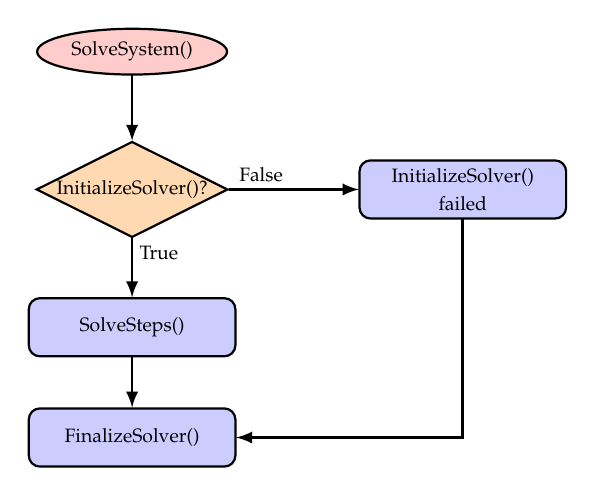
\begin{tikzpicture}[node distance = 2cm, auto, thick,scale=0.7, every node/.style={scale=0.7}]
			% Place nodes
			\node [cloud] (solveSystem) {SolveSystem()};
%			\node [wideblock, below of=init_solver_specific] (initializeSolver) {InitializeSolver()};
			\node [decision, below of=solveSystem] (decisionInitSolver) {InitializeSolver()?};
			\node [wideblock, right of=decisionInitSolver, node distance=6cm] (initFailed) {InitializeSolver() failed};
			\node [wideblock, below of=decisionInitSolver, node distance=2.5cm] (solveSteps) {SolveSteps()};
			\node [wideblock, below of=solveSteps] (finalizeSolver) {FinalizeSolver()};
			
			\path [arrow] (solveSystem) -- (decisionInitSolver);
			\path [arrow] (decisionInitSolver) -- node [near start] {False}(initFailed);
			\path [arrow] (decisionInitSolver) -- node [near start] {True}(solveSteps);
			\path [arrow] (solveSteps) -- (finalizeSolver);
			\path [arrow] (initFailed) |- (finalizeSolver);
	\end{tikzpicture}
  \caption{Basic solver flow chart for SolveSystem(). This flow chart is the same for static solver and for time integration.}
	\label{fig_solver_time_integration}
\end{figure}

%++++++++++++++++++++++++++++++++++++++++++++++++++++++++++++++++++++++++
\begin{figure}[tbp]
  \centering
	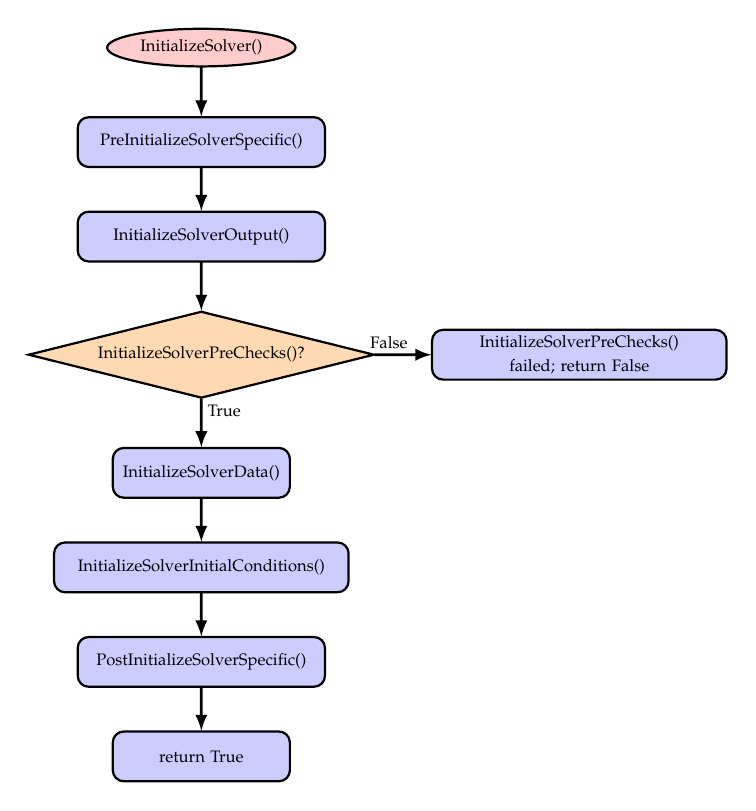
\begin{tikzpicture}[node distance = 2cm, auto, thick,scale=0.6, every node/.style={scale=0.6}]
			% Place nodes
			\node [cloud] (initializeSolver) {InitializeSolver()};
			\node [wideblock, text width=5cm, below of=initializeSolver] (preInitializeSolverSpecific) {PreInitializeSolverSpecific()};
			\node [wideblock, text width=5cm, below of=preInitializeSolverSpecific] (initializeSolverOutput) {InitializeSolverOutput()};
			\node [decision, aspect=4, text width=6cm, below of=initializeSolverOutput] (initializeSolverPreChecks) {InitializeSolverPreChecks()?};
			
			\node [wideblock, text width=6cm, right of=initializeSolverPreChecks, node distance=8cm] (initFailed) {InitializeSolverPreChecks() failed; return False};
			\node [wideblock, below of=initializeSolverPreChecks, node distance=2.5cm] (initializeSolverData) {InitializeSolverData()};
			\node [wideblock, text width=6cm, below of=initializeSolverData] (initializeSolverInitialConditions) {InitializeSolverInitialConditions()};
			\node [wideblock, text width=5cm, below of=initializeSolverInitialConditions] (postInitializeSolverSpecific) {PostInitializeSolverSpecific()};
			\node [wideblock, below of=postInitializeSolverSpecific] (finished) {return True};
			
			\path [arrow] (initializeSolver) -- (preInitializeSolverSpecific);
			\path [arrow] (preInitializeSolverSpecific) -- (initializeSolverOutput);
			\path [arrow] (initializeSolverOutput) -- (initializeSolverPreChecks);
			\path [arrow] (initializeSolverPreChecks) -- node [near start] {False}(initFailed);
			\path [arrow] (initializeSolverPreChecks) -- node [near start] {True}(initializeSolverData);
			\path [arrow] (initializeSolverData) -- (initializeSolverInitialConditions);
			\path [arrow] (initializeSolverInitialConditions) -- (postInitializeSolverSpecific);
			\path [arrow] (postInitializeSolverSpecific) -- (finished);
	\end{tikzpicture}
  \caption{Basic solver flow chart for function InitializeSolver().}
	\label{fig_solver_initialize_solver}
\end{figure}

%++++++++++++++++++++++++++++++++++++++++++++++++++++++++++++++++++++++++
\begin{figure}[tbp]
  \centering
	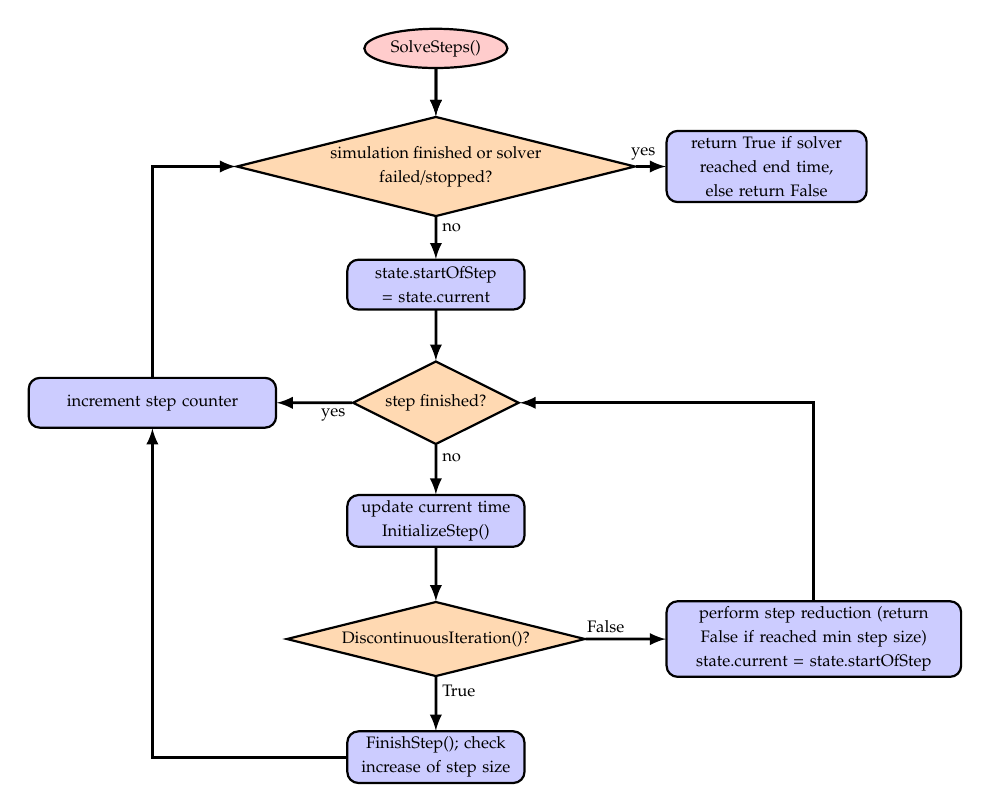
\begin{tikzpicture}[node distance = 2cm, auto, thick,scale=0.6, every node/.style={scale=0.6}]
			% Place nodes
			\node [cloud] (solveSteps) {SolveSteps()};
			\node [decision, aspect=4, text width=5cm, below of=solveSteps] (solveStepsLoop) {simulation finished or solver failed/stopped?};
			
			\node [wideblock, text width=4cm, right of=solveStepsLoop, node distance=7cm] (solveStepsLoopFinished) {return True if solver reached end time, else return False};
			\node [wideblock, below of=solveStepsLoop, node distance=2.5cm] (setStartOfStepState) {state.startOfStep = state.current};
			\node [decision, below of=setStartOfStepState] (stepReduction) {step finished?};
			\node [wideblock, text width=5cm, left of=stepReduction, node distance=6cm] (finishStep) {increment step counter};
			\node [wideblock, below of=stepReduction, yshift = -0.5cm] (initializeStep) {update current time\\InitializeStep()};
			\node [decision, aspect=4, text width=5cm, below of=initializeStep] (discontinuousIteration) {DiscontinuousIteration()?};
			\node [wideblock, text width=6cm, right of=discontinuousIteration, node distance=8cm] (discontinuousIterationFailed) {perform step reduction (return False if reached min step size)\\state.current = state.startOfStep};
			\node [wideblock, below of=discontinuousIteration, node distance=2.5cm] (finishDiscIt) {FinishStep(); check increase of step size};
			
			\path [arrow] (solveSteps) -- (solveStepsLoop);
			\path [arrow] (solveStepsLoop) -- node [near start] {no}(setStartOfStepState);
			\path [arrow] (solveStepsLoop) -- node [near start] {yes}(solveStepsLoopFinished);
			\path [arrow] (setStartOfStepState) -- (stepReduction);
			\path [arrow] (stepReduction) -- node [near start] {no}(initializeStep);
			\path [arrow] (stepReduction) -- node [near start] {yes}(finishStep);
			\path [arrow] (finishStep) |- (solveStepsLoop);
			
			\path [arrow] (initializeStep) -- (discontinuousIteration);
			\path [arrow] (discontinuousIteration) -- node [near start] {False}(discontinuousIterationFailed);
			\path [arrow] (discontinuousIteration) -- node [near start] {True}(finishDiscIt);
			\path [arrow] (solveSteps) -- (solveStepsLoop);
			\path [arrow] (discontinuousIterationFailed) |- (stepReduction);
			\path [arrow] (finishDiscIt) -| (finishStep);
	\end{tikzpicture}
  \caption{Solver flow chart for SolveSteps(), which is the inner loop of the solver.}
	\label{fig_solver_solve_steps}
\end{figure}

%++++++++++++++++++++++++++++++++++++++++++++++++++++++++++++++++++++++++
\begin{figure}[tbp]
  \centering
	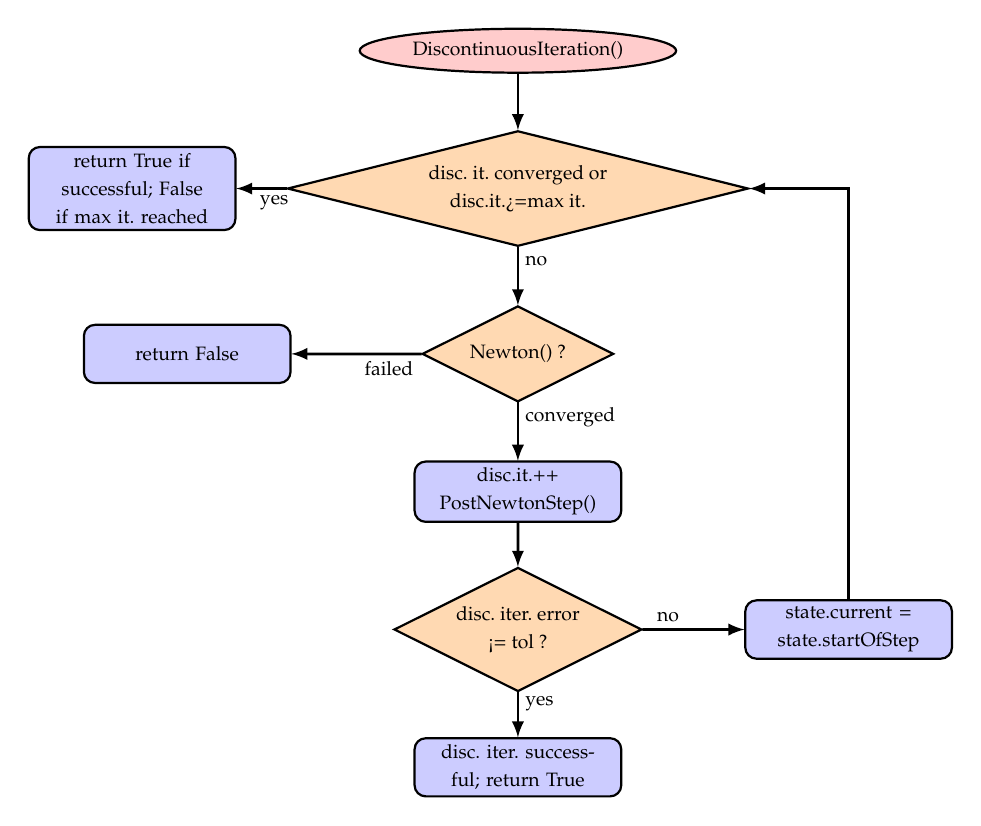
\begin{tikzpicture}[node distance = 2cm, auto, thick,scale=0.7, every node/.style={scale=0.7}]
			% Place nodes
			\node [cloud] (discontinuousIteration) {DiscontinuousIteration()};
			\node [decision, aspect=4, text width=5cm, below of=discontinuousIteration] (discontinuousIterationLoop) {disc.\ it.\ converged or disc.it.>=max it.};
			\node [wideblock, left of=discontinuousIterationLoop, node distance=6cm, xshift=-1cm] (discItTerminate) {return True if successful; False if max it.\ reached};
			
			%\node [wideblock, text width=4cm, right of=discontinuousIterationLoop, node distance=7cm] (discontinuousIterationLoopFinished) {return True if converged, else return False};
			
			\node [decision, below of=discontinuousIterationLoop, yshift = -0.5cm] (newtonLoop) {Newton() ?};
			\node [wideblock, left of=newtonLoop, node distance=6cm] (newtonFailed) {return False};
			\node [wideblock, below of=newtonLoop, yshift = -0.5cm] (postNewtonStep) {disc.it.++\\PostNewtonStep()};

			\node [decision, below of=postNewtonStep] (postNewtonStepError) {disc.\ iter.\ error\\ <= tol ?};
			\node [wideblock, right of=postNewtonStepError, node distance=6cm] (resetDiscIt) {state.current = state.startOfStep};
			\node [wideblock, below of=postNewtonStepError, yshift = -0.5cm] (discItSuccessful) {disc.\ iter.\ successful; return True};
			
			%compute Residual
			%check Residual
			%compute jacobian
			%steepest decent
			%check convergence
			%... end of Newton: set state back to start of step (except for data variables)
			
			\path [arrow] (discontinuousIteration) -- (discontinuousIterationLoop);
			\path [arrow] (discontinuousIterationLoop) -- node [near start] {no}(newtonLoop);
			\path [arrow] (discontinuousIterationLoop) -- node [near start] {yes}(discItTerminate);
			
			%\path [arrow] (discontinuousIterationLoop) -- (newtonLoop);
			\path [arrow] (newtonLoop) -- node [near start] {failed}(newtonFailed);
			\path [arrow] (newtonLoop) -- node [near start] {converged}(postNewtonStep);

			\path [arrow] (postNewtonStep) -- (postNewtonStepError);
			\path [arrow] (postNewtonStepError) -- node [near start] {no}(resetDiscIt);
			\path [arrow] (postNewtonStepError) -- node [near start] {yes}(discItSuccessful);

			\path [arrow] (resetDiscIt) |- (discontinuousIterationLoop);
			%\path [arrow] (finishStep) |- (solveStepsLoop);
			%
			%\path [arrow] (initializeStep) -- (discontinuousIteration);
			%\path [arrow] (discontinuousIteration) -- node [near start] {False}(discontinuousIterationFailed);
			%\path [arrow] (discontinuousIteration) -- node [near start] {True}(finishDiscIt);
			%\path [arrow] (solveSteps) -- (solveStepsLoop);
			%\path [arrow] (discontinuousIterationFailed) |- (stepReduction);
	\end{tikzpicture}
  \caption{Solver flow chart for DiscontinuousIteration(), which is run for every solved step inside the static/dynamic solvers. If the DiscontinuousIteration() returns False, 
	SolveSteps() will try to reduce the step size.}
	\label{fig_solver_discontinuous_iteration}
\end{figure}

%++++++++++++++++++++++++++++++++++++++++++++++++++++++++++++++++++++++++
\begin{figure}[tbp]
  \centering
	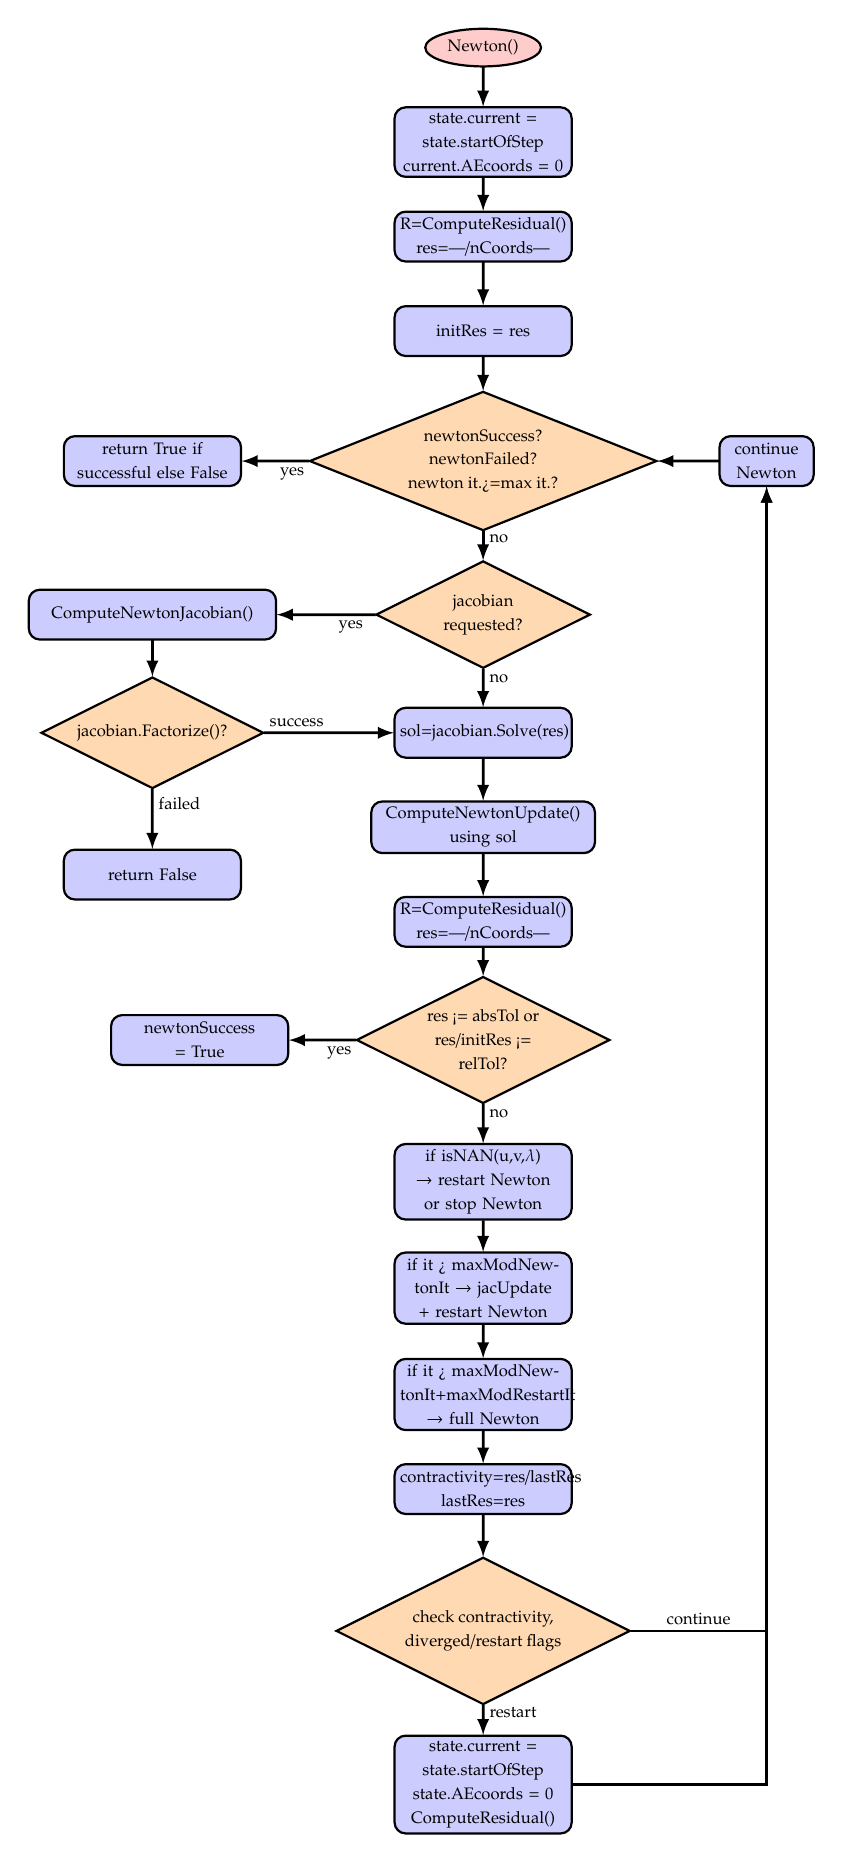
\begin{tikzpicture}[node distance = 2cm, auto, thick,scale=0.6, every node/.style={scale=0.6}]
			% Place nodes
			\node [cloud] (newtonIteration) {Newton()};
			\node [wideblock, below of=newtonIteration] (initNewton) {state.current = state.startOfStep\\ current.AEcoords = 0};
			\node [wideblock, below of=initNewton] (residual) {R=ComputeResidual()\\res=|/nCoords|};
			\node [wideblock, below of=residual] (initResidual) {initRes = res};

			\node [decision, aspect=2.5, text width=4cm, below of=initResidual, yshift = -0.25cm] (newtonLoop) {newtonSuccess?\\newtonFailed?\\newton it.>=max it.?};
			\node [wideblock, left of=newtonLoop, node distance=6cm, xshift=-1cm] (newtonTerminate) {return True if successful else False};
			\node [block, right of=newtonLoop, node distance=6cm] (continueNewton) {continue Newton};
			\node [decision, below of=newtonLoop, yshift = -0.75cm] (jacUpdate) {jacobian requested?};

			\node [wideblock, text width = 5cm, left of=jacUpdate, node distance=7cm] (updateJacobian) {ComputeNewtonJacobian()};
			\node [decision, text width = 4cm, below of=updateJacobian, yshift = -0.0cm] (factorizeJacobian) {jacobian.Factorize()?};
			\node [wideblock, below of=factorizeJacobian, yshift = -1.0cm] (jacFactorizeFailed) {return False};

			\node [wideblock, below of=jacUpdate, yshift = -0.5cm] (jacobianSolve) {sol=jacobian.Solve(res)};
			\node [wideblock, below of=jacobianSolve, text width=4.5cm, yshift = -0.0cm] (newtonUpdate) {ComputeNewtonUpdate() using sol};
			\node [wideblock, below of=newtonUpdate] (residual2) {R=ComputeResidual()\\res=|/nCoords|};

			%\node [wideblock, below of=residual2] (adaptInitResidual) {initResidual = max(res,initRes)};
			\node [decision, below of=residual2] (evalTolerances) {res <= absTol or res/initRes <= relTol?};
			\node [wideblock, left of=evalTolerances, node distance=6cm] (newtonConverged) {newtonSuccess = True};
			\node [wideblock, below of=evalTolerances, yshift=-1cm] (checkDivergence) {if isNAN(u,v,$\lambda$)\\ $\ra$ restart Newton or stop Newton};
			\node [wideblock, below of=checkDivergence, yshift=-0.25cm] (checkIterations) {if it > maxModNewtonIt $\ra$ jacUpdate + restart Newton};
			\node [wideblock, below of=checkIterations, yshift=-0.25cm] (checkIterations2) {if it > maxModNewtonIt+maxModRestartIt $\ra$ full Newton};
			\node [wideblock, below of=checkIterations2, yshift=-0.cm] (checkContractivity) {contractivity=res/lastRes\\lastRes=res};
			\node [decision, text width=4.5cm, below of=checkContractivity, yshift=-0.5cm] (restartNewton) {check contractivity, diverged/restart flags};
			
			\node [wideblock, below of=restartNewton, yshift=-1.25cm] (restartNewtonIteration) {state.current = state.startOfStep\\ state.AEcoords = 0\\ComputeResidual()};

			%adapt initial residual
			%!converged: 
			%  - check divergence
			%  if modNewton:
			%    - check max mod newton its reached? yes: compute Jac
			%    - check contractivity ==> compute Jac / switch to full newton


			%\node [decision, below of=postNewtonStep] (postNewtonStepError) {disc.\ iter.\ error\\ <= tol ?};
			%\node [wideblock, right of=postNewtonStepError, node distance=6cm] (resetDiscIt) {state.current = state.startOfStep};
			%\node [wideblock, below of=postNewtonStepError, yshift = -0.5cm] (discItSuccessful) {disc.\ iter.\ successful; return True};
			
	
			\path [arrow] (newtonIteration) -- (initNewton);
			\path [arrow] (initNewton) -- (residual);
			\path [arrow] (residual) -- (initResidual);

			\path [arrow] (initResidual) -- (newtonLoop);
			\path [arrow] (newtonLoop) -- node [near start] {no}(jacUpdate);
			\path [arrow] (newtonLoop) -- node [near start] {yes}(newtonTerminate);
			%
			\path [arrow] (jacUpdate) -- node [near start] {no}(jacobianSolve);
			\path [arrow] (jacUpdate) -- node [near start] {yes}(updateJacobian);

			\path [arrow] (updateJacobian) -- (factorizeJacobian);
			\path [arrow] (factorizeJacobian) -- node [near start] {failed}(jacFactorizeFailed);
			\path [arrow] (factorizeJacobian) -- node [near start] {success}(jacobianSolve);
%
			\path [arrow] (jacobianSolve) -- (newtonUpdate);
			\path [arrow] (newtonUpdate) -- (residual2);

			\path [arrow] (residual2) -- (evalTolerances);
			\path [arrow] (evalTolerances) -- node [near start] {yes}(newtonConverged);
			\path [arrow] (evalTolerances) -- node [near start] {no}(checkDivergence);
			\path [arrow] (checkDivergence) -- (checkIterations);
			\path [arrow] (checkIterations) -- (checkIterations2);
			\path [arrow] (checkIterations2) -- (checkContractivity);
			\path [arrow] (checkContractivity) -- (restartNewton);
			\path [arrow] (restartNewton) -- node [near start] {restart}(restartNewtonIteration);
			\path [arrow] (restartNewton) -| node [near start] {continue}(continueNewton);
			\path [arrow] (restartNewtonIteration) -| (continueNewton);
			
			\path [arrow] (continueNewton) -- (newtonLoop);

	\end{tikzpicture}
  \caption{Solver flow chart for Newton(), which is run inside the DiscontinuousIteration(). The shown case is valid for newtonResidualMode = 0.}
	\label{fig_solver_newton_iteration}
\end{figure}
\clearpage
%
\mysubsection{Explicit solvers}
\label{sec:ExplicitSolver}
Explicit solvers are in general only applicable for systems without constraints (i.e., no joints!). However, some solvers accept simple \texttt{CoordinateConstraint}, e.g., fixing coordinates to the ground.
Nevertheless, for constraint-free systems, e.g., with penalty constraints, can be solved for very high order and with great efficiency.
A list of explicit solvers is available, see \refSection{sec:DynamicSolverType}, for an overview of all implicit and explicit solvers.

The solution vector $\txi$ (denoted as $y$ in the literature \cite{Hairer1987}), which is defined as
\be
  \txi = [\qv\tp \;\; \dot \qv\tp \;\; \yv\tp ]\tp
\ee
and which includes \hac{ODE2} coordinates and velocities and \hac{ODE1} coordinates. All coordinates are computed without reference values.

The \hac{ODE1} and \hac{ODE2} equations of \eq{eq_systemEOM}, with $\tlambda=0$, are written in explicit form and converted to first order equations,
\bea \label{eq_systemEOM}
  \dot \qv &=& \vel \nonumber \\
  \ddot \vel & = &\Mm^{-1} \fv_\SO(\qv, \vel, t) \nonumber \\
  \dot \yv & = &\fv_\FO(\yv, t) \\
\eea
The system first order differential equations for explicit solvers thus read
\be
  \dot \txi = \fv_e (\txi, t)
\ee
%
\mysubsubsection{Explicit Runge-Kutta method}
\label{sec:rungekuttamethod}
Explicit time integration methods seek the solution $\txi_{t+h}$ at time $t+h$ for given initial value $\txi_{t}$ (at the beginning of one step $t$ or at the beginning of the simulation, $t=0$),
\be
  \txi_{t+h} = \txi_{t} + \Delta \txi\eqDot
\ee
For any given Runge-Kutta method, the integration of one step with step size $h$ is performed by an approximation
\be \label{s_stage_quadrature}
  \Delta \txi = \int _{t}^{t+h}\fv_e(\tau ,\txi(\tau ))d\tau \approx h\left[b_{1} \fv_e(t,\txi(t))+b_{2} \fv_e(t+c_{2} h,\txi(t+c_{2} h))+ \ldots +b_{s} \fv_e(t+\txi_{s} h,u(t+\txi_{s} h))\right] %  \eqref{GrindEQ__12_12_}
\ee
%
in which $t + c_{i}h$ is the time for stage $i$ and $b_i$ the according weight given in the integration formula.
Stages are within one step (therefor called one-step-methods), where $c_i=0$ represents the beginning of the step and $c_i=1$ the end.
Note that $c_{1}= 0$ for explicit integration formulas.

The unknown solution vectors $\txi$ at the stages are abbreviated by
\be
  \gv_{i} \approx \txi(t+c_{i} h) 
\ee
and computed by explicit integration (quadrature) formulas of lower order ($g_i$ not to be mixed up with algebraic equations!),
\be \label{eq_expl_RK_stages}
  \begin{array}{l} 
	{\gv_{1} =\txi_t} \\
	{\gv_{2} =\txi_t+ha_{21} \fv_e(t,\gv_{1} )} \\
	{\gv_{3} =\txi_t+h\left[a_{31} \fv_e(t,\gv_{1} )+a_{32} \fv_e(t+c_{2} h,\gv_{2} )\right]} \\
	{{\rm \; \; \; \; \; \; }\vdots } \\
	{\gv_{s} =\txi_t+h\left[a_{s1} \fv_e(t,\gv_{1} )+a_{s2} \fv_e(t+c_{2} h,\gv_{2} )+ \ldots +a_{s,s-1} \fv_e(t+c_{s-1} h,\gv_{s-1} )\right]} \end{array} 
\ee
After all vectors $\gv_i$ have been consecutively evaluated, the step is updated by \eq{s_stage_quadrature}.

Conventional explicit Runge-Kutta solvers, such as \texttt{ExplicitMidPoint}, \texttt{RK44} or \texttt{RK67} are based on 
fixed step size and users must control the error by choosing an appropriate global step size. The tableaus for some lower order methods
%\texttt{ExplicitEuler}, \texttt{ExplicitMidpoint} and \texttt{RK44} 
are given in Table \ref{tab:rungeKuttaTableaus}, using the structure
\begin{center}
\begin{tabular}{p{0.25cm}|p{0.25cm}} 
$\cv$ & $\Am$ \\ \hline 
~ & $\bv\tp$ \\ 
\end{tabular}
\end{center}
with
\begin{center}
\begin{tabular}{p{0.35cm}|p{0.35cm} p{0.35cm} p{0.35cm} p{0.35cm} } %\hline 
0 & 0 & & &\\ %\hline
$c_2$ & $a_{21}$ & $\ddots$ & & \\ %\hline
$\vdots$ & $\vdots$ & $\ddots$ & $\ddots$ & \\ %\hline
$c_s$ & $a_{s1}$ & $\cdots$ & $a_{s,s-1}$ & 0 \\ \hline
      & $b_{1}$ & $\cdots$ & $b_{s-1}$ & $b_{s}$ \\ %\hline
\end{tabular} 
\end{center}
%\be
  %\mp{\cv}{\Am}{}{\bv}, \quad \Am = \vr{a_{11}}{\cdots}{a_{1s}} {\vdots}{\cdots}{\vdots} {a_{s1}}{\cdots}{a_{ss}}
%\ee
with $\cv = [c_0=0, \; c_1, \; \ldots, \; c_s]$, $\bv = [b_0, \; b_1, \; \ldots, \; b_s]$, and $\Am$ having only entries in the 
lower left triangle.
For number of stages $s > 4$, the maximum order of explicit methods is lower than the number of stages, such as for \texttt{RK67}, which as order 6 but 7 stages.
%
\begin{table}
%
Explicit Euler method, number of stages $s=1$, order $p=1$:\\
\begin{center}
\begin{tabular}{p{0.1in}|p{0.1in}} %\hline 
0 & ~ \\ \hline 
~ & 1 \\ %\hline 
\end{tabular} \vspace{0.5cm}
\end{center}

Explicit midpoint rule, number of stages $s=2$, order $p=2$:\\
\begin{center}
\begin{tabular}{c|c c} %\hline 
0 &  &  \\ %\hline 
1/2 & 1/2 &  \\ \hline 
 & 0 & 1 \\ %\hline 
\end{tabular} \vspace{0.5cm}
\end{center}

Classical explicit Runge-Kutta method (RK44) , number of stages $s=4$, order $p=4$:\\
%\begin{tabular}{|p{0.2in}|p{0.2in}|p{0.2in}|p{0.2in}|p{0.2in}|} \hline 
\begin{center}
\begin{tabular}{c|c c c c }
0 &  &  &  &  \\ %\hline 
1/2 & 1/2 &  &  &  \\ %\hline 
1/2 & 0 & 1/2 &  &  \\ %\hline 
1 & 0 & 0 & 1 &  \\ \hline 
 & 1/6 & 1/3 & 1/3 & 1/6 \\ %\hline 
\end{tabular}
\end{center}
%
\caption{Several examples of tableaus for the implemented Runge-Kutta methods.}
\label{tab:rungeKuttaTableaus}
\end{table}
%
\mysubsubsection{Automatic step size control}
%
Advanced solvers, such as \texttt{ODE23} and \texttt{DOPRI5}, include automatic step size control\footnote{activated with
\texttt{timeIntegration.automaticStepSize = True} in simulationSettings}.

We estimate the error of a time step with current step size $h$ by
using an embedded Runge-Kutta formula, which includes two approximations \ref{s_stage_quadrature} of order $p$ and $\hat p = p-1$, which is obtained by using two different integration formulas with common coefficients $c_i$, but two sets of weights $b_i$ and $\hat b_i$, leading to two approximations $\txi$ and $\hat \txi$. These so-called embedded Runge-Kutta formulas are widely used, for details see Hairer et al.\ \cite{Hairer1987}. 

The according apporximations $\txi$ and $\hat \txi$ are used to estimate an error 
\be
  e_j=|\xi_j- \hat \xi_j|
\ee
for every component $j$ of the solution vector $\txi$.
A scaling is used for every component of the solution vector, evaluating at the beginning ($0$) and end ($1$) of the time step:
\be
  s_j = a_{tol} + r_{tol} \cdot \mathrm{max}(|\xi_{0j}|, |\xi_{1j}|) 
\ee
Then the relative, scaled, scalar error for the step, which needs to fulfill $err \le 1$, is computed as 
\be
  err = \sqrt{\frac 1 n \sum_{j=1}^n \left( \frac{\xi_{1j} - \hat \xi_{1j}}{s_j} \right)^2}
\ee
The optimal step size then reads
\be
  h_{opt} = h \cdot \left(\frac{1}{err} \right)^{(1/(q+1))}
\ee
Currently we use the suggested step size as
\be
  h_{new} = \mathrm{min}\left(h_{max}, \mathrm{min}\left(h \cdot f_{maxInc},  \mathrm{max}(h_{min}, f_{sfty} \cdot h_{opt}) \right) \right)
\ee
With the maximum step size $h_{max} = \frac{t_{start} - t_{end}}{n_{steps}}$ and the minimum step size $h_{min}$, given in the \texttt{timeIntegration} 
\texttt{simulationSettings}.
The factor $f_{maxInc}$ limits the increase of the current step size $h$, the factor $f_{sfty}$ is a safety factor for limiting the chosen step size relative to the optimal one in order to avoid frequent step rejections. 
If $h_{new} \le h$, the current step is accepted, otherwise the step is recomputed with $h_{new}$.
For more details, see Hairer et al.\ \cite{Hairer1987}.

\mysubsubsection{Stability limit}
Note that there are hard limitations for every explicit integration method regarding the step size. Especially for stiff systems (basically with high stiffness parameters and small masses, but also with restrictions to damping), the {\bf step size $h$ has an upper limit}: $h < h_{lim}$. Above that limit the method is inherently unstable, which needs to be considered both for constant and automatic step size selection.

\mysubsubsection{Explicit Lie group integrators}
All explicit solvers including the automatic step size solvers (DOPRI5, ODE23) have been equiped with Lie group integration functionality -- details will be published soon and some tests are made, but handle this with care.

Basically, the integration formulas, see \refSection{sec:rungekuttamethod} are extended for special rotation parameters.
Lie group integration is currently only available for \texttt{NodeRigidBodyRotVecLG} used in \texttt{ObjectRigidBody} (3D rigid body). 
\texttt{FFRFreducedOrder} will be extended to such nodes in the near future.
To get Lie group integrators running with rigid body models, all 3D node types need to be set to \texttt{NodeRigidBodyRotVecLG} and 
set \texttt{explicitIntegration.useLieGroupIntegration == True}.

\mysubsubsection{Constraints with explicit solvers}
Explicit solvers generally do not solve for algebraic constraints, except for very simple \texttt{CoordinateConstraint}. 
All connectors having the additional \texttt{type=Constraint}, see the according object in \refSection{sec:item:ObjectConnectorSpringDamper}ff., 
are in general not solvable by explicit solvers. 
Currently, only \texttt{CoordinateConstraint} with one coordinate fixed to ground can be accounted for, 
if \texttt{explicitIntegration.eliminateConstraints == True}. 
However, this offers the great flexibility to compute finite elements (imported meshes or ANCF beams) to be (partially) fixed to ground.
A \texttt{CoordinateConstraint} that fixes a coordinate with index $j$ to ground leads to the simple algebraic \hac{ODE2} equation
\be
	g_j(\qv) = 0 \quad \Leftrightarrow \quad  q_j = 0
\ee
which can be solved by the implemented explicit solvers by just setting $q_j = 0$ previously to every computation and $\dot q_j = 0$ after every \hac{RHS} evaluation.

NOTE that, if \texttt{explicitIntegration.eliminateConstraints == False}, constraints are ignored by the explicit solver (and all algebraic variables are set to zero). This may be wanted (e.g.\ to investigate the free motion of bodies), but in general leads to wrong and meaningless solution.

\mysubsection{Implicit (trapezoidal rule-based, Newmark, generalized-$\alpha$) solver}
\label{sec:ImplicitTrapezoidalSolver}
This solver represents a class of solvers, which are -- in the undamped case -- based on the implicit trapezoidal rule (in the view of Runge-Kutta methods). The interpolation of the quantities for one step includes the start and the end value of the time step, thus being called trapezoidal integration rule. In some special cases in Newmark's method \cite{Newmark1959}, the interpolation might only depend on the start value or the end value.

For now, all implemented solvers can be viewed as a generalization of Newmark's method, but there are called differently in the solver interfaces
\bi
  \item {\bf Implicit trapezoidal rule} ($=$ Newmark with $\beta = \frac 1 4$ and $\gamma = \frac 1 2$) 
	\item {\bf Newmark's method} \cite{Newmark1959}
	\item {\bf Generalized-$\alpha$ method} ($=$ generalized Newmark method with additional parameters), see Chung and Hulbert \cite{Chung1993} for the original method and Arnold and Br\"uls \cite{Arnold2007} for the application to multibody system dynamics.
\ei

\mysubsubsection{Newmark and generalized-$\alpha$ method}
Newmark's method has two parameters $\beta$ and $\gamma$. 
The main ideas are 
\bi
	\item Interpolate the displacements and the velocities linearly using the accelerations $\ddot \qv$ of the beginning of the time step (subindex '0') and the end of the time step (subindex 'T'). The \SON\ displacements and velocities and for \FON\ coordinates are given by (definition of $\aalg$ will become clear later):
\bea \label{eq_Newmark_interpolation}
		   \qv_T & = &      \qv_0 + h \dot \qv_0 + h^2 (\frac 1 2 -\beta) \aalg_0 + h^2 \beta \aalg_T \nonumber\\	
	\dot \qv_T & = & \dot \qv_0 + h (1-\gamma) \aalg_0 + h\gamma \aalg_T \nonumber\\
			  \yv_T & = & \yv_0 + h (1-\gamma_\FO) \vel^0_\FO + h\gamma_\FO \vel^T_\FO
\eea
	\item Solve the system equations at the end of the time step ($T$) for the unknown accelerations as well as for \FON\ and \AEN\ coordinates.
\ei
Remarks:
\bi
  \item The system of equations may be solved for accelerations $\ddot \qv$, but also for displacements $\qv$ or even velocities as unknowns while the remaining quantities are reconstructed from \eq{eq_Newmark_interpolation}. In case of displacements as unknowns, a scaling of the Jacobian is necessary, see later.
	\item For consistency reasons, one may set $\gamma_\FO = \gamma$, but {\bf currently we use} $\gamma_T = \frac 1 2$, leading to no numerical damping for \hac{ODE1} variables $\yv$.
	\item In the extension to the so-called generalized-$\alpha$ method \cite{Chung1993}, algorithmic accelerations $\aalg$ are used in \eq{eq_Newmark_interpolation}. Algorithmic accelerations are no longer equivalent to the time derivatives of displacements, $\aalg \neq \ddot \qv$; thus, both sets of variables are used independently. In case of Newmark or the implicit trapezoidal rule just use $\aalg = \ddot \qv$.
	\item For generalized-$\alpha$, the algorithmic accelerations $\aalg$ are computed from the recurrence relation
	\be
	   (1-\alpha_m)\av_T + \alpha_m \av_0 = (1-\alpha_f) \ddot \uv_T + \alpha_f \ddot \uv_0
	\ee
	which can be resolved for the unknown $\av_T$,
	\be
	  \av_T = \frac{(1-\alpha_f) \ddot \uv_T + \alpha_f \ddot \uv_0 - \alpha_m \av_0}{(1-\alpha_m)}
	\ee
	For the first step, one can simply use $\aalg_0 = \ddot \qv_0$.
\ei
%
\mysubsubsection{Parameter selection for generalized-$\alpha$}
\label{sec:parametersGeneralizedAlpha}
Compared to alternative implicit integration methods (including the Newmark method), the generalized-$\alpha$ integrator's parameters break down to one single parameter $\rho_\infty$, which allows to chose numerical damping in a practical way.

Based on a simple single DOF mass-spring-damper model \cite{Bauchau2011}, having the eigen frequency $\omega = 2\pi f$ with frequency $f$ and period $T=1/f$, the spectral radius $\rho$ for the integrator defines the amount of damping for a given step size $h$ related to $T$, thus using the dimensionless step size $\bar h=h/T$.

In \fig{fig:spectralRadius} the spectral radius is shown versus $\bar h$ for various spectral radii at infinity $\rho_\infty$. 
Here, $\rho_\infty$ specifies the numerical damping of very time step for large step sizes (or very high frequencies). An amount of $\rho_\infty=0.9$ means that high frequency parts of the system (($\bar h \gg 1$); high compared to the step rate) are damped to $90\%$ in every step, reducing an initial value $1$ to $2.66e-5$ after 100 steps, which is already much larger than usual physical damping in many cases.

Furthermore, low frequency parts of the system ($\bar h \ll 1$) receive almost no numerical damping, see again \fig{fig:spectralRadius}. 
Exemplarily, consider $\rho$ a low frequency situation with different $\rho_\infty$:
\bi
  \item $\rho(\bar h=0.01, \rho_\infty=0.9) = 1 - 1.13\cdot 10^{-9}$
	\item $\rho(\bar h=0.01, \rho_\infty=0.6) = 1 - 1.22\cdot 10^{-7}$
\ei
which shows that numerical damping is very low for moderately small step sizes (100 steps for one oscillation).

Obviously, $\rho_\infty$ does not have a large influence for very high or low frequencies in the system as long as it is $\neq 1$ and we could even use $\rho_\infty=0$.
Regarding differential algebraic equations (DAEs), $\rho_\infty<1$ allows to integrate index 3 DAEs. Typically a value of $\rho_\infty=0.7$ leads to a stable integration, but values depend on the structure of the multibody system.

Once having chosen $\rho_\infty$, all other parameters follow automatically \cite{Chung1993}, regarding the $\alpha$s
\be
	\alpha_m = \frac{2 \rho_\infty - 1}{\rho_\infty + 1}, \quad
	\alpha_f = \frac{\rho_\infty}{\rho_\infty + 1}
\ee
and Newmarks's parameters,
\be
	\gamma = \frac{1}{2} - \alpha_m + \alpha_f, \quad 
	\beta = \frac{1}{4}(1- \alpha_m + \alpha_f)^2
\ee

\begin{figure}%
\begin{center}
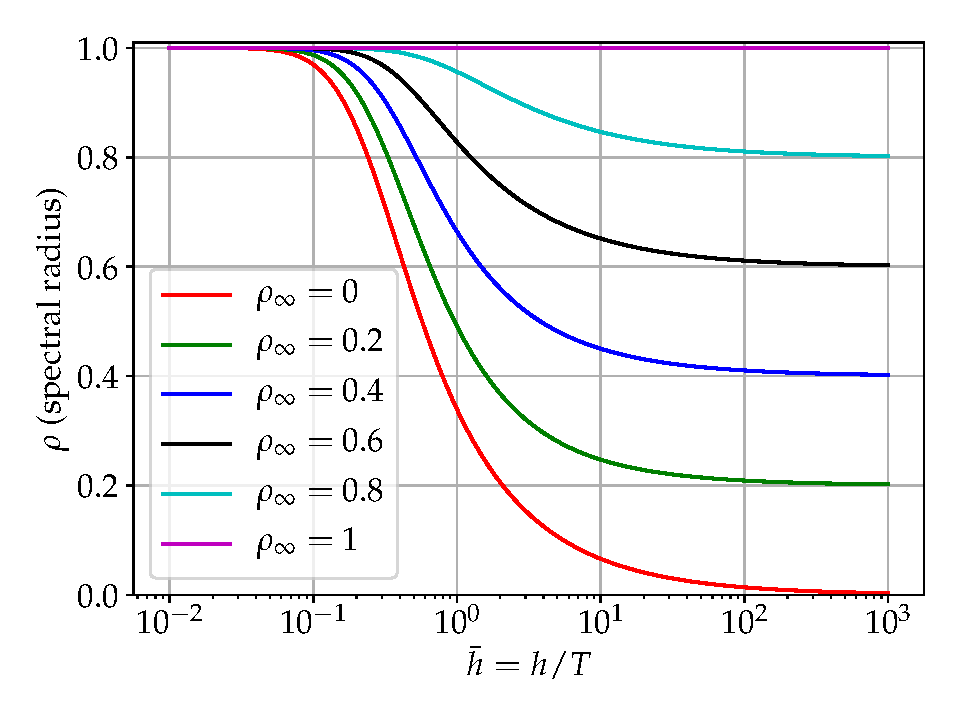
\includegraphics[width=0.6\columnwidth]{figures/spectralRadiusZeta0}%
\end{center}
\caption{Spectral radius for generalized-$\alpha$ method depending on dimensionless step size $\bar h=h/T$, in which
$T$ is the period of an equivalent single DOF mass-spring-damper system.}%
\label{fig:spectralRadius}%
\end{figure}


% ++++++++++++++++++++++++++++++++++++++++++++++++++++++++
% ++++++++++++++++++++++++++++++++++++++++++++++++++++++++
\mysubsubsection{Newton iteration}
\newcommand{\avu}{\ddot \qv} %unknown acceleration
%
\newcommand{\GA}{{G\alpha}} %abbreviation to mark equations, residuals, etc.
%
Thus, the residuals at the end of the time step ($T$) read (put all terms to \hac{LHS}):
\bea \label{eq_generalizedAlphaRes}
  \rv^\GA_\SO &=& \Mm \ddot \qv_T + \frac{\partial \gv}{\partial \qv^\mathrm{T}} \tlambda_T - \fv_\SO(\qv_T, \dot \qv_T, t) = 0\\
  \rv^\GA_\FO &=& \dot \yv_T + \frac{\partial \gv}{\partial \yv^\mathrm{T}} \tlambda_T - \fv_\FO(\yv_T, t) = 0\\
	\rv^\GA_\AE &=& \gv(\qv_T, \dot \qv_T, \yv_T, \tlambda_T, t) = 0
\eea
%
We consider two options for \SON: (A) solve for unknown accelerations $\avu_T$,  or (B) for unknown displacements $\qv_T$.

\mysubsubsubsection{(A) Solve for unknown accelerations}
%
The unknowns for the Newton method then are
\be \label{eq_Newton_unknowns1}
  \txi^\GA_{k+1} = \vr{\avu_T}{\yv_T}{\tlambda_T}
\ee
and at the beginning of the step, we have
\be \label{eq_Newton_unknowns2}
  \txi^\GA_{k} = \vr{\avu_0}{\yv_0}{\tlambda_0}
\ee
For the Newton method, we need to compute an update for the unknowns of \eq{eq_Newton_unknowns1}, using the previous residual $\rv_{k}$ and the inverse of the Jacobian $\Jm_{k}$ of Newton iteration $k$,
\be
  \txi^\GA_{k+1} = \txi^\GA_{k} - \Jm^{-1} \left( \txi^\GA_{k} \right) \cdot \rv^\GA \left( \txi^\GA_{k} \right)
\ee

% +++++++++++++++++++++
% Jacobians for Newmark
The Jacobian has the following $3 \times 3$ structure,
\be
  \Jm = \mr{\Jm_{\SO\SO}}{\Jm_{\SO\FO}}{\Jm_{\SO\AE}}
           {\Jm_{\FO\SO}}{\Jm_{\FO\FO}}{\Jm_{\FO\AE}}
           {\Jm_{\AE\SO}}{\Jm_{\AE\FO}}{\Jm_{\AE\AE}}
			= \mr{\Jm_{\SO\SO}}{\Null}{\Jm_{\SO\AE}}
           {\Null}{\Jm_{\FO\FO}}{\Jm_{\FO\AE}}
           {\Jm_{\AE\SO}}{\Jm_{\AE\FO}}{\Jm_{\AE\AE}}
\ee
in which we consider $\Jm_{\FO\SO}$ and $\Jm_{\SO\FO}$ to vanish in the current implementations, which means that coupling of \hac{ODE1} and \hac{ODE2} coordinates is only possible due to algebraic equations.

The remaining terms in the Jacobian read
\bea
  \Jm_{\SO\SO}&=&\frac{\partial \rv^\GA_\SO}{\partial \avu} 
							 = \frac{\partial \rv^\GA_\SO}{\partial \qv} \frac{\partial \qv}{\partial \avu} 
							   + \frac{\partial \rv^\GA_\SO}{\partial \dot \qv} \frac{\partial \dot \qv}{\partial \avu} 
							 = h^2 \beta \Km + h \gamma \Dm
							 \nonumber \\
	\Jm_{\SO\AE}&=&\frac{\partial \rv^\GA_\SO}{\partial \tlambda} 
	             = \frac{\partial \gv}{\partial \qv} \quad (\mbox{or } \frac{\partial \gv}{\partial \dot \qv} \mbox{ for constraints at velocity level)} \nonumber \\
	\Jm_{\FO\FO}&=&\frac{\partial \rv^\GA_\FO}{\partial \yv} \nonumber \\
	\Jm_{\AE\SO}&=&\frac{\partial \rv^\GA_\AE}{\partial \avu}
	             = \frac{\partial \gv}{\partial \avu}
	             = \frac{\partial \gv}{\partial \qv} \frac{\partial \qv}{\partial \avu} + 
							   \frac{\partial \gv}{\partial \dot \qv} \frac{\partial \dot \qv}{\partial \avu}
							 = h^2 \beta \frac{\partial \gv}{\partial \qv} 
							   + h \gamma \frac{\partial \gv}{\partial \dot \qv}
							\nonumber \\
	\Jm_{\AE\FO}&=&\frac{\partial \rv^\GA_\AE}{\partial \yv} \nonumber \\
	\Jm_{\AE\AE}&=&\frac{\partial \rv^\GA_\AE}{\partial \tlambda}
							 = \frac{\partial \gv}{\partial \tlambda}
\eea
%
Once an update $\qv^\mathrm{Newton}_{k+1}$ has been computed, the interpolation formulas \eqref{eq_Newmark_interpolation} need to be evaluated before the next residual and Jacobian can be computed.
%
\mysubsubsubsection{(B) Solve for unknown displacements}
%
This approach is similar to the previous approach and follows exactly the algorithm given by Arnold and Br\"uls \cite{Arnold2007}, however, extended for \hac{ODE1} variables, which are integrated by the (undamped) trapezoidal rule.
Documentation will be added lateron.

\mysubsubsection{Initial accelerations}
%
For the solvers based on the implicit trapezoidal rule, initial accelerations are necessary in order to significantly increase the accuracy
of the first time step.
For this reason, the constraints $\gv(\qv_0, \dot \qv_0, \yv_0, \tlambda_0, t) = 0$ in \eq{eq_system_EOM} are differentiated w.r.t.\ time,
\be \label{eq_initialAccelerationsVel}
	\dot \gv(\qv_0, \dot \qv_0, \yv_0, \tlambda_0, t) = 
	\frac{\partial \gv}{\partial \qv} \dot \qv_0 + 
	\frac{\partial \gv}{\partial \dot \qv}\ddot \qv_0 +
	\frac{\partial \gv}{\partial \yv} \dot \yv_0 + 
	\frac{\partial \gv}{\partial \tlambda} \dot \tlambda +
	\frac{\partial \gv}{\partial t} = 0 \eqDot 
\ee
Currently, we assume $\frac{\partial \gv}{\partial \tlambda} = 0$ for all further derivations on initial accelerations.
For velocity level constraints, \eq{eq_initialAccelerationsVel} is used to extract initial accelerations $\ddot \qv_0$,
\be
  \frac{\partial \gv}{\partial \dot \qv}\ddot \qv_0 = %\Gm_{ia-vel} \ddot \qv_0 = \gv_{ia-vel}(\qv_0, \dot \qv_0, \yv_0, t) = 
	  -\frac{\partial \gv}{\partial \qv} \dot \qv_0 
		-\frac{\partial \gv}{\partial \yv} \dot \yv_0
	  %-\frac{\partial \gv}{\partial \tlambda} \dot \tlambda 
		-	\frac{\partial \gv}{\partial t} \eqDot
\ee
%
Finally, the equations for the computation of the initial accelerations read for velocity level constraints,
note that $\yv_{init}$ are the nodal initial values for $\yv$,
\be \label{eq_initialAccelerationsVel2}
  \mr{\Mm}{\Null}{\frac{\partial \gv}{\partial \dot \qv^\mathrm{T}}} 
	   {\Null}{\Im}{\Null}
		 {\frac{\partial \gv}{\partial \dot \qv}}{\Null}{\Null}
		 \vr{\ddot \qv_0}{\yv_0}{\tlambda_0}
   = \vr{\fv_\SO(\qv_T, \dot \qv_T, t)}{\yv_{init}}
	      {-\frac{\partial \gv}{\partial \qv} \dot \qv_0-\frac{\partial \gv}{\partial \yv} \dot \yv_0 - \frac{\partial \gv}{\partial t}}  \eqComma
\ee
%
The term $\frac{\partial \gv}{\partial t}$ can only occur in case of user functions and therefore currently not implemented, and the \hac{ODE1} term $\frac{\partial \gv}{\partial \yv} = 0$ is not used yet in constraints.

For position level constraints, we assume $\frac{\partial \gv}{\partial \dot \qv} = 0$ and $\frac{\partial \gv}{\partial \yv} = 0$ in \eq{eq_initialAccelerationsVel} and perform a second derivation w.r.t.\ time,
\be \label{eq_initialAccelerationsPos}
	\ddot \gv(\qv_0, \dot \qv_0, \yv_0, \tlambda_0, t) = 
	\frac{\partial^2 \gv}{\partial \qv^2} \dot \qv_0^2 + 
	2 \frac{\partial^2 \gv}{\partial \qv \partial t} \dot \qv_0 + 
	\frac{\partial \gv}{\partial \qv} \ddot \qv_0 + 
	%\frac{\partial^2 \gv}{\partial \yv^2} \dot \yv_0^2 + 
	%\frac{\partial \gv}{\partial \yv} \ddot \yv_0 + 
	\frac{\partial^2 \gv}{\partial t^2} = 0 \eqDot
\ee
For position level constraints, \eq{eq_initialAccelerationsPos} is used to extract initial accelerations $\ddot \qv_0$,
\be
  \frac{\partial \gv}{\partial \qv} \ddot \qv_0 = %\Gm_{ia-pos} \ddot \qv_0 = \gv_{ia-pos}(\qv_0, \dot \qv_0, \yv_0, t) = 
	- 2 \frac{\partial^2 \gv}{\partial \qv \partial t} \dot \qv_0
	- \frac{\partial^2 \gv}{\partial \qv^2} \dot \qv_0^2
	%- \frac{\partial^2 \gv}{\partial \yv^2} \dot \yv_0^2
	%- \frac{\partial \gv}{\partial \yv} \ddot \yv_0
	- \frac{\partial^2 \gv}{\partial t^2} \eqDot
\ee
Finally, the equations for the computation of the initial accelerations for position level constraints read
\be \label{eq_initialAccelerationsPos2}
  \mr{\Mm}{\Null}{\frac{\partial \gv}{\partial \qv^\mathrm{T}}} 
	   {\Null}{\Im}{\Null}
		 {\frac{\partial \gv}{\partial \qv} }{\Null}{\Null}
		 \vr{\ddot \qv_0}{\yv_0}{\tlambda_0}
   = \vr{\fv_\SO(\qv_T, \dot \qv_T, t)}{\yv_{init}}
	      {- 2 \frac{\partial^2 \gv}{\partial \qv \partial t} \dot \qv_0 - \frac{\partial^2 \gv}{\partial \qv^2} \dot \qv_0^2	- \frac{\partial^2 \gv}{\partial t^2}}  \eqComma
\ee
%in which $\gv_{ia}$ and $\Gm_{ia}$ are placeholder for either $\gv_{ia-pos}$ and $\Gm_{ia-pos}$ for position level constraints and $\gv_{ia-vel}$ resp.\ $\Gm_{ia-vel}$ for velocity level constraints.
The linear system of equations \ref{eq_initialAccelerationsVel2} or \ref{eq_initialAccelerationsPos2} is solved prior to an implicit time integration if 
\bi
  \item[] \texttt{simulationSettings.timeIntegration.generalizedAlpha.computeInitialAccelerations = True} 
\ei
which is the default value.
%
%The unknowns for the Newton method are
%\be \label{eq_Newton_unknowns}
  %\qv^\mathrm{Newton} = \vr{\avu^T_\SO}{\vel^T_\FO}{\qv^T_\AE}
%\ee
%For the Newton method, we need to compute an update for the unknowns \eq{eq_Newton_unknowns}, using the known residual $\rv_{i-1}$ and the inverse of the Jacobian $\Jm_{i-1}$ of step $i-1$,
%\be
  %\qv^\mathrm{Newton}_{i} = \qv^\mathrm{Newton}_{i-1} - \Jm^{-1}\left( \qv^\mathrm{Newton}_{i-1}\right) \rv\left( \qv^\mathrm{Newton}_{i-1}\right)
%%  \qv^\mathrm{Newton}_{i} = \qv^\mathrm{Newton}_{i-1} - \Jm^{-1}_{i-1} \Rm\left(\avu^T_{\SO,i-1},\,\vel^T_{\FO,i-1},\,\qv^T_{\AE,i-1} \right)
%\ee
%
%% +++++++++++++++++++++
%% Jacobians for Newmark
%The Jacobian has the following $3 \times 3$ structure,
%\be
  %\Jm = \mr{\Jm_{\SO\SO}}{\Jm_{\SO\FO}}{\Jm_{\SO\AE}}
           %{\Jm_{\FO\SO}}{\Jm_{\FO\FO}}{\Jm_{\FO\AE}}
           %{\Jm_{\AE\SO}}  {\Jm_{\AE\FO}}  {\Jm_{\AE\AE}}
%\ee
%Note that currently, all terms related to '$\FO$' are not implemented. The other terms are only evaluated in the specific jacobian computation, if according flags are set in GetAvailableJacobian(). 
%Otherwise, the constraint needs to be implemented as object which can employ all kinds of coordinates, which do not depend on coordinates of markers.
%
%The available Jacobians need to be rewritten in terms of the Newton unkowns \eqref{eq_Newton_unknowns}, and thus read
%\bea
  %\Jm_{\SO\SO}&=&\frac{\partial \fv^\mathrm{Newmark}_\SO}{\partial \avu_\SO^\mathrm{T}} 
							 %= \frac{\partial \fv^\mathrm{Newmark}_\SO}{\partial \qv_\SO^\mathrm{T}} \frac{\qv_\SO}{\avu_\SO^\mathrm{T}} 
							   %+ \frac{\partial \fv^\mathrm{Newmark}_\SO}{\partial \dot \qv_\SO^\mathrm{T}} \frac{\dot \qv_\SO}{\avu_\SO^\mathrm{T}} 
							 %= h^2 \beta \Km + h \gamma \Dm
							 %\nonumber \\
	%\Jm_{\SO\AE}&=&\frac{\partial \fv^\mathrm{Newmark}_\SO}{\partial \qv_\AE^\mathrm{T}} 
	             %= \frac{\partial \gv}{\partial \qv_\SO^\mathrm{T}} \nonumber \\
	%\Jm_{\AE\SO}&=&\frac{\partial \fv^\mathrm{Newmark}_\AE}{\partial \avu_\SO^\mathrm{T}} 
	             %= \frac{\partial \gv}{\partial \avu_\SO^\mathrm{T}}
	             %= \frac{\partial \gv}{\partial \qv_\SO^\mathrm{T}} \frac{\qv_\SO}{\avu_\SO^\mathrm{T}} + \frac{\partial \gv}{\partial \dot \qv_\SO^\mathrm{T}} \frac{\dot \qv_\SO}{\avu_\SO^\mathrm{T}}
							 %= h^2 \beta \frac{\partial \gv}{\partial \qv_\SO^\mathrm{T}} 
							   %+ h \gamma \frac{\partial \gv}{\partial \dot \qv_\SO^\mathrm{T}}
							%\nonumber \\
	%\Jm_{\AE\AE}&=&\frac{\partial \fv^\mathrm{Newmark}_\AE}{\partial \qv_\AE^\mathrm{T}}
							 %= \frac{\partial \gv}{\partial \qv_\AE^\mathrm{T}}
%\eea
%Note that the derivative $\frac{\qv_\SO}{\avu_\SO^\mathrm{T}}$ follows from the Newmark interpolation \eqref{eq_Newmark_interpolation} using the relation between $\qv^T_\SO$ and $\avu^T_\SO$. The tangent stiffness matrix $\Km$ must also include derivatives of applied forces $\fv^a$, which is currently not implemented.
%Furthermore, the Jacobian is not symmetric, which could be obtained by according scaling.

%
% +++++++++++++++++++++
% Newton update formula
%Once an update $\qv^\mathrm{Newton}_{k+1}$ has been computed, the interpolation formulas \eqref{eq_Newmark_interpolation} need to be evaluated before the next residual and Jacobian can be computed.

%\mysubsubsection{Jacobian computation}
%
%The computation of the global jacobian matrix is time consuming for the static solver or implicit time integration.
%The equations are split into \SON, \FON and \AEN parts. From this structure, in the general non-symmetric case, 3 $\times$ 3 submatrices result for the jacobian.
%Every submatrix of the jacobian has a certain meaning and needs to be computed individually.
%Specifically, in implicit time integration the \SON $\times$ \SON term includes the (tangent) stiffness matrix and the mass matrix.
%
%For efficient computation purpose, the elements provide a list of flags, which determine the dependencies as well as available (analytical) functions to compute the local (object) jacobian:
%\bi
  %\item ODE2\_ODE2 $\ldots$ derivative of \hac{ODE2} equations with respect to \hac{ODE2} variables
  %\item ODE2\_ODE2\_t $\ldots$ derivative of \hac{ODE2} equations with respect to ODE2\_t (velocity) variables
  %\item ODE1\_ODE1 $\ldots$ derivative of ODE1 equations with respect to ODE1 variables (NOT YET AVAILABLE)
  %\item AE\_ODE2 $\ldots$ derivative of AE (algebraic) equations with respect to \hac{ODE2} variables
  %\item AE\_ODE2\_t $\ldots$ derivative of AE (algebraic) equations with respect to ODE2\_t (velocity) variables (NOT YET AVAILABLE)
  %\item AE\_ODE1 $\ldots$ derivative of AE (algebraic) equations with respect to ODE1 variables (NOT YET AVAILABLE)
  %\item AE\_AE $\ldots$ derivative of AE (algebraic) equations with respect to AE variables
%\ei
%If one of these flags is set (binary; e.g.ODE2\_ODE2 + ODE2\_ODE2\_t), then the according local jacobian is computed and assembled into the global jacobian in the static or implicit dynamic solver.
%
%Jacobians can also be supplied in analytical (function) form, which is indicated by an additional flag with the same name but an additional term '\_function', e.g.\ 'ODE2\_ODE2\_function' indicates that the derivative of ODE2 equations with respect to its ODE2 coordinates is provided in an analytical form (this is the tangent stiffness matrix).
%
%Two {\bf object} functions are used to compute the local jacobians:
%\bi
  %\item \texttt{\bf ComputeJacobianODE2\_ODE2(Matrix\& jacobian, Matrix\& jacobian\_ODE2\_t)}: computes the \texttt{ODE2\_ODE2} and \texttt{ODE2\_ODE2\_t} jacobians
	%\item \texttt{\bf ComputeJacobianAE(Matrix\& jacobian, Matrix\& jacobian\_AE)}: computes the \texttt{AE\_ODE2} and \texttt{AE\_AE} jacobians of the object ITSELF
%\ei
%Two {\bf connector} functions are used to compute the local jacobians, using \texttt{MarkerData}:
%\bi
  %\item \texttt{\bf ComputeJacobianODE2\_ODE2(Matrix\& jacobian, Matrix\& jacobian\_ODE2\_t, const MarkerDataStructure\& markerData)}: computes the \texttt{ODE2\_ODE2} and \texttt{ODE2\_ODE2\_t} jacobians of the connector; e.g.\ for spring-damper
	%\item \texttt{\bf ComputeJacobianAE(Matrix\& jacobian, Matrix\& jacobian\_AE, const MarkerDataStructure\& markerData)}: computes the \texttt{AE\_ODE2} and \texttt{AE\_AE} jacobians of the connector; e.g.\ for coordinate constraint
%\ei
%
%The system jacobian has the structure (\SO = ODE2, \FO = ODE1, $\AE$ = AE; $\bar \fv_\SO$ = according system residual including dynamic (mass matrix) terms in time integration; $\gv_\AE$ = algebraic equations):
%\be
  %\bigmr
  %{\frac{\partial \bar \fv_\SO}{\partial \qv_\SO}} {0} {\left(\frac{\partial \gv_\AE}{\partial \qv_\SO}\right)^T}
  %{0} {\frac{\partial \fv_\FO}{\partial \qv_\FO}} {\left(\frac{\partial \gv_\AE}{\partial \qv_\FO}\right)^T}
	%{\frac{\partial \gv_\AE}{\partial \qv_\SO}} {\frac{\partial \gv_\AE}{\partial \qv_\FO}} {\frac{\partial \gv_\AE}{\partial \qv_\AE}}
%\ee
%
%Two system jacobian functions are currently available:
%\bi
  %\item \texttt{\bf JacobianODE2RHS(temp, newton, factorODE2, factorODE2\_t, jacobian\_ODE2, jacobian\_ODE2\_t)}: compute analytical/numerical differentiation of ODE2RHS w.r.t. ODE2 and ODE2\_t coordinates; if analytical/functional version of jacobian is available and Newton flag 'useNumericalDifferentiation'=false, then the according jacobian is computed by its according function; results are 2 jacobians; the factors 'factor\_ODE2' and 'factor\_ODE2\_t' are used to scale the two jacobians; if a factor is zero, the according jacobian is not computed.
	%\item \texttt{\bf JacobianAE(temp, newton, jacobian, factorODE2, velocityLevel, fillIntoSystemMatrix)}: 
		%compute constraint jacobian of AE with respect to ODE2 ('fillIntoSystemMatrix'=true: also w.r.t. [ODE1] and AE) coordinates $\ra$ direct computation given by access functions; 'factorODE2' is used to scale the ODE2-part of the jacobian (to avoid postmultiplication); velocityLevel = true: velocityLevel constraints are used, if available; 'fillIntoSystemMatrix'=true: fill in both $\frac{\partial \bar \fv_\AE}{\partial \qv_\SO}$, $\frac{\partial \bar \fv_\AE}{\partial \qv_\SO}^T$ AND $\frac{\partial \bar \fv_\AE}{\partial \qv_\AE}$ at according locations into system matrix; 'fillIntoSystemMatrix'=false: (this is a temporary/WORKAROUND function):
%\ei
%The system jacobian functions compute the local jacobians either by means of a provided function or numerically, using the 'NumericalDifferentiation' settings of 'Newton'.
%




%++++++++++++++++++++++++++++++++++++++++++++++++++++++++++++++++++++++++++
%++++++++++++++++++++++++++++++++++++++++++++++++++++++++++++++++++++++++++
%++++++++++++++++++++++++++++++++++++++++++++++++++++++++++++++++++++++++++
\newpage
\mysubsection{Optimization and parameter variation}
%
The real benefit of powerful multi-body simulation emerges only if combined with modern but also simple analysis and evaluation methods.
Therefore, \codeName\ has been integrated into the Python language, which offers a virtually unlimited number of methods of post-processing, evaluation and optimization.
In this section, two methods that are directly integrated into \codeName\ are revisited.
%
\label{sec:parameterVariation}
\mysubsubsection{Parameter Variation}
Parameter variation is one of the simplest tools to evaluate the dependency of the solution of a problem on certain parameters. This usually requires the computation of an objective (goal, result) value for a single computation (e.g, some error norm, maximum vibration amplitude, maximum stress, maximum deflection, etc.) for every computation. Furthermore, it needs to be run for a set of parameters, e.g., using a \texttt{for} loop.
While this could be done manually in \codeName , it is recommended to use built-in functions, which simplify evaluation and postprocessing and directly enable parallelization.
The according function \texttt{ParameterVariation(...)}, see \refSection{sec:processing:ParameterVariation}, performs a set of multi-dimensional parameter variations using a dictionary that describes the variation of parameters. See also \texttt{parameterVariationExample.py} in the \texttt{Examples} folder for a simple example showing a 2D parameter variation. The function \texttt{ParameterVariation(...)} requires the \texttt{multiprocessing} Python module which enables simple multi-threaded parallelism and has been tested for up to 80 cores on the LEO4 supercomputer at the University of Innsbruck, achieving a speedup of 50 as compared to a serial computation.

\mysubsubsection{Genetic Optimization}
\label{sec:optimization}
%
In engineering, we often need to find a set of unknown, independent parameters $\xv \in \Rcal^n$, $\xv$ being denoted as design variables and $\Rcal^n$ as design space. Sometimes, the design space is further subjected to constraints $\gv(\xv)=0$ as well as inequalities $\hv(x) \le 0$, which are not considered here. For simple solutions for constrained optimization problems using penalty methods, see the introductory literature \cite{Kiusalaas2013}.

Optimization problems are written in general in the form
\be
  \min\limits_{\xv} f(\xv), \quad \xv \in \Rcal^n \eqComma
\ee
where $f(\xv)$ denotes the {\it objective function} (={\it fitness function}). If we would like to maximize a function $\bar f(\xv)$, simply set $f(\xv)=-\bar f(\xv)$.

In engineering, the optimization problem could seek model parameters, e.g., the geometric dimensions and inertia parameters of a slider crank mechanism, in order to achieve smallest possible forces at the supports.
Another example is the identification of unknown physical parameters, such as stiffness, damping of friction. This can be achieved by comparing measurement and simulation data (e.g., accelerations measured at relevant parts of a machine). Lets assume that $\epsilon(t)$ is an error computed in every time step of a computation, then we can set the objective (=fitness) function, e.g., as 
\be
  f(x) = \frac 1 T \sqrt{\int_{t=0}^T \epsilon(t)^2 dt}
\ee
as the integral over the error $\epsilon$ between measurement and simulation data.
In general, a parameter variation would be sufficient to compute sufficient computations for all combinations within the design space, however, a 3D design space with 100 variations into every direction (e.g., varying the unknown damping coefficient between 1 and 100, etc.) would already require 1000.000 computations, which in an ideal case of 1 second/computation leads to almost 2 weeks of computation time.

As an alternative stochastic methods can be use to compute only the objective function for a smaller set of randomly generated design variables, which usually show regions with better parameters (lower $f$) in scatter plots.

{\bf Genetic algorithms}\cite{Goldberg1989, Whitley1994} can significantly reduce the necessary amount of objective function evaluations in order to perform the optimization. Genetic identification algorithms have been already successfully applied to multibody system dynamics\cite{Eder2014}. 

The general structure of a (canonical) genetic algorithm is depicted in \fig{fig_geneticOptimization}.
%++++++++++++++++++++++++++++++++++++++++++++++++++++++++++++++++++++++++
\begin{figure}[hb]
  \centering
	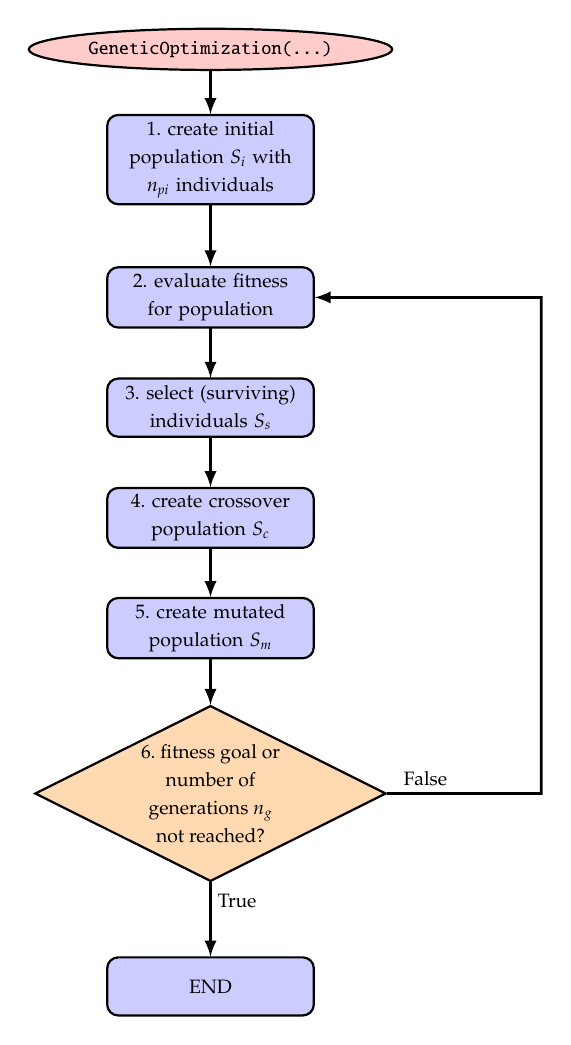
\begin{tikzpicture}[node distance = 2cm, auto, thick,scale=0.7, every node/.style={scale=0.7}]
			% Place nodes
			\node [cloud] (geneticOptimization) {\texttt{GeneticOptimization(...)}};
%			\node [wideblock, below of=init_solver_specific] (initializeSolver) {InitializeSolver()};
			\node [wideblock, below of=geneticOptimization, node distance=2cm] (initial) {1.\ create initial population $S_i$ with $n_{pi}$ individuals};
			\node [wideblock, below of=initial, node distance=2.5cm] (fitness) {2.\ evaluate fitness for population};
			\node [wideblock, below of=fitness] (surviving) {3.\ select (surviving) individuals $S_s$};
			\node [wideblock, below of=surviving] (crossover) {4.\ create crossover population $S_c$};
			\node [wideblock, below of=crossover] (mutation) {5.\ create mutated population $S_m$};
			\node [decision, below of=mutation, node distance=3cm] (decision) {6.\ fitness goal or number of generations $n_g$ not reached?};
			\node [wideblock, below of=decision, node distance=3.5cm] (end) {END};
			%
			\path [arrow] (geneticOptimization) -- (initial);
			\path [arrow] (initial) -- (fitness);
			\path [arrow] (fitness) -- (surviving);
			\path [arrow] (surviving) -- (crossover);
			\path [arrow] (crossover) -- (mutation);
			\path [arrow] (mutation) -- (decision);
			\path [arrow] (decision) -- node [near start] {False} +(6cm,0) |- (fitness);
			%(D.west) -- +(-1,0) |- node[pos=0.25] {No} (C);
			\path [arrow] (decision) -- node [near start] {True}(end);
	\end{tikzpicture}
  \caption{Basic solver flow chart genetic algorithm / optimization.}
	\label{fig_geneticOptimization}
\end{figure}
%
%\bn\setlength{\itemindent}{0.5cm}
  %\item START
  %\item create initial population $n_{pi}$
	%\item evaluate fitness for population\footnote{This is usually the time consuming part, which requires a single simulation run for every fitness evaluation}
	%\item select (surviving) individuals $S_s$
	%\item crossover $S_c$
	%\item mutation $S_m$
	%\item if fitness goal or number of generations $n_g$ not reached, continue with step
	%\item END
%\en
For details, see the cited literature. Here, we focus on the implementation of the function 
\texttt{GeneticOptimization(...)}, see \refSection{sec:processing:GeneticOptimization}.
The initial population (step 1) is created with \texttt{initialPopulationSize} individuals with uniformly distributed random design variables $[\xv_0, \ldots, \xv_{n_{pi}-1}]$\footnote{$\xv_i=[x_{i0}, x_{i1}, \ldots]$ being a set of genes, with single genes $x_{i0}$, $x_{i1}$, ... } in the search space, which is given in the dictionary \texttt{parameters}. Herafter (steps 2-6), we iteratively process a population for a certain \text{numberOfGenerations} generations.

In step 3, the surviving individuals $S_s$ with best fitness (smallest value from evaluation of \texttt{objectiveFunction}) are selected and considered further in the optimization. If the \texttt{distanceFactor} is used, the surviving individuals must be located within a certain distance (measured relative to the range of the search space) to all other surviving individuals. This option guarantees the search within several local minima, while a conventional search often converges to one single minimum.
Crossover (step 4)  is performed using a crossover of all available parameters of two randomly selected parents when generating children from the surviving individuals. The crossover of genes is performed only for a part of the new population, defined by \texttt{crossoverAmount}.

Finally, in step 5, we apply mutation to all genes, which extends the search to the surrounding design space of the individuals created by crossover. The mutation could be performed by means of certain distribution functions in order to focus on the currently best search regions. However, in the current implementation of \texttt{GeneticOptimization(...)} we simply use a uniform random variable to distribute the genes over a certain percentage of the design space, which is reduced in every generation defined by the \texttt{rangeReductionFactor} $r_r$. This allows us to restrict further search to a smaller subregion of the design space and in general allows a reduction of search space by means of $r_r^{n_g}$. In the ideal case, using sufficiently large population sizes and being lucky with the found random values, a range reduction factor $r_r=0.7$ reduces the search space by a factor of $100$ after every 13 generations, allowing to obtain 4 digits of accuracy for design variables after 26 generations for suitable optimization problems.

It should be noted that still this optimization method is based on random values and thus may fail occasionally for any problem case. In order to get reproducible results, set \texttt{randomizerInitialization} to any integer value (simply: 0) in order to get identical results for repeated runs. Setting the latter variable guarantees that the Python (numpy) randomizer creates the same series of random values for initial population, mutation, etc.








\clearpage

\mysection{References} 
coming soon!

\mysection{License} 

%\verbatiminput{././LICENSE.txt}
%\input{../../licenseEXUDYN.txt}
%\lstinputlisting{..\..\LICENSE.txt}
\plainlststyle
\lstinputlisting[breaklines=true, basicstyle=\ttm]{../../LICENSE.txt}
\end{document}


